%%%%%%%%%%%%%%%%%%%%%%%%%%%%%%%%%%%%%%%%%%%%%%%%%%%%%%%%%%%%%%%%%%%%%%%%
%
% Pangloss: Testing the reconstruction paper
%
%%%%%%%%%%%%%%%%%%%%%%%%%%%%%%%%%%%%%%%%%%%%%%%%%%%%%%%%%%%%%%%%%%%%%%%%

\documentclass[useAMS,usenatbib]{mn2e}
%% letterpaper
%% a4paper

% \voffset=-0.8in

% Packages:
\input psfig.sty
\usepackage{xspace}
\usepackage{graphicx}
\usepackage{amssymb}
\usepackage{amsmath}

% Macros:
% JOURNALS
\newcommand{\apj}{ApJ}
\newcommand{\apjl}{ApJL}
\newcommand{\apjs}{ApJS}
\newcommand{\mnras}{MNRAS}
\newcommand{\apss}{Ap \& SS}
\newcommand{\aap}{A\&A}
\newcommand{\aj}{AJ}
\newcommand{\prd}{Phys. Rev. D}
\newcommand{\nat}{Nature}
\newcommand{\araa}{ARA\&A}
\newcommand{\jgr}{J. Geophys. Res.}
\newcommand{\pasp}{PASP}

% MISC
\newcommand{\etal}{et~al.~}
\def\spose#1{\hbox  to 0pt{#1\hss}}  
\newcommand{\lta}{\mathrel{\spose{\lower 3pt\hbox{$\sim$}}\raise  2.0pt\hbox{$<$}}}
\newcommand{\gta}{\mathrel{\spose{\lower  3pt\hbox{$\sim$}}\raise 2.0pt\hbox{$>$}}}
\newcommand{\eg}{{\it e.g.\ }}
\newcommand{\ie}{{\it i.e.\ }}
\newcommand{\be}{\begin{equation}}
\newcommand{\ee}{\end{equation}}
\newcommand{\dee}{\, \mathrm{d} \!}
\newcommand{\bea}{\begin{eqnarray}}
\newcommand{\eea}{\end{eqnarray}}


% CROSS-REFERENCING
\def\Sref#1{Section~\ref{#1}\xspace}
\def\Fref#1{Figure~\ref{#1}\xspace}
\def\Tref#1{Table~\ref{#1}\xspace}
\def\Eref#1{Equation~\ref{#1}\xspace}
\def\Eqref#1{Eq.~(\ref{#1})\xspace}
\def\Aref#1{Appendix~\ref{#1}\xspace}

% UNITS
\newcommand{\kms}{\ifmmode  \,\rm km\,s^{-1} \else $\,\rm km\,s^{-1}  $ \fi }
\newcommand{\kpc}{\ifmmode  {\rm kpc}  \else ${\rm  kpc}$ \fi  }  
\newcommand{\pc}{\ifmmode  {\rm pc}  \else ${\rm pc}$ \fi  }  
\newcommand{\Msun}{\ifmmode {\rm M_{\odot}} \else ${\rm M_{\odot}}$ \fi} 
\newcommand{\Zsun}{\ifmmode {\rm Z_{\odot}} \else ${\rm Z_{\odot}}$ \fi} 
\newcommand{\yr}{\ifmmode yr^{-1} \else $yr^{-1}$ \fi} 
\newcommand{\hMsun}{\ifmmode h^{-1}\,\rm M_{\odot} \else $h^{-1}\,\rm M_{\odot}$ \fi}

% COSMOLOGY
\newcommand{\LCDM}{$\Lambda{\rm CDM}$}
\newcommand{\MS}{Millennium Simulation\xspace}

% LENSING
\def\zd{z_{\rm d}}
\def\zs{z_{\rm s}}
\def\Dd{D_{\rm d}}
\def\Ds{D_{\rm s}}

\def\Dt{D_{\Delta t}}

\def\Dds{D_{\rm ds}}
\def\Sigmacrit{\Sigma_{\rm crit}}
\def\REin{R_{\rm Ein}}
\def\MEin{M_{\rm Ein}}
\def\xkappa{\kappa_{\rm ext}}
\def\kappax{\kappa_{\rm ext}}
\def\kappaxtrue{\kappax^{\rm true}}
\def\kappah{\kappa_{\rm h}}
\def\kappav{\kappa_{\rm void}}
\def\kapparay{\kappa_{\rm raytrace}}
\def\kapparec{\kappa_{\rm reconstruction}}
\def\kappatrue{\kappa_{\rm true}}
\def\kappahalo{\kappa_{\rm halo}}
\def\Pkh{{\rm P}(\kappa_{\rm h})}
\def\Pk{{\rm P}(\kappa)}
\def\kappah{\kappa_{\rm h}}
\def\kappahk{\kappa_{{\rm h},k}}
\def\gammah{\gamma_{\rm h}}
\def\gammax{\gamma_{\rm ext}}


\def\sumkappah{\sum_{\rm halos} \kappa_{\rm halo}}
\def\sigt{\tilde{\sigma}}


% HALO MODEL PARAMETERS
\def\Mstar{M^{*}}
\def\logMstar{\log_{10}\left(\Mstar/\Msun\right)}
\def\Mstarobs{\Mstar_{\rm obs}}
\def\Mstarobsk{\Mstar_{{\rm obs},k}}
\def\Mhalo{M_{200}}
\def\Mh{M_{200}}
\def\logMhalo{\log_{10}\left(\Mhalo/\Msun\right)}
\def\Mhalok{M_{200,k}}
\def\Rhalo{R_{200}}
\def\chalo{c_{200}}

% SOFTWARE/HARDWARE
\def\SExtractor{{\sc SExtractor}\xspace}
\def\hst{{\it HST}\xspace}
\def\acs{\hst/ACS\xspace}
\def\galfit{{\sc galfit}\xspace}
\def\idl{{\sc idl}\xspace}
\def\python{{\sc python}\xspace}
\def\Pangloss{{\sc Pangloss}\xspace}

% TABLES:
\newcommand\nodata{ ~$\cdots$~ }%

% PROBABILITY THEORY
% % Phil:
% \def\pr{{\rm Pr}}
% \def\data{{\mathbf{d}}}
% \def\datap{{\mathbf{d}^{\rm p}}}
% \def\datai{d_i}
% \def\datapi{d^{\rm p}_i}
% Tom:
\def\pr{{\rm P}}
\def\data{{\mathcal{D}}}
\def\datap{{\data}^{\rm p}}
\def\datai{{\data}_i}
\def\datapi{{\data}^{\rm p}_i}

\def\sigi{\sigma_{\rm intrinsic}}

% COMMENTING
\usepackage[usenames]{color}
%\newcommand{\phil}[1]{\textcolor{blue}{\bf #1}}
%\newcommand{\matt}[1]{\textcolor{orange}{\bf #1}}
%\newcommand{\tom}[1]{\textcolor{OliveGreen}{\bf #1}}
\newcommand{\todo}[2]{\textcolor{red}{\bf TO DO (#1): #2}}
\newcommand{\flag}[1]{\textcolor{red}{\bf #1}}
\newcommand{\comment}[1]{}
\newcommand{\comments}[1]{}
\newcommand{\notes}[1]{\textcolor{cyan}{#1}}
\newcommand{\new}[1]{{\bf #1}}


\newcommand{\phil}[1]{#1}
\newcommand{\tom}[1]{#1}

% SPELLING:
\def\devided{divided\xspace}
\def\truely{truly\xspace}
\def\infered{inferred\xspace}
\def\correspends{corresponds\xspace}
\def\independant{independent\xspace}
\def\dependant{dependent\xspace}
\def\proceedure{procedure\xspace}
\def\propogate{propagate\xspace}
\def\propogates{propagates\xspace}
\def\succesful{successful\xspace}


\def\ioa{Institute of Astronomy, University of Cambridge,
  Madingley Rd, Cambridge, CB3 0HA, UK}
\def\oxford{Dept.\ of Physics, University of Oxford, 
  Keble Road, Oxford, OX1 3RH, UK}
\def\kipac{Kavli Institute for Particle Astrophysics and Cosmology, 
 Stanford University, 452 Lomita Mall, Stanford, CA 94035, USA}
\def\ucsb{Dept.\ of Physics, University of California, 
  Santa Barbara, CA 93106, USA}
\def\davis{Dept.\ of Physics, U.C.~Davis, Davis, CA 95616, USA}
\def\kapteyn{Kapteyn Astronomical Institute, University of Groningen, 
  P.O.Box 800, 9700 AV Groningen, The Netherlands}
\def\asiaa{Institute of Astronomy and Astrophysics, Academia Sinica, P.O.~Box 23-141, Taipei 10617, Taiwan}

\def\collettemail{\tt t.collett@ast.cam.ac.uk}

\def\packard{Packard Research Fellow}


%%%%%%%%%%%%%%%%%%%%%%%%%%%%%%%%%%%%%%%%%%%%%%%%%%%%%%%%%%%%%%%%%%%%%%%%%%%%%%

\title[Line of Sight Mass Reconstruction]
{Inferring Lensing Mass in the Universe \\
from Photometric Catalog Data}
    
\author[Collett \etal]{%
  Thomas~E.~Collett$^{1}$\thanks{\collettemail},
  Philip~J.~Marshall$^{2}$,
  Matthew~W.~Auger$^{1}$,
  Stefan~Hilbert$^{3}$,
\newauthor{%
  Sherry~H.~Suyu$^{4}$,
  Zachary~Greene$^{4}$,
  Tommaso~Treu$^{4}$\thanks{\packard},
  Christopher~D.~Fassnacht$^{5}$,}
\newauthor{%
  L\`eon~V.~E.~Koopmans$^{6}$,
  Roger~D.~Blandford$^{3}$} 
  \medskip\\
  $^1$\ioa\\
  $^2$\oxford\\
  $^3$\kipac\\
  $^4$\ucsb\\
  $^5$\davis\\
  $^6$\kapteyn
}

%%%%%%%%%%%%%%%%%%%%%%%%%%%%%%%%%%%%%%%%%%%%%%%%%%%%%%%%%%%%%%%%%%%%%%%%%%%%%%

\begin{document}
             
\date{to be submitted to MNRAS}
\pagerange{\pageref{firstpage}--\pageref{lastpage}}\pubyear{2012}

\maketitle           

\label{firstpage}

%%%%%%%%%%%%%%%%%%%%%%%%%%%%%%%%%%%%%%%%%%%%%%%%%%%%%%%%%%%%%%%%%%%%%%%%%%%%%%

\begin{abstract} 

Strong gravitational lenses can provide high precision cosmological distance
measurements; one of the most important sources of systematic error in these
estimates is the additional mass along the line of sight to the source. Weak
lensing by galaxies and groups in this beam can contribute an ``external
convergence'' $\xkappa$ that dominates the  uncertainty in the inferred
distances; likewise, it may also contaminate estimates of the luminosity of
objects at high redshift (such as reionisation-era proto-galaxies, and type Ia
supernovae standard candles).  We characterise this uncertainty by marginalising
over a probability density function for $\xkappa$: here, we investigate the use
of a simple halo model to estimate $\Pr(\xkappa)$ given noisy estimates of the
photometric redshift and stellar mass of galaxies observed in optical imaging
surveys of the field in question. We use mock catalogs from the Millenium
Simulation and compare our reconstructed $\Pr(\xkappa)$ to ray-traced $\kappa$ values,
we find that our model produces an unbiased estimator of $\kappax$,
For each lightcone the individual $\Pr(\xkappa)$ from this reconstruction process are
typically 1.8 times narrower than the global distribution of $\xkappa$ given perfect knowledge 
of the halo mass and redshift. After incorporating uncertainties on redshift and halo and stellar masses
we typically find that the reconstruction yields an improvement factor of 1.5. For each line of sight the
 $\Pr(\xkappa)$ can be formed before the investment of light-curve monitoring. By following up only the 
most costrained lines of sight a factor of 2 improvement over the global $\pr(\kappax)$ should be 
achievable.
\end{abstract}

% Full list of options at http://www.journals.uchicago.edu/ApJ/instruct.key.html

\begin{keywords}
  gravitational lensing   --
  methods: statistical    --
  galaxies: halos         --
  gaaxies: mass function  --
  cosmology: observations
\end{keywords}

\setcounter{footnote}{1}

%%%%%%%%%%%%%%%%%%%%%%%%%%%%%%%%%%%%%%%%%%%%%%%%%%%%%%%%%%%%%%%%%%%%%%%%%%%%%%

\section{Introduction}

Averaged over large areas of sky, the weak gravitational lensing effect can be
used to constrain the statistical properties of the matter density in the
Universe: every distant object we observe has had its shape distorted, and size
and total brightness magnified (or demagnified) by a compound lens constructed
from all the mass distributed between us and it.

This fact makes weak gravitational lensing a potentially important source of
systematic error for any estimate of luminosity or distance, an issue
raised for \eg 
type Ia supernovae by \citet[][]{Holz+Wald1998,Linder+Holz2004}, for
gamma ray bursts by \citet[][]{Oguri+Takahashi2006,Wang+Dai2011}, 
and for high redshift galaxies by \citet{BradacEtal2009}, among others. 
Along lines of sight containing strong gravitational lenses,
the effect has been found to be
particularly important, with foreground and background structures
having a significant effect on the inferred lensing cross-section
\citep[\eg][]{WongEtal2012} and distance ratios \citep[][]{DalalEtal2005}.
In time delay lens cosmography,
\citet{SuyuEtal2010} found that  the lensing effect of mass structures along the
(unusually over-dense)  line of sight to the quadruply-imaged radio source
B1608$+$656, the so-called ``external convergence,'' was the dominant source
of uncertainty in their 6\% measurement of Hubble's constant. 

How can we correct for this weak lensing error, and make
accurate measurements through the Universe? When inferring global quantities
(such as the cosmological parameters), averaging the results from a large
number of independent objects will tend to reduce the error, as the
ensemble-averaged convergence approaches zero for an unbiased sample
\citep[\eg][]{Linder+Holz2004}. If the sample is biased, however, some
residual systematic error will remain while the statistical uncertainty
decreases -- and this will be the case for any sample selected by the
brightness of the lensed object, or any other quantity that depends on
$\xkappa$. The latter class includes time delay lenses, which could be
either detected or selected 
based on their image separations, magnifications or quadruple image
configurations, all of which either increase or become more likely with
increasing $\kappa$. Large
samples of lenses are expected to be discovered in the next decade in
ground-based optical imaging surveys \citep{Oguri+Marshall2010} -- but these
samples will be image separation-limited, due to the surveys' relatively poor
($\sim 1$~arcsec) image quality. Some of the current sample of known time
delay lenses were detected in surveys like this: we might expect them to be
somewhat biased towards high values of $\xkappa$.

There are two broad approaches one could take at this point. First, one could
seek to characterise the lensed objects' selection function, and use this
understanding to derive a suitable correction to cosmological parameters
inferred assuming no $\xkappa$ at all. As pointed out by  \citet[][among
others]{Oguri+Takahashi2006}, to do this one would need  information about the
unlensed population of objects, and the population of lenses, and how the
objects were detected -- or to infer these hierarchically during the analysis.
Alternatively, one could simply accept all lenses provided, regardless of
their selection, and try to use any additional information that is available
to estimate the external convergence in each system on a case by case basis,
and hence optimize their joint analysis to produce a better-constrained result
\citep[as suggested by][]{Keeton+Zabludoff2004}. In this work we follow this
second approach, and use measurements of the positions, magnitude and colours
of galaxies close to lens lines of sight to try to infer the
external convergence at the lens position. 

Attempts to date at reconstructing the local and  line of sight mass
distribution in strong lens fields (what \citeauthor{WongEtal2011} call ``the
full environment'') have focused on photometric and  spectroscopic surveys to
detect galaxy groups and ascertain galaxies' membership,  and on understanding
the external shear apparently required by the strong lens models. Surveys by
\citet{Fassnacht+Lubin2002,AugerEtal2007,WilliamsEtal2006,MomchevaEtal2006}
all found groups of galaxies both hosting and lying  along the line of sight
to known gravitational lenses. Initial estimates of the effect of these
structures suggested the importance of assigning mass to both galaxy and group
halos, and to allowing for significant uncertainty in the centroids of group
halos. The probability density function (PDF) for the external convergence for
that lens, $\Pr(\xkappa)$, is the target for any reconstruction analysis, and
is the key quantity for any ensemble analysis, since by marginalising over it
we can correctly propagate the uncertainties due to weak lensing. Coming
closest to estimating this quantity from survey data, \citet{WongEtal2011} ran
Monte Carlo reconstructions of the mass in nine lens fields based on
\citeauthor{WilliamsEtal2006} and \citeauthor{MomchevaEtal2006}'s
photometric and spectroscopic measurements of galaxies close to the line of
sight, and compared the resulting predicted shear distributions with the
external shear demanded by the strong lens model. Their simulations show most
of the shear being generated by bright galaxies within 2~arcminutes of the
lens, and that both line of sight structures and the group of galaxies in each
lens plane contribute significant proportions of the shear. They find
significant discrepancies between the lens model shear and the Monte Carlo
predictions, and are unable to distinguish between the environment modelling
and the strong lens modelling as the cause of these discrepancies.

These observational investigations have provided very useful insight into the
problem.  Coming from a more theoretical direction, large numerical
simulations have been used to predict, from first principles, the distribution
of likely external shears and convergences along strong lens lines of sight. 
\citet{Holder+Schechter2003} and \citet{Dalal+Watson2004} carried out
ray-tracing calculations in N-body simulations to estimate the  distribution
of external shear values.  \citet{HilbertEtal2009} performed similar ray-tracing
experiments through the Millenium Simulation \citep{SpringelEtal2005},
generating a predicted $\xkappa$ at every position in a simulated sky. The
first step towards using this excellent calibration resource was taken by
\citet{SuyuEtal2010}, who selected Millenium Simulation lines of sight that a)
were found to contain a strong lens and b) had comparable apparent galaxy
overdensity in a 45 arcsec radius aperture down to $i < 24$. This overdensity
could be compared to the overdensity of the B1608$+$656 line of sight
\citep{FassnachtEtal2011}, and hence an estimate of  $\Pr(\xkappa)$ could be
made. 

In this paper, we bring these observational and theoretical approaches
together and  use numerical simulations to {\it test and calibrate} a
reconstruction of the  external convergence. Ray-tracing through the
simulations gives a ``truth'' that we can attempt to recover.  In this paper
we use the Millenium Simulation mock galaxy catalogs and ray-traced lensing
effects to test the accuracy of line of sight mass reconstructions.
Probabilistically ssigning mass and redshift to every observed galaxy in the
field around a time delay lens, we generate Monte Carlo sample line of sight
mass distributions, and estimate the external convergence due to each one.
This gives us a $\Pr(\xkappa)$ that can be propagated into further joint
inferences. We focus on time delay lens cosmography, and quantify our results
in terms of the uncertainty on the mean time delay distance to a test sample
of $N$ lenses (where for clarity each lens has the same deflector and source
redshift, and the same lens model and time delay uncertainty).

We aim to answer the following questions:
\begin{itemize}
\item Faint galaxies and other dark structures will not appear in a photometric
object catalog, but they will contribute convergence at some level. How much of
the total external convergence in a time delay lens system comes from visible
galaxies? How does this change as a function of magnitude cut? 
\item Can the true (ray-traced) convergence be recovered by halo model
reconstruction? What scatter and residual bias are induced in the ensemble 
distance estimate? Which aspects of the model dominate these uncertainties? 
\item When faced with a newly-detected lens, surrounded by galaxies on the sky,
we have some choices to make when planning follow-up observations.
Which are the most important galaxies, with regard to the external convergence
produced? Can nearby groups and clusters be straightforwardly accounted for? If
lenses with such massive structures nearby are discarded, what impact does that
have on the distance accuracy?
\end{itemize}

This paper is organized as follows. In~\Sref{sec:theory} we review the relevant
gravitational lensing theory, before introducing our simple reconstruction 
model in \Sref{sec:model}.  We then test this model in two phases: first, in
\Sref{sec:knownMh+z}, with known redshift and halo mass for every galaxy in a
lens field, in order to quantify the irreducible uncertainty due to unseen mass,
and second, in \Sref{sec:obsMstar+z}, with realistic observational uncertainties
on the field galaxies' stellar masses and redshifts. \comments{We then propagate all these
uncertainties through to the time delay distance in a toy sample of 100 lenses,
in \Sref{sec:distances}.} We discuss our results in \Sref{sec:discuss} before
concluding in \Sref{sec:conclude}.

Throughout this paper magnitudes are given in the AB system and
we adopt the Millenium Simulation's ``concordance'' parameters for our reference cosmology, \ie
$h=0.73$, $\Omega_m=0.25$ and $\Omega_\Lambda=0.75$, where the symbols indicate
the Hubble Constant in units of 100 km s$^{-1}$ Mpc$^{-1}$ and the matter and
dark energy density of the Universe in units of the critical density
.%\citep[e.g.\ ][]{KomEtal09}.


%%%%%%%%%%%%%%%%%%%%%%%%%%%%%%%%%%%%%%%%%%%%%%%%%%%%%%%%%%%%%%%%%%%%%%%%%%%%%%

\section{Theoretical Background}
\label{sec:theory}

%Time delay distances, and the mass sheet degeneracy - how kappa is degenerate in
%strong lens models (and magnifications).


Convergence, or Ricci focusing, occurs when a gravitational lens focuses the rays in a raybundle.
This focussing can cause distant objects to appear brighter, and larger than they would if the lens
 were removed.
The convergence from an isolated mass sheet is the ratio of the projected surface mass density
($\Sigma(D_{\mathrm{od}}\bmath{\theta})$) devided by the critical surface mass density at the redshift of the mass sheet ($\Sigma_{\rm cr}$),
\be
\kappa(\bmath{\theta})= \frac {\Sigma(D_{\mathrm{od}}\bmath{\theta})}{\Sigma_{\rm cr}(z)}
\ee
where 
\be \label{eq:sigcrit} 
\Sigma_{\rm cr}(z) \equiv \frac{c^2 D_{\rm os}}{4 \pi G D_{\rm od} D_{\rm ds}}.
\ee
and the D's are the angular diameter distances between the objects refered to in the subscripts: o is the observer, d is the deflector and s is the source. If the surface mass density of the sheet exceeds $\Sigma_{\rm cr}$, multiple images of the source can
occur, otherwise only one image will be observed, although that image will still be perturbed
relative to the unlensed case.

Strong lensing occurs when a massive object and background source are almost perfectly
aligned along a line of sight. The light from the background source is deflected by the
lens galaxy; this deflection allows multiple images of the background source to form
at stationary points of the time delay function. For an isolated lens, the time delay
function can be calculated from
\be \label{eq:T} 
\Delta t(\bmath{\theta},\bmath{\beta}) = \frac {1}{c} \frac{D_{\rm od} D_{\rm os}}{D_{\rm ds}} (1+z_{\rm d})\, \phi(\bmath{\theta},\bmath{\beta}),
\ee
where $\bmath{\theta}$ is the observed source position, $\bmath{\beta}$ is the 
unlensed source position, $z_{\rm d}$ is the redshift of the lens, $\phi(\bmath{\theta},\bmath{\beta})$ is
the Fermat potential. The Fermat potential is given by
\be \label{eq:FP}
\phi(\bmath{\theta},\bmath{\beta})\equiv \left[\frac{(\bmath{\theta}-\bmath{\beta})^2}{2}-\psi(\bmath{\theta}) \right], 
\ee
where $\psi(\bmath{\theta})$ is the lens potential, derived from the projected dimensionless
surface mass density, $\kappa(\bmath{\theta})$, by 
\be \label{eq:psikappa}
\kappa(\bmath{\theta})=\frac{1}{2}\nabla^2\psi(\bmath{\theta}).
\ee

Strong lenses sit in our real Universe -- they are not truely isolated;
there is some mass along the line of sight coming from intervening structures.
These structures may be physically associated with the lens e.g. other members
of a group or cluster, or they may be the result of chance alignments at any redshift. 
Whilst it is rare for three galaxies to line up well enough for both of the background sources
to be strongly lensed \citep{GavazziEtal2008,CollettEtal2012a}, the shear scale of dark matter halos
makes a partial alignment -- with the additional structure acting as a weak lens -- 
a near certainty, indeed \citet{Vale+White2003} and \citet{HilbertEtal2007} find that there
are no empty lightcones in a realistic universe. These additional structures induce an external shear
which can be recovered in the mass-modelling of the lens, but they can also introduce a convergence that
is undetectable from the image positions, shapes and relative fluxes; {\it the
mass sheet-degeneracy} \citep{FalcoEtal1985}.

If the intrinsic source brightness changes, the observed brightness in each image does not change
simultaneously - there is a time delay, $\Delta t$, between the brightness change in
each image. Despite the invariance of the image positions and fluxes, under the addition
of an external convergence (and appropriate re-scaling of the lens potential) the relative Fermat potential between the images is {\it not}
invariant, and so the time delay changes. As such it is necessary to include $\kappax$
in the lens modelling, if cosmological parameters are to be estimated accurately and
precisely from observed time delays \citep{SuyuEtal2010}.

\comments{
If the mass sheet is not physically associated with the lens galaxy, it can lie at any redshift. The effects of such a mass-sheet can be projected back onto the lens plane in the form of an effective convergence. We define this effective convergence in two limits.
\begin{itemize}
\item No significant perturbations along the line of sight, and \\
\item A single dominant perturber, relative to which all other perturbations are small.
\end{itemize}
We will refer to these cases as the magnification case (subscript $\mu$ in formulae), and the strong lensing case (subscript SL in formulae), respectively. We will ignore the additional case, of a compound lens, with several significant perturbers. 

The magnification case has no primary lens plane, and is chiefly relevant for the magnifications of distant objects. In the absence of a primary lens plane, we are free to define the effective convergence on any point; the effective convergence is the same, independant of the plane choosen. It can be shown \citep[\eg][]{xxx} that if there are several mass sheets at redshifts $\{z_{p}\}$, with convergences $\{\kappa_p =\Sigma_{p}/\Sigma_{\mathrm{cr}}(z_p)\}$, the effective convergence is given by
\be \label{eq:kappasummu}
\kappa_{\mathrm{effective,\mu}}=\sum_{p}\kappa_p.
\ee

In the stong lensing case, the presence of a significant perturber alters the
geometry of the system, and provides a primary lens plane. It is the primary
lens plane upon which we need to know $\kappa_{\mathrm{effective}}$, since
this is where the mass-sheet degeneracy is defined. Following Equations 20--32
of \citet{keeton2003}\flag{keeton2003}, it can be shown that the relevant
effective convergence is given by 
\be \label{eq:kappasumSL}
\kappa_{\mathrm{effective,SL}}=
{  
(1-\beta_{12})(\kappa-\beta_{12}(\kappa^2-\gamma^2))
\over
(1-\beta_{12}\kappa)^2-(\beta_{12}\gamma)^2
}
\ee
where $\kappa$ and $\gamma$ are, respectively, the convergence and shear
caused by the perturber, in their own plane and $\beta_{12}$ is a geometrical
scaling factor defined by
\be\label{eq:beta}
\beta_{12}={
D_{12} D_{\mathrm{os}}
\over
D_{\mathrm{o}1} D_{1\mathrm{s}}
}
\ee
where the D's are again angular diameter distances: the 1 (2) in the subscript
refers to the lower (higher) redshift object of the lens and perturber. For
the case that the mass sheet is in the lens plane, $\beta_{12} = 0$ and
$\kappa_{\mathrm{eff}}=\kappa$; if the mass-sheet is in the plane of the
observer, or source, $\beta_{12} = 1$ and $\kappa_{\mathrm{eff}}=0$; for a
mass-sheet at any other redshift $0<\beta_{12}<1$. In the case of several mass
sheets the effective convergences sum. In the limit that both $\kappa$ and
$\gamma$ are small, Equation \ref{eq:kappasumSL} reduces to 
\be \label{eq:kappasumSLweak}
\kappa_{\mathrm{effective,SL}}=(1-\beta_{12})\kappa;
\ee
it is this $\kappa_{\mathrm{effective,SL}}$ that we use as $\kappax$ for the
strong lensing time delay analysis in \ref{sec:Dt}.
}



\tom{The all-important calibration of the reconstruction has to be done
against Stefan's ray-traced kappas though -- so it is these that we have to
predict PDFs for, first and foremost. THEN we have to consider the question of
which kappa to use to correct the time delay distances: Stefan's kappa (as in
B1608 or RXJ1131), or kappa-keeton.}

The time-delay distance is defined as
\be \label{eq:dt}
\Dt \equiv (1+\zd) D_{\rm d} D_{\rm s}/D_{\rm ds},
\ee
with which Equation \ref{eq:T} can be rephrased as
\be
\Delta t(\bmath{\theta},\bmath{\beta})  =  \frac{\Dt}{c} \, \phi(\bmath{\theta},\bmath{\beta})    ,
\ee 
Since the time delays are proportional to $1/ (1- \kappax)$, if there is any external convergence, that is not included in the lens
modeling, then the time delay distance -- inferred assuming $\kappax = 0$ -- will be
$(1-\kappax)$ less than the true value of $\Dt$.
\be 
\label{eq:MassSheet:H0bias}
\Dt^{\rm{true}}=(1-\kappax) \Dt^{{\kappax = 0}}.
\ee
We can overcome this degeneracy if we have additional knowledge of $\kappax$.

For mass-sheets that are physically associated with the lens galaxy, the mass sheet
 affects the stellar dynamics of the
lens galaxy, so dynamical observations can break the internal
mass-sheet degeneracy by providing an additional estimate of the lens galaxy's mass
\citep[e.g.,][]{xxx}. 

In this work our aim is to quantify the lensing effect of mass-sheets that are not physically associated with the lens galaxy -- mass-sheets
lying infront or behind the lens -- and the uncertainties induced by reconstructing
those mass-sheets using simple prescriptions applied to potential astronomical observables.
\comments{We also aim to quantify how uncertainties in the
estimations of $\kappax$ propogate into uncertainties on the cosmological parametres
which can be inferred from measurements of $\Dt$.}


%%%%%%%%%%%%%%%%%%%%%%%%%%%%%%%%%%%%%%%%%%%%%%%%%%%%%%%%%%%%%%%%%%%%%%%%%%%%%%

\section{Estimating external convergence: The halo model approximation}
\label{sec:model}

%Weak lensing by NFW halos. Accounting for mass along the line of sight.
%Approximations to full ray tracing:
%
%Halos. N-body sims provide mass framework. MS halo catalog. Truncated spherical
%NFW approx based on virial masses. Stellar mass. Halo map corresponding to
%ray-traced kappa map, for illustration. Small-scale structure 

For real lines of sight, we would like to estimate the external convergence as best we can given all
data available. Typically this data is in the form of a photometric galaxy
catalog, containing positions, brightnesses, colours, and possibly spectra for each galaxy in the
field of the lens, down to some magnitude
limit. Since we can not observe the surface mass density of each halo
directy, we need some way of estimating
the mass of each halo in the catalog, so that we can compute its
contribution to the total $\kappax$ along the line of sight. This mass assignment recipe will be uncertain, but
can be calibrated with cosmological simulations.

% A source with known unlensed brightness e.g. a strongly lensed type Ia
% Supernova \flag{cite some SNe papers} or a source of known unlensed size \flag{ideas?}
% would break the mass-sheet degeneracy and provide a value for $\kappax$, but
% \flag{no?} such systems are currently known.

\subsection{Ray-tracing through simulated Lines of Sight}
\label{subsec:raytracing}
Cosmological dark matter simulations can be used to generate mock lines of
sight and can be raytraced through to give each mock sightline a $\kappax$ value...
\todo{Stefan}{Write section on how the ray tracing was done}

\subsection{Generating mock lightcones from simulations}

\todo{Stefan}{Write section on how halos are extracted from the MS n-body particles}



Transforming the photometometric galaxy catalogue into a  catalogue of
halo masses, positions, and redshifts, will enable us to attempt a
reconstruction of the convergence induced by every halo near a line of sight.
This is the subject of \ref{subsec:halos}. We also need to account for
the mass in the Universe that is not associated with the galaxies we can see
-- this is the subject of \ref{subsec:voids}. 


% % % % % % % % % % % % % % % % % % % % % % % % % % % % % % % % % % % % % % % 

\subsection{Halos}
\label{subsec:halos}

Cosmological dark matter simulations have shown that dark matter
halos are well approximated by NFW profiles \citep{NFW}, with a density
profile given by
\be\label{eq:rhonfw}
\rho(r) = 
\frac{\rho_0}{\left(r/r_{s}\right)
\left(1+r/r_{s}\right)^{2}},
\ee
where $r_{s}$ is a characteristic radius of the cluster, representing where
the density slope transitions from $r^{-1}$ to $r^{-3}$. This radius is related
to the virial radius of the halo by $r_{s}~=~r_{200}/c$, where $r_{200}$ is the radius at 
which 
\be
\rho(r_{200}) = 200\rho_{{\mathrm{crit}}}(z), \text{ where } \rho_{\mathrm{crit}}(z) \equiv \frac{3H^{2}(z)}{8\pi G}
\ee
and $c$ is the concentration parameter, which can be estimated from the halo's mass,
using a mass--concentration relation. Typically more massive halos are less concentrated,
but there is some scatter; we use the relation of \citet{Neto2007} to estimate $c$
from the mass enclosed within $r_{200}$, which we denote as $M_{200}$. The best fit relation of \citet{Neto2007} is given by
\be
c_{200} = 4.67 (M_{200}/10^{14} h^{-1} \Msun)^{-0.11}.
\ee
$\rho_0$ is calculated from the critical density and concentration parameter:
\be
\rho_0 = \rho_{\mathrm{crit}}(z)\frac{200}{3}\frac{c^{3}}{\ln(1+c)-c/(1+c)}.
\ee

Unphysically, if one integrates the density profile of an NFW profile, the total mass is divergent.
Similarly, if the universe is homogeneously populated with NFW halos, the projected surface mass along any
line of sight will also be divergant\footnote{At large radius, $\Sigma_{\rm
nfw} \propto R^{-2}$, but the differential number of halos centred within an
annulus of width $\dee R$ is given by $\dee N_{\rm annulus} \propto R \dee R$,
so  $\Sigma_{\rm total} \propto \int_{0}^{\infty} R^{-1} \dee R$, which
diverges logarithmically}. Since infinite mass is unphysical, the profile must
be truncated at some point. \todo{Tom}{Add notes on previous truncation results}. Several truncation profiles have been suggested \citep[e.g][]{BMO}, but beyond several virial radii, the amount of matter associated with a halo is likely to be low; \citet{NandraEtal2012} showed that the Universe's expansion can place an upper limit on the radius of NFW halos -- for cluster scale halos, this happens at around 25 times the NFW scale radius. In \Sref{sec:knownMh+z} we investigate how different truncations affect the recovered total convergence for a line of sight, using the truncated NFW profile of \citet{BMO}
\be\label{eq:bmoprofile}
\rho(r) = 
\frac{\rho_{\rm NFW} (r)}{1+\left(r/r_{t}\right)^2},
\ee
which is the same as the NFW profile in the limit that the truncation radius, $r_t$ goes to infinity. The convergence and shear for the BMO profile are given in Appendix \ref{appendix:halos}.


% % % % % % % % % % % % % % % % % % % % % % % % % % % % % % % % % % % % % % % 

\subsection{Calibration: Recovering the global $\pr(\kappax)$ using a void correction}
\label{subsec:voids}

Whilst halos contribute a positive convergence to $\kappax$, voids contribute
a negative convergence. When a raybundle passes through a  region of space
that is less dense than $\rho_{\rm cr}(z)$ the rays are de-focused\footnote{In
principle, the convergence caused by halos, is also caused by the overdensity,
but we neglect this effect since halos are typically much more dense than the
intergalactic medium}. Whilst the  full raytraced solution takes into account
the effect of voids, our reconstruction cannot -- the halo catalogue does not
include voids. In principle the absence of a halo could be taken to infer a
void, but the under-density of such a void is hard to infer. Neglecting voids
would lead to a heavily biased estimate of $\kappax$. We account for the voids
statistically; we reconstruct
the $\kappax$ contribution of halos for an ensemble of calibration sightlines
and form the joint distribution P($\kapparay,\sumkappah$). The calibration
can then be accounted for by marginalizing over all lines of sight with a similar
 $\sumkappah$.  We will refer to this calibration proceedure as the "void correction",
although it also accounts for all of the physics that our simple spherical halo prescription
neglects in a statistical manner. For each line of sight we create a $\pr(\kappax)$ from
\be
\pr(\kappax)=\int_{-\infty}^{+\infty}\pr(\kapparay',\tilde\kappa'_{\rm halos})W(\tilde\kappa_{\rm halos}-\tilde\kappa'_{\rm halos})\dee \tilde\kappa'_{\rm halos}
\ee
where $\tilde{\kappa}_{\rm halos}$ is the median of the reconstructed $\sumkappah$ for each line of sight.
Primed qunatities refer to all of the calibration sightlines and unprimed refers to the specific line of sight.
$W(\tilde\kappa_{\rm halos}-\tilde\kappa'_{\rm halos})$ is a weight function given by
\be
\label{eq:weighting}
W(\tilde\kappa_{\rm halos}-\tilde\kappa'_{\rm halos})=\exp\left(-\frac{1}{2}\left(\frac{\left(\tilde\kappa_{\rm halos}-\tilde\kappa'_{\rm halos}\right)^2}{\sigma^2}\right)\right)
\ee
We take $\sigma$ as 0.002- this is an overestimate of the uncertainty on $\tilde\kappa_{\rm halos}$, but ensures that the full distibution of void corrections is sampled, despite the finite number of calibration sightlines.



\comments{
For each reconstruction of a line of sight we can then draw a $\kappav$ from $\pr(\kappav)$ to correct for the
unseen voids. We refer to this corrective shift as $\kappav$. The void correction introduces a source of
error, since the value of $\kappav$ comes from the ensemble of calibration lines of sight rather than the individual
line of sight which is being reconstructed; this is unavoidable without modeling the $\kappax$ 
contribution of voids along a line of sight. To avoid potential biases we calculate $\pr(\kappav)$
from randomly selected calibration sightlines. The total $\kappax$ along the line of sight
is given by 
\be \label{eq:totalkappaxunweighted}
\pr(\kappax) = \left(\sum_{\rm halos} \pr(\kappa_{\rm halo})\right)-\pr(\kappav).
\ee

Once the void correction has been applied,the reconstruction should produce a 
reasonable estimate of $\pr(\kappax)$ for any single line of sight. However, from
the ray tracing results we know the global $\kappax$ distribution ${\rm U}(\kappax)$. We can use the global
 ${\rm U}(\kappax)$ as a prior by noting that the normalized sum of $\pr(\kapparec)$ from multiple lines
of sight should equal ${\rm U}(\kappax)$, \ie
\be \label{eq:prior}
{\rm U}(\kappax) = \lim_{N \to \infty} \sum_{i}^{N} \pr(\kappax)_{i} / N
\ee
In order to make Equation \ref{eq:prior} hold, we use Equation \ref{eq:totalkappaxunweighted} to calculate $\pr(\kappax)^{\rm unweighted}$ for the calibration lines of sight and
re-weight the reconstructions by:
\be \label{eq:weighting}
W(\kappa)=\left(\sum_{i}^{N} \pr(\kappax)_{i}^{\rm unweighted} /N \right) / \left({\rm U}(\kappax)\right)
\ee
such that the final reconstruction is given by 
\be \label{eq:totalkappax}
\pr(\kappax) = \left(\left(\sum_{\rm halos} \pr(\kappa_{\rm halo})\right)-\pr(\kappav)\right)(W(\kappa)).
\ee

}




\comments{
Whilst halos contribute a positive convergence to $\kappax$, voids contribute
a negative convergence. When a raybundle passes through a  region of space
that is less dense than $\rho_{\rm cr}(z)$ the rays are de-focused\footnote{In
principle, the convergence caused by halos, is also caused by the overdensity,
but we neglect this effect since halos are typically much more dense than the
intergalactic medium}. Whilst the  full raytraced solution takes into account
the effect of voids, our reconstruction cannot -- the halo catalogue does not
include voids. In principle the absence of a halo could be taken to infer a
void, but the under-density of such a void is hard to infer.
\tom{ Instead, we reconstruct 10000 lines of sight to give $\pr(\kapparec|kapparay)$
and invert the PDF using Bayes' theorem to give $\pr(\kapparay|\kapparec)$. For each lightcone we
can then get $\pr(\kapparay)$ by marginalizing over the reconstruction PDF, $\pr(\kapparec)$.
This recipe also ensures that we correctly recover the ensemble $\kapparay$ distribution, even in the case
of no input data.



 Instead, we shift
our $\kappax$ values so that $\langle\kappax\rangle=0$. We refer to this
corrective term as $\kappav$. The void correction introduces a source of
error, since the inferred value of $\kappav$ will depend on the properties of
the sightlines reconstructed, but this error shrinks with the number of
sightlines reconstructed. To avoid potential biases we calculate $\kappav$
from randomly selected sightlines. The total $\kappax$ along the line of sight
is given by 
\be \label{eq:totalkappax}
\kappax = \left(\sum_{\rm halos} \kappa_{\rm halo}\right)-\kappav.
\ee
}}

%%%%%%%%%%%%%%%%%%%%%%%%%%%%%%%%%%%%%%%%%%%%%%%%%%%%%%%%%%%%%%%%%%%%%%%%%%%%%%%%

\section{Testing the halo model approximation with known halo mass and redshift}
\label{sec:knownMh+z} 

\subsection{How does $\kappah$ relate to $\kappax$?}


\subsection{Does converting from $\kappah$ to $\kappax$ work?}



\subsection{Where does $\kappah$ come from?}
\subsubsection{Magnitude}
\subsubsection{Distance}
\subsubsection{Redshift}



%Raytracing through n-body particles as 'truth'. Motivation for assuming perfect
%knowledge of halo mass and z = testing model of previous section. Deterministic
%prediction of kappa.
%
%Is truncation choice important? How deep and wide does a reconstruction need to
%go? What is the irreducible uncertainty on kappa from this halo model? (Bias and
%scatter) Can use the ideal reconstruction to ask: Where does the kappa come
%from? Close to the LoS? Bright objects? How many objects are important? What
%error is made by considering subsets of available objects? 


Given the halo mass catalogue from the Millenium Simulation, and convergence maps produced by
ray-tracing through the MS's n-body particles, 
it is possible to test the validity of the prescription outlined in Section \ref{sec:model}. We test the model
 by comparing $\sumkappah$ against $\kapparay$. If the reconstruction process is to be
 succesfull the two quantities should correlate.

The reconstruction prescription is tested given perfect
knowledge of the halos' virial masses and redshifts; this provides us with a measure of the intrinsic
errors induced by treating matter as truncated NFW halos. For our first tests we do not apply the void correction of
Section \label{subsec:voids}, instead we shift $\sumkappah$ for all our sightlines by a fixed negative offset such that the ensemble mean
is zero, i.e.
\be \label{eq:totalkappax}
\kapparec = \left(\sum_{\rm halos} \kappa_{\rm halo}\right)-\kappav,
\ee
where $\kappav$ is a positive constant. This us allows us to test the correlation of $\sumkappah$ with $\kapparay$, without
 the uncertainty of the void correction obscuring any inadequacies of our halo based prescription.

We choose 100000 lines of sight from random positions in the catalogue, and for each line of sight we reconstruct the
convergences from every halo within 5 arcminutes and compare the reconstructed
$\kapparec$ with those from the ray tracing results. The standard deviation on $\kapparay$-$\kapparec$ is
shown in Figure \ref{fig:ScattervsTruncation} as a function of the radius at which the halo is truncated.
 It is clear from Figure \ref{fig:ScattervsTruncation} 
that as long as the truncation is greater than a few virial radii, the choice of truncation
radius does not broadly affect the scatter on $\kapparay-\kapparec$; from now on we choose 
to truncate the halos at $5 \Rhalo$. Since $\sigma\left(\kapparay-\kapparec\right)$ does not go to
zero, it is clear that out halo based prescription does not perfectly replicate the n-body results, we refer to this
 as the intrinsic error of the prescription.
 The intrinsic error has a standard deviation of $\sigi \sim 0.018$, although
this figure is inflated by a few outliers in the tails of $\pr\left(\kapparay-\kapparec\right)$. Such outliers would 
likely be rejected by their reconstructed shear not matching the shear of the lens model 
(see \citet{WongEtal2011} for the practicalities of this);
 this makes our estimate of the intrinsic error pessimistic. We do not include any additional constraints on P($\kappax$), given prior knowledge of the external shear in this work.

\begin{figure}
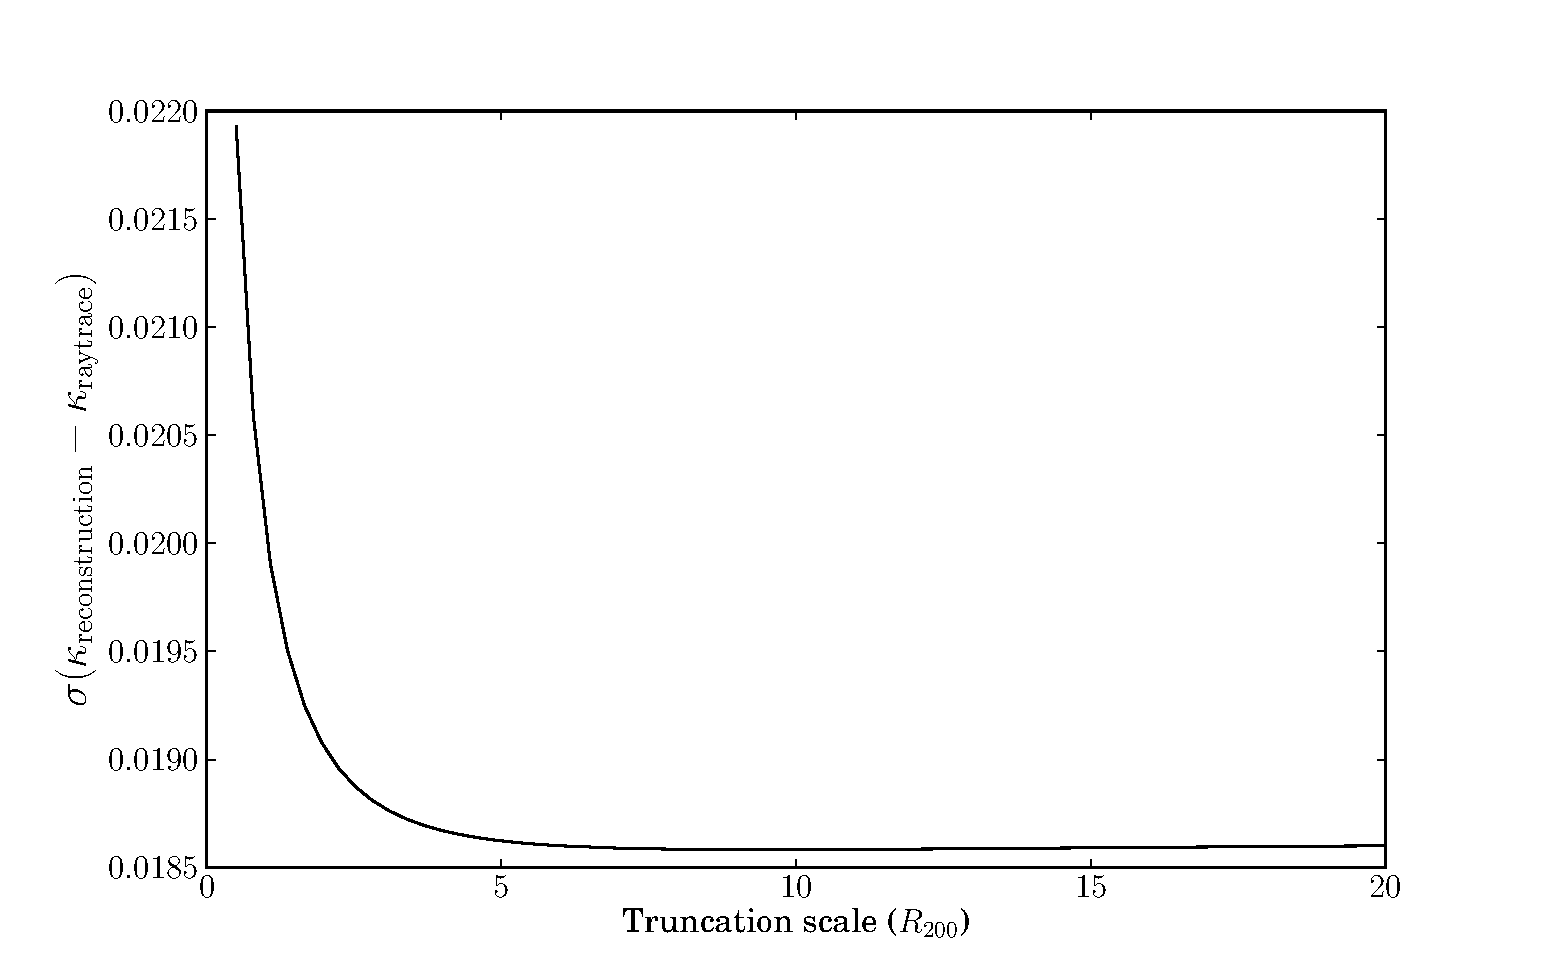
\includegraphics[width=\columnwidth]{figs/truncation_scatter.eps}
\caption[magcut]{The standard deviation in $\kapparec$ minus $\kapparay$ as a function of halo truncation radius in virial radii, using the truncated NFW profile of \citet{BMO}. In our models we truncate our halos at 5$R_{200}$}
\label{fig:ScattervsTruncation}
\end{figure}

For $\sumkappah$ to provide useful constraints on $\kapparay$, it is important that $\kapparay$ and $\sumkappah$ are as similar as possible. Figure \ref{fig:bias} shows that indeed $\sumkappah$ is a good estimator, regardless of the individual value of $\sumkappah$. At fixed $\sumkappah$ we find that the scatter in $\kapparay$ grows with $\sumkappah$; our reconstruction is better at reproducing underdense lines of sight than overdense lines of sight.

\begin{figure}
% 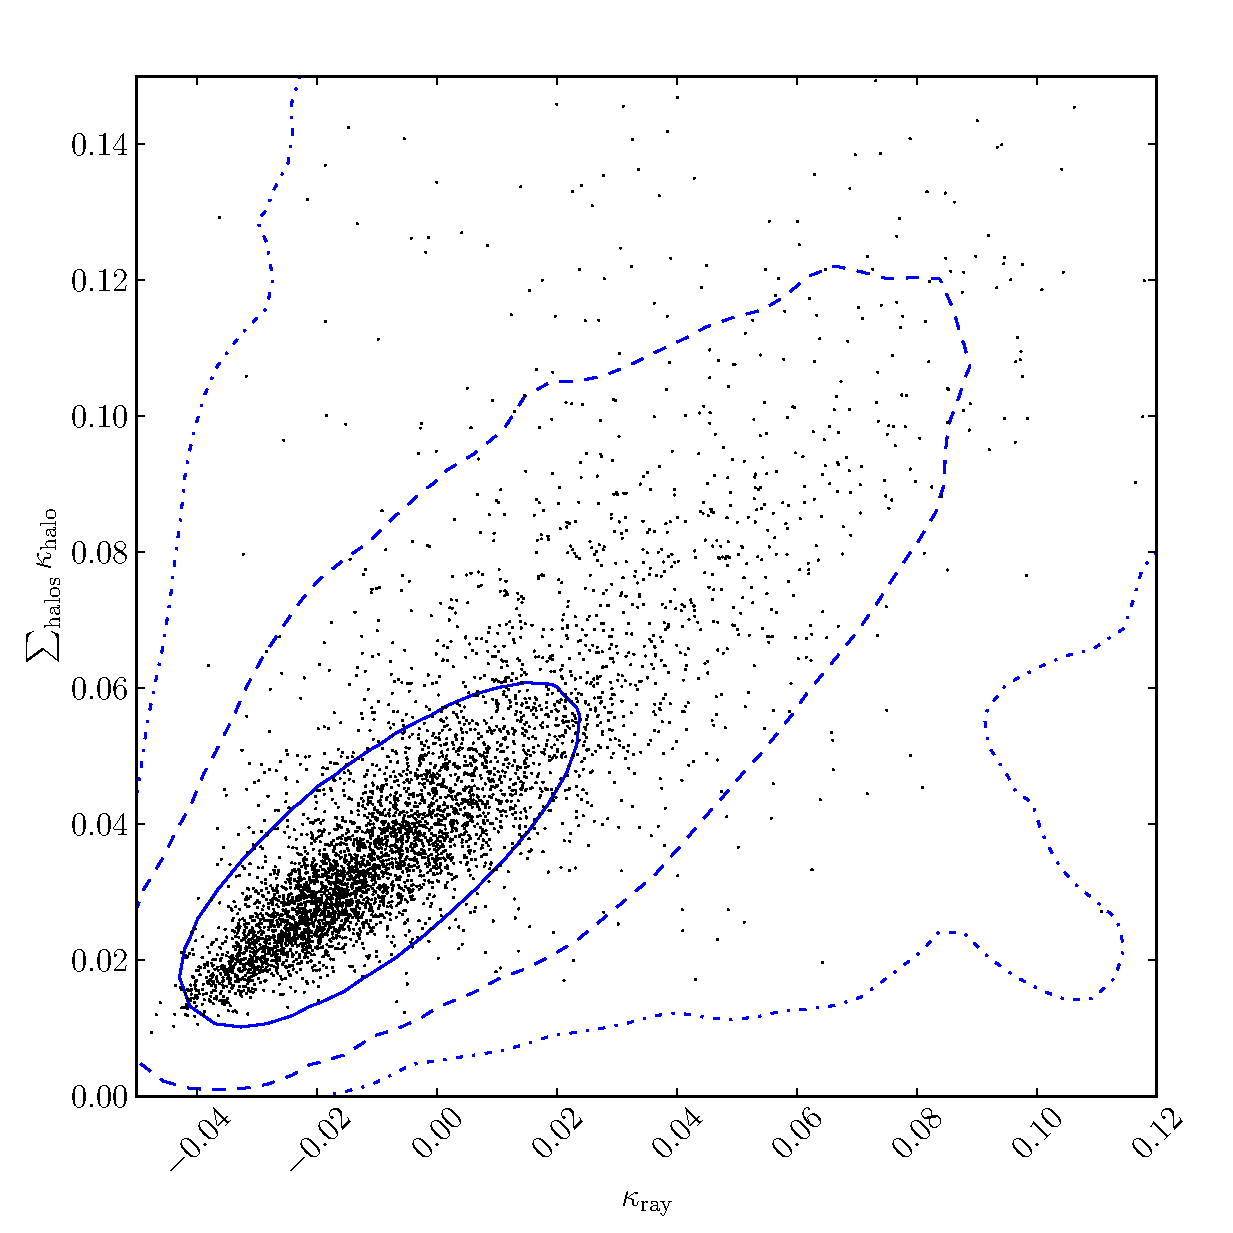
\includegraphics[width=\columnwidth]{figs/perfectc.eps}
\caption[Biased?]{$\sumkappah$ verses $\kapparay$ for 100000 reconstructed lines of sight. $\sumkappah$ traces $\kapparay$, but with a non-zero offset which is due to the negative connvergence from voids. At fixed $\sumkappah$ the scatter in $\kapparay$ grows with $\sumkappah$.}
\label{fig:isitbiased}
\end{figure}

The intrinsic error between the results of the halo based prescription and the raytraced convergence is an unavoidable error, even with perfect knowledge of halo mass and position. Before investigating the errors caused by imperfect knowledge of halo mass and redshift, we investigate the errors induced by a magnitude limited reconstruction and a field of view limited reconstruction. The halos in our catalogue are given magnitudes by the semi-analytic model of \citet{deLucia+Blaizot2007} and by applying magnitude cuts to our catalogue, we can investigate the scatter caused by unobserved halos. The majority of the convergence comes from halos with an $i$ magnitude between 18 and 24. Figure \ref{fig:magcut} shows that the width of $\kapparec-\kapparay$ decreases quickly between $i=18$ and $i=24$. Objects brighter than $i=18$ are either too rare or too close to the observer to make a significant contribution to the convergence. Objects fainter than $i=24$ are too small to be important, unless they are extremely close to the line of sight where it is likely that neglecting stellar mass and using a spherical NFW prescription are too naive to adequately reconstruct $\kappax$. It is likely that ultra-faint halos (or substructures), the uncertain contribution of voids and halos deviating from our spherical truncated NFW profile are the three major sources of the scatter in $\kapparec-\kapparay$; a deeper survey will not be sufficient to decrease the size of this scatter. Since a large number of callibration lines of sight must be reconstructed to sample $\pr(\kappav)$, it may prove unrealistic to reconstruct the calibration lines of sight out to 5 arcminutes. Figure \ref{fig:radcut} shows the width of $\kapparec-\kapparay$ as a function of reconstruction radius; in almost all cases there is no significant contribution to $\kappa$ from halos that are centred more than 1 arcminute away, although large groups or clusters can sometimes still make a contribution as far out as four arcminutes. For the rest of this work we will continue to model all of the halos out to 5 arminutes with an $i$ magnitude greater than 26, although a reconstruction with fields going out to two arcminutes and down to $i=24$ would do almost as well.

\begin{figure}
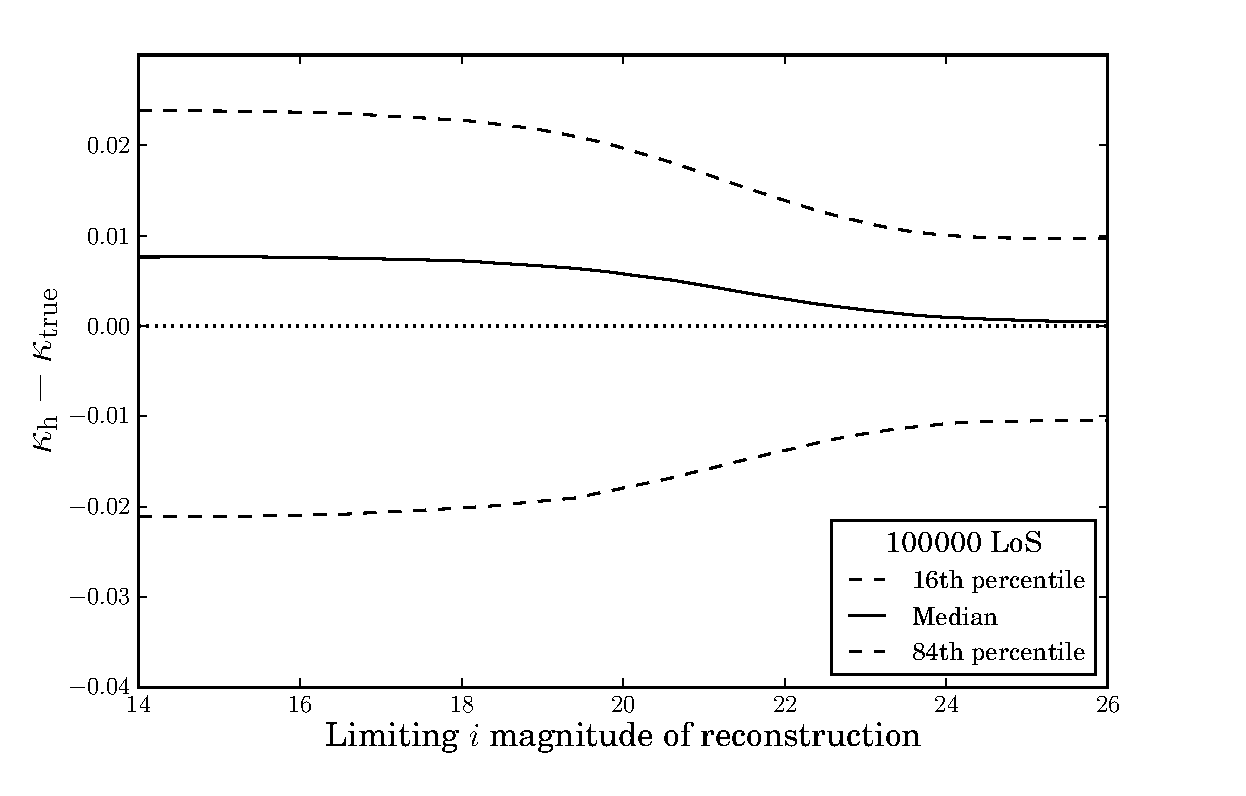
\includegraphics[width=\columnwidth]{figs/mag_scatter.eps}
\caption[magcut]{The 16, 50 and 84\% confidence intervals on $\kapparec$ minus $\kapparay$ as a function of the limiting $i$ band depth of the halo reconstruction. $\kapparec$ is given by $\sumkappah-\kappav$, where $\kappav$ is a constant such that $\left\langle\kapparec\right\rangle=0$. The majority of the constraining power comes from reconstructing halos with magnitudes between $18<i<24$}
\label{fig:magcut}
\end{figure}
\begin{figure}
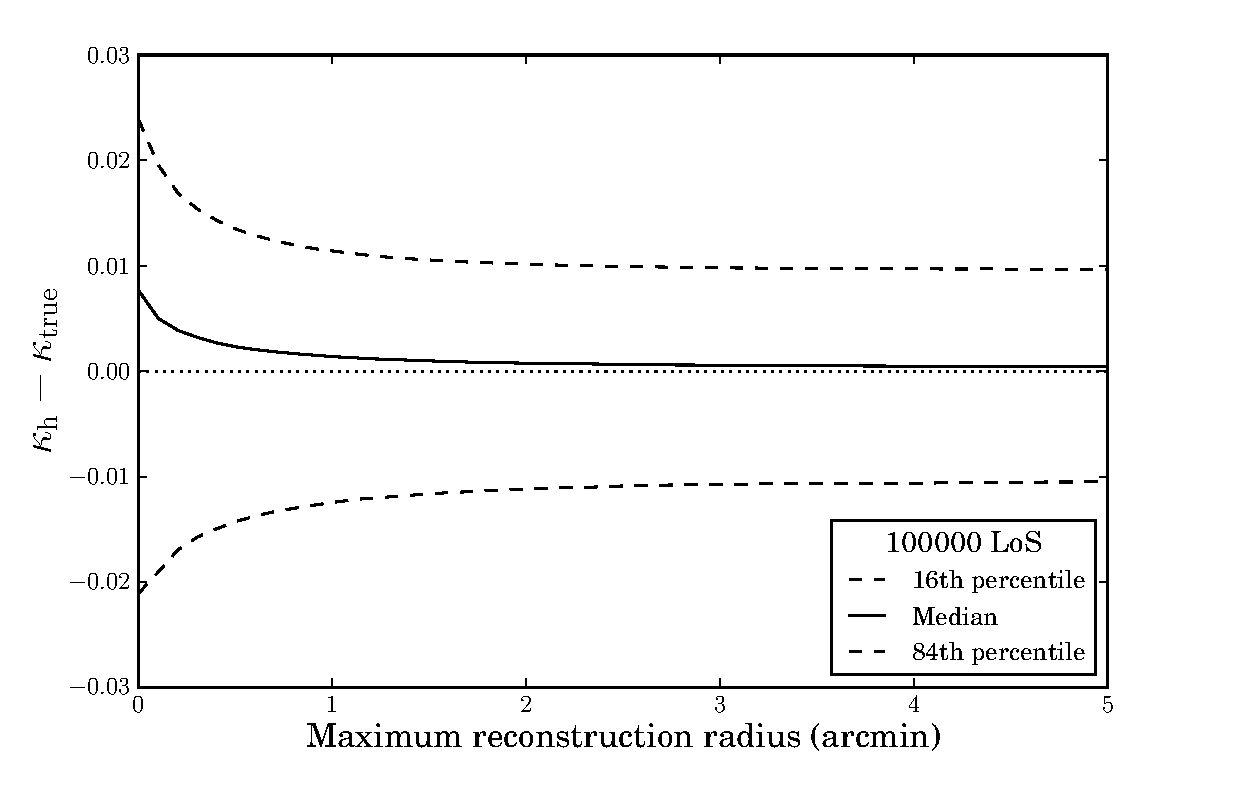
\includegraphics[width=\columnwidth]{figs/radius_scatter.eps}
\caption[radius cut]{The 16, 50 and 84\% confidence intervals on $\kapparec$ minus $\kapparay$ as a function of the limiting radius (in arcminutes) beyond which halos are not reconstructed. The majority of the convergence comes from halos centred within an arcminute of the line of sight}
\label{fig:radcut}
\end{figure}

The final test that we apply to the perfect knowledge reconstruction is to apply the marginalization outlined in Section \ref{subsec:voids}. Taking the reconstructed $\sumkappah$ for $1\times 10^{5}$ lines of sight we form the joint distribution, P$(\kapparay,\sumkappah)$ and marginalize over all sightlines with a similar $\sumkappah$ to give P($\kappax$). We define the bias as the difference between the expectation value of $\kappax$ and the known true value of $\kapparay$ for each Line of sight and we define the reconstruction width as half the width of the interval containing the central $68\%$ of the probability P($\kappax$). From $1\times 10^{4}$ reconstructed lines of sight we find the the bias to have mean of $-9.5\times 10^{-6}$ and a mean reconstruction width of 0.0132. In the case where one assumes P$(\kappax)$ is given by the global P$^{\rm global}(\kappax)$, the same $1\times 10^{5}$ lines of sight show a mean bias of $4.3\times 10^{-5}$ and mean reconstruction width of 0.237. Within the statistical error both methods are unbiased, but for any individual line of sight the bias is typically 1.8 times smaller with the reconstructed P$^{\rm reconstruction}(\kappax)$, rather than global P$^{\rm global}(\kappax)$. 

%%%%%%%%%%%%%%%%%%%%%%%%%%%%%%%%%%%%%%%%%%%%%%%%%%%%%%%%%%%%%%%%%%%%%%%%%%%%%%%%

\section{Applying the Halo Model approximation to mock catalogs}
\label{sec:obsMstar+z}

Real attempts to reconstruct the convergence along a line of sight will not have direct access to the masses of dark matter halos, 
and will likely not have access to their spectroscopic redshift either. Instead these properties must be inferred from astrophysical
observables. In principle the only observables are astrometric positions, photometric colours and possibly spectra. In this section we
quantify the errors induced by inferring the halo mass and redshift from the observables. Much work has already focused on using
photometric colours to infer stellar mass \citep[\eg][]{xxx} and redshifts \citep[\eg][]{BPZ}, in line with these we shall use
stellar mass and photometric redshifts (with appropriate errors), as the observables that must be converted into an estimate
of $\kappax$. We will investigate two main sources of error: inferring halo mass given observed stellar mass and placing halos at the wrong redshift due to photometric redshift error.

We generate a stellar mass for each halo according to the stellar mass--halo mass relation of \citet{BehrooziEtal2010}. From this stellar mass we simulate 
an observed stellar mass by drawing a sample from $\pr(\log(M_{* \mathrm {obs}})|\log(M_{* \mathrm {true}}))$ which is given by \comments{ the product of the galaxy stellar mass function (GSMF) of \citet{Fontana2006} and} a Gaussian of width $\sigma_{M_*}$ centred on $\log(M*_{\mathrm {true}})$. Where a spectroscopic redshift exists stellar masses can be estimated with typical uncertainties of 0.15 dex \citep{xxx}, however with photometric redshifts stellar mass uncertainties are typically three times as large \citep{xxx}; we use $\sigma_{M_*}=0.15$ for halos with a spectroscopic redshift and $\sigma_{M_*}=0.45$ otherwise. \comments{The \citet{Fontana2006} GSMF is given by a Schechter function with redshift evolving parameters
\be
\label{eq:GSMF}
{\dee N \over \dee M_*} \propto \left(10^{(M_*-M_0(z))}\right)^{(1+\alpha(z))} \exp \left(-10^{(M_*-M_0(z))}\right)
\ee 
where $M_0(z)=11.16+0.17z-0.07z^2$ and $\alpha(z)=-1.18-0.082z$.} For photometric redshift errors we draw a redshift from $\pr(z_{\rm true}|z_{\rm obs})$ which we take as a Gaussian of width $0.1(1+z_{\rm spec})$ centred on $z_{\rm spec}$, where $z_{\rm spec}$ is the halo's true redshift in the \MS catalogue

For each  source of error, we reconstruct 40000 calibration lines of sight and 10000 mock lens lines of sight, following the proceedure outlined in Section \ref{sec:model}. Reconstructing the lines of sight with perfect knowledge of the redshift but an uncertain stellar mass, we find that the width of $\Pr\left(\sumkappah \right)$ grows with the expectation value of $\sumkappah$; this is not surprising since the low $\sumkappah$ lines of sight are relatively empty and so there are few opportunities for uncertainties in the halo masses to propogate into $\sumkappah$ uncertainties. After applying the void correction the expected bias from our 10000 mock lenses is $6.7\times 10^{-5}$ and the mean reconstruction width is 0.0145; this is the typical reconstruction error that could be expected from a complete spectroscopic survey of the field, it is ten percent worse than the reconstruction given perfect knowledge of the halo masses and redshifts but still 1.6 times better than using the global P$^{\rm global}(\kappax)$ although a complete spetroscopic survey is still unrealistic. The distribution of the widths of $\Pr\left(\kappax \right)$ is shown in Figure \ref{fig:width1}


\begin{figure}
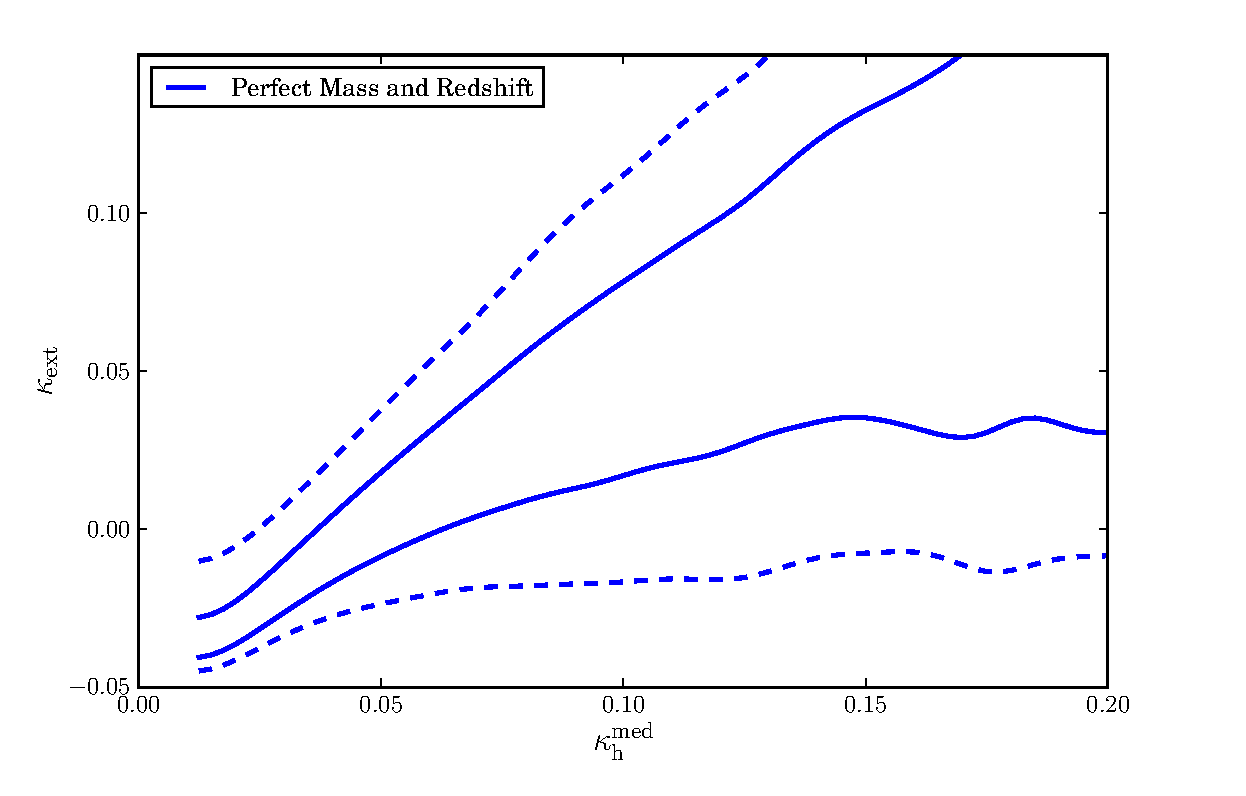
\includegraphics[width=\columnwidth]{figs/cornerplot.eps}
\caption{68 \% and 95 \% contours of the joint distribution $\pr(\kapparay, \tilde\kappa_{\rm halos})$ given a mock reconstruction of our 40000 calibration lines of sight. $\tilde\kappa_{\rm halos}$ is the median of $\pr(\sumkappah)$ given a spectroscopic redshift for each halo. $\kapparay$ and $\tilde\kappa_{\rm halos}$ are strongly correlated, despite the blurring effect of uncertain halo masses.}
\label{fig:corner}
\end{figure}

\begin{figure}
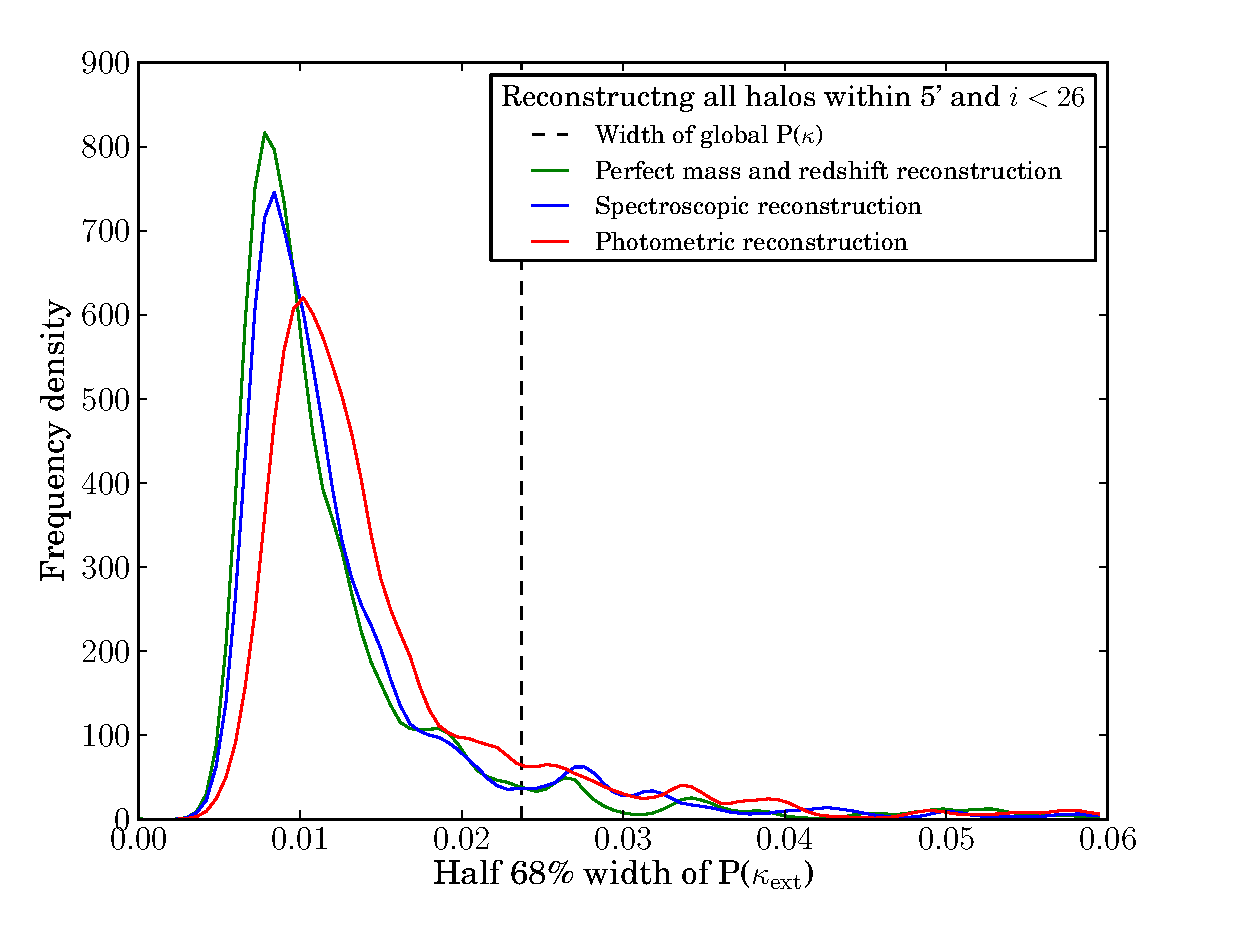
\includegraphics[width=\columnwidth]{figs/widths.eps}
\caption{Widths of $\pr(\kappax)$ after applying our reconstruction of all halos down $to i=26$ and within 5 arcminutes of the line of sight. Results for 10000 lines of sight are shown. Green is for a reconstruction given perfect knowledge of halo mass and redshift, blue is for a reconstruction given a spectroscopic redshift for every halo, and red is for a reconstruction with photometric redshifts only. The dashed black line shows the width of the global $\pr(\kappax)$ distribution; the reconstruction process provides roughly a factor of 2 improvement for the majority of lines of sight. Spectroscopic redshifts improve the reconstruction, but at signifcant observational cost.}
\label{fig:width1}
\end{figure}

Inferring the stellar mass of a galaxy from its magnitude and colours requires an estimate of how far away the galaxy is; without a spectroscopic redshift the the infered stellar mass is less precise. In principle the photometric redshift is correlated with the infered stellar mass, however we do not model this effect since the convergence from the outskirts of an individual halo is only weakly dependant on redshift at fixed mass: the redshift error is small effect on the recovered $\pr(\kappa)$ when compared to the effect of uncertain stellar masses.  With only photometric redshifts the uncertainty on $\sum\kapparec^{\rm halos}$ is much larger than the spectrocopic case, but this does not propogate into a much larger bias after applying the void correction; with a purely photometric reconstruction of the 10000 mock lightcones the results have a mean bias of $1.1\times 10^{-4}$ and a mean width of 0.0158. On average a purely photometric reconstruction of the field gives an unbiased $\pr(\kappax)$ that is 1.5 times tighter than assuming the global $\pr^{\rm global}(\kappax)$. 


%\subsection{Reconstructions of Smaller and Shallower Fields}

\begin{figure}
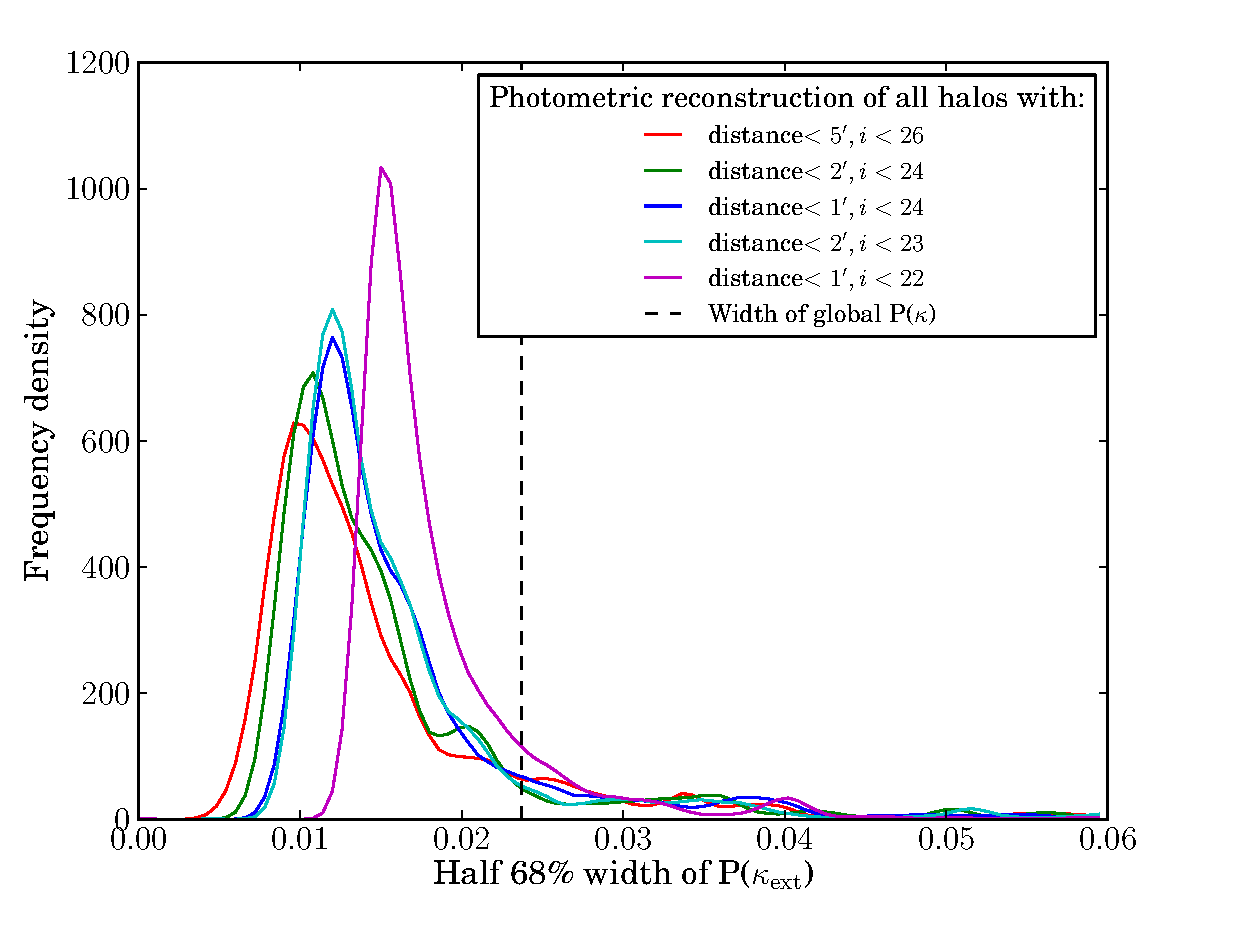
\includegraphics[width=\columnwidth]{figs/widths2.eps}
\caption{Widths of $\pr(\kappax)$ after a photometric reconstruction of all halos within different fields. The different field sizes and depths are given in the legend. As the field becomes smaller or shallower, fewer halos are being reconstructed and so the width of $\pr(\kappax)$ grows.}
\label{fig:width2}
\end{figure}


Reconstructions of real lines of sight may not have access to the deep, large calibration fields that we have used upto this point. We can perform the same reconstruction but for a more modest mock survey. Given the results of Section \ref{sec:knownMh+z} we predicted that a reconstruction of the field out to 2 arcminutes and a magnitude limit of $i$=24 would provide similar constraints to a reconstruction going out to 5 arcminutes and going down to $i$=26. We find the mean reconstruction width to be 0.0163 for a photometric reconstruction of all the halos within 2 arcminutes that have $i<24$, this is only marginally worse than 0.0158 which was the typical width after the deeper and wider reconstruction of the previous section. The reconstruction widths for our 10000 mock lens lines of sight are shown in Figure \ref{fig:widths2}. If only photometry for halos with $i<24$ and within 1 arcminute of the line of sight is availble then the typical width of the reconstructed $\pr(\kappax)$ is 0.173. Whilst a complete spectroscopic survey of a large field would be unlikely, a hybrid strategy of obtaining spectra for a subset of objects may be feasible. Photometric redshifts are sufficient to asertain the halos which are likely to contribute most of the convergence on any given line of sight, and on average there are only $\sim 6 \pm 6$ halos per line of sight that individually contribute more than 0.002 to $\sumkappah$. We investigate a hybrid strategy of obtaining spectroscopic redshifts for all of the $i<24$ halos which contribute an individual $\kappa$ of at least 0.002 combined with a photometric redshift for all other $i<24$ halos within 2 arcminutes. For the hybrid strategy the typical width of the reconstructed $\pr(\kappax)$ is 0.0151. The observational cost of obtaining spectroscopic redshifts for several 24th magnitude galaxies may make the hybrid strategy unlikley, but obtaining photometry of a 4$\times$4 arcminute patch of sky down to $i=24$ is fast with modern telescopes. The mean reconstruction width for a photometric reconstruction of all the halos within 2 arcminutes that have $i<24$ represents an improvement of 1.5 over using the global $\pr(\kappax)$ and should be achievable at minimal observational cost.


%%%%%%%%%%%%%%%%%%%%%%%%%%%%%%%%%%%%%%%%%%%%%%%%%%%%%%%%%%%%%%%%%%%%%%%%%%%%%%


\section{Testing for Systematic errors}
\subsection{Using the wrong M$_{\rm halo}$-M$_{*}$ relation}
\subsection{Selecting bias from a subset of lines of sight?}
\subsubsection{Selecting only the lines of sight with tight $\pr(\kappax)$}
\subsubsection{Selecting only high shear lines of sight}

%%%%%%%%%%%%%%%%%%%%%%%%%%%%%%%%%%%%%%%%%%%%%%%%%%%%%%%%%%%%%%%%%%%%%%%%%%%%%%
\comments{

\subsection{Comparison with Other Treatments of $\kappax$}
\label{sec:Dt:selection} 

\phil{How does distance accuracy compare with simple averaging? eg assuming
$\kappax = 0$ for all lenses. How does it compare with the no data situation?
eg where the intrinsic distribution of kappa is used as $Pr(\kappax)$.}

What is the expected bias and scatter (centroid position and width) of P(D) as a
function of N lenses? How does reconstruction compare with P(D) derived using
P(kappa|N45) for each lightcone? How does reconstruction compare with P(D)
derived assuming kappa=0 for each lightcone?

Also: compare with simple averaging. This will fail if lenses are selected to
live on over-dense lines of sight. Stefan's plot in Suyu et al shows effect of
selection - what is the resulting bias? Few percent? This is the target to beat,
need to find it out.

\subsection{Improving the Accuracy with More Information}
\label{sec:Dt:selection} 

\phil{How does distance accuracy improve with:}
\begin{itemize}
\item Spectroscopic coverage? For galaxies above some mlim? For targets with
high kappa contribution (based on photometry)?
\item IR coverage for all objects? Improves photo-z and Mstar.
\item Including shear information from lens model? Assume accurate but
uncertain extertanl shear.
\end{itemize}
}
%%%%%%%%%%%%%%%%%%%%%%%%%%%%%%%%%%%%%%%%%%%%%%%%%%%%%%%%%%%%%%%%%%%%%%%%%%%%%%

\section{Discussion}
\label{sec:discuss}

We have shown that reconstructing the matter due to halos along any line of sight can give meaningful and unbiased constraints on the external convergence along that line of sight. The total convergence along a line of sight is strongly correlated with the reconstructed $\sumkappah$. However since our model ignores voids and assumes all halos follow a spherical truncated-NFW profile our model does not include all of the relevant physics, hence the width of our resulting $\pr(\kappax)$ is still typically $\sim$0.01, even with a perfect knowledge of every halo's virial mass and redshift. To make further progress a more advanced treatment of both voids and halos will be necessary. Interestingly, we have found that the most empty lines of sight can be reconstructed with the most precision. $\kappax$ for empty lines of sight have little contributions from halos and a large contribution from voids; since they have the tightest PDFs after the reconstruction it seems that our model's biggest uncertainties are driven by naively reconstructing halos rather than neglecting voids. With a photometric reconstruction of the field there is only a small broadening compared to the perfect knowledge reconstruction; it seems that deviations from sphericity and dark matter clumping within the main halo are the dominant uncertainies rather than uncertainties in the halo mass. Inferring halo ellipticity and dark matter clumping will likely always remain a difficulty for line of sight reconstruction; as Figures \ref{fig:magcut} and \ref{fig:width2} show observing deeper than 24th magnitude does not signifcantly help the reconstruction. Because our reconstruction is mostly limited by the model, spectroscopic coverage can only provide a modest improvement to the reconstruction and at significant observational cost.

For a small fraction of lines of sight, $\pr(\kappax)$ remains very broad even after applying our reconstruction; these lines of sight are typically the most overdense lines of sight in the universe. For time-delay cosmography the most observationally expensive task is the lightcurve monitoring, whilst making photometric observations of a 4$\times$4 arcminute patch of sky survey down to 24th magnitude is a relatively cheap. We have shown that with a single epoch observation of the region around a strong lens it is possible to infer $\pr(\kappax)$. If a line of sight has a broad $\pr(\kappax)$ it can be rejected {\it before} the investment of longterm lightcurve monitoring.

The method we have outlined can also be used to estimate the external shear
along a line of sight. Shear is an observable that can be extracted from
strong lens modelling, however there is a degeneracy between internal and
external shear. Progress has been made in disentangelling external and
internal shear \citep[\eg][]{xxx} but there are still significant
uncertainties: \citet{WongEtal2011} attempted to match the shear from strong
lens models with a reconstruction of the local lens group environment, but
found a tension between the strong lens model and the reconstruction of the
environment. Since \citet{WongEtal2011} only reconstructed the local lens
group, rather than the full line of sight contribution, it is unclear whether
the external shear from lens models can be reconciled with a line of sight
reconstruction. {\it If} external shear can be measured, it provides an
additional constraint on which of the Millenium Simulation lines of sight are
similar to the reconstructed line of sight. \citet{SuyuEtal2012} found that
for RXJ1131 combining shear constriants with galaxy number count overdensity,
gave a significantly different $\pr(\kappax|\gamma,N_{45})$ copmpared to the
PDFfrom number count overdensity alone, $\pr(\kappax|N_{45})$. 



%%%%%%%%%%%%%%%%%%%%%%%%%%%%%%%%%%%%%%%%%%%%%%%%%%%%%%%%%%%%%%%%%%%%%%%%%%%%%%

\section{Conclusions}
\label{sec:conclude}

In this work we have investigated a simple halo model prescription for
reconstructing all the mass along a line of sight to an intermediate redshift
source. We have used the ray-traced lensing convergence along lines of sight
through the Millenium Simulation to test this approach, and to calibrate
estimates of the total convergence along a line of sight to an observed
distant galaxy made by summing the convergences due to each object in a
photometric catalogue. Having found that the reconstruction process is effective given perfect
knowledge of halo mass and redshift, we investigated the effects of reasonable
uncertainties in the stellar mass and redshift of each halo, and propogated
these uncertainties into a $\pr\left(\sumkappah\right)$ for each line of
sight. We draw the following conclusions:

\begin{itemize} 

\item Our model uses a truncated spherical NFW profile for
each dark matter halo and neglects voids, but despite the model's simplicity
the reconstructed $\sumkappah$ is a good tracer of $\kappax$.  We found that
with perfect knowledge of the halo mass and redshift (from the Millenium
Simulation catalogs), the reconstruction gives an unbiased estimate of
$\pr(\kappax)$ for a single line of sight that is almost almost a factor of 2
less broad than the global $\pr(\kappax)$. 

\item  For the most overdense lines of sight, the reconstruction produces a
very broad PDF, but since the reconstruction can be performed before follow-up
time is invested it will be possible to discard the most uncertain lines of
sight and prevent the waste of follow-up time. 

\item With complete spectroscopic redshift coverage and just an empirical
stellar mass to halo mass relation, we find that the median of
$\pr\left(\sumkappah\right)$ is a useful indicator for generating an estimate
of $\pr(\kappax)$ from the ensemble of simulated lines of sight. The resulting
PDF tends to be around 10\% broader than it would have been given perfect
knowledge of both halo mass and redshift; given only photometric redshifts
(which in turn give rise to much less certain stellar masss estimates) causes
another $\sim$10\% increase to the width of $\pr(\kappax)$.

\item It is very rare for halos further than 2 arcminutes to make a
significant contribution to $\kappax$. We also found that including halos
whose host galaxy is less luminous than $i=24$ does not significantly improve
our reconstruction proceedure. A photometric survey to this depth of a
4$\times$4 arcminute patch around the lens would approach the limiting
uncertainties of our simple reconstruction recipe, and yield a 
$\pr(\kappax)$ that has, on average, a width of 0.0163 --
50\% less broad than the global $\pr(\kappax)$.

\item We find that the lines of sight with the sharpest $\pr(\kappax)$ are
typically under-dense. With a photometric reconstruction of all lens fields,
and following up only the lenses with the most constraining $\pr(\kappax)$,
the width of the dominant statistical uncertainty in time-delay cosmography
can be halved, whilst at the same time decreasing any potentail for a
systematic error due to lenses being biased in $\kappax$.

\end{itemize}

\todo{Tom}{Add more conclusions about bias in a large sample of lenses...}

\todo{Tom}{Wrap up}


%Our conclusions can be summarised as follows:
%\begin{itemize}
%\item With perfect 
%\item And we found this too.
%\end{itemize}

% \item Faint galaxies and other dark structures will not appear in a photometric
% object catalog, but they will contribute convergence at some level. How much of
% the total external convergence in a time delay lens system comes from visible
% galaxies? How does this change as a function of magnitude cut? 

% \item Can the true (ray-traced) convergence be recovered by halo model
% reconstruction, and with what scatter and residual bias? Which aspects of the 
% model dominate these uncertainties?

% \item When faced with a newly-detected lens, surrounded by galaxies on the sky,
% we have some choices to make when planning follow-up observations.
% Which are the most important galaxies, with regard to the external convergence
% produced? Can nearby groups and clusters be straightforwardly accounted for? If
% lenses with such massive structures nearby are discarded, what impact does that
% have on the distance accuracy?



%%%%%%%%%%%%%%%%%%%%%%%%%%%%%%%%%%%%%%%%%%%%%%%%%%%%%%%%%%%%%%%%%%%%%%%%
%%  ACKNOWLEDGMENTS
%%%%%%%%%%%%%%%%%%%%%%%%%%%%%%%%%%%%%%%%%%%%%%%%%%%%%%%%%%%%%%%%%%%%%%%%

\section*{Acknowledgments}
 
TC thanks Vasily Belokurov for guidance and discussions.
We thank Risa Wechsler and Peter Behroozi for useful discussions and 
suggestions.
TEC acknowledges support from STFC in the form of a research studentship.
%
PJM was given support by the Kavli Foundation and the Royal 
Society, in the form of research fellowships.
%
MWA \ldots
%
SH \ldots
%
SHS \ldots
%
TT acknowledges support from the NSF through CAREER award NSF-0642621,
and from the Packard Foundation through a Packard Research Fellowship.
% 
LVEK acknowledges the support by an NWO-VIDI programme subsidy
(programme number 639.042.505).
%
This research is supported in part by the National Science Foundation under
Grant No. PHY99-07949.



%%%%%%%%%%%%%%%%%%%%%%%%%%%%%%%%%%%%%%%%%%%%%%%%%%%%%%%%%%%%%%%%%%%%%%%%%%%%%%
%  APPENDICES
%%%%%%%%%%%%%%%%%%%%%%%%%%%%%%%%%%%%%%%%%%%%%%%%%%%%%%%%%%%%%%%%%%%%%%%%%%%%%%

\appendix

%%%%%%%%%%%%%%%%%%%%%%%%%%%%%%%%%%%%%%%%%%%%%%%%%%%%%%%%%%%%%%%%%%%%%%%%%%%%%%

\section{Truncated NFW halos}
\label{appendix:halos}

 Defining $x$ as the dimensionless projected radial distance $R/r_{s}$ and $\tau$ as the dimensionless truncation radius $r_{t}/r_{s}$, \citet{BMO} derives the projected mass density, which is given by:
\begin{align}\label{eq:kappaBMO}
\Sigma_{\rm}(x) = {2\tau^2 \over (\tau^2+1)^2}\left(
        {\tau^2+1\over x^2-1}\left(1-\mathcal{F}(x)\right)
        +
        2\mathcal{F}(x)\right.\nonumber\\
        -
        \left. {\pi \over \sqrt{\tau^2+x^2}}
        +
        {(\tau^2-1)\mathcal{L}(x,\tau)
        \over
        \tau\sqrt{\tau^2+x^2}}\right)
\end{align}
where $\mathcal{F}(x)$ and $\mathcal{L}(x,\tau)$ are defined as
\be\label{eq:F} 
\mathcal{F}(x) \equiv \begin{cases}  \frac{{\rm cos}^{-1} (1/x)}{\sqrt{x^2-1}} \hspace{0.2cm} & (x>1) \\
\\
\frac{4-x^2}{3}  & (x=1)\\
\\
\frac{ {\rm cosh}^{-1} (1/x)}{\sqrt{1-x^2}} & (x<1)
\end{cases}
\ee
\be\label{eq:L}
\mathcal{L}(x,\tau) = \ln\left(\frac{x}{\sqrt{\tau^2+x^2}+\tau}\right)
\ee
%the convergence is given by $\Sigma_{\rm BMO}(x) / \Sigma_{\rm cr}(z)$.



%%%%%%%%%%%%%%%%%%%%%%%%%%%%%%%%%%%%%%%%%%%%%%%%%%%%%%%%%%%%%%%%%%%%%%%%%%%%%%

\section{Inferring $\Mhalo$ given a noisy measurement of $\Mstarobs$}
\label{appendix:MSMH}

Given a noisy estimate of the stellar mass $\Mstarobs$ of a galaxy at redshift
$z$, how can we infer the galaxy's halo mass? We then seek the posterior
PDF $\Pr(\Mhalo|\Mstarobs)$, which can be expanded as follows:

\begin{eqnarray}
&& \Pr(\Mhalo|\Mstarobs,z) = \notag\\
&& \int d\Mstar \Pr(\Mhalo|\Mstar,z) \Pr(\Mstar|\Mstarobs,z), \notag\\
&\propto& \int d\Mstar \Pr(\Mstarobs|\Mstar) \Pr(\Mstar|\Mhalo,z) \Pr(\Mhalo|z),
\label{eq:mhalo-mstar}
\end{eqnarray}
where we have used Bayes' Theorem twice to replace
$\Pr(\Mhalo|\Mstar,z) \Pr(\Mstar|z)$ with 
$\Pr(\Mstar|\Mhalo,z) \Pr(\Mhalo|z)$, and 
to invert $\Pr(\Mstar|\Mstarobs)$ into the sampling
distribution $\Pr(\Mstar|\Mstarobs)$, which we recognise as the likelihood
function for the observed stellar mass. Note that the ``true'' $\Mstar$ of the
galaxy is marginalised out: we are only interested in reconstructing the halo
mass. The last two terms in
\eqref{eq:mhalo-mstar} are the $\Mstar-\Mhalo$ relation from
\citet{BehrooziEtal2010}, and the halo mass function $\Pr(\Mhalo|z)$, at the
given redshift. We can
tabulate the product of these two from our Millenium Simulation catalog,
constructing a two-dimensional histogram of halo masses and their associated
true stellar masses (drawn from the Behroozi relation). 

For each galaxy, we compute the likelihood function for its $\Mstarobs$ as a
function of the unknown $\Mstar$, and multiply it by our tabulated joint PDF.
This heavily downweights halos with $\Mstar$ values outside the observed
range. We then do the marginalisation integral by Monte Carlo, drawing
(two-dimensional) sample parameter vectors
from the downweighted histogram, discarding the $\Mstar$ values, and
constructing a one-dimensional histogram that is an estimate of
$\Pr(\Mhalo|\Mstarobs)$.

\todo{Matt}{Edit the above text to add a note on how we do the sampling in
practice, via the CDF.}

If the redshift of the galaxy is uncertain, we need to take this uncertainty
into account; for example, for each sample drawn from the photometric redshift
posterior PDF $\Pr(z|{\rm colors})$, we can draw a sample $\Mhalo$ using the
above procedure.


%%%%%%%%%%%%%%%%%%%%%%%%%%%%%%%%%%%%%%%%%%%%%%%%%%%%%%%%%%%%%%%%%%%%%%%%%%%%%%

\section{Accounting for uncatalogued low mass halos, and voids}
\label{appendix:smooth}

Our halo model allows us to infer a halo mass $\Mhalo$ for each galaxy in a
photometric catalog; under the weak lensing approximation described in
\Sref{sec:theory} we can compute the contribution of each of these halos to
the overall convergence and shear amplitude, assuming a homogeneous
Friedman-Robertson-Walker metric and the concordance $\Lambda$CDM cosmological
parameters for the angular diameter distances to calculate the critical
density for each lens plane. Clearly this approach will tend to over-estimate
the convergence, since we are placing massive halos into a volume that has
already been assumed to be full of homogeneously distributed matter with the 
mean cosmological density. In practice, the space between massive halos will
contain a) low mass halos that are not bright enough to be detected and b)
empty space where the density is below that of the mean. A rigorous treatment
of this complex situation is beyond the scope of this paper, but is being
investigated (Blandford et al, in preparation). In this appendix we describe
our empirical approach to accounting for the missing mass and voids. 

Let the summed convergence due to halos in our galaxy catalog be $\kappah$.
Given some assumptions about halo density profile and shape, this parameter
can be inferred from a set of uncertain halo mass estimates (which have in
turn been inferred from noisy measurements of galaxy redshift and stellar mass
as described in \Aref{appendix:MSMH}). We assume each halo to be a
spherically-symmetric NFW profile, and neglect the contribution of the stellar
mass to the convergence. The halo mass inference for the $k^{\rm th}$ galaxy 
is stored as a list of sample values of $\Mhalok$ drawn from the posterior PDF
$\Pr(\Mhalok|\Mstarobsk,z_k)$; computing the contribution to the convergence
due to this halo at the target line of sight for each sample gives, in turn, 
a set of
samples drawn from the PDF $\Pr(\kappahk|\Mstarobsk,z_k)$. We then generate
samples from $\Pr(\kappah|\{\Mstarobsk,z_k\})$ by drawing a sample $\kappahk$
for each halo, summing over halos to get $\kappah$, discarding those
samples and moving down the lists.

The PDF $\Pr(\kappah|\{\Mstarobsk,z_k\})$ will, in general, be broad (due to
the uncertainties involved in halo mass estimation). It will also be shifted
towards high values of convergence, due to the FRW approximation described
above. What we really want is an inference of $\Pr(\kappa|\{\Mstarobsk,z_k\})$
instead. We can obtain this by considering the expansion:
\begin{equation}
\Pr(\kappa|\{\Mstarobsk,z_k\}) = \int d\kappah 
   \Pr(\kappa|\kappah) \Pr(\kappah|\{\Mstarobsk,z_k\})
\label{eq:kappaconv}   
\end{equation}
The first term in the integrand relates the summed  convergence due to model
halos, $\kappah$, to the true summed convergence, $\kappa$.  In the Millenium
Simulation catalogs, we can compute a single value of $\kappah$ for each
selected line of sight from the true halo mass and redshift (and our same
assumptions of halo profile and shape), and tabulate the two-dimensional PDF
$\Pr(\kappa|\kappah)$ as a sequence of one-dimensional PDFs for $\kappa$ in a
bin at fixed $\kappah$. Note that this PDF captures the ``intrinsic scatter''
of $\kappah$ due to our assumptions about the clumpiness of mass in the
Universe; the integral combines these uncertainties with those
arising from the measurement of $\Mstarobs$ and~$z$.

For any given observed catalog then, we infer
$\Pr(\kappah|\{\Mstarobsk,z_k\})$ as described above, and then
multiply it by $\Pr(\kappa|\kappah)$; we
again do the marginalisation over $\kappah$ by Monte Carlo, drawing samples
from the two-dimensional grid and keeping only the $\kappa$ values, to form
our final result, $\Pr(\kappa|\{\Mstarobsk,z_k\})$. 
This PDF will describe, by construction, an accurate (i.e., unbiased)
measurement of $\kappa$ in the case where the Millenium Simulation halo
catalog and Behroozi et al $\Mstar-\Mhalo$ relation are themselves accurate
descriptions of galaxies and their distribution. In \Sref{sec:tests} we
investigate the amplitude of the systematic errors incurred if these
assumptions are not valid.

\todo{Matt}{Add text describing whatever sampling shortcut you derive! :-)}

% Finally, we note that \Eref{eq:kappaconv} and the method for evaluating the
% integral in it can be generalized to yield 
% $\Pr(\kappa,|\gamma||\{\Mstarobsk,z_k\})$, where $|\gamma|$ is the amplitude
% of the complex shear. The amplitude of the shear due to halos, $|\gammah|$ is
% needed in this calculation, and marginalised over -- $\gammah$ is computed by
% simple summation of its components, as in \Sref{sec:theory}. In
% \Sref{sec:includinggamma} we explore the impact that knowing $\gamma$ (from,
% for example, a strong lens model)  has on the inference of $kappa$, and how
% severe the systematic errors from getting this wrong might be.


%%%%%%%%%%%%%%%%%%%%%%%%%%%%%%%%%%%%%%%%%%%%%%%%%%%%%%%%%%%%%%%%%%%%%%%%%%%%%%
%  REFERENCES
%%%%%%%%%%%%%%%%%%%%%%%%%%%%%%%%%%%%%%%%%%%%%%%%%%%%%%%%%%%%%%%%%%%%%%%%%%%%%%

% MNRAS does not use bibtex, input .bbl file instead. 
% Generate this in the makefile using bubble script in scriptutils:

% bubble -f paper-lcr.tex references.bib 
% %%%%%%%%%%%%%%%%%%%%%%%%%%%%%%%%%%%%%%%%%%%%%%%%%%%%%%%%%%%%%%%%%%%%%%%%
%
% Pangloss: Testing the reconstruction paper
%
%%%%%%%%%%%%%%%%%%%%%%%%%%%%%%%%%%%%%%%%%%%%%%%%%%%%%%%%%%%%%%%%%%%%%%%%

\documentclass[useAMS,usenatbib]{mn2e}
%% letterpaper
%% a4paper

% \voffset=-0.8in

% Packages:
\input psfig.sty
\usepackage{xspace}
\usepackage{graphicx}
\usepackage{amssymb}
\usepackage{amsmath}

% Macros:
% JOURNALS
\newcommand{\apj}{ApJ}
\newcommand{\apjl}{ApJL}
\newcommand{\apjs}{ApJS}
\newcommand{\mnras}{MNRAS}
\newcommand{\apss}{Ap \& SS}
\newcommand{\aap}{A\&A}
\newcommand{\aj}{AJ}
\newcommand{\prd}{Phys. Rev. D}
\newcommand{\nat}{Nature}
\newcommand{\araa}{ARA\&A}
\newcommand{\jgr}{J. Geophys. Res.}
\newcommand{\pasp}{PASP}

% MISC
\newcommand{\etal}{et~al.~}
\def\spose#1{\hbox  to 0pt{#1\hss}}  
\newcommand{\lta}{\mathrel{\spose{\lower 3pt\hbox{$\sim$}}\raise  2.0pt\hbox{$<$}}}
\newcommand{\gta}{\mathrel{\spose{\lower  3pt\hbox{$\sim$}}\raise 2.0pt\hbox{$>$}}}
\newcommand{\eg}{{\it e.g.\ }}
\newcommand{\ie}{{\it i.e.\ }}
\newcommand{\be}{\begin{equation}}
\newcommand{\ee}{\end{equation}}
\newcommand{\dee}{\, \mathrm{d} \!}
\newcommand{\bea}{\begin{eqnarray}}
\newcommand{\eea}{\end{eqnarray}}


% CROSS-REFERENCING
\def\Sref#1{Section~\ref{#1}\xspace}
\def\Fref#1{Figure~\ref{#1}\xspace}
\def\Tref#1{Table~\ref{#1}\xspace}
\def\Eref#1{Equation~\ref{#1}\xspace}
\def\Eqref#1{Eq.~(\ref{#1})\xspace}
\def\Aref#1{Appendix~\ref{#1}\xspace}

% UNITS
\newcommand{\kms}{\ifmmode  \,\rm km\,s^{-1} \else $\,\rm km\,s^{-1}  $ \fi }
\newcommand{\kpc}{\ifmmode  {\rm kpc}  \else ${\rm  kpc}$ \fi  }  
\newcommand{\pc}{\ifmmode  {\rm pc}  \else ${\rm pc}$ \fi  }  
\newcommand{\Msun}{\ifmmode {\rm M_{\odot}} \else ${\rm M_{\odot}}$ \fi} 
\newcommand{\Zsun}{\ifmmode {\rm Z_{\odot}} \else ${\rm Z_{\odot}}$ \fi} 
\newcommand{\yr}{\ifmmode yr^{-1} \else $yr^{-1}$ \fi} 
\newcommand{\hMsun}{\ifmmode h^{-1}\,\rm M_{\odot} \else $h^{-1}\,\rm M_{\odot}$ \fi}

% COSMOLOGY
\newcommand{\LCDM}{$\Lambda{\rm CDM}$}
\newcommand{\MS}{Millennium Simulation\xspace}

% LENSING
\def\zd{z_{\rm d}}
\def\zs{z_{\rm s}}
\def\Dd{D_{\rm d}}
\def\Ds{D_{\rm s}}

\def\Dt{D_{\Delta t}}

\def\Dds{D_{\rm ds}}
\def\Sigmacrit{\Sigma_{\rm crit}}
\def\REin{R_{\rm Ein}}
\def\MEin{M_{\rm Ein}}
\def\xkappa{\kappa_{\rm ext}}
\def\kappax{\kappa_{\rm ext}}
\def\kappaxtrue{\kappax^{\rm true}}
\def\kappah{\kappa_{\rm h}}
\def\kappav{\kappa_{\rm void}}
\def\kapparay{\kappa_{\rm raytrace}}
\def\kapparec{\kappa_{\rm reconstruction}}
\def\kappatrue{\kappa_{\rm true}}
\def\kappahalo{\kappa_{\rm halo}}
\def\Pkh{{\rm P}(\kappa_{\rm h})}
\def\Pk{{\rm P}(\kappa)}
\def\kappah{\kappa_{\rm h}}
\def\kappahk{\kappa_{{\rm h},k}}
\def\gammah{\gamma_{\rm h}}
\def\gammax{\gamma_{\rm ext}}


\def\sumkappah{\sum_{\rm halos} \kappa_{\rm halo}}
\def\sigt{\tilde{\sigma}}


% HALO MODEL PARAMETERS
\def\Mstar{M^{*}}
\def\logMstar{\log_{10}\left(\Mstar/\Msun\right)}
\def\Mstarobs{\Mstar_{\rm obs}}
\def\Mstarobsk{\Mstar_{{\rm obs},k}}
\def\Mhalo{M_{200}}
\def\Mh{M_{200}}
\def\logMhalo{\log_{10}\left(\Mhalo/\Msun\right)}
\def\Mhalok{M_{200,k}}
\def\Rhalo{R_{200}}
\def\chalo{c_{200}}

% SOFTWARE/HARDWARE
\def\SExtractor{{\sc SExtractor}\xspace}
\def\hst{{\it HST}\xspace}
\def\acs{\hst/ACS\xspace}
\def\galfit{{\sc galfit}\xspace}
\def\idl{{\sc idl}\xspace}
\def\python{{\sc python}\xspace}
\def\Pangloss{{\sc Pangloss}\xspace}

% TABLES:
\newcommand\nodata{ ~$\cdots$~ }%

% PROBABILITY THEORY
% % Phil:
% \def\pr{{\rm Pr}}
% \def\data{{\mathbf{d}}}
% \def\datap{{\mathbf{d}^{\rm p}}}
% \def\datai{d_i}
% \def\datapi{d^{\rm p}_i}
% Tom:
\def\pr{{\rm P}}
\def\data{{\mathcal{D}}}
\def\datap{{\data}^{\rm p}}
\def\datai{{\data}_i}
\def\datapi{{\data}^{\rm p}_i}

\def\sigi{\sigma_{\rm intrinsic}}

% COMMENTING
\usepackage[usenames]{color}
%\newcommand{\phil}[1]{\textcolor{blue}{\bf #1}}
%\newcommand{\matt}[1]{\textcolor{orange}{\bf #1}}
%\newcommand{\tom}[1]{\textcolor{OliveGreen}{\bf #1}}
\newcommand{\todo}[2]{\textcolor{red}{\bf TO DO (#1): #2}}
\newcommand{\flag}[1]{\textcolor{red}{\bf #1}}
\newcommand{\comment}[1]{}
\newcommand{\comments}[1]{}
\newcommand{\notes}[1]{\textcolor{cyan}{#1}}
\newcommand{\new}[1]{{\bf #1}}


\newcommand{\phil}[1]{#1}
\newcommand{\tom}[1]{#1}

% SPELLING:
\def\devided{divided\xspace}
\def\truely{truly\xspace}
\def\infered{inferred\xspace}
\def\correspends{corresponds\xspace}
\def\independant{independent\xspace}
\def\dependant{dependent\xspace}
\def\proceedure{procedure\xspace}
\def\propogate{propagate\xspace}
\def\propogates{propagates\xspace}
\def\succesful{successful\xspace}


\def\ioa{Institute of Astronomy, University of Cambridge,
  Madingley Rd, Cambridge, CB3 0HA, UK}
\def\oxford{Dept.\ of Physics, University of Oxford, 
  Keble Road, Oxford, OX1 3RH, UK}
\def\kipac{Kavli Institute for Particle Astrophysics and Cosmology, 
 Stanford University, 452 Lomita Mall, Stanford, CA 94035, USA}
\def\ucsb{Dept.\ of Physics, University of California, 
  Santa Barbara, CA 93106, USA}
\def\davis{Dept.\ of Physics, U.C.~Davis, Davis, CA 95616, USA}
\def\kapteyn{Kapteyn Astronomical Institute, University of Groningen, 
  P.O.Box 800, 9700 AV Groningen, The Netherlands}
\def\asiaa{Institute of Astronomy and Astrophysics, Academia Sinica, P.O.~Box 23-141, Taipei 10617, Taiwan}

\def\collettemail{\tt t.collett@ast.cam.ac.uk}

\def\packard{Packard Research Fellow}


%%%%%%%%%%%%%%%%%%%%%%%%%%%%%%%%%%%%%%%%%%%%%%%%%%%%%%%%%%%%%%%%%%%%%%%%%%%%%%

\title[Line of Sight Mass Reconstruction]
{Inferring Lensing Mass in the Universe \\
from Photometric Catalog Data}
    
\author[Collett \etal]{%
  Thomas~E.~Collett$^{1}$\thanks{\collettemail},
  Philip~J.~Marshall$^{2}$,
  Matthew~W.~Auger$^{1}$,
  Stefan~Hilbert$^{3}$,
\newauthor{%
  Sherry~H.~Suyu$^{4}$,
  Zachary~Greene$^{4}$,
  Tommaso~Treu$^{4}$\thanks{\packard},
  Christopher~D.~Fassnacht$^{5}$,}
\newauthor{%
  L\`eon~V.~E.~Koopmans$^{6}$,
  Roger~D.~Blandford$^{3}$} 
  \medskip\\
  $^1$\ioa\\
  $^2$\oxford\\
  $^3$\kipac\\
  $^4$\ucsb\\
  $^5$\davis\\
  $^6$\kapteyn
}

%%%%%%%%%%%%%%%%%%%%%%%%%%%%%%%%%%%%%%%%%%%%%%%%%%%%%%%%%%%%%%%%%%%%%%%%%%%%%%

\begin{document}
             
\date{to be submitted to MNRAS}
\pagerange{\pageref{firstpage}--\pageref{lastpage}}\pubyear{2012}

\maketitle           

\label{firstpage}

%%%%%%%%%%%%%%%%%%%%%%%%%%%%%%%%%%%%%%%%%%%%%%%%%%%%%%%%%%%%%%%%%%%%%%%%%%%%%%

\begin{abstract} 

Strong gravitational lenses can provide high precision cosmological distance
measurements; one of the most important sources of systematic error in these
estimates is the additional mass along the line of sight to the source. Weak
lensing by galaxies and groups in this beam can contribute an ``external
convergence'' $\xkappa$ that dominates the  uncertainty in the inferred
distances; likewise, it may also contaminate estimates of the luminosity of
objects at high redshift (such as reionisation-era proto-galaxies, and type Ia
supernovae standard candles).  We characterise this uncertainty by marginalising
over a probability density function for $\xkappa$: here, we investigate the use
of a simple halo model to estimate $\Pr(\xkappa)$ given noisy estimates of the
photometric redshift and stellar mass of galaxies observed in optical imaging
surveys of the field in question. We use mock catalogs from the Millenium
Simulation and compare our reconstructed $\Pr(\xkappa)$ to ray-traced $\kappa$ values,
we find that our model produces an unbiased estimator of $\kappax$,
For each lightcone the individual $\Pr(\xkappa)$ from this reconstruction process are
typically 1.8 times narrower than the global distribution of $\xkappa$ given perfect knowledge 
of the halo mass and redshift. After incorporating uncertainties on redshift and halo and stellar masses
we typically find that the reconstruction yields an improvement factor of 1.5. For each line of sight the
 $\Pr(\xkappa)$ can be formed before the investment of light-curve monitoring. By following up only the 
most costrained lines of sight a factor of 2 improvement over the global $\pr(\kappax)$ should be 
achievable.
\end{abstract}

% Full list of options at http://www.journals.uchicago.edu/ApJ/instruct.key.html

\begin{keywords}
  gravitational lensing   --
  methods: statistical    --
  galaxies: halos         --
  gaaxies: mass function  --
  cosmology: observations
\end{keywords}

\setcounter{footnote}{1}

%%%%%%%%%%%%%%%%%%%%%%%%%%%%%%%%%%%%%%%%%%%%%%%%%%%%%%%%%%%%%%%%%%%%%%%%%%%%%%

\section{Introduction}

Averaged over large areas of sky, the weak gravitational lensing effect can be
used to constrain the statistical properties of the matter density in the
Universe: every distant object we observe has had its shape distorted, and size
and total brightness magnified (or demagnified) by a compound lens constructed
from all the mass distributed between us and it.

This fact makes weak gravitational lensing a potentially important source of
systematic error for any estimate of luminosity or distance, an issue
raised for \eg 
type Ia supernovae by \citet[][]{Holz+Wald1998,Linder+Holz2004}, for
gamma ray bursts by \citet[][]{Oguri+Takahashi2006,Wang+Dai2011}, 
and for high redshift galaxies by \citet{BradacEtal2009}, among others. 
Along lines of sight containing strong gravitational lenses,
the effect has been found to be
particularly important, with foreground and background structures
having a significant effect on the inferred lensing cross-section
\citep[\eg][]{WongEtal2012} and distance ratios \citep[][]{DalalEtal2005}.
In time delay lens cosmography,
\citet{SuyuEtal2010} found that  the lensing effect of mass structures along the
(unusually over-dense)  line of sight to the quadruply-imaged radio source
B1608$+$656, the so-called ``external convergence,'' was the dominant source
of uncertainty in their 6\% measurement of Hubble's constant. 

How can we correct for this weak lensing error, and make
accurate measurements through the Universe? When inferring global quantities
(such as the cosmological parameters), averaging the results from a large
number of independent objects will tend to reduce the error, as the
ensemble-averaged convergence approaches zero for an unbiased sample
\citep[\eg][]{Linder+Holz2004}. If the sample is biased, however, some
residual systematic error will remain while the statistical uncertainty
decreases -- and this will be the case for any sample selected by the
brightness of the lensed object, or any other quantity that depends on
$\xkappa$. The latter class includes time delay lenses, which could be
either detected or selected 
based on their image separations, magnifications or quadruple image
configurations, all of which either increase or become more likely with
increasing $\kappa$. Large
samples of lenses are expected to be discovered in the next decade in
ground-based optical imaging surveys \citep{Oguri+Marshall2010} -- but these
samples will be image separation-limited, due to the surveys' relatively poor
($\sim 1$~arcsec) image quality. Some of the current sample of known time
delay lenses were detected in surveys like this: we might expect them to be
somewhat biased towards high values of $\xkappa$.

There are two broad approaches one could take at this point. First, one could
seek to characterise the lensed objects' selection function, and use this
understanding to derive a suitable correction to cosmological parameters
inferred assuming no $\xkappa$ at all. As pointed out by  \citet[][among
others]{Oguri+Takahashi2006}, to do this one would need  information about the
unlensed population of objects, and the population of lenses, and how the
objects were detected -- or to infer these hierarchically during the analysis.
Alternatively, one could simply accept all lenses provided, regardless of
their selection, and try to use any additional information that is available
to estimate the external convergence in each system on a case by case basis,
and hence optimize their joint analysis to produce a better-constrained result
\citep[as suggested by][]{Keeton+Zabludoff2004}. In this work we follow this
second approach, and use measurements of the positions, magnitude and colours
of galaxies close to lens lines of sight to try to infer the
external convergence at the lens position. 

Attempts to date at reconstructing the local and  line of sight mass
distribution in strong lens fields (what \citeauthor{WongEtal2011} call ``the
full environment'') have focused on photometric and  spectroscopic surveys to
detect galaxy groups and ascertain galaxies' membership,  and on understanding
the external shear apparently required by the strong lens models. Surveys by
\citet{Fassnacht+Lubin2002,AugerEtal2007,WilliamsEtal2006,MomchevaEtal2006}
all found groups of galaxies both hosting and lying  along the line of sight
to known gravitational lenses. Initial estimates of the effect of these
structures suggested the importance of assigning mass to both galaxy and group
halos, and to allowing for significant uncertainty in the centroids of group
halos. The probability density function (PDF) for the external convergence for
that lens, $\Pr(\xkappa)$, is the target for any reconstruction analysis, and
is the key quantity for any ensemble analysis, since by marginalising over it
we can correctly propagate the uncertainties due to weak lensing. Coming
closest to estimating this quantity from survey data, \citet{WongEtal2011} ran
Monte Carlo reconstructions of the mass in nine lens fields based on
\citeauthor{WilliamsEtal2006} and \citeauthor{MomchevaEtal2006}'s
photometric and spectroscopic measurements of galaxies close to the line of
sight, and compared the resulting predicted shear distributions with the
external shear demanded by the strong lens model. Their simulations show most
of the shear being generated by bright galaxies within 2~arcminutes of the
lens, and that both line of sight structures and the group of galaxies in each
lens plane contribute significant proportions of the shear. They find
significant discrepancies between the lens model shear and the Monte Carlo
predictions, and are unable to distinguish between the environment modelling
and the strong lens modelling as the cause of these discrepancies.

These observational investigations have provided very useful insight into the
problem.  Coming from a more theoretical direction, large numerical
simulations have been used to predict, from first principles, the distribution
of likely external shears and convergences along strong lens lines of sight. 
\citet{Holder+Schechter2003} and \citet{Dalal+Watson2004} carried out
ray-tracing calculations in N-body simulations to estimate the  distribution
of external shear values.  \citet{HilbertEtal2009} performed similar ray-tracing
experiments through the Millenium Simulation \citep{SpringelEtal2005},
generating a predicted $\xkappa$ at every position in a simulated sky. The
first step towards using this excellent calibration resource was taken by
\citet{SuyuEtal2010}, who selected Millenium Simulation lines of sight that a)
were found to contain a strong lens and b) had comparable apparent galaxy
overdensity in a 45 arcsec radius aperture down to $i < 24$. This overdensity
could be compared to the overdensity of the B1608$+$656 line of sight
\citep{FassnachtEtal2011}, and hence an estimate of  $\Pr(\xkappa)$ could be
made. 

In this paper, we bring these observational and theoretical approaches
together and  use numerical simulations to {\it test and calibrate} a
reconstruction of the  external convergence. Ray-tracing through the
simulations gives a ``truth'' that we can attempt to recover.  In this paper
we use the Millenium Simulation mock galaxy catalogs and ray-traced lensing
effects to test the accuracy of line of sight mass reconstructions.
Probabilistically ssigning mass and redshift to every observed galaxy in the
field around a time delay lens, we generate Monte Carlo sample line of sight
mass distributions, and estimate the external convergence due to each one.
This gives us a $\Pr(\xkappa)$ that can be propagated into further joint
inferences. We focus on time delay lens cosmography, and quantify our results
in terms of the uncertainty on the mean time delay distance to a test sample
of $N$ lenses (where for clarity each lens has the same deflector and source
redshift, and the same lens model and time delay uncertainty).

We aim to answer the following questions:
\begin{itemize}
\item Faint galaxies and other dark structures will not appear in a photometric
object catalog, but they will contribute convergence at some level. How much of
the total external convergence in a time delay lens system comes from visible
galaxies? How does this change as a function of magnitude cut? 
\item Can the true (ray-traced) convergence be recovered by halo model
reconstruction? What scatter and residual bias are induced in the ensemble 
distance estimate? Which aspects of the model dominate these uncertainties? 
\item When faced with a newly-detected lens, surrounded by galaxies on the sky,
we have some choices to make when planning follow-up observations.
Which are the most important galaxies, with regard to the external convergence
produced? Can nearby groups and clusters be straightforwardly accounted for? If
lenses with such massive structures nearby are discarded, what impact does that
have on the distance accuracy?
\end{itemize}

This paper is organized as follows. In~\Sref{sec:theory} we review the relevant
gravitational lensing theory, before introducing our simple reconstruction 
model in \Sref{sec:model}.  We then test this model in two phases: first, in
\Sref{sec:knownMh+z}, with known redshift and halo mass for every galaxy in a
lens field, in order to quantify the irreducible uncertainty due to unseen mass,
and second, in \Sref{sec:obsMstar+z}, with realistic observational uncertainties
on the field galaxies' stellar masses and redshifts. \comments{We then propagate all these
uncertainties through to the time delay distance in a toy sample of 100 lenses,
in \Sref{sec:distances}.} We discuss our results in \Sref{sec:discuss} before
concluding in \Sref{sec:conclude}.

Throughout this paper magnitudes are given in the AB system and
we adopt the Millenium Simulation's ``concordance'' parameters for our reference cosmology, \ie
$h=0.73$, $\Omega_m=0.25$ and $\Omega_\Lambda=0.75$, where the symbols indicate
the Hubble Constant in units of 100 km s$^{-1}$ Mpc$^{-1}$ and the matter and
dark energy density of the Universe in units of the critical density
.%\citep[e.g.\ ][]{KomEtal09}.


%%%%%%%%%%%%%%%%%%%%%%%%%%%%%%%%%%%%%%%%%%%%%%%%%%%%%%%%%%%%%%%%%%%%%%%%%%%%%%

\section{Theoretical Background}
\label{sec:theory}

%Time delay distances, and the mass sheet degeneracy - how kappa is degenerate in
%strong lens models (and magnifications).


Convergence, or Ricci focusing, occurs when a gravitational lens focuses the rays in a raybundle.
This focussing can cause distant objects to appear brighter, and larger than they would if the lens
 were removed.
The convergence from an isolated mass sheet is the ratio of the projected surface mass density
($\Sigma(D_{\mathrm{od}}\bmath{\theta})$) devided by the critical surface mass density at the redshift of the mass sheet ($\Sigma_{\rm cr}$),
\be
\kappa(\bmath{\theta})= \frac {\Sigma(D_{\mathrm{od}}\bmath{\theta})}{\Sigma_{\rm cr}(z)}
\ee
where 
\be \label{eq:sigcrit} 
\Sigma_{\rm cr}(z) \equiv \frac{c^2 D_{\rm os}}{4 \pi G D_{\rm od} D_{\rm ds}}.
\ee
and the D's are the angular diameter distances between the objects refered to in the subscripts: o is the observer, d is the deflector and s is the source. If the surface mass density of the sheet exceeds $\Sigma_{\rm cr}$, multiple images of the source can
occur, otherwise only one image will be observed, although that image will still be perturbed
relative to the unlensed case.

Strong lensing occurs when a massive object and background source are almost perfectly
aligned along a line of sight. The light from the background source is deflected by the
lens galaxy; this deflection allows multiple images of the background source to form
at stationary points of the time delay function. For an isolated lens, the time delay
function can be calculated from
\be \label{eq:T} 
\Delta t(\bmath{\theta},\bmath{\beta}) = \frac {1}{c} \frac{D_{\rm od} D_{\rm os}}{D_{\rm ds}} (1+z_{\rm d})\, \phi(\bmath{\theta},\bmath{\beta}),
\ee
where $\bmath{\theta}$ is the observed source position, $\bmath{\beta}$ is the 
unlensed source position, $z_{\rm d}$ is the redshift of the lens, $\phi(\bmath{\theta},\bmath{\beta})$ is
the Fermat potential. The Fermat potential is given by
\be \label{eq:FP}
\phi(\bmath{\theta},\bmath{\beta})\equiv \left[\frac{(\bmath{\theta}-\bmath{\beta})^2}{2}-\psi(\bmath{\theta}) \right], 
\ee
where $\psi(\bmath{\theta})$ is the lens potential, derived from the projected dimensionless
surface mass density, $\kappa(\bmath{\theta})$, by 
\be \label{eq:psikappa}
\kappa(\bmath{\theta})=\frac{1}{2}\nabla^2\psi(\bmath{\theta}).
\ee

Strong lenses sit in our real Universe -- they are not truely isolated;
there is some mass along the line of sight coming from intervening structures.
These structures may be physically associated with the lens e.g. other members
of a group or cluster, or they may be the result of chance alignments at any redshift. 
Whilst it is rare for three galaxies to line up well enough for both of the background sources
to be strongly lensed \citep{GavazziEtal2008,CollettEtal2012a}, the shear scale of dark matter halos
makes a partial alignment -- with the additional structure acting as a weak lens -- 
a near certainty, indeed \citet{Vale+White2003} and \citet{HilbertEtal2007} find that there
are no empty lightcones in a realistic universe. These additional structures induce an external shear
which can be recovered in the mass-modelling of the lens, but they can also introduce a convergence that
is undetectable from the image positions, shapes and relative fluxes; {\it the
mass sheet-degeneracy} \citep{FalcoEtal1985}.

If the intrinsic source brightness changes, the observed brightness in each image does not change
simultaneously - there is a time delay, $\Delta t$, between the brightness change in
each image. Despite the invariance of the image positions and fluxes, under the addition
of an external convergence (and appropriate re-scaling of the lens potential) the relative Fermat potential between the images is {\it not}
invariant, and so the time delay changes. As such it is necessary to include $\kappax$
in the lens modelling, if cosmological parameters are to be estimated accurately and
precisely from observed time delays \citep{SuyuEtal2010}.

\comments{
If the mass sheet is not physically associated with the lens galaxy, it can lie at any redshift. The effects of such a mass-sheet can be projected back onto the lens plane in the form of an effective convergence. We define this effective convergence in two limits.
\begin{itemize}
\item No significant perturbations along the line of sight, and \\
\item A single dominant perturber, relative to which all other perturbations are small.
\end{itemize}
We will refer to these cases as the magnification case (subscript $\mu$ in formulae), and the strong lensing case (subscript SL in formulae), respectively. We will ignore the additional case, of a compound lens, with several significant perturbers. 

The magnification case has no primary lens plane, and is chiefly relevant for the magnifications of distant objects. In the absence of a primary lens plane, we are free to define the effective convergence on any point; the effective convergence is the same, independant of the plane choosen. It can be shown \citep[\eg][]{xxx} that if there are several mass sheets at redshifts $\{z_{p}\}$, with convergences $\{\kappa_p =\Sigma_{p}/\Sigma_{\mathrm{cr}}(z_p)\}$, the effective convergence is given by
\be \label{eq:kappasummu}
\kappa_{\mathrm{effective,\mu}}=\sum_{p}\kappa_p.
\ee

In the stong lensing case, the presence of a significant perturber alters the
geometry of the system, and provides a primary lens plane. It is the primary
lens plane upon which we need to know $\kappa_{\mathrm{effective}}$, since
this is where the mass-sheet degeneracy is defined. Following Equations 20--32
of \citet{keeton2003}\flag{keeton2003}, it can be shown that the relevant
effective convergence is given by 
\be \label{eq:kappasumSL}
\kappa_{\mathrm{effective,SL}}=
{  
(1-\beta_{12})(\kappa-\beta_{12}(\kappa^2-\gamma^2))
\over
(1-\beta_{12}\kappa)^2-(\beta_{12}\gamma)^2
}
\ee
where $\kappa$ and $\gamma$ are, respectively, the convergence and shear
caused by the perturber, in their own plane and $\beta_{12}$ is a geometrical
scaling factor defined by
\be\label{eq:beta}
\beta_{12}={
D_{12} D_{\mathrm{os}}
\over
D_{\mathrm{o}1} D_{1\mathrm{s}}
}
\ee
where the D's are again angular diameter distances: the 1 (2) in the subscript
refers to the lower (higher) redshift object of the lens and perturber. For
the case that the mass sheet is in the lens plane, $\beta_{12} = 0$ and
$\kappa_{\mathrm{eff}}=\kappa$; if the mass-sheet is in the plane of the
observer, or source, $\beta_{12} = 1$ and $\kappa_{\mathrm{eff}}=0$; for a
mass-sheet at any other redshift $0<\beta_{12}<1$. In the case of several mass
sheets the effective convergences sum. In the limit that both $\kappa$ and
$\gamma$ are small, Equation \ref{eq:kappasumSL} reduces to 
\be \label{eq:kappasumSLweak}
\kappa_{\mathrm{effective,SL}}=(1-\beta_{12})\kappa;
\ee
it is this $\kappa_{\mathrm{effective,SL}}$ that we use as $\kappax$ for the
strong lensing time delay analysis in \ref{sec:Dt}.
}



\tom{The all-important calibration of the reconstruction has to be done
against Stefan's ray-traced kappas though -- so it is these that we have to
predict PDFs for, first and foremost. THEN we have to consider the question of
which kappa to use to correct the time delay distances: Stefan's kappa (as in
B1608 or RXJ1131), or kappa-keeton.}

The time-delay distance is defined as
\be \label{eq:dt}
\Dt \equiv (1+\zd) D_{\rm d} D_{\rm s}/D_{\rm ds},
\ee
with which Equation \ref{eq:T} can be rephrased as
\be
\Delta t(\bmath{\theta},\bmath{\beta})  =  \frac{\Dt}{c} \, \phi(\bmath{\theta},\bmath{\beta})    ,
\ee 
Since the time delays are proportional to $1/ (1- \kappax)$, if there is any external convergence, that is not included in the lens
modeling, then the time delay distance -- inferred assuming $\kappax = 0$ -- will be
$(1-\kappax)$ less than the true value of $\Dt$.
\be 
\label{eq:MassSheet:H0bias}
\Dt^{\rm{true}}=(1-\kappax) \Dt^{{\kappax = 0}}.
\ee
We can overcome this degeneracy if we have additional knowledge of $\kappax$.

For mass-sheets that are physically associated with the lens galaxy, the mass sheet
 affects the stellar dynamics of the
lens galaxy, so dynamical observations can break the internal
mass-sheet degeneracy by providing an additional estimate of the lens galaxy's mass
\citep[e.g.,][]{xxx}. 

In this work our aim is to quantify the lensing effect of mass-sheets that are not physically associated with the lens galaxy -- mass-sheets
lying infront or behind the lens -- and the uncertainties induced by reconstructing
those mass-sheets using simple prescriptions applied to potential astronomical observables.
\comments{We also aim to quantify how uncertainties in the
estimations of $\kappax$ propogate into uncertainties on the cosmological parametres
which can be inferred from measurements of $\Dt$.}


%%%%%%%%%%%%%%%%%%%%%%%%%%%%%%%%%%%%%%%%%%%%%%%%%%%%%%%%%%%%%%%%%%%%%%%%%%%%%%

\section{Estimating external convergence: The halo model approximation}
\label{sec:model}

%Weak lensing by NFW halos. Accounting for mass along the line of sight.
%Approximations to full ray tracing:
%
%Halos. N-body sims provide mass framework. MS halo catalog. Truncated spherical
%NFW approx based on virial masses. Stellar mass. Halo map corresponding to
%ray-traced kappa map, for illustration. Small-scale structure 

For real lines of sight, we would like to estimate the external convergence as best we can given all
data available. Typically this data is in the form of a photometric galaxy
catalog, containing positions, brightnesses, colours, and possibly spectra for each galaxy in the
field of the lens, down to some magnitude
limit. Since we can not observe the surface mass density of each halo
directy, we need some way of estimating
the mass of each halo in the catalog, so that we can compute its
contribution to the total $\kappax$ along the line of sight. This mass assignment recipe will be uncertain, but
can be calibrated with cosmological simulations.

% A source with known unlensed brightness e.g. a strongly lensed type Ia
% Supernova \flag{cite some SNe papers} or a source of known unlensed size \flag{ideas?}
% would break the mass-sheet degeneracy and provide a value for $\kappax$, but
% \flag{no?} such systems are currently known.

\subsection{Ray-tracing through simulated Lines of Sight}
\label{subsec:raytracing}
Cosmological dark matter simulations can be used to generate mock lines of
sight and can be raytraced through to give each mock sightline a $\kappax$ value...
\todo{Stefan}{Write section on how the ray tracing was done}

\subsection{Generating mock lightcones from simulations}

\todo{Stefan}{Write section on how halos are extracted from the MS n-body particles}



Transforming the photometometric galaxy catalogue into a  catalogue of
halo masses, positions, and redshifts, will enable us to attempt a
reconstruction of the convergence induced by every halo near a line of sight.
This is the subject of \ref{subsec:halos}. We also need to account for
the mass in the Universe that is not associated with the galaxies we can see
-- this is the subject of \ref{subsec:voids}. 


% % % % % % % % % % % % % % % % % % % % % % % % % % % % % % % % % % % % % % % 

\subsection{Halos}
\label{subsec:halos}

Cosmological dark matter simulations have shown that dark matter
halos are well approximated by NFW profiles \citep{NFW}, with a density
profile given by
\be\label{eq:rhonfw}
\rho(r) = 
\frac{\rho_0}{\left(r/r_{s}\right)
\left(1+r/r_{s}\right)^{2}},
\ee
where $r_{s}$ is a characteristic radius of the cluster, representing where
the density slope transitions from $r^{-1}$ to $r^{-3}$. This radius is related
to the virial radius of the halo by $r_{s}~=~r_{200}/c$, where $r_{200}$ is the radius at 
which 
\be
\rho(r_{200}) = 200\rho_{{\mathrm{crit}}}(z), \text{ where } \rho_{\mathrm{crit}}(z) \equiv \frac{3H^{2}(z)}{8\pi G}
\ee
and $c$ is the concentration parameter, which can be estimated from the halo's mass,
using a mass--concentration relation. Typically more massive halos are less concentrated,
but there is some scatter; we use the relation of \citet{Neto2007} to estimate $c$
from the mass enclosed within $r_{200}$, which we denote as $M_{200}$. The best fit relation of \citet{Neto2007} is given by
\be
c_{200} = 4.67 (M_{200}/10^{14} h^{-1} \Msun)^{-0.11}.
\ee
$\rho_0$ is calculated from the critical density and concentration parameter:
\be
\rho_0 = \rho_{\mathrm{crit}}(z)\frac{200}{3}\frac{c^{3}}{\ln(1+c)-c/(1+c)}.
\ee

Unphysically, if one integrates the density profile of an NFW profile, the total mass is divergent.
Similarly, if the universe is homogeneously populated with NFW halos, the projected surface mass along any
line of sight will also be divergant\footnote{At large radius, $\Sigma_{\rm
nfw} \propto R^{-2}$, but the differential number of halos centred within an
annulus of width $\dee R$ is given by $\dee N_{\rm annulus} \propto R \dee R$,
so  $\Sigma_{\rm total} \propto \int_{0}^{\infty} R^{-1} \dee R$, which
diverges logarithmically}. Since infinite mass is unphysical, the profile must
be truncated at some point. \todo{Tom}{Add notes on previous truncation results}. Several truncation profiles have been suggested \citep[e.g][]{BMO}, but beyond several virial radii, the amount of matter associated with a halo is likely to be low; \citet{NandraEtal2012} showed that the Universe's expansion can place an upper limit on the radius of NFW halos -- for cluster scale halos, this happens at around 25 times the NFW scale radius. In \Sref{sec:knownMh+z} we investigate how different truncations affect the recovered total convergence for a line of sight, using the truncated NFW profile of \citet{BMO}
\be\label{eq:bmoprofile}
\rho(r) = 
\frac{\rho_{\rm NFW} (r)}{1+\left(r/r_{t}\right)^2},
\ee
which is the same as the NFW profile in the limit that the truncation radius, $r_t$ goes to infinity. The convergence and shear for the BMO profile are given in Appendix \ref{appendix:halos}.


% % % % % % % % % % % % % % % % % % % % % % % % % % % % % % % % % % % % % % % 

\subsection{Calibration: Recovering the global $\pr(\kappax)$ using a void correction}
\label{subsec:voids}

Whilst halos contribute a positive convergence to $\kappax$, voids contribute
a negative convergence. When a raybundle passes through a  region of space
that is less dense than $\rho_{\rm cr}(z)$ the rays are de-focused\footnote{In
principle, the convergence caused by halos, is also caused by the overdensity,
but we neglect this effect since halos are typically much more dense than the
intergalactic medium}. Whilst the  full raytraced solution takes into account
the effect of voids, our reconstruction cannot -- the halo catalogue does not
include voids. In principle the absence of a halo could be taken to infer a
void, but the under-density of such a void is hard to infer. Neglecting voids
would lead to a heavily biased estimate of $\kappax$. We account for the voids
statistically; we reconstruct
the $\kappax$ contribution of halos for an ensemble of calibration sightlines
and form the joint distribution P($\kapparay,\sumkappah$). The calibration
can then be accounted for by marginalizing over all lines of sight with a similar
 $\sumkappah$.  We will refer to this calibration proceedure as the "void correction",
although it also accounts for all of the physics that our simple spherical halo prescription
neglects in a statistical manner. For each line of sight we create a $\pr(\kappax)$ from
\be
\pr(\kappax)=\int_{-\infty}^{+\infty}\pr(\kapparay',\tilde\kappa'_{\rm halos})W(\tilde\kappa_{\rm halos}-\tilde\kappa'_{\rm halos})\dee \tilde\kappa'_{\rm halos}
\ee
where $\tilde{\kappa}_{\rm halos}$ is the median of the reconstructed $\sumkappah$ for each line of sight.
Primed qunatities refer to all of the calibration sightlines and unprimed refers to the specific line of sight.
$W(\tilde\kappa_{\rm halos}-\tilde\kappa'_{\rm halos})$ is a weight function given by
\be
\label{eq:weighting}
W(\tilde\kappa_{\rm halos}-\tilde\kappa'_{\rm halos})=\exp\left(-\frac{1}{2}\left(\frac{\left(\tilde\kappa_{\rm halos}-\tilde\kappa'_{\rm halos}\right)^2}{\sigma^2}\right)\right)
\ee
We take $\sigma$ as 0.002- this is an overestimate of the uncertainty on $\tilde\kappa_{\rm halos}$, but ensures that the full distibution of void corrections is sampled, despite the finite number of calibration sightlines.



\comments{
For each reconstruction of a line of sight we can then draw a $\kappav$ from $\pr(\kappav)$ to correct for the
unseen voids. We refer to this corrective shift as $\kappav$. The void correction introduces a source of
error, since the value of $\kappav$ comes from the ensemble of calibration lines of sight rather than the individual
line of sight which is being reconstructed; this is unavoidable without modeling the $\kappax$ 
contribution of voids along a line of sight. To avoid potential biases we calculate $\pr(\kappav)$
from randomly selected calibration sightlines. The total $\kappax$ along the line of sight
is given by 
\be \label{eq:totalkappaxunweighted}
\pr(\kappax) = \left(\sum_{\rm halos} \pr(\kappa_{\rm halo})\right)-\pr(\kappav).
\ee

Once the void correction has been applied,the reconstruction should produce a 
reasonable estimate of $\pr(\kappax)$ for any single line of sight. However, from
the ray tracing results we know the global $\kappax$ distribution ${\rm U}(\kappax)$. We can use the global
 ${\rm U}(\kappax)$ as a prior by noting that the normalized sum of $\pr(\kapparec)$ from multiple lines
of sight should equal ${\rm U}(\kappax)$, \ie
\be \label{eq:prior}
{\rm U}(\kappax) = \lim_{N \to \infty} \sum_{i}^{N} \pr(\kappax)_{i} / N
\ee
In order to make Equation \ref{eq:prior} hold, we use Equation \ref{eq:totalkappaxunweighted} to calculate $\pr(\kappax)^{\rm unweighted}$ for the calibration lines of sight and
re-weight the reconstructions by:
\be \label{eq:weighting}
W(\kappa)=\left(\sum_{i}^{N} \pr(\kappax)_{i}^{\rm unweighted} /N \right) / \left({\rm U}(\kappax)\right)
\ee
such that the final reconstruction is given by 
\be \label{eq:totalkappax}
\pr(\kappax) = \left(\left(\sum_{\rm halos} \pr(\kappa_{\rm halo})\right)-\pr(\kappav)\right)(W(\kappa)).
\ee

}




\comments{
Whilst halos contribute a positive convergence to $\kappax$, voids contribute
a negative convergence. When a raybundle passes through a  region of space
that is less dense than $\rho_{\rm cr}(z)$ the rays are de-focused\footnote{In
principle, the convergence caused by halos, is also caused by the overdensity,
but we neglect this effect since halos are typically much more dense than the
intergalactic medium}. Whilst the  full raytraced solution takes into account
the effect of voids, our reconstruction cannot -- the halo catalogue does not
include voids. In principle the absence of a halo could be taken to infer a
void, but the under-density of such a void is hard to infer.
\tom{ Instead, we reconstruct 10000 lines of sight to give $\pr(\kapparec|kapparay)$
and invert the PDF using Bayes' theorem to give $\pr(\kapparay|\kapparec)$. For each lightcone we
can then get $\pr(\kapparay)$ by marginalizing over the reconstruction PDF, $\pr(\kapparec)$.
This recipe also ensures that we correctly recover the ensemble $\kapparay$ distribution, even in the case
of no input data.



 Instead, we shift
our $\kappax$ values so that $\langle\kappax\rangle=0$. We refer to this
corrective term as $\kappav$. The void correction introduces a source of
error, since the inferred value of $\kappav$ will depend on the properties of
the sightlines reconstructed, but this error shrinks with the number of
sightlines reconstructed. To avoid potential biases we calculate $\kappav$
from randomly selected sightlines. The total $\kappax$ along the line of sight
is given by 
\be \label{eq:totalkappax}
\kappax = \left(\sum_{\rm halos} \kappa_{\rm halo}\right)-\kappav.
\ee
}}

%%%%%%%%%%%%%%%%%%%%%%%%%%%%%%%%%%%%%%%%%%%%%%%%%%%%%%%%%%%%%%%%%%%%%%%%%%%%%%%%

\section{Testing the halo model approximation with known halo mass and redshift}
\label{sec:knownMh+z} 

\subsection{How does $\kappah$ relate to $\kappax$?}


\subsection{Does converting from $\kappah$ to $\kappax$ work?}



\subsection{Where does $\kappah$ come from?}
\subsubsection{Magnitude}
\subsubsection{Distance}
\subsubsection{Redshift}



%Raytracing through n-body particles as 'truth'. Motivation for assuming perfect
%knowledge of halo mass and z = testing model of previous section. Deterministic
%prediction of kappa.
%
%Is truncation choice important? How deep and wide does a reconstruction need to
%go? What is the irreducible uncertainty on kappa from this halo model? (Bias and
%scatter) Can use the ideal reconstruction to ask: Where does the kappa come
%from? Close to the LoS? Bright objects? How many objects are important? What
%error is made by considering subsets of available objects? 


Given the halo mass catalogue from the Millenium Simulation, and convergence maps produced by
ray-tracing through the MS's n-body particles, 
it is possible to test the validity of the prescription outlined in Section \ref{sec:model}. We test the model
 by comparing $\sumkappah$ against $\kapparay$. If the reconstruction process is to be
 succesfull the two quantities should correlate.

The reconstruction prescription is tested given perfect
knowledge of the halos' virial masses and redshifts; this provides us with a measure of the intrinsic
errors induced by treating matter as truncated NFW halos. For our first tests we do not apply the void correction of
Section \label{subsec:voids}, instead we shift $\sumkappah$ for all our sightlines by a fixed negative offset such that the ensemble mean
is zero, i.e.
\be \label{eq:totalkappax}
\kapparec = \left(\sum_{\rm halos} \kappa_{\rm halo}\right)-\kappav,
\ee
where $\kappav$ is a positive constant. This us allows us to test the correlation of $\sumkappah$ with $\kapparay$, without
 the uncertainty of the void correction obscuring any inadequacies of our halo based prescription.

We choose 100000 lines of sight from random positions in the catalogue, and for each line of sight we reconstruct the
convergences from every halo within 5 arcminutes and compare the reconstructed
$\kapparec$ with those from the ray tracing results. The standard deviation on $\kapparay$-$\kapparec$ is
shown in Figure \ref{fig:ScattervsTruncation} as a function of the radius at which the halo is truncated.
 It is clear from Figure \ref{fig:ScattervsTruncation} 
that as long as the truncation is greater than a few virial radii, the choice of truncation
radius does not broadly affect the scatter on $\kapparay-\kapparec$; from now on we choose 
to truncate the halos at $5 \Rhalo$. Since $\sigma\left(\kapparay-\kapparec\right)$ does not go to
zero, it is clear that out halo based prescription does not perfectly replicate the n-body results, we refer to this
 as the intrinsic error of the prescription.
 The intrinsic error has a standard deviation of $\sigi \sim 0.018$, although
this figure is inflated by a few outliers in the tails of $\pr\left(\kapparay-\kapparec\right)$. Such outliers would 
likely be rejected by their reconstructed shear not matching the shear of the lens model 
(see \citet{WongEtal2011} for the practicalities of this);
 this makes our estimate of the intrinsic error pessimistic. We do not include any additional constraints on P($\kappax$), given prior knowledge of the external shear in this work.

\begin{figure}
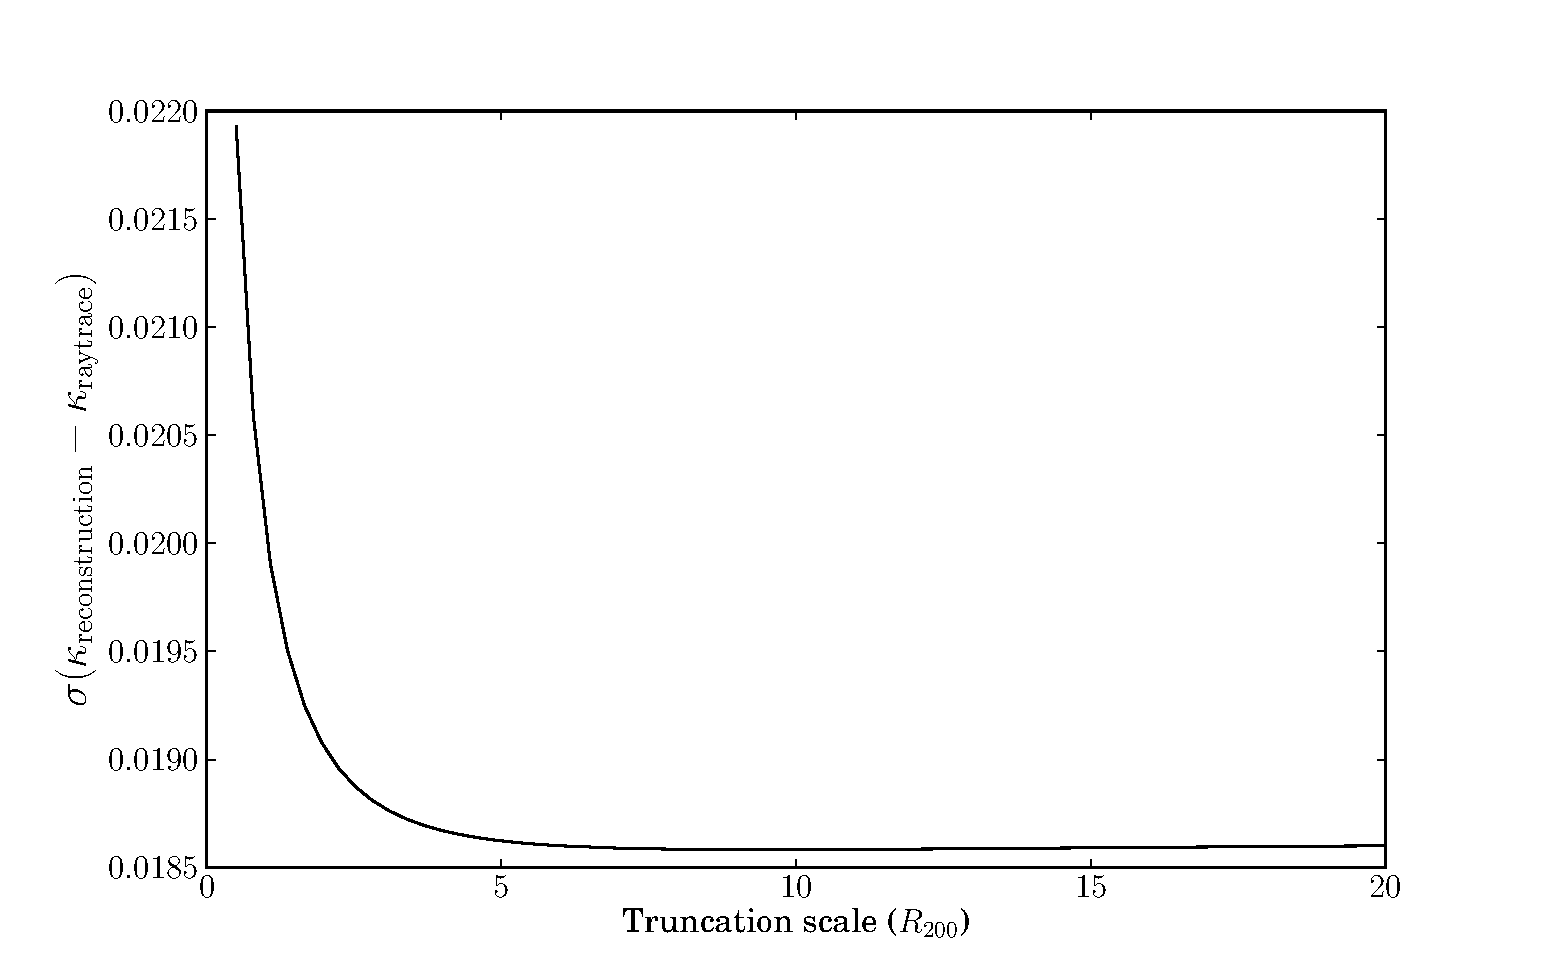
\includegraphics[width=\columnwidth]{figs/truncation_scatter.eps}
\caption[magcut]{The standard deviation in $\kapparec$ minus $\kapparay$ as a function of halo truncation radius in virial radii, using the truncated NFW profile of \citet{BMO}. In our models we truncate our halos at 5$R_{200}$}
\label{fig:ScattervsTruncation}
\end{figure}

For $\sumkappah$ to provide useful constraints on $\kapparay$, it is important that $\kapparay$ and $\sumkappah$ are as similar as possible. Figure \ref{fig:bias} shows that indeed $\sumkappah$ is a good estimator, regardless of the individual value of $\sumkappah$. At fixed $\sumkappah$ we find that the scatter in $\kapparay$ grows with $\sumkappah$; our reconstruction is better at reproducing underdense lines of sight than overdense lines of sight.

\begin{figure}
% 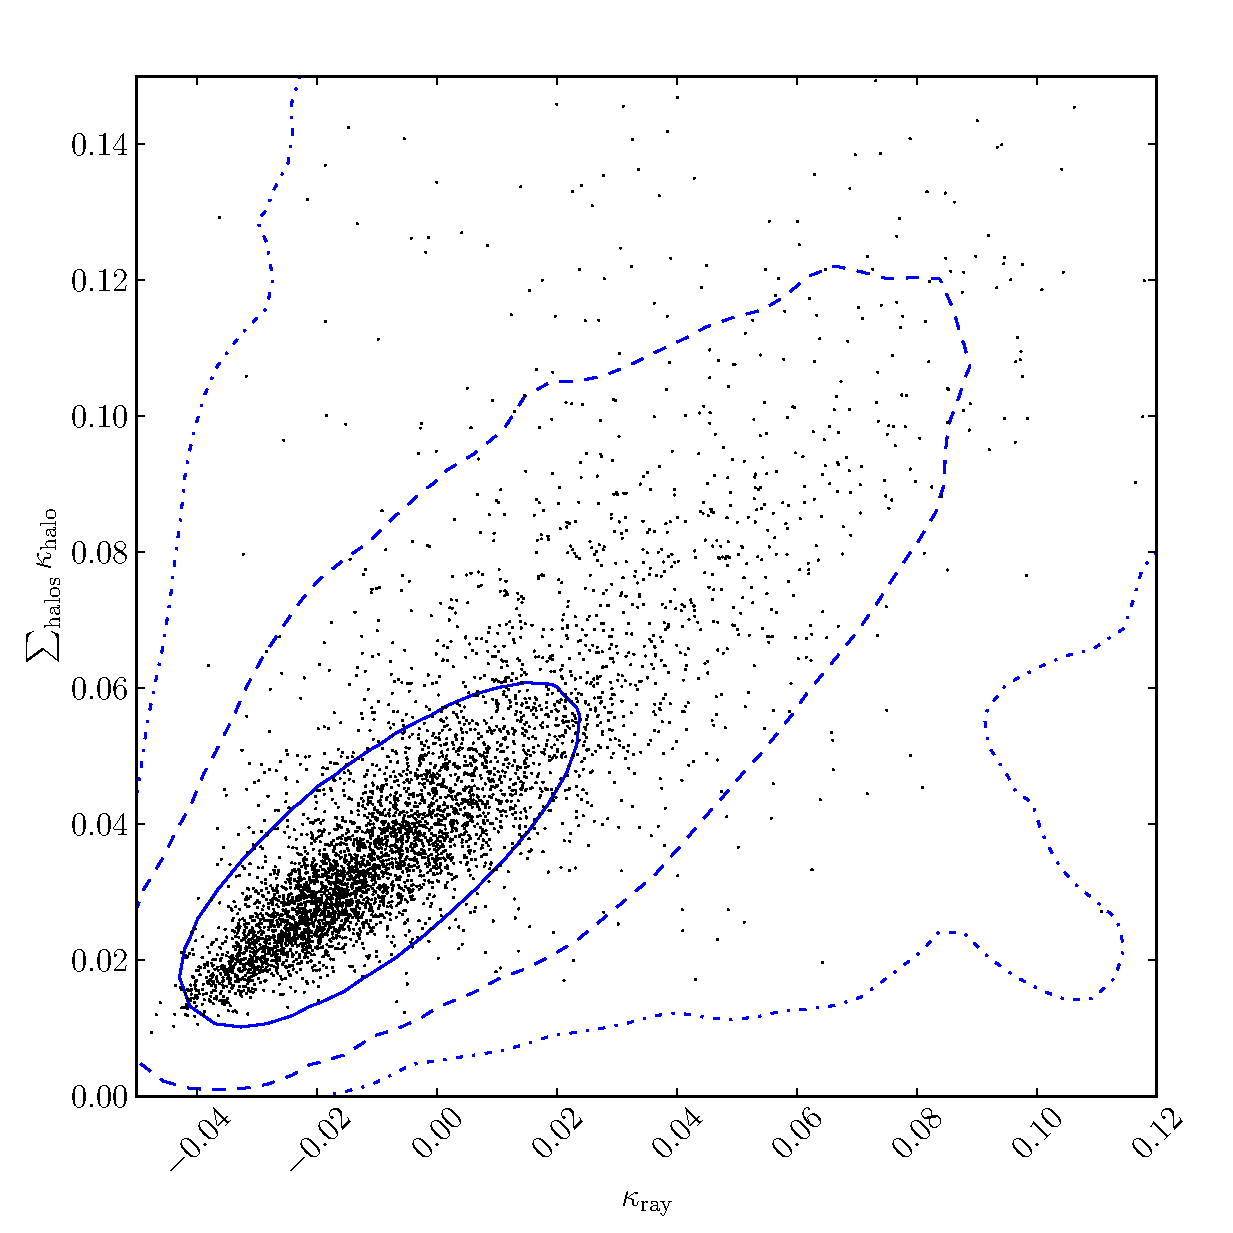
\includegraphics[width=\columnwidth]{figs/perfectc.eps}
\caption[Biased?]{$\sumkappah$ verses $\kapparay$ for 100000 reconstructed lines of sight. $\sumkappah$ traces $\kapparay$, but with a non-zero offset which is due to the negative connvergence from voids. At fixed $\sumkappah$ the scatter in $\kapparay$ grows with $\sumkappah$.}
\label{fig:isitbiased}
\end{figure}

The intrinsic error between the results of the halo based prescription and the raytraced convergence is an unavoidable error, even with perfect knowledge of halo mass and position. Before investigating the errors caused by imperfect knowledge of halo mass and redshift, we investigate the errors induced by a magnitude limited reconstruction and a field of view limited reconstruction. The halos in our catalogue are given magnitudes by the semi-analytic model of \citet{deLucia+Blaizot2007} and by applying magnitude cuts to our catalogue, we can investigate the scatter caused by unobserved halos. The majority of the convergence comes from halos with an $i$ magnitude between 18 and 24. Figure \ref{fig:magcut} shows that the width of $\kapparec-\kapparay$ decreases quickly between $i=18$ and $i=24$. Objects brighter than $i=18$ are either too rare or too close to the observer to make a significant contribution to the convergence. Objects fainter than $i=24$ are too small to be important, unless they are extremely close to the line of sight where it is likely that neglecting stellar mass and using a spherical NFW prescription are too naive to adequately reconstruct $\kappax$. It is likely that ultra-faint halos (or substructures), the uncertain contribution of voids and halos deviating from our spherical truncated NFW profile are the three major sources of the scatter in $\kapparec-\kapparay$; a deeper survey will not be sufficient to decrease the size of this scatter. Since a large number of callibration lines of sight must be reconstructed to sample $\pr(\kappav)$, it may prove unrealistic to reconstruct the calibration lines of sight out to 5 arcminutes. Figure \ref{fig:radcut} shows the width of $\kapparec-\kapparay$ as a function of reconstruction radius; in almost all cases there is no significant contribution to $\kappa$ from halos that are centred more than 1 arcminute away, although large groups or clusters can sometimes still make a contribution as far out as four arcminutes. For the rest of this work we will continue to model all of the halos out to 5 arminutes with an $i$ magnitude greater than 26, although a reconstruction with fields going out to two arcminutes and down to $i=24$ would do almost as well.

\begin{figure}
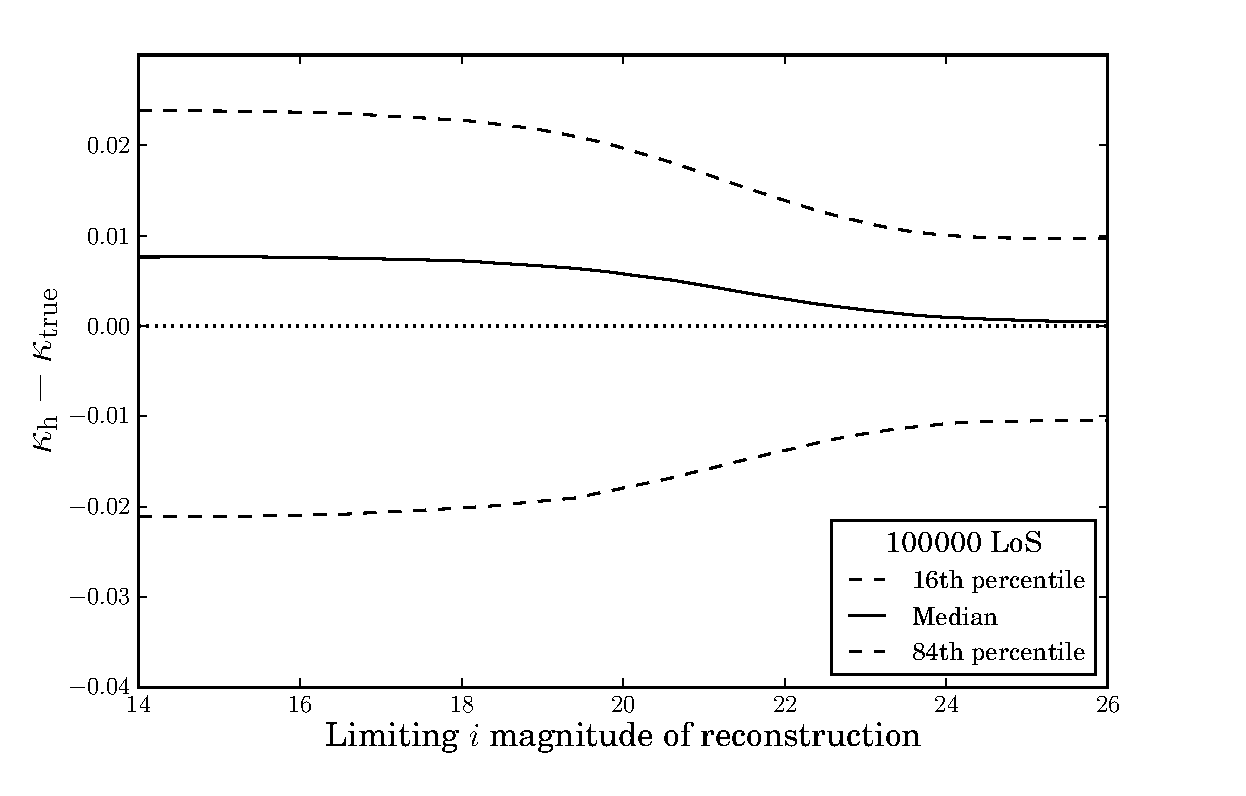
\includegraphics[width=\columnwidth]{figs/mag_scatter.eps}
\caption[magcut]{The 16, 50 and 84\% confidence intervals on $\kapparec$ minus $\kapparay$ as a function of the limiting $i$ band depth of the halo reconstruction. $\kapparec$ is given by $\sumkappah-\kappav$, where $\kappav$ is a constant such that $\left\langle\kapparec\right\rangle=0$. The majority of the constraining power comes from reconstructing halos with magnitudes between $18<i<24$}
\label{fig:magcut}
\end{figure}
\begin{figure}
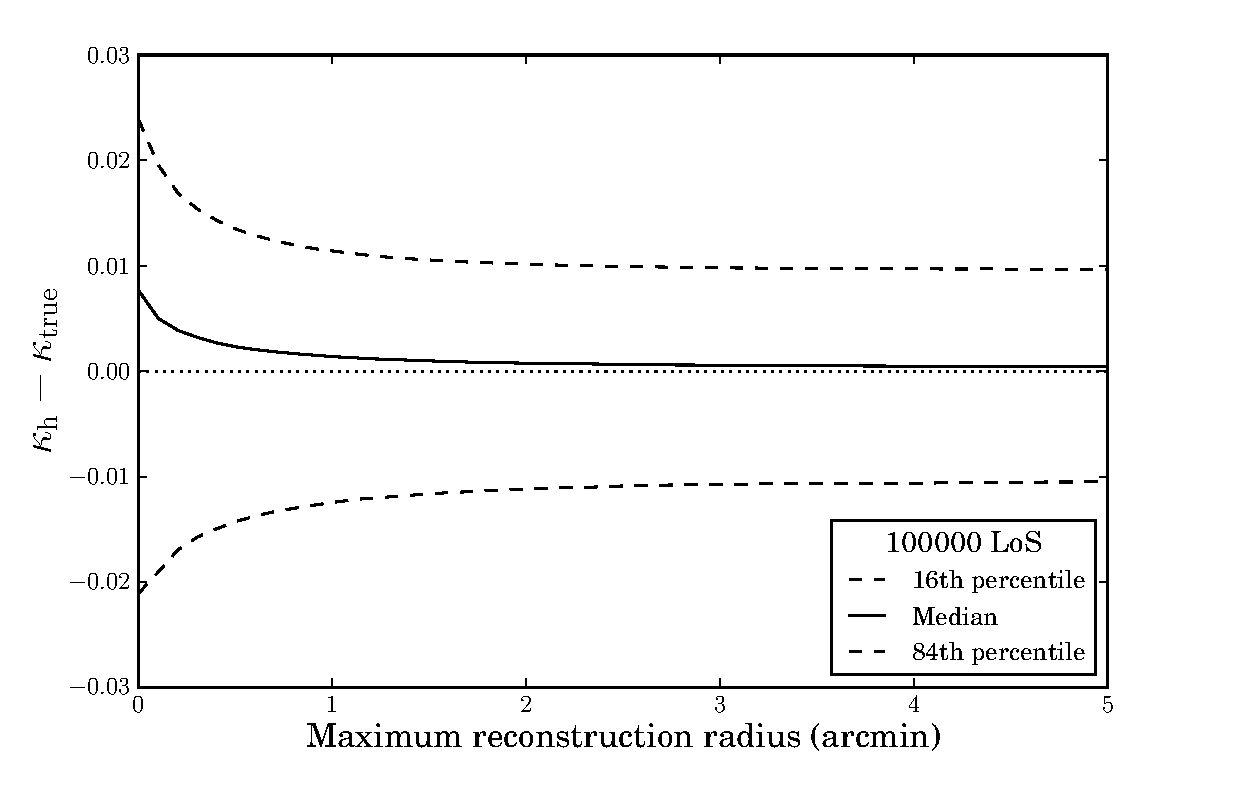
\includegraphics[width=\columnwidth]{figs/radius_scatter.eps}
\caption[radius cut]{The 16, 50 and 84\% confidence intervals on $\kapparec$ minus $\kapparay$ as a function of the limiting radius (in arcminutes) beyond which halos are not reconstructed. The majority of the convergence comes from halos centred within an arcminute of the line of sight}
\label{fig:radcut}
\end{figure}

The final test that we apply to the perfect knowledge reconstruction is to apply the marginalization outlined in Section \ref{subsec:voids}. Taking the reconstructed $\sumkappah$ for $1\times 10^{5}$ lines of sight we form the joint distribution, P$(\kapparay,\sumkappah)$ and marginalize over all sightlines with a similar $\sumkappah$ to give P($\kappax$). We define the bias as the difference between the expectation value of $\kappax$ and the known true value of $\kapparay$ for each Line of sight and we define the reconstruction width as half the width of the interval containing the central $68\%$ of the probability P($\kappax$). From $1\times 10^{4}$ reconstructed lines of sight we find the the bias to have mean of $-9.5\times 10^{-6}$ and a mean reconstruction width of 0.0132. In the case where one assumes P$(\kappax)$ is given by the global P$^{\rm global}(\kappax)$, the same $1\times 10^{5}$ lines of sight show a mean bias of $4.3\times 10^{-5}$ and mean reconstruction width of 0.237. Within the statistical error both methods are unbiased, but for any individual line of sight the bias is typically 1.8 times smaller with the reconstructed P$^{\rm reconstruction}(\kappax)$, rather than global P$^{\rm global}(\kappax)$. 

%%%%%%%%%%%%%%%%%%%%%%%%%%%%%%%%%%%%%%%%%%%%%%%%%%%%%%%%%%%%%%%%%%%%%%%%%%%%%%%%

\section{Applying the Halo Model approximation to mock catalogs}
\label{sec:obsMstar+z}

Real attempts to reconstruct the convergence along a line of sight will not have direct access to the masses of dark matter halos, 
and will likely not have access to their spectroscopic redshift either. Instead these properties must be inferred from astrophysical
observables. In principle the only observables are astrometric positions, photometric colours and possibly spectra. In this section we
quantify the errors induced by inferring the halo mass and redshift from the observables. Much work has already focused on using
photometric colours to infer stellar mass \citep[\eg][]{xxx} and redshifts \citep[\eg][]{BPZ}, in line with these we shall use
stellar mass and photometric redshifts (with appropriate errors), as the observables that must be converted into an estimate
of $\kappax$. We will investigate two main sources of error: inferring halo mass given observed stellar mass and placing halos at the wrong redshift due to photometric redshift error.

We generate a stellar mass for each halo according to the stellar mass--halo mass relation of \citet{BehrooziEtal2010}. From this stellar mass we simulate 
an observed stellar mass by drawing a sample from $\pr(\log(M_{* \mathrm {obs}})|\log(M_{* \mathrm {true}}))$ which is given by \comments{ the product of the galaxy stellar mass function (GSMF) of \citet{Fontana2006} and} a Gaussian of width $\sigma_{M_*}$ centred on $\log(M*_{\mathrm {true}})$. Where a spectroscopic redshift exists stellar masses can be estimated with typical uncertainties of 0.15 dex \citep{xxx}, however with photometric redshifts stellar mass uncertainties are typically three times as large \citep{xxx}; we use $\sigma_{M_*}=0.15$ for halos with a spectroscopic redshift and $\sigma_{M_*}=0.45$ otherwise. \comments{The \citet{Fontana2006} GSMF is given by a Schechter function with redshift evolving parameters
\be
\label{eq:GSMF}
{\dee N \over \dee M_*} \propto \left(10^{(M_*-M_0(z))}\right)^{(1+\alpha(z))} \exp \left(-10^{(M_*-M_0(z))}\right)
\ee 
where $M_0(z)=11.16+0.17z-0.07z^2$ and $\alpha(z)=-1.18-0.082z$.} For photometric redshift errors we draw a redshift from $\pr(z_{\rm true}|z_{\rm obs})$ which we take as a Gaussian of width $0.1(1+z_{\rm spec})$ centred on $z_{\rm spec}$, where $z_{\rm spec}$ is the halo's true redshift in the \MS catalogue

For each  source of error, we reconstruct 40000 calibration lines of sight and 10000 mock lens lines of sight, following the proceedure outlined in Section \ref{sec:model}. Reconstructing the lines of sight with perfect knowledge of the redshift but an uncertain stellar mass, we find that the width of $\Pr\left(\sumkappah \right)$ grows with the expectation value of $\sumkappah$; this is not surprising since the low $\sumkappah$ lines of sight are relatively empty and so there are few opportunities for uncertainties in the halo masses to propogate into $\sumkappah$ uncertainties. After applying the void correction the expected bias from our 10000 mock lenses is $6.7\times 10^{-5}$ and the mean reconstruction width is 0.0145; this is the typical reconstruction error that could be expected from a complete spectroscopic survey of the field, it is ten percent worse than the reconstruction given perfect knowledge of the halo masses and redshifts but still 1.6 times better than using the global P$^{\rm global}(\kappax)$ although a complete spetroscopic survey is still unrealistic. The distribution of the widths of $\Pr\left(\kappax \right)$ is shown in Figure \ref{fig:width1}


\begin{figure}
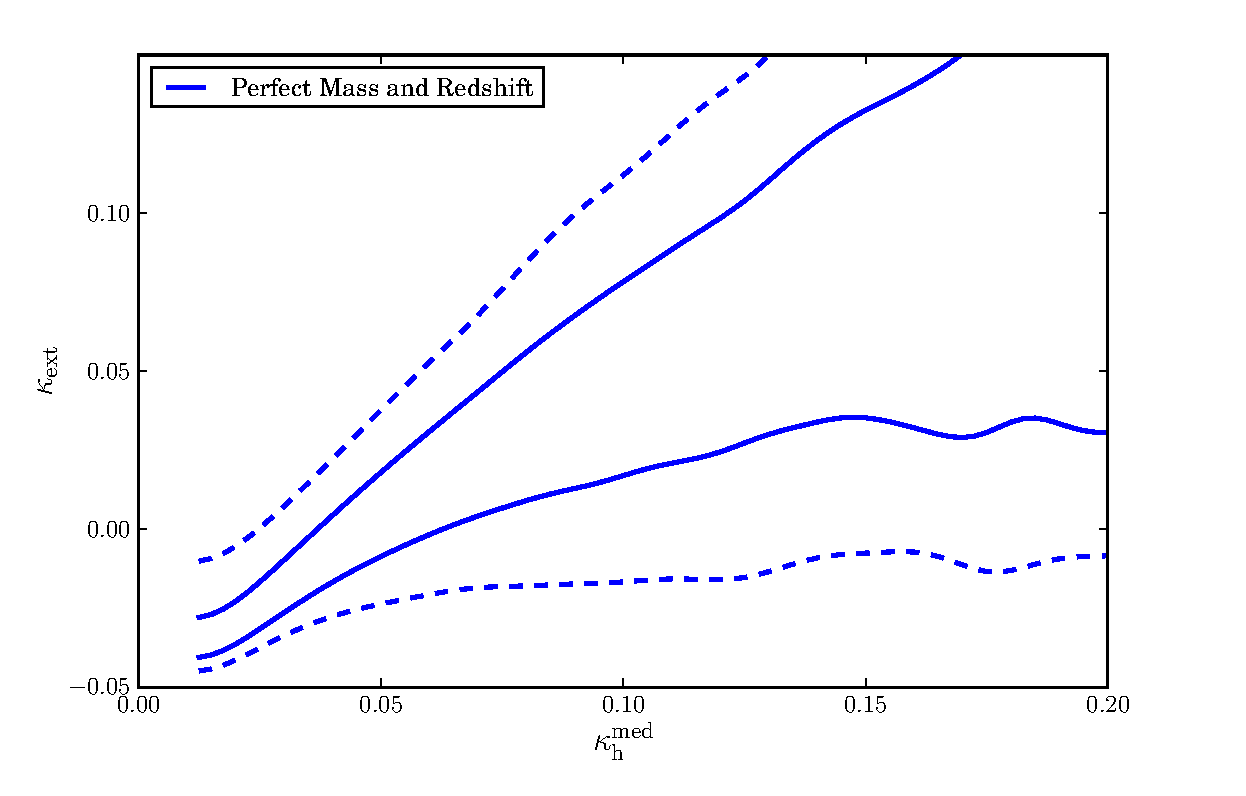
\includegraphics[width=\columnwidth]{figs/cornerplot.eps}
\caption{68 \% and 95 \% contours of the joint distribution $\pr(\kapparay, \tilde\kappa_{\rm halos})$ given a mock reconstruction of our 40000 calibration lines of sight. $\tilde\kappa_{\rm halos}$ is the median of $\pr(\sumkappah)$ given a spectroscopic redshift for each halo. $\kapparay$ and $\tilde\kappa_{\rm halos}$ are strongly correlated, despite the blurring effect of uncertain halo masses.}
\label{fig:corner}
\end{figure}

\begin{figure}
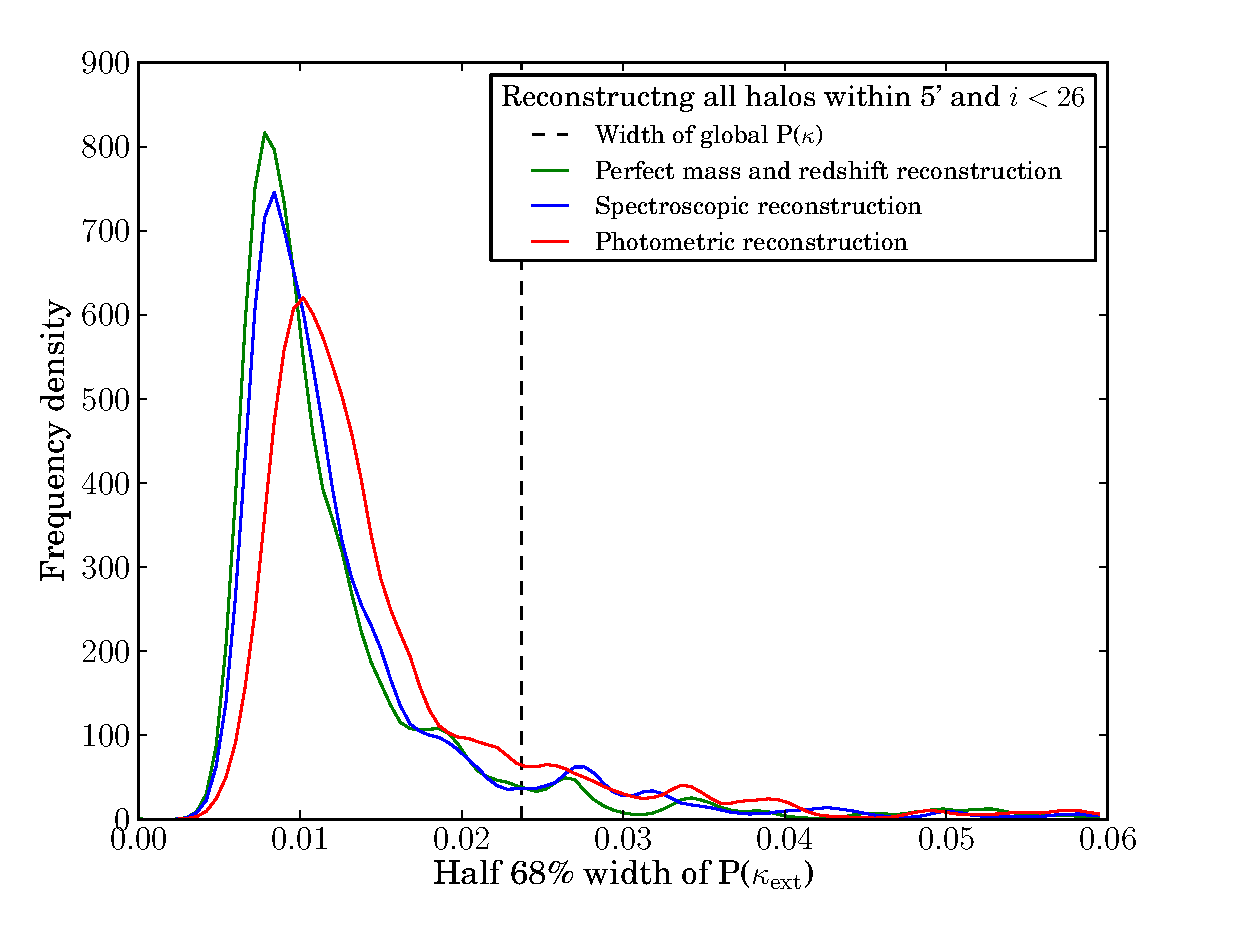
\includegraphics[width=\columnwidth]{figs/widths.eps}
\caption{Widths of $\pr(\kappax)$ after applying our reconstruction of all halos down $to i=26$ and within 5 arcminutes of the line of sight. Results for 10000 lines of sight are shown. Green is for a reconstruction given perfect knowledge of halo mass and redshift, blue is for a reconstruction given a spectroscopic redshift for every halo, and red is for a reconstruction with photometric redshifts only. The dashed black line shows the width of the global $\pr(\kappax)$ distribution; the reconstruction process provides roughly a factor of 2 improvement for the majority of lines of sight. Spectroscopic redshifts improve the reconstruction, but at signifcant observational cost.}
\label{fig:width1}
\end{figure}

Inferring the stellar mass of a galaxy from its magnitude and colours requires an estimate of how far away the galaxy is; without a spectroscopic redshift the the infered stellar mass is less precise. In principle the photometric redshift is correlated with the infered stellar mass, however we do not model this effect since the convergence from the outskirts of an individual halo is only weakly dependant on redshift at fixed mass: the redshift error is small effect on the recovered $\pr(\kappa)$ when compared to the effect of uncertain stellar masses.  With only photometric redshifts the uncertainty on $\sum\kapparec^{\rm halos}$ is much larger than the spectrocopic case, but this does not propogate into a much larger bias after applying the void correction; with a purely photometric reconstruction of the 10000 mock lightcones the results have a mean bias of $1.1\times 10^{-4}$ and a mean width of 0.0158. On average a purely photometric reconstruction of the field gives an unbiased $\pr(\kappax)$ that is 1.5 times tighter than assuming the global $\pr^{\rm global}(\kappax)$. 


%\subsection{Reconstructions of Smaller and Shallower Fields}

\begin{figure}
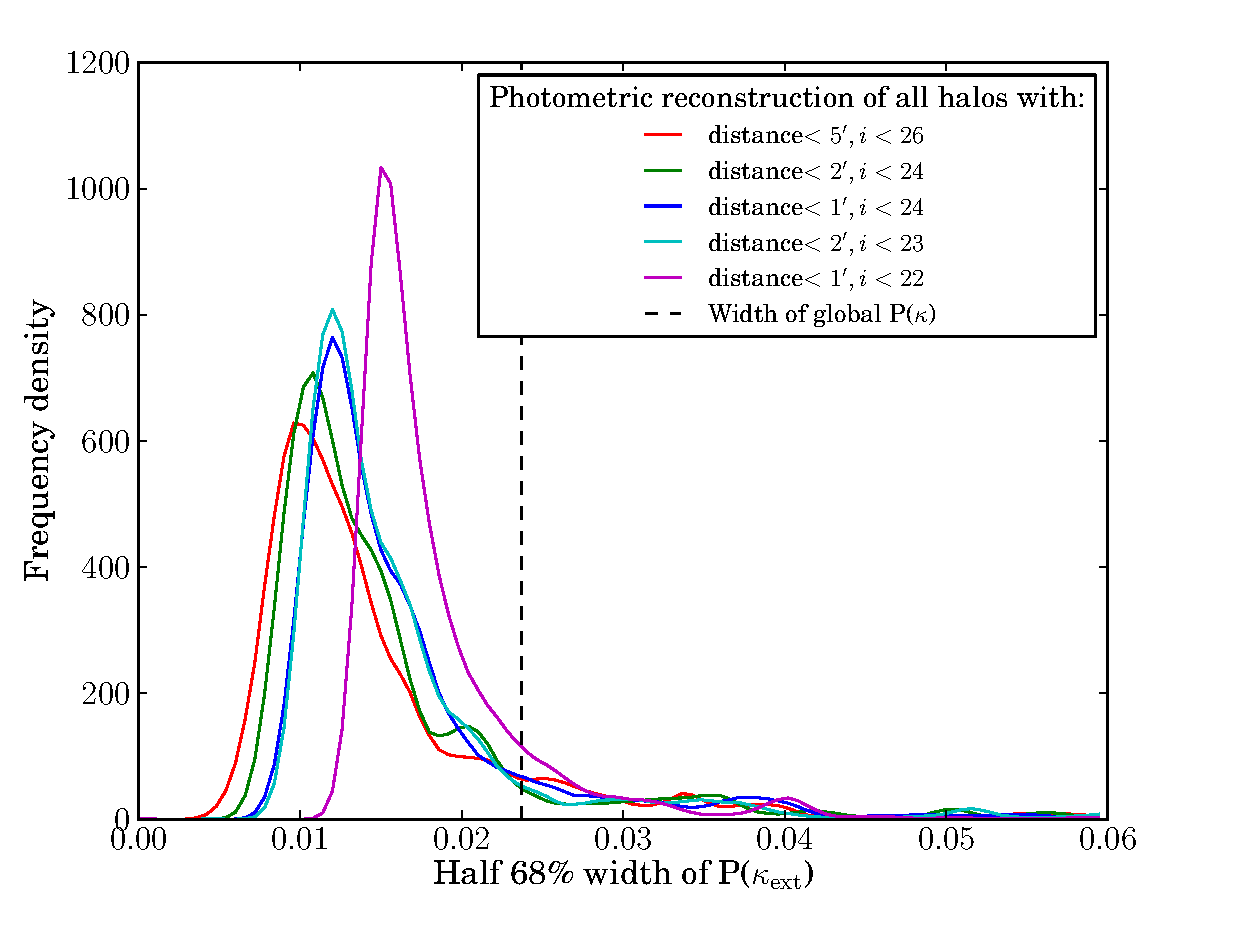
\includegraphics[width=\columnwidth]{figs/widths2.eps}
\caption{Widths of $\pr(\kappax)$ after a photometric reconstruction of all halos within different fields. The different field sizes and depths are given in the legend. As the field becomes smaller or shallower, fewer halos are being reconstructed and so the width of $\pr(\kappax)$ grows.}
\label{fig:width2}
\end{figure}


Reconstructions of real lines of sight may not have access to the deep, large calibration fields that we have used upto this point. We can perform the same reconstruction but for a more modest mock survey. Given the results of Section \ref{sec:knownMh+z} we predicted that a reconstruction of the field out to 2 arcminutes and a magnitude limit of $i$=24 would provide similar constraints to a reconstruction going out to 5 arcminutes and going down to $i$=26. We find the mean reconstruction width to be 0.0163 for a photometric reconstruction of all the halos within 2 arcminutes that have $i<24$, this is only marginally worse than 0.0158 which was the typical width after the deeper and wider reconstruction of the previous section. The reconstruction widths for our 10000 mock lens lines of sight are shown in Figure \ref{fig:widths2}. If only photometry for halos with $i<24$ and within 1 arcminute of the line of sight is availble then the typical width of the reconstructed $\pr(\kappax)$ is 0.173. Whilst a complete spectroscopic survey of a large field would be unlikely, a hybrid strategy of obtaining spectra for a subset of objects may be feasible. Photometric redshifts are sufficient to asertain the halos which are likely to contribute most of the convergence on any given line of sight, and on average there are only $\sim 6 \pm 6$ halos per line of sight that individually contribute more than 0.002 to $\sumkappah$. We investigate a hybrid strategy of obtaining spectroscopic redshifts for all of the $i<24$ halos which contribute an individual $\kappa$ of at least 0.002 combined with a photometric redshift for all other $i<24$ halos within 2 arcminutes. For the hybrid strategy the typical width of the reconstructed $\pr(\kappax)$ is 0.0151. The observational cost of obtaining spectroscopic redshifts for several 24th magnitude galaxies may make the hybrid strategy unlikley, but obtaining photometry of a 4$\times$4 arcminute patch of sky down to $i=24$ is fast with modern telescopes. The mean reconstruction width for a photometric reconstruction of all the halos within 2 arcminutes that have $i<24$ represents an improvement of 1.5 over using the global $\pr(\kappax)$ and should be achievable at minimal observational cost.


%%%%%%%%%%%%%%%%%%%%%%%%%%%%%%%%%%%%%%%%%%%%%%%%%%%%%%%%%%%%%%%%%%%%%%%%%%%%%%


\section{Testing for Systematic errors}
\subsection{Using the wrong M$_{\rm halo}$-M$_{*}$ relation}
\subsection{Selecting bias from a subset of lines of sight?}
\subsubsection{Selecting only the lines of sight with tight $\pr(\kappax)$}
\subsubsection{Selecting only high shear lines of sight}

%%%%%%%%%%%%%%%%%%%%%%%%%%%%%%%%%%%%%%%%%%%%%%%%%%%%%%%%%%%%%%%%%%%%%%%%%%%%%%
\comments{

\subsection{Comparison with Other Treatments of $\kappax$}
\label{sec:Dt:selection} 

\phil{How does distance accuracy compare with simple averaging? eg assuming
$\kappax = 0$ for all lenses. How does it compare with the no data situation?
eg where the intrinsic distribution of kappa is used as $Pr(\kappax)$.}

What is the expected bias and scatter (centroid position and width) of P(D) as a
function of N lenses? How does reconstruction compare with P(D) derived using
P(kappa|N45) for each lightcone? How does reconstruction compare with P(D)
derived assuming kappa=0 for each lightcone?

Also: compare with simple averaging. This will fail if lenses are selected to
live on over-dense lines of sight. Stefan's plot in Suyu et al shows effect of
selection - what is the resulting bias? Few percent? This is the target to beat,
need to find it out.

\subsection{Improving the Accuracy with More Information}
\label{sec:Dt:selection} 

\phil{How does distance accuracy improve with:}
\begin{itemize}
\item Spectroscopic coverage? For galaxies above some mlim? For targets with
high kappa contribution (based on photometry)?
\item IR coverage for all objects? Improves photo-z and Mstar.
\item Including shear information from lens model? Assume accurate but
uncertain extertanl shear.
\end{itemize}
}
%%%%%%%%%%%%%%%%%%%%%%%%%%%%%%%%%%%%%%%%%%%%%%%%%%%%%%%%%%%%%%%%%%%%%%%%%%%%%%

\section{Discussion}
\label{sec:discuss}

We have shown that reconstructing the matter due to halos along any line of sight can give meaningful and unbiased constraints on the external convergence along that line of sight. The total convergence along a line of sight is strongly correlated with the reconstructed $\sumkappah$. However since our model ignores voids and assumes all halos follow a spherical truncated-NFW profile our model does not include all of the relevant physics, hence the width of our resulting $\pr(\kappax)$ is still typically $\sim$0.01, even with a perfect knowledge of every halo's virial mass and redshift. To make further progress a more advanced treatment of both voids and halos will be necessary. Interestingly, we have found that the most empty lines of sight can be reconstructed with the most precision. $\kappax$ for empty lines of sight have little contributions from halos and a large contribution from voids; since they have the tightest PDFs after the reconstruction it seems that our model's biggest uncertainties are driven by naively reconstructing halos rather than neglecting voids. With a photometric reconstruction of the field there is only a small broadening compared to the perfect knowledge reconstruction; it seems that deviations from sphericity and dark matter clumping within the main halo are the dominant uncertainies rather than uncertainties in the halo mass. Inferring halo ellipticity and dark matter clumping will likely always remain a difficulty for line of sight reconstruction; as Figures \ref{fig:magcut} and \ref{fig:width2} show observing deeper than 24th magnitude does not signifcantly help the reconstruction. Because our reconstruction is mostly limited by the model, spectroscopic coverage can only provide a modest improvement to the reconstruction and at significant observational cost.

For a small fraction of lines of sight, $\pr(\kappax)$ remains very broad even after applying our reconstruction; these lines of sight are typically the most overdense lines of sight in the universe. For time-delay cosmography the most observationally expensive task is the lightcurve monitoring, whilst making photometric observations of a 4$\times$4 arcminute patch of sky survey down to 24th magnitude is a relatively cheap. We have shown that with a single epoch observation of the region around a strong lens it is possible to infer $\pr(\kappax)$. If a line of sight has a broad $\pr(\kappax)$ it can be rejected {\it before} the investment of longterm lightcurve monitoring.

The method we have outlined can also be used to estimate the external shear
along a line of sight. Shear is an observable that can be extracted from
strong lens modelling, however there is a degeneracy between internal and
external shear. Progress has been made in disentangelling external and
internal shear \citep[\eg][]{xxx} but there are still significant
uncertainties: \citet{WongEtal2011} attempted to match the shear from strong
lens models with a reconstruction of the local lens group environment, but
found a tension between the strong lens model and the reconstruction of the
environment. Since \citet{WongEtal2011} only reconstructed the local lens
group, rather than the full line of sight contribution, it is unclear whether
the external shear from lens models can be reconciled with a line of sight
reconstruction. {\it If} external shear can be measured, it provides an
additional constraint on which of the Millenium Simulation lines of sight are
similar to the reconstructed line of sight. \citet{SuyuEtal2012} found that
for RXJ1131 combining shear constriants with galaxy number count overdensity,
gave a significantly different $\pr(\kappax|\gamma,N_{45})$ copmpared to the
PDFfrom number count overdensity alone, $\pr(\kappax|N_{45})$. 



%%%%%%%%%%%%%%%%%%%%%%%%%%%%%%%%%%%%%%%%%%%%%%%%%%%%%%%%%%%%%%%%%%%%%%%%%%%%%%

\section{Conclusions}
\label{sec:conclude}

In this work we have investigated a simple halo model prescription for
reconstructing all the mass along a line of sight to an intermediate redshift
source. We have used the ray-traced lensing convergence along lines of sight
through the Millenium Simulation to test this approach, and to calibrate
estimates of the total convergence along a line of sight to an observed
distant galaxy made by summing the convergences due to each object in a
photometric catalogue. Having found that the reconstruction process is effective given perfect
knowledge of halo mass and redshift, we investigated the effects of reasonable
uncertainties in the stellar mass and redshift of each halo, and propogated
these uncertainties into a $\pr\left(\sumkappah\right)$ for each line of
sight. We draw the following conclusions:

\begin{itemize} 

\item Our model uses a truncated spherical NFW profile for
each dark matter halo and neglects voids, but despite the model's simplicity
the reconstructed $\sumkappah$ is a good tracer of $\kappax$.  We found that
with perfect knowledge of the halo mass and redshift (from the Millenium
Simulation catalogs), the reconstruction gives an unbiased estimate of
$\pr(\kappax)$ for a single line of sight that is almost almost a factor of 2
less broad than the global $\pr(\kappax)$. 

\item  For the most overdense lines of sight, the reconstruction produces a
very broad PDF, but since the reconstruction can be performed before follow-up
time is invested it will be possible to discard the most uncertain lines of
sight and prevent the waste of follow-up time. 

\item With complete spectroscopic redshift coverage and just an empirical
stellar mass to halo mass relation, we find that the median of
$\pr\left(\sumkappah\right)$ is a useful indicator for generating an estimate
of $\pr(\kappax)$ from the ensemble of simulated lines of sight. The resulting
PDF tends to be around 10\% broader than it would have been given perfect
knowledge of both halo mass and redshift; given only photometric redshifts
(which in turn give rise to much less certain stellar masss estimates) causes
another $\sim$10\% increase to the width of $\pr(\kappax)$.

\item It is very rare for halos further than 2 arcminutes to make a
significant contribution to $\kappax$. We also found that including halos
whose host galaxy is less luminous than $i=24$ does not significantly improve
our reconstruction proceedure. A photometric survey to this depth of a
4$\times$4 arcminute patch around the lens would approach the limiting
uncertainties of our simple reconstruction recipe, and yield a 
$\pr(\kappax)$ that has, on average, a width of 0.0163 --
50\% less broad than the global $\pr(\kappax)$.

\item We find that the lines of sight with the sharpest $\pr(\kappax)$ are
typically under-dense. With a photometric reconstruction of all lens fields,
and following up only the lenses with the most constraining $\pr(\kappax)$,
the width of the dominant statistical uncertainty in time-delay cosmography
can be halved, whilst at the same time decreasing any potentail for a
systematic error due to lenses being biased in $\kappax$.

\end{itemize}

\todo{Tom}{Add more conclusions about bias in a large sample of lenses...}

\todo{Tom}{Wrap up}


%Our conclusions can be summarised as follows:
%\begin{itemize}
%\item With perfect 
%\item And we found this too.
%\end{itemize}

% \item Faint galaxies and other dark structures will not appear in a photometric
% object catalog, but they will contribute convergence at some level. How much of
% the total external convergence in a time delay lens system comes from visible
% galaxies? How does this change as a function of magnitude cut? 

% \item Can the true (ray-traced) convergence be recovered by halo model
% reconstruction, and with what scatter and residual bias? Which aspects of the 
% model dominate these uncertainties?

% \item When faced with a newly-detected lens, surrounded by galaxies on the sky,
% we have some choices to make when planning follow-up observations.
% Which are the most important galaxies, with regard to the external convergence
% produced? Can nearby groups and clusters be straightforwardly accounted for? If
% lenses with such massive structures nearby are discarded, what impact does that
% have on the distance accuracy?



%%%%%%%%%%%%%%%%%%%%%%%%%%%%%%%%%%%%%%%%%%%%%%%%%%%%%%%%%%%%%%%%%%%%%%%%
%%  ACKNOWLEDGMENTS
%%%%%%%%%%%%%%%%%%%%%%%%%%%%%%%%%%%%%%%%%%%%%%%%%%%%%%%%%%%%%%%%%%%%%%%%

\section*{Acknowledgments}
 
TC thanks Vasily Belokurov for guidance and discussions.
We thank Risa Wechsler and Peter Behroozi for useful discussions and 
suggestions.
TEC acknowledges support from STFC in the form of a research studentship.
%
PJM was given support by the Kavli Foundation and the Royal 
Society, in the form of research fellowships.
%
MWA \ldots
%
SH \ldots
%
SHS \ldots
%
TT acknowledges support from the NSF through CAREER award NSF-0642621,
and from the Packard Foundation through a Packard Research Fellowship.
% 
LVEK acknowledges the support by an NWO-VIDI programme subsidy
(programme number 639.042.505).
%
This research is supported in part by the National Science Foundation under
Grant No. PHY99-07949.



%%%%%%%%%%%%%%%%%%%%%%%%%%%%%%%%%%%%%%%%%%%%%%%%%%%%%%%%%%%%%%%%%%%%%%%%%%%%%%
%  APPENDICES
%%%%%%%%%%%%%%%%%%%%%%%%%%%%%%%%%%%%%%%%%%%%%%%%%%%%%%%%%%%%%%%%%%%%%%%%%%%%%%

\appendix

%%%%%%%%%%%%%%%%%%%%%%%%%%%%%%%%%%%%%%%%%%%%%%%%%%%%%%%%%%%%%%%%%%%%%%%%%%%%%%

\section{Truncated NFW halos}
\label{appendix:halos}

 Defining $x$ as the dimensionless projected radial distance $R/r_{s}$ and $\tau$ as the dimensionless truncation radius $r_{t}/r_{s}$, \citet{BMO} derives the projected mass density, which is given by:
\begin{align}\label{eq:kappaBMO}
\Sigma_{\rm}(x) = {2\tau^2 \over (\tau^2+1)^2}\left(
        {\tau^2+1\over x^2-1}\left(1-\mathcal{F}(x)\right)
        +
        2\mathcal{F}(x)\right.\nonumber\\
        -
        \left. {\pi \over \sqrt{\tau^2+x^2}}
        +
        {(\tau^2-1)\mathcal{L}(x,\tau)
        \over
        \tau\sqrt{\tau^2+x^2}}\right)
\end{align}
where $\mathcal{F}(x)$ and $\mathcal{L}(x,\tau)$ are defined as
\be\label{eq:F} 
\mathcal{F}(x) \equiv \begin{cases}  \frac{{\rm cos}^{-1} (1/x)}{\sqrt{x^2-1}} \hspace{0.2cm} & (x>1) \\
\\
\frac{4-x^2}{3}  & (x=1)\\
\\
\frac{ {\rm cosh}^{-1} (1/x)}{\sqrt{1-x^2}} & (x<1)
\end{cases}
\ee
\be\label{eq:L}
\mathcal{L}(x,\tau) = \ln\left(\frac{x}{\sqrt{\tau^2+x^2}+\tau}\right)
\ee
%the convergence is given by $\Sigma_{\rm BMO}(x) / \Sigma_{\rm cr}(z)$.



%%%%%%%%%%%%%%%%%%%%%%%%%%%%%%%%%%%%%%%%%%%%%%%%%%%%%%%%%%%%%%%%%%%%%%%%%%%%%%

\section{Inferring $\Mhalo$ given a noisy measurement of $\Mstarobs$}
\label{appendix:MSMH}

Given a noisy estimate of the stellar mass $\Mstarobs$ of a galaxy at redshift
$z$, how can we infer the galaxy's halo mass? We then seek the posterior
PDF $\Pr(\Mhalo|\Mstarobs)$, which can be expanded as follows:

\begin{eqnarray}
&& \Pr(\Mhalo|\Mstarobs,z) = \notag\\
&& \int d\Mstar \Pr(\Mhalo|\Mstar,z) \Pr(\Mstar|\Mstarobs,z), \notag\\
&\propto& \int d\Mstar \Pr(\Mstarobs|\Mstar) \Pr(\Mstar|\Mhalo,z) \Pr(\Mhalo|z),
\label{eq:mhalo-mstar}
\end{eqnarray}
where we have used Bayes' Theorem twice to replace
$\Pr(\Mhalo|\Mstar,z) \Pr(\Mstar|z)$ with 
$\Pr(\Mstar|\Mhalo,z) \Pr(\Mhalo|z)$, and 
to invert $\Pr(\Mstar|\Mstarobs)$ into the sampling
distribution $\Pr(\Mstar|\Mstarobs)$, which we recognise as the likelihood
function for the observed stellar mass. Note that the ``true'' $\Mstar$ of the
galaxy is marginalised out: we are only interested in reconstructing the halo
mass. The last two terms in
\eqref{eq:mhalo-mstar} are the $\Mstar-\Mhalo$ relation from
\citet{BehrooziEtal2010}, and the halo mass function $\Pr(\Mhalo|z)$, at the
given redshift. We can
tabulate the product of these two from our Millenium Simulation catalog,
constructing a two-dimensional histogram of halo masses and their associated
true stellar masses (drawn from the Behroozi relation). 

For each galaxy, we compute the likelihood function for its $\Mstarobs$ as a
function of the unknown $\Mstar$, and multiply it by our tabulated joint PDF.
This heavily downweights halos with $\Mstar$ values outside the observed
range. We then do the marginalisation integral by Monte Carlo, drawing
(two-dimensional) sample parameter vectors
from the downweighted histogram, discarding the $\Mstar$ values, and
constructing a one-dimensional histogram that is an estimate of
$\Pr(\Mhalo|\Mstarobs)$.

\todo{Matt}{Edit the above text to add a note on how we do the sampling in
practice, via the CDF.}

If the redshift of the galaxy is uncertain, we need to take this uncertainty
into account; for example, for each sample drawn from the photometric redshift
posterior PDF $\Pr(z|{\rm colors})$, we can draw a sample $\Mhalo$ using the
above procedure.


%%%%%%%%%%%%%%%%%%%%%%%%%%%%%%%%%%%%%%%%%%%%%%%%%%%%%%%%%%%%%%%%%%%%%%%%%%%%%%

\section{Accounting for uncatalogued low mass halos, and voids}
\label{appendix:smooth}

Our halo model allows us to infer a halo mass $\Mhalo$ for each galaxy in a
photometric catalog; under the weak lensing approximation described in
\Sref{sec:theory} we can compute the contribution of each of these halos to
the overall convergence and shear amplitude, assuming a homogeneous
Friedman-Robertson-Walker metric and the concordance $\Lambda$CDM cosmological
parameters for the angular diameter distances to calculate the critical
density for each lens plane. Clearly this approach will tend to over-estimate
the convergence, since we are placing massive halos into a volume that has
already been assumed to be full of homogeneously distributed matter with the 
mean cosmological density. In practice, the space between massive halos will
contain a) low mass halos that are not bright enough to be detected and b)
empty space where the density is below that of the mean. A rigorous treatment
of this complex situation is beyond the scope of this paper, but is being
investigated (Blandford et al, in preparation). In this appendix we describe
our empirical approach to accounting for the missing mass and voids. 

Let the summed convergence due to halos in our galaxy catalog be $\kappah$.
Given some assumptions about halo density profile and shape, this parameter
can be inferred from a set of uncertain halo mass estimates (which have in
turn been inferred from noisy measurements of galaxy redshift and stellar mass
as described in \Aref{appendix:MSMH}). We assume each halo to be a
spherically-symmetric NFW profile, and neglect the contribution of the stellar
mass to the convergence. The halo mass inference for the $k^{\rm th}$ galaxy 
is stored as a list of sample values of $\Mhalok$ drawn from the posterior PDF
$\Pr(\Mhalok|\Mstarobsk,z_k)$; computing the contribution to the convergence
due to this halo at the target line of sight for each sample gives, in turn, 
a set of
samples drawn from the PDF $\Pr(\kappahk|\Mstarobsk,z_k)$. We then generate
samples from $\Pr(\kappah|\{\Mstarobsk,z_k\})$ by drawing a sample $\kappahk$
for each halo, summing over halos to get $\kappah$, discarding those
samples and moving down the lists.

The PDF $\Pr(\kappah|\{\Mstarobsk,z_k\})$ will, in general, be broad (due to
the uncertainties involved in halo mass estimation). It will also be shifted
towards high values of convergence, due to the FRW approximation described
above. What we really want is an inference of $\Pr(\kappa|\{\Mstarobsk,z_k\})$
instead. We can obtain this by considering the expansion:
\begin{equation}
\Pr(\kappa|\{\Mstarobsk,z_k\}) = \int d\kappah 
   \Pr(\kappa|\kappah) \Pr(\kappah|\{\Mstarobsk,z_k\})
\label{eq:kappaconv}   
\end{equation}
The first term in the integrand relates the summed  convergence due to model
halos, $\kappah$, to the true summed convergence, $\kappa$.  In the Millenium
Simulation catalogs, we can compute a single value of $\kappah$ for each
selected line of sight from the true halo mass and redshift (and our same
assumptions of halo profile and shape), and tabulate the two-dimensional PDF
$\Pr(\kappa|\kappah)$ as a sequence of one-dimensional PDFs for $\kappa$ in a
bin at fixed $\kappah$. Note that this PDF captures the ``intrinsic scatter''
of $\kappah$ due to our assumptions about the clumpiness of mass in the
Universe; the integral combines these uncertainties with those
arising from the measurement of $\Mstarobs$ and~$z$.

For any given observed catalog then, we infer
$\Pr(\kappah|\{\Mstarobsk,z_k\})$ as described above, and then
multiply it by $\Pr(\kappa|\kappah)$; we
again do the marginalisation over $\kappah$ by Monte Carlo, drawing samples
from the two-dimensional grid and keeping only the $\kappa$ values, to form
our final result, $\Pr(\kappa|\{\Mstarobsk,z_k\})$. 
This PDF will describe, by construction, an accurate (i.e., unbiased)
measurement of $\kappa$ in the case where the Millenium Simulation halo
catalog and Behroozi et al $\Mstar-\Mhalo$ relation are themselves accurate
descriptions of galaxies and their distribution. In \Sref{sec:tests} we
investigate the amplitude of the systematic errors incurred if these
assumptions are not valid.

\todo{Matt}{Add text describing whatever sampling shortcut you derive! :-)}

% Finally, we note that \Eref{eq:kappaconv} and the method for evaluating the
% integral in it can be generalized to yield 
% $\Pr(\kappa,|\gamma||\{\Mstarobsk,z_k\})$, where $|\gamma|$ is the amplitude
% of the complex shear. The amplitude of the shear due to halos, $|\gammah|$ is
% needed in this calculation, and marginalised over -- $\gammah$ is computed by
% simple summation of its components, as in \Sref{sec:theory}. In
% \Sref{sec:includinggamma} we explore the impact that knowing $\gamma$ (from,
% for example, a strong lens model)  has on the inference of $kappa$, and how
% severe the systematic errors from getting this wrong might be.


%%%%%%%%%%%%%%%%%%%%%%%%%%%%%%%%%%%%%%%%%%%%%%%%%%%%%%%%%%%%%%%%%%%%%%%%%%%%%%
%  REFERENCES
%%%%%%%%%%%%%%%%%%%%%%%%%%%%%%%%%%%%%%%%%%%%%%%%%%%%%%%%%%%%%%%%%%%%%%%%%%%%%%

% MNRAS does not use bibtex, input .bbl file instead. 
% Generate this in the makefile using bubble script in scriptutils:

% bubble -f paper-lcr.tex references.bib 
% %%%%%%%%%%%%%%%%%%%%%%%%%%%%%%%%%%%%%%%%%%%%%%%%%%%%%%%%%%%%%%%%%%%%%%%%
%
% Pangloss: Testing the reconstruction paper
%
%%%%%%%%%%%%%%%%%%%%%%%%%%%%%%%%%%%%%%%%%%%%%%%%%%%%%%%%%%%%%%%%%%%%%%%%

\documentclass[useAMS,usenatbib]{mn2e}
%% letterpaper
%% a4paper

% \voffset=-0.8in

% Packages:
\input psfig.sty
\usepackage{xspace}
\usepackage{graphicx}
\usepackage{amssymb}
\usepackage{amsmath}

% Macros:
% JOURNALS
\newcommand{\apj}{ApJ}
\newcommand{\apjl}{ApJL}
\newcommand{\apjs}{ApJS}
\newcommand{\mnras}{MNRAS}
\newcommand{\apss}{Ap \& SS}
\newcommand{\aap}{A\&A}
\newcommand{\aj}{AJ}
\newcommand{\prd}{Phys. Rev. D}
\newcommand{\nat}{Nature}
\newcommand{\araa}{ARA\&A}
\newcommand{\jgr}{J. Geophys. Res.}
\newcommand{\pasp}{PASP}

% MISC
\newcommand{\etal}{et~al.~}
\def\spose#1{\hbox  to 0pt{#1\hss}}  
\newcommand{\lta}{\mathrel{\spose{\lower 3pt\hbox{$\sim$}}\raise  2.0pt\hbox{$<$}}}
\newcommand{\gta}{\mathrel{\spose{\lower  3pt\hbox{$\sim$}}\raise 2.0pt\hbox{$>$}}}
\newcommand{\eg}{{\it e.g.\ }}
\newcommand{\ie}{{\it i.e.\ }}
\newcommand{\be}{\begin{equation}}
\newcommand{\ee}{\end{equation}}
\newcommand{\dee}{\, \mathrm{d} \!}
\newcommand{\bea}{\begin{eqnarray}}
\newcommand{\eea}{\end{eqnarray}}


% CROSS-REFERENCING
\def\Sref#1{Section~\ref{#1}\xspace}
\def\Fref#1{Figure~\ref{#1}\xspace}
\def\Tref#1{Table~\ref{#1}\xspace}
\def\Eref#1{Equation~\ref{#1}\xspace}
\def\Eqref#1{Eq.~(\ref{#1})\xspace}
\def\Aref#1{Appendix~\ref{#1}\xspace}

% UNITS
\newcommand{\kms}{\ifmmode  \,\rm km\,s^{-1} \else $\,\rm km\,s^{-1}  $ \fi }
\newcommand{\kpc}{\ifmmode  {\rm kpc}  \else ${\rm  kpc}$ \fi  }  
\newcommand{\pc}{\ifmmode  {\rm pc}  \else ${\rm pc}$ \fi  }  
\newcommand{\Msun}{\ifmmode {\rm M_{\odot}} \else ${\rm M_{\odot}}$ \fi} 
\newcommand{\Zsun}{\ifmmode {\rm Z_{\odot}} \else ${\rm Z_{\odot}}$ \fi} 
\newcommand{\yr}{\ifmmode yr^{-1} \else $yr^{-1}$ \fi} 
\newcommand{\hMsun}{\ifmmode h^{-1}\,\rm M_{\odot} \else $h^{-1}\,\rm M_{\odot}$ \fi}

% COSMOLOGY
\newcommand{\LCDM}{$\Lambda{\rm CDM}$}
\newcommand{\MS}{Millennium Simulation\xspace}

% LENSING
\def\zd{z_{\rm d}}
\def\zs{z_{\rm s}}
\def\Dd{D_{\rm d}}
\def\Ds{D_{\rm s}}

\def\Dt{D_{\Delta t}}

\def\Dds{D_{\rm ds}}
\def\Sigmacrit{\Sigma_{\rm crit}}
\def\REin{R_{\rm Ein}}
\def\MEin{M_{\rm Ein}}
\def\xkappa{\kappa_{\rm ext}}
\def\kappax{\kappa_{\rm ext}}
\def\kappaxtrue{\kappax^{\rm true}}
\def\kappah{\kappa_{\rm h}}
\def\kappav{\kappa_{\rm void}}
\def\kapparay{\kappa_{\rm raytrace}}
\def\kapparec{\kappa_{\rm reconstruction}}
\def\kappatrue{\kappa_{\rm true}}
\def\kappahalo{\kappa_{\rm halo}}
\def\Pkh{{\rm P}(\kappa_{\rm h})}
\def\Pk{{\rm P}(\kappa)}
\def\kappah{\kappa_{\rm h}}
\def\kappahk{\kappa_{{\rm h},k}}
\def\gammah{\gamma_{\rm h}}
\def\gammax{\gamma_{\rm ext}}


\def\sumkappah{\sum_{\rm halos} \kappa_{\rm halo}}
\def\sigt{\tilde{\sigma}}


% HALO MODEL PARAMETERS
\def\Mstar{M^{*}}
\def\logMstar{\log_{10}\left(\Mstar/\Msun\right)}
\def\Mstarobs{\Mstar_{\rm obs}}
\def\Mstarobsk{\Mstar_{{\rm obs},k}}
\def\Mhalo{M_{200}}
\def\Mh{M_{200}}
\def\logMhalo{\log_{10}\left(\Mhalo/\Msun\right)}
\def\Mhalok{M_{200,k}}
\def\Rhalo{R_{200}}
\def\chalo{c_{200}}

% SOFTWARE/HARDWARE
\def\SExtractor{{\sc SExtractor}\xspace}
\def\hst{{\it HST}\xspace}
\def\acs{\hst/ACS\xspace}
\def\galfit{{\sc galfit}\xspace}
\def\idl{{\sc idl}\xspace}
\def\python{{\sc python}\xspace}
\def\Pangloss{{\sc Pangloss}\xspace}

% TABLES:
\newcommand\nodata{ ~$\cdots$~ }%

% PROBABILITY THEORY
% % Phil:
% \def\pr{{\rm Pr}}
% \def\data{{\mathbf{d}}}
% \def\datap{{\mathbf{d}^{\rm p}}}
% \def\datai{d_i}
% \def\datapi{d^{\rm p}_i}
% Tom:
\def\pr{{\rm P}}
\def\data{{\mathcal{D}}}
\def\datap{{\data}^{\rm p}}
\def\datai{{\data}_i}
\def\datapi{{\data}^{\rm p}_i}

\def\sigi{\sigma_{\rm intrinsic}}

% COMMENTING
\usepackage[usenames]{color}
%\newcommand{\phil}[1]{\textcolor{blue}{\bf #1}}
%\newcommand{\matt}[1]{\textcolor{orange}{\bf #1}}
%\newcommand{\tom}[1]{\textcolor{OliveGreen}{\bf #1}}
\newcommand{\todo}[2]{\textcolor{red}{\bf TO DO (#1): #2}}
\newcommand{\flag}[1]{\textcolor{red}{\bf #1}}
\newcommand{\comment}[1]{}
\newcommand{\comments}[1]{}
\newcommand{\notes}[1]{\textcolor{cyan}{#1}}
\newcommand{\new}[1]{{\bf #1}}


\newcommand{\phil}[1]{#1}
\newcommand{\tom}[1]{#1}

% SPELLING:
\def\devided{divided\xspace}
\def\truely{truly\xspace}
\def\infered{inferred\xspace}
\def\correspends{corresponds\xspace}
\def\independant{independent\xspace}
\def\dependant{dependent\xspace}
\def\proceedure{procedure\xspace}
\def\propogate{propagate\xspace}
\def\propogates{propagates\xspace}
\def\succesful{successful\xspace}


\def\ioa{Institute of Astronomy, University of Cambridge,
  Madingley Rd, Cambridge, CB3 0HA, UK}
\def\oxford{Dept.\ of Physics, University of Oxford, 
  Keble Road, Oxford, OX1 3RH, UK}
\def\kipac{Kavli Institute for Particle Astrophysics and Cosmology, 
 Stanford University, 452 Lomita Mall, Stanford, CA 94035, USA}
\def\ucsb{Dept.\ of Physics, University of California, 
  Santa Barbara, CA 93106, USA}
\def\davis{Dept.\ of Physics, U.C.~Davis, Davis, CA 95616, USA}
\def\kapteyn{Kapteyn Astronomical Institute, University of Groningen, 
  P.O.Box 800, 9700 AV Groningen, The Netherlands}
\def\asiaa{Institute of Astronomy and Astrophysics, Academia Sinica, P.O.~Box 23-141, Taipei 10617, Taiwan}

\def\collettemail{\tt t.collett@ast.cam.ac.uk}

\def\packard{Packard Research Fellow}


%%%%%%%%%%%%%%%%%%%%%%%%%%%%%%%%%%%%%%%%%%%%%%%%%%%%%%%%%%%%%%%%%%%%%%%%%%%%%%

\title[Line of Sight Mass Reconstruction]
{Inferring Lensing Mass in the Universe \\
from Photometric Catalog Data}
    
\author[Collett \etal]{%
  Thomas~E.~Collett$^{1}$\thanks{\collettemail},
  Philip~J.~Marshall$^{2}$,
  Matthew~W.~Auger$^{1}$,
  Stefan~Hilbert$^{3}$,
\newauthor{%
  Sherry~H.~Suyu$^{4}$,
  Zachary~Greene$^{4}$,
  Tommaso~Treu$^{4}$\thanks{\packard},
  Christopher~D.~Fassnacht$^{5}$,}
\newauthor{%
  L\`eon~V.~E.~Koopmans$^{6}$,
  Roger~D.~Blandford$^{3}$} 
  \medskip\\
  $^1$\ioa\\
  $^2$\oxford\\
  $^3$\kipac\\
  $^4$\ucsb\\
  $^5$\davis\\
  $^6$\kapteyn
}

%%%%%%%%%%%%%%%%%%%%%%%%%%%%%%%%%%%%%%%%%%%%%%%%%%%%%%%%%%%%%%%%%%%%%%%%%%%%%%

\begin{document}
             
\date{to be submitted to MNRAS}
\pagerange{\pageref{firstpage}--\pageref{lastpage}}\pubyear{2012}

\maketitle           

\label{firstpage}

%%%%%%%%%%%%%%%%%%%%%%%%%%%%%%%%%%%%%%%%%%%%%%%%%%%%%%%%%%%%%%%%%%%%%%%%%%%%%%

\begin{abstract} 

Strong gravitational lenses can provide high precision cosmological distance
measurements; one of the most important sources of systematic error in these
estimates is the additional mass along the line of sight to the source. Weak
lensing by galaxies and groups in this beam can contribute an ``external
convergence'' $\xkappa$ that dominates the  uncertainty in the inferred
distances; likewise, it may also contaminate estimates of the luminosity of
objects at high redshift (such as reionisation-era proto-galaxies, and type Ia
supernovae standard candles).  We characterise this uncertainty by marginalising
over a probability density function for $\xkappa$: here, we investigate the use
of a simple halo model to estimate $\Pr(\xkappa)$ given noisy estimates of the
photometric redshift and stellar mass of galaxies observed in optical imaging
surveys of the field in question. We use mock catalogs from the Millenium
Simulation and compare our reconstructed $\Pr(\xkappa)$ to ray-traced $\kappa$ values,
we find that our model produces an unbiased estimator of $\kappax$,
For each lightcone the individual $\Pr(\xkappa)$ from this reconstruction process are
typically 1.8 times narrower than the global distribution of $\xkappa$ given perfect knowledge 
of the halo mass and redshift. After incorporating uncertainties on redshift and halo and stellar masses
we typically find that the reconstruction yields an improvement factor of 1.5. For each line of sight the
 $\Pr(\xkappa)$ can be formed before the investment of light-curve monitoring. By following up only the 
most costrained lines of sight a factor of 2 improvement over the global $\pr(\kappax)$ should be 
achievable.
\end{abstract}

% Full list of options at http://www.journals.uchicago.edu/ApJ/instruct.key.html

\begin{keywords}
  gravitational lensing   --
  methods: statistical    --
  galaxies: halos         --
  gaaxies: mass function  --
  cosmology: observations
\end{keywords}

\setcounter{footnote}{1}

%%%%%%%%%%%%%%%%%%%%%%%%%%%%%%%%%%%%%%%%%%%%%%%%%%%%%%%%%%%%%%%%%%%%%%%%%%%%%%

\section{Introduction}

Averaged over large areas of sky, the weak gravitational lensing effect can be
used to constrain the statistical properties of the matter density in the
Universe: every distant object we observe has had its shape distorted, and size
and total brightness magnified (or demagnified) by a compound lens constructed
from all the mass distributed between us and it.

This fact makes weak gravitational lensing a potentially important source of
systematic error for any estimate of luminosity or distance, an issue
raised for \eg 
type Ia supernovae by \citet[][]{Holz+Wald1998,Linder+Holz2004}, for
gamma ray bursts by \citet[][]{Oguri+Takahashi2006,Wang+Dai2011}, 
and for high redshift galaxies by \citet{BradacEtal2009}, among others. 
Along lines of sight containing strong gravitational lenses,
the effect has been found to be
particularly important, with foreground and background structures
having a significant effect on the inferred lensing cross-section
\citep[\eg][]{WongEtal2012} and distance ratios \citep[][]{DalalEtal2005}.
In time delay lens cosmography,
\citet{SuyuEtal2010} found that  the lensing effect of mass structures along the
(unusually over-dense)  line of sight to the quadruply-imaged radio source
B1608$+$656, the so-called ``external convergence,'' was the dominant source
of uncertainty in their 6\% measurement of Hubble's constant. 

How can we correct for this weak lensing error, and make
accurate measurements through the Universe? When inferring global quantities
(such as the cosmological parameters), averaging the results from a large
number of independent objects will tend to reduce the error, as the
ensemble-averaged convergence approaches zero for an unbiased sample
\citep[\eg][]{Linder+Holz2004}. If the sample is biased, however, some
residual systematic error will remain while the statistical uncertainty
decreases -- and this will be the case for any sample selected by the
brightness of the lensed object, or any other quantity that depends on
$\xkappa$. The latter class includes time delay lenses, which could be
either detected or selected 
based on their image separations, magnifications or quadruple image
configurations, all of which either increase or become more likely with
increasing $\kappa$. Large
samples of lenses are expected to be discovered in the next decade in
ground-based optical imaging surveys \citep{Oguri+Marshall2010} -- but these
samples will be image separation-limited, due to the surveys' relatively poor
($\sim 1$~arcsec) image quality. Some of the current sample of known time
delay lenses were detected in surveys like this: we might expect them to be
somewhat biased towards high values of $\xkappa$.

There are two broad approaches one could take at this point. First, one could
seek to characterise the lensed objects' selection function, and use this
understanding to derive a suitable correction to cosmological parameters
inferred assuming no $\xkappa$ at all. As pointed out by  \citet[][among
others]{Oguri+Takahashi2006}, to do this one would need  information about the
unlensed population of objects, and the population of lenses, and how the
objects were detected -- or to infer these hierarchically during the analysis.
Alternatively, one could simply accept all lenses provided, regardless of
their selection, and try to use any additional information that is available
to estimate the external convergence in each system on a case by case basis,
and hence optimize their joint analysis to produce a better-constrained result
\citep[as suggested by][]{Keeton+Zabludoff2004}. In this work we follow this
second approach, and use measurements of the positions, magnitude and colours
of galaxies close to lens lines of sight to try to infer the
external convergence at the lens position. 

Attempts to date at reconstructing the local and  line of sight mass
distribution in strong lens fields (what \citeauthor{WongEtal2011} call ``the
full environment'') have focused on photometric and  spectroscopic surveys to
detect galaxy groups and ascertain galaxies' membership,  and on understanding
the external shear apparently required by the strong lens models. Surveys by
\citet{Fassnacht+Lubin2002,AugerEtal2007,WilliamsEtal2006,MomchevaEtal2006}
all found groups of galaxies both hosting and lying  along the line of sight
to known gravitational lenses. Initial estimates of the effect of these
structures suggested the importance of assigning mass to both galaxy and group
halos, and to allowing for significant uncertainty in the centroids of group
halos. The probability density function (PDF) for the external convergence for
that lens, $\Pr(\xkappa)$, is the target for any reconstruction analysis, and
is the key quantity for any ensemble analysis, since by marginalising over it
we can correctly propagate the uncertainties due to weak lensing. Coming
closest to estimating this quantity from survey data, \citet{WongEtal2011} ran
Monte Carlo reconstructions of the mass in nine lens fields based on
\citeauthor{WilliamsEtal2006} and \citeauthor{MomchevaEtal2006}'s
photometric and spectroscopic measurements of galaxies close to the line of
sight, and compared the resulting predicted shear distributions with the
external shear demanded by the strong lens model. Their simulations show most
of the shear being generated by bright galaxies within 2~arcminutes of the
lens, and that both line of sight structures and the group of galaxies in each
lens plane contribute significant proportions of the shear. They find
significant discrepancies between the lens model shear and the Monte Carlo
predictions, and are unable to distinguish between the environment modelling
and the strong lens modelling as the cause of these discrepancies.

These observational investigations have provided very useful insight into the
problem.  Coming from a more theoretical direction, large numerical
simulations have been used to predict, from first principles, the distribution
of likely external shears and convergences along strong lens lines of sight. 
\citet{Holder+Schechter2003} and \citet{Dalal+Watson2004} carried out
ray-tracing calculations in N-body simulations to estimate the  distribution
of external shear values.  \citet{HilbertEtal2009} performed similar ray-tracing
experiments through the Millenium Simulation \citep{SpringelEtal2005},
generating a predicted $\xkappa$ at every position in a simulated sky. The
first step towards using this excellent calibration resource was taken by
\citet{SuyuEtal2010}, who selected Millenium Simulation lines of sight that a)
were found to contain a strong lens and b) had comparable apparent galaxy
overdensity in a 45 arcsec radius aperture down to $i < 24$. This overdensity
could be compared to the overdensity of the B1608$+$656 line of sight
\citep{FassnachtEtal2011}, and hence an estimate of  $\Pr(\xkappa)$ could be
made. 

In this paper, we bring these observational and theoretical approaches
together and  use numerical simulations to {\it test and calibrate} a
reconstruction of the  external convergence. Ray-tracing through the
simulations gives a ``truth'' that we can attempt to recover.  In this paper
we use the Millenium Simulation mock galaxy catalogs and ray-traced lensing
effects to test the accuracy of line of sight mass reconstructions.
Probabilistically ssigning mass and redshift to every observed galaxy in the
field around a time delay lens, we generate Monte Carlo sample line of sight
mass distributions, and estimate the external convergence due to each one.
This gives us a $\Pr(\xkappa)$ that can be propagated into further joint
inferences. We focus on time delay lens cosmography, and quantify our results
in terms of the uncertainty on the mean time delay distance to a test sample
of $N$ lenses (where for clarity each lens has the same deflector and source
redshift, and the same lens model and time delay uncertainty).

We aim to answer the following questions:
\begin{itemize}
\item Faint galaxies and other dark structures will not appear in a photometric
object catalog, but they will contribute convergence at some level. How much of
the total external convergence in a time delay lens system comes from visible
galaxies? How does this change as a function of magnitude cut? 
\item Can the true (ray-traced) convergence be recovered by halo model
reconstruction? What scatter and residual bias are induced in the ensemble 
distance estimate? Which aspects of the model dominate these uncertainties? 
\item When faced with a newly-detected lens, surrounded by galaxies on the sky,
we have some choices to make when planning follow-up observations.
Which are the most important galaxies, with regard to the external convergence
produced? Can nearby groups and clusters be straightforwardly accounted for? If
lenses with such massive structures nearby are discarded, what impact does that
have on the distance accuracy?
\end{itemize}

This paper is organized as follows. In~\Sref{sec:theory} we review the relevant
gravitational lensing theory, before introducing our simple reconstruction 
model in \Sref{sec:model}.  We then test this model in two phases: first, in
\Sref{sec:knownMh+z}, with known redshift and halo mass for every galaxy in a
lens field, in order to quantify the irreducible uncertainty due to unseen mass,
and second, in \Sref{sec:obsMstar+z}, with realistic observational uncertainties
on the field galaxies' stellar masses and redshifts. \comments{We then propagate all these
uncertainties through to the time delay distance in a toy sample of 100 lenses,
in \Sref{sec:distances}.} We discuss our results in \Sref{sec:discuss} before
concluding in \Sref{sec:conclude}.

Throughout this paper magnitudes are given in the AB system and
we adopt the Millenium Simulation's ``concordance'' parameters for our reference cosmology, \ie
$h=0.73$, $\Omega_m=0.25$ and $\Omega_\Lambda=0.75$, where the symbols indicate
the Hubble Constant in units of 100 km s$^{-1}$ Mpc$^{-1}$ and the matter and
dark energy density of the Universe in units of the critical density
.%\citep[e.g.\ ][]{KomEtal09}.


%%%%%%%%%%%%%%%%%%%%%%%%%%%%%%%%%%%%%%%%%%%%%%%%%%%%%%%%%%%%%%%%%%%%%%%%%%%%%%

\section{Theoretical Background}
\label{sec:theory}

%Time delay distances, and the mass sheet degeneracy - how kappa is degenerate in
%strong lens models (and magnifications).


Convergence, or Ricci focusing, occurs when a gravitational lens focuses the rays in a raybundle.
This focussing can cause distant objects to appear brighter, and larger than they would if the lens
 were removed.
The convergence from an isolated mass sheet is the ratio of the projected surface mass density
($\Sigma(D_{\mathrm{od}}\bmath{\theta})$) devided by the critical surface mass density at the redshift of the mass sheet ($\Sigma_{\rm cr}$),
\be
\kappa(\bmath{\theta})= \frac {\Sigma(D_{\mathrm{od}}\bmath{\theta})}{\Sigma_{\rm cr}(z)}
\ee
where 
\be \label{eq:sigcrit} 
\Sigma_{\rm cr}(z) \equiv \frac{c^2 D_{\rm os}}{4 \pi G D_{\rm od} D_{\rm ds}}.
\ee
and the D's are the angular diameter distances between the objects refered to in the subscripts: o is the observer, d is the deflector and s is the source. If the surface mass density of the sheet exceeds $\Sigma_{\rm cr}$, multiple images of the source can
occur, otherwise only one image will be observed, although that image will still be perturbed
relative to the unlensed case.

Strong lensing occurs when a massive object and background source are almost perfectly
aligned along a line of sight. The light from the background source is deflected by the
lens galaxy; this deflection allows multiple images of the background source to form
at stationary points of the time delay function. For an isolated lens, the time delay
function can be calculated from
\be \label{eq:T} 
\Delta t(\bmath{\theta},\bmath{\beta}) = \frac {1}{c} \frac{D_{\rm od} D_{\rm os}}{D_{\rm ds}} (1+z_{\rm d})\, \phi(\bmath{\theta},\bmath{\beta}),
\ee
where $\bmath{\theta}$ is the observed source position, $\bmath{\beta}$ is the 
unlensed source position, $z_{\rm d}$ is the redshift of the lens, $\phi(\bmath{\theta},\bmath{\beta})$ is
the Fermat potential. The Fermat potential is given by
\be \label{eq:FP}
\phi(\bmath{\theta},\bmath{\beta})\equiv \left[\frac{(\bmath{\theta}-\bmath{\beta})^2}{2}-\psi(\bmath{\theta}) \right], 
\ee
where $\psi(\bmath{\theta})$ is the lens potential, derived from the projected dimensionless
surface mass density, $\kappa(\bmath{\theta})$, by 
\be \label{eq:psikappa}
\kappa(\bmath{\theta})=\frac{1}{2}\nabla^2\psi(\bmath{\theta}).
\ee

Strong lenses sit in our real Universe -- they are not truely isolated;
there is some mass along the line of sight coming from intervening structures.
These structures may be physically associated with the lens e.g. other members
of a group or cluster, or they may be the result of chance alignments at any redshift. 
Whilst it is rare for three galaxies to line up well enough for both of the background sources
to be strongly lensed \citep{GavazziEtal2008,CollettEtal2012a}, the shear scale of dark matter halos
makes a partial alignment -- with the additional structure acting as a weak lens -- 
a near certainty, indeed \citet{Vale+White2003} and \citet{HilbertEtal2007} find that there
are no empty lightcones in a realistic universe. These additional structures induce an external shear
which can be recovered in the mass-modelling of the lens, but they can also introduce a convergence that
is undetectable from the image positions, shapes and relative fluxes; {\it the
mass sheet-degeneracy} \citep{FalcoEtal1985}.

If the intrinsic source brightness changes, the observed brightness in each image does not change
simultaneously - there is a time delay, $\Delta t$, between the brightness change in
each image. Despite the invariance of the image positions and fluxes, under the addition
of an external convergence (and appropriate re-scaling of the lens potential) the relative Fermat potential between the images is {\it not}
invariant, and so the time delay changes. As such it is necessary to include $\kappax$
in the lens modelling, if cosmological parameters are to be estimated accurately and
precisely from observed time delays \citep{SuyuEtal2010}.

\comments{
If the mass sheet is not physically associated with the lens galaxy, it can lie at any redshift. The effects of such a mass-sheet can be projected back onto the lens plane in the form of an effective convergence. We define this effective convergence in two limits.
\begin{itemize}
\item No significant perturbations along the line of sight, and \\
\item A single dominant perturber, relative to which all other perturbations are small.
\end{itemize}
We will refer to these cases as the magnification case (subscript $\mu$ in formulae), and the strong lensing case (subscript SL in formulae), respectively. We will ignore the additional case, of a compound lens, with several significant perturbers. 

The magnification case has no primary lens plane, and is chiefly relevant for the magnifications of distant objects. In the absence of a primary lens plane, we are free to define the effective convergence on any point; the effective convergence is the same, independant of the plane choosen. It can be shown \citep[\eg][]{xxx} that if there are several mass sheets at redshifts $\{z_{p}\}$, with convergences $\{\kappa_p =\Sigma_{p}/\Sigma_{\mathrm{cr}}(z_p)\}$, the effective convergence is given by
\be \label{eq:kappasummu}
\kappa_{\mathrm{effective,\mu}}=\sum_{p}\kappa_p.
\ee

In the stong lensing case, the presence of a significant perturber alters the
geometry of the system, and provides a primary lens plane. It is the primary
lens plane upon which we need to know $\kappa_{\mathrm{effective}}$, since
this is where the mass-sheet degeneracy is defined. Following Equations 20--32
of \citet{keeton2003}\flag{keeton2003}, it can be shown that the relevant
effective convergence is given by 
\be \label{eq:kappasumSL}
\kappa_{\mathrm{effective,SL}}=
{  
(1-\beta_{12})(\kappa-\beta_{12}(\kappa^2-\gamma^2))
\over
(1-\beta_{12}\kappa)^2-(\beta_{12}\gamma)^2
}
\ee
where $\kappa$ and $\gamma$ are, respectively, the convergence and shear
caused by the perturber, in their own plane and $\beta_{12}$ is a geometrical
scaling factor defined by
\be\label{eq:beta}
\beta_{12}={
D_{12} D_{\mathrm{os}}
\over
D_{\mathrm{o}1} D_{1\mathrm{s}}
}
\ee
where the D's are again angular diameter distances: the 1 (2) in the subscript
refers to the lower (higher) redshift object of the lens and perturber. For
the case that the mass sheet is in the lens plane, $\beta_{12} = 0$ and
$\kappa_{\mathrm{eff}}=\kappa$; if the mass-sheet is in the plane of the
observer, or source, $\beta_{12} = 1$ and $\kappa_{\mathrm{eff}}=0$; for a
mass-sheet at any other redshift $0<\beta_{12}<1$. In the case of several mass
sheets the effective convergences sum. In the limit that both $\kappa$ and
$\gamma$ are small, Equation \ref{eq:kappasumSL} reduces to 
\be \label{eq:kappasumSLweak}
\kappa_{\mathrm{effective,SL}}=(1-\beta_{12})\kappa;
\ee
it is this $\kappa_{\mathrm{effective,SL}}$ that we use as $\kappax$ for the
strong lensing time delay analysis in \ref{sec:Dt}.
}



\tom{The all-important calibration of the reconstruction has to be done
against Stefan's ray-traced kappas though -- so it is these that we have to
predict PDFs for, first and foremost. THEN we have to consider the question of
which kappa to use to correct the time delay distances: Stefan's kappa (as in
B1608 or RXJ1131), or kappa-keeton.}

The time-delay distance is defined as
\be \label{eq:dt}
\Dt \equiv (1+\zd) D_{\rm d} D_{\rm s}/D_{\rm ds},
\ee
with which Equation \ref{eq:T} can be rephrased as
\be
\Delta t(\bmath{\theta},\bmath{\beta})  =  \frac{\Dt}{c} \, \phi(\bmath{\theta},\bmath{\beta})    ,
\ee 
Since the time delays are proportional to $1/ (1- \kappax)$, if there is any external convergence, that is not included in the lens
modeling, then the time delay distance -- inferred assuming $\kappax = 0$ -- will be
$(1-\kappax)$ less than the true value of $\Dt$.
\be 
\label{eq:MassSheet:H0bias}
\Dt^{\rm{true}}=(1-\kappax) \Dt^{{\kappax = 0}}.
\ee
We can overcome this degeneracy if we have additional knowledge of $\kappax$.

For mass-sheets that are physically associated with the lens galaxy, the mass sheet
 affects the stellar dynamics of the
lens galaxy, so dynamical observations can break the internal
mass-sheet degeneracy by providing an additional estimate of the lens galaxy's mass
\citep[e.g.,][]{xxx}. 

In this work our aim is to quantify the lensing effect of mass-sheets that are not physically associated with the lens galaxy -- mass-sheets
lying infront or behind the lens -- and the uncertainties induced by reconstructing
those mass-sheets using simple prescriptions applied to potential astronomical observables.
\comments{We also aim to quantify how uncertainties in the
estimations of $\kappax$ propogate into uncertainties on the cosmological parametres
which can be inferred from measurements of $\Dt$.}


%%%%%%%%%%%%%%%%%%%%%%%%%%%%%%%%%%%%%%%%%%%%%%%%%%%%%%%%%%%%%%%%%%%%%%%%%%%%%%

\section{Estimating external convergence: The halo model approximation}
\label{sec:model}

%Weak lensing by NFW halos. Accounting for mass along the line of sight.
%Approximations to full ray tracing:
%
%Halos. N-body sims provide mass framework. MS halo catalog. Truncated spherical
%NFW approx based on virial masses. Stellar mass. Halo map corresponding to
%ray-traced kappa map, for illustration. Small-scale structure 

For real lines of sight, we would like to estimate the external convergence as best we can given all
data available. Typically this data is in the form of a photometric galaxy
catalog, containing positions, brightnesses, colours, and possibly spectra for each galaxy in the
field of the lens, down to some magnitude
limit. Since we can not observe the surface mass density of each halo
directy, we need some way of estimating
the mass of each halo in the catalog, so that we can compute its
contribution to the total $\kappax$ along the line of sight. This mass assignment recipe will be uncertain, but
can be calibrated with cosmological simulations.

% A source with known unlensed brightness e.g. a strongly lensed type Ia
% Supernova \flag{cite some SNe papers} or a source of known unlensed size \flag{ideas?}
% would break the mass-sheet degeneracy and provide a value for $\kappax$, but
% \flag{no?} such systems are currently known.

\subsection{Ray-tracing through simulated Lines of Sight}
\label{subsec:raytracing}
Cosmological dark matter simulations can be used to generate mock lines of
sight and can be raytraced through to give each mock sightline a $\kappax$ value...
\todo{Stefan}{Write section on how the ray tracing was done}

\subsection{Generating mock lightcones from simulations}

\todo{Stefan}{Write section on how halos are extracted from the MS n-body particles}



Transforming the photometometric galaxy catalogue into a  catalogue of
halo masses, positions, and redshifts, will enable us to attempt a
reconstruction of the convergence induced by every halo near a line of sight.
This is the subject of \ref{subsec:halos}. We also need to account for
the mass in the Universe that is not associated with the galaxies we can see
-- this is the subject of \ref{subsec:voids}. 


% % % % % % % % % % % % % % % % % % % % % % % % % % % % % % % % % % % % % % % 

\subsection{Halos}
\label{subsec:halos}

Cosmological dark matter simulations have shown that dark matter
halos are well approximated by NFW profiles \citep{NFW}, with a density
profile given by
\be\label{eq:rhonfw}
\rho(r) = 
\frac{\rho_0}{\left(r/r_{s}\right)
\left(1+r/r_{s}\right)^{2}},
\ee
where $r_{s}$ is a characteristic radius of the cluster, representing where
the density slope transitions from $r^{-1}$ to $r^{-3}$. This radius is related
to the virial radius of the halo by $r_{s}~=~r_{200}/c$, where $r_{200}$ is the radius at 
which 
\be
\rho(r_{200}) = 200\rho_{{\mathrm{crit}}}(z), \text{ where } \rho_{\mathrm{crit}}(z) \equiv \frac{3H^{2}(z)}{8\pi G}
\ee
and $c$ is the concentration parameter, which can be estimated from the halo's mass,
using a mass--concentration relation. Typically more massive halos are less concentrated,
but there is some scatter; we use the relation of \citet{Neto2007} to estimate $c$
from the mass enclosed within $r_{200}$, which we denote as $M_{200}$. The best fit relation of \citet{Neto2007} is given by
\be
c_{200} = 4.67 (M_{200}/10^{14} h^{-1} \Msun)^{-0.11}.
\ee
$\rho_0$ is calculated from the critical density and concentration parameter:
\be
\rho_0 = \rho_{\mathrm{crit}}(z)\frac{200}{3}\frac{c^{3}}{\ln(1+c)-c/(1+c)}.
\ee

Unphysically, if one integrates the density profile of an NFW profile, the total mass is divergent.
Similarly, if the universe is homogeneously populated with NFW halos, the projected surface mass along any
line of sight will also be divergant\footnote{At large radius, $\Sigma_{\rm
nfw} \propto R^{-2}$, but the differential number of halos centred within an
annulus of width $\dee R$ is given by $\dee N_{\rm annulus} \propto R \dee R$,
so  $\Sigma_{\rm total} \propto \int_{0}^{\infty} R^{-1} \dee R$, which
diverges logarithmically}. Since infinite mass is unphysical, the profile must
be truncated at some point. \todo{Tom}{Add notes on previous truncation results}. Several truncation profiles have been suggested \citep[e.g][]{BMO}, but beyond several virial radii, the amount of matter associated with a halo is likely to be low; \citet{NandraEtal2012} showed that the Universe's expansion can place an upper limit on the radius of NFW halos -- for cluster scale halos, this happens at around 25 times the NFW scale radius. In \Sref{sec:knownMh+z} we investigate how different truncations affect the recovered total convergence for a line of sight, using the truncated NFW profile of \citet{BMO}
\be\label{eq:bmoprofile}
\rho(r) = 
\frac{\rho_{\rm NFW} (r)}{1+\left(r/r_{t}\right)^2},
\ee
which is the same as the NFW profile in the limit that the truncation radius, $r_t$ goes to infinity. The convergence and shear for the BMO profile are given in Appendix \ref{appendix:halos}.


% % % % % % % % % % % % % % % % % % % % % % % % % % % % % % % % % % % % % % % 

\subsection{Calibration: Recovering the global $\pr(\kappax)$ using a void correction}
\label{subsec:voids}

Whilst halos contribute a positive convergence to $\kappax$, voids contribute
a negative convergence. When a raybundle passes through a  region of space
that is less dense than $\rho_{\rm cr}(z)$ the rays are de-focused\footnote{In
principle, the convergence caused by halos, is also caused by the overdensity,
but we neglect this effect since halos are typically much more dense than the
intergalactic medium}. Whilst the  full raytraced solution takes into account
the effect of voids, our reconstruction cannot -- the halo catalogue does not
include voids. In principle the absence of a halo could be taken to infer a
void, but the under-density of such a void is hard to infer. Neglecting voids
would lead to a heavily biased estimate of $\kappax$. We account for the voids
statistically; we reconstruct
the $\kappax$ contribution of halos for an ensemble of calibration sightlines
and form the joint distribution P($\kapparay,\sumkappah$). The calibration
can then be accounted for by marginalizing over all lines of sight with a similar
 $\sumkappah$.  We will refer to this calibration proceedure as the "void correction",
although it also accounts for all of the physics that our simple spherical halo prescription
neglects in a statistical manner. For each line of sight we create a $\pr(\kappax)$ from
\be
\pr(\kappax)=\int_{-\infty}^{+\infty}\pr(\kapparay',\tilde\kappa'_{\rm halos})W(\tilde\kappa_{\rm halos}-\tilde\kappa'_{\rm halos})\dee \tilde\kappa'_{\rm halos}
\ee
where $\tilde{\kappa}_{\rm halos}$ is the median of the reconstructed $\sumkappah$ for each line of sight.
Primed qunatities refer to all of the calibration sightlines and unprimed refers to the specific line of sight.
$W(\tilde\kappa_{\rm halos}-\tilde\kappa'_{\rm halos})$ is a weight function given by
\be
\label{eq:weighting}
W(\tilde\kappa_{\rm halos}-\tilde\kappa'_{\rm halos})=\exp\left(-\frac{1}{2}\left(\frac{\left(\tilde\kappa_{\rm halos}-\tilde\kappa'_{\rm halos}\right)^2}{\sigma^2}\right)\right)
\ee
We take $\sigma$ as 0.002- this is an overestimate of the uncertainty on $\tilde\kappa_{\rm halos}$, but ensures that the full distibution of void corrections is sampled, despite the finite number of calibration sightlines.



\comments{
For each reconstruction of a line of sight we can then draw a $\kappav$ from $\pr(\kappav)$ to correct for the
unseen voids. We refer to this corrective shift as $\kappav$. The void correction introduces a source of
error, since the value of $\kappav$ comes from the ensemble of calibration lines of sight rather than the individual
line of sight which is being reconstructed; this is unavoidable without modeling the $\kappax$ 
contribution of voids along a line of sight. To avoid potential biases we calculate $\pr(\kappav)$
from randomly selected calibration sightlines. The total $\kappax$ along the line of sight
is given by 
\be \label{eq:totalkappaxunweighted}
\pr(\kappax) = \left(\sum_{\rm halos} \pr(\kappa_{\rm halo})\right)-\pr(\kappav).
\ee

Once the void correction has been applied,the reconstruction should produce a 
reasonable estimate of $\pr(\kappax)$ for any single line of sight. However, from
the ray tracing results we know the global $\kappax$ distribution ${\rm U}(\kappax)$. We can use the global
 ${\rm U}(\kappax)$ as a prior by noting that the normalized sum of $\pr(\kapparec)$ from multiple lines
of sight should equal ${\rm U}(\kappax)$, \ie
\be \label{eq:prior}
{\rm U}(\kappax) = \lim_{N \to \infty} \sum_{i}^{N} \pr(\kappax)_{i} / N
\ee
In order to make Equation \ref{eq:prior} hold, we use Equation \ref{eq:totalkappaxunweighted} to calculate $\pr(\kappax)^{\rm unweighted}$ for the calibration lines of sight and
re-weight the reconstructions by:
\be \label{eq:weighting}
W(\kappa)=\left(\sum_{i}^{N} \pr(\kappax)_{i}^{\rm unweighted} /N \right) / \left({\rm U}(\kappax)\right)
\ee
such that the final reconstruction is given by 
\be \label{eq:totalkappax}
\pr(\kappax) = \left(\left(\sum_{\rm halos} \pr(\kappa_{\rm halo})\right)-\pr(\kappav)\right)(W(\kappa)).
\ee

}




\comments{
Whilst halos contribute a positive convergence to $\kappax$, voids contribute
a negative convergence. When a raybundle passes through a  region of space
that is less dense than $\rho_{\rm cr}(z)$ the rays are de-focused\footnote{In
principle, the convergence caused by halos, is also caused by the overdensity,
but we neglect this effect since halos are typically much more dense than the
intergalactic medium}. Whilst the  full raytraced solution takes into account
the effect of voids, our reconstruction cannot -- the halo catalogue does not
include voids. In principle the absence of a halo could be taken to infer a
void, but the under-density of such a void is hard to infer.
\tom{ Instead, we reconstruct 10000 lines of sight to give $\pr(\kapparec|kapparay)$
and invert the PDF using Bayes' theorem to give $\pr(\kapparay|\kapparec)$. For each lightcone we
can then get $\pr(\kapparay)$ by marginalizing over the reconstruction PDF, $\pr(\kapparec)$.
This recipe also ensures that we correctly recover the ensemble $\kapparay$ distribution, even in the case
of no input data.



 Instead, we shift
our $\kappax$ values so that $\langle\kappax\rangle=0$. We refer to this
corrective term as $\kappav$. The void correction introduces a source of
error, since the inferred value of $\kappav$ will depend on the properties of
the sightlines reconstructed, but this error shrinks with the number of
sightlines reconstructed. To avoid potential biases we calculate $\kappav$
from randomly selected sightlines. The total $\kappax$ along the line of sight
is given by 
\be \label{eq:totalkappax}
\kappax = \left(\sum_{\rm halos} \kappa_{\rm halo}\right)-\kappav.
\ee
}}

%%%%%%%%%%%%%%%%%%%%%%%%%%%%%%%%%%%%%%%%%%%%%%%%%%%%%%%%%%%%%%%%%%%%%%%%%%%%%%%%

\section{Testing the halo model approximation with known halo mass and redshift}
\label{sec:knownMh+z} 

\subsection{How does $\kappah$ relate to $\kappax$?}


\subsection{Does converting from $\kappah$ to $\kappax$ work?}



\subsection{Where does $\kappah$ come from?}
\subsubsection{Magnitude}
\subsubsection{Distance}
\subsubsection{Redshift}



%Raytracing through n-body particles as 'truth'. Motivation for assuming perfect
%knowledge of halo mass and z = testing model of previous section. Deterministic
%prediction of kappa.
%
%Is truncation choice important? How deep and wide does a reconstruction need to
%go? What is the irreducible uncertainty on kappa from this halo model? (Bias and
%scatter) Can use the ideal reconstruction to ask: Where does the kappa come
%from? Close to the LoS? Bright objects? How many objects are important? What
%error is made by considering subsets of available objects? 


Given the halo mass catalogue from the Millenium Simulation, and convergence maps produced by
ray-tracing through the MS's n-body particles, 
it is possible to test the validity of the prescription outlined in Section \ref{sec:model}. We test the model
 by comparing $\sumkappah$ against $\kapparay$. If the reconstruction process is to be
 succesfull the two quantities should correlate.

The reconstruction prescription is tested given perfect
knowledge of the halos' virial masses and redshifts; this provides us with a measure of the intrinsic
errors induced by treating matter as truncated NFW halos. For our first tests we do not apply the void correction of
Section \label{subsec:voids}, instead we shift $\sumkappah$ for all our sightlines by a fixed negative offset such that the ensemble mean
is zero, i.e.
\be \label{eq:totalkappax}
\kapparec = \left(\sum_{\rm halos} \kappa_{\rm halo}\right)-\kappav,
\ee
where $\kappav$ is a positive constant. This us allows us to test the correlation of $\sumkappah$ with $\kapparay$, without
 the uncertainty of the void correction obscuring any inadequacies of our halo based prescription.

We choose 100000 lines of sight from random positions in the catalogue, and for each line of sight we reconstruct the
convergences from every halo within 5 arcminutes and compare the reconstructed
$\kapparec$ with those from the ray tracing results. The standard deviation on $\kapparay$-$\kapparec$ is
shown in Figure \ref{fig:ScattervsTruncation} as a function of the radius at which the halo is truncated.
 It is clear from Figure \ref{fig:ScattervsTruncation} 
that as long as the truncation is greater than a few virial radii, the choice of truncation
radius does not broadly affect the scatter on $\kapparay-\kapparec$; from now on we choose 
to truncate the halos at $5 \Rhalo$. Since $\sigma\left(\kapparay-\kapparec\right)$ does not go to
zero, it is clear that out halo based prescription does not perfectly replicate the n-body results, we refer to this
 as the intrinsic error of the prescription.
 The intrinsic error has a standard deviation of $\sigi \sim 0.018$, although
this figure is inflated by a few outliers in the tails of $\pr\left(\kapparay-\kapparec\right)$. Such outliers would 
likely be rejected by their reconstructed shear not matching the shear of the lens model 
(see \citet{WongEtal2011} for the practicalities of this);
 this makes our estimate of the intrinsic error pessimistic. We do not include any additional constraints on P($\kappax$), given prior knowledge of the external shear in this work.

\begin{figure}
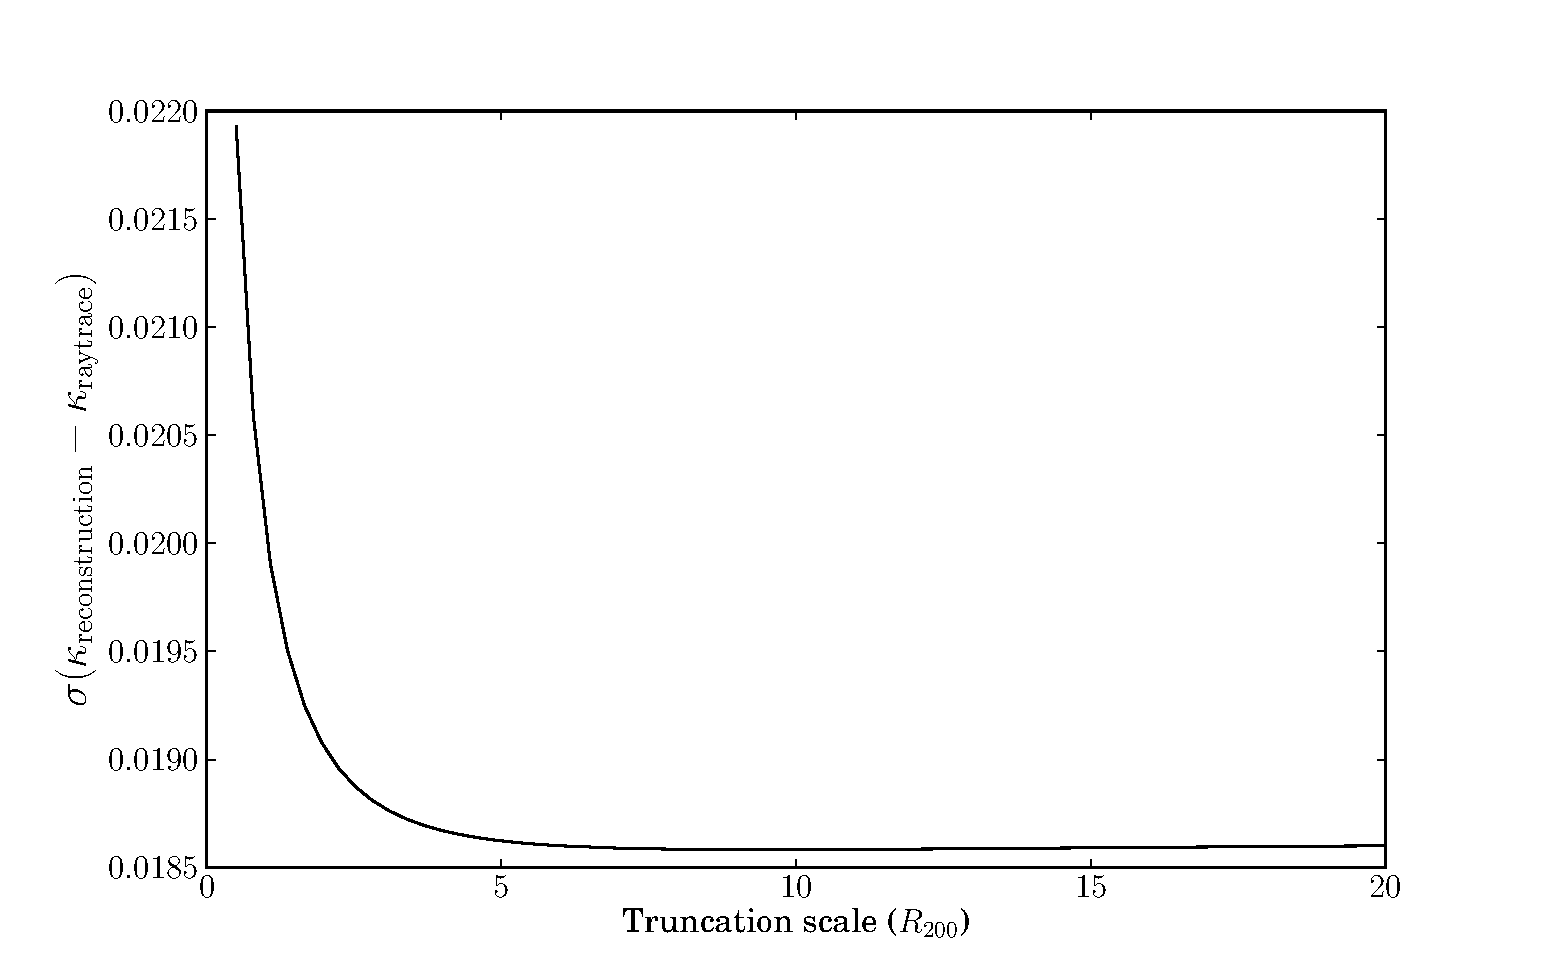
\includegraphics[width=\columnwidth]{figs/truncation_scatter.eps}
\caption[magcut]{The standard deviation in $\kapparec$ minus $\kapparay$ as a function of halo truncation radius in virial radii, using the truncated NFW profile of \citet{BMO}. In our models we truncate our halos at 5$R_{200}$}
\label{fig:ScattervsTruncation}
\end{figure}

For $\sumkappah$ to provide useful constraints on $\kapparay$, it is important that $\kapparay$ and $\sumkappah$ are as similar as possible. Figure \ref{fig:bias} shows that indeed $\sumkappah$ is a good estimator, regardless of the individual value of $\sumkappah$. At fixed $\sumkappah$ we find that the scatter in $\kapparay$ grows with $\sumkappah$; our reconstruction is better at reproducing underdense lines of sight than overdense lines of sight.

\begin{figure}
% 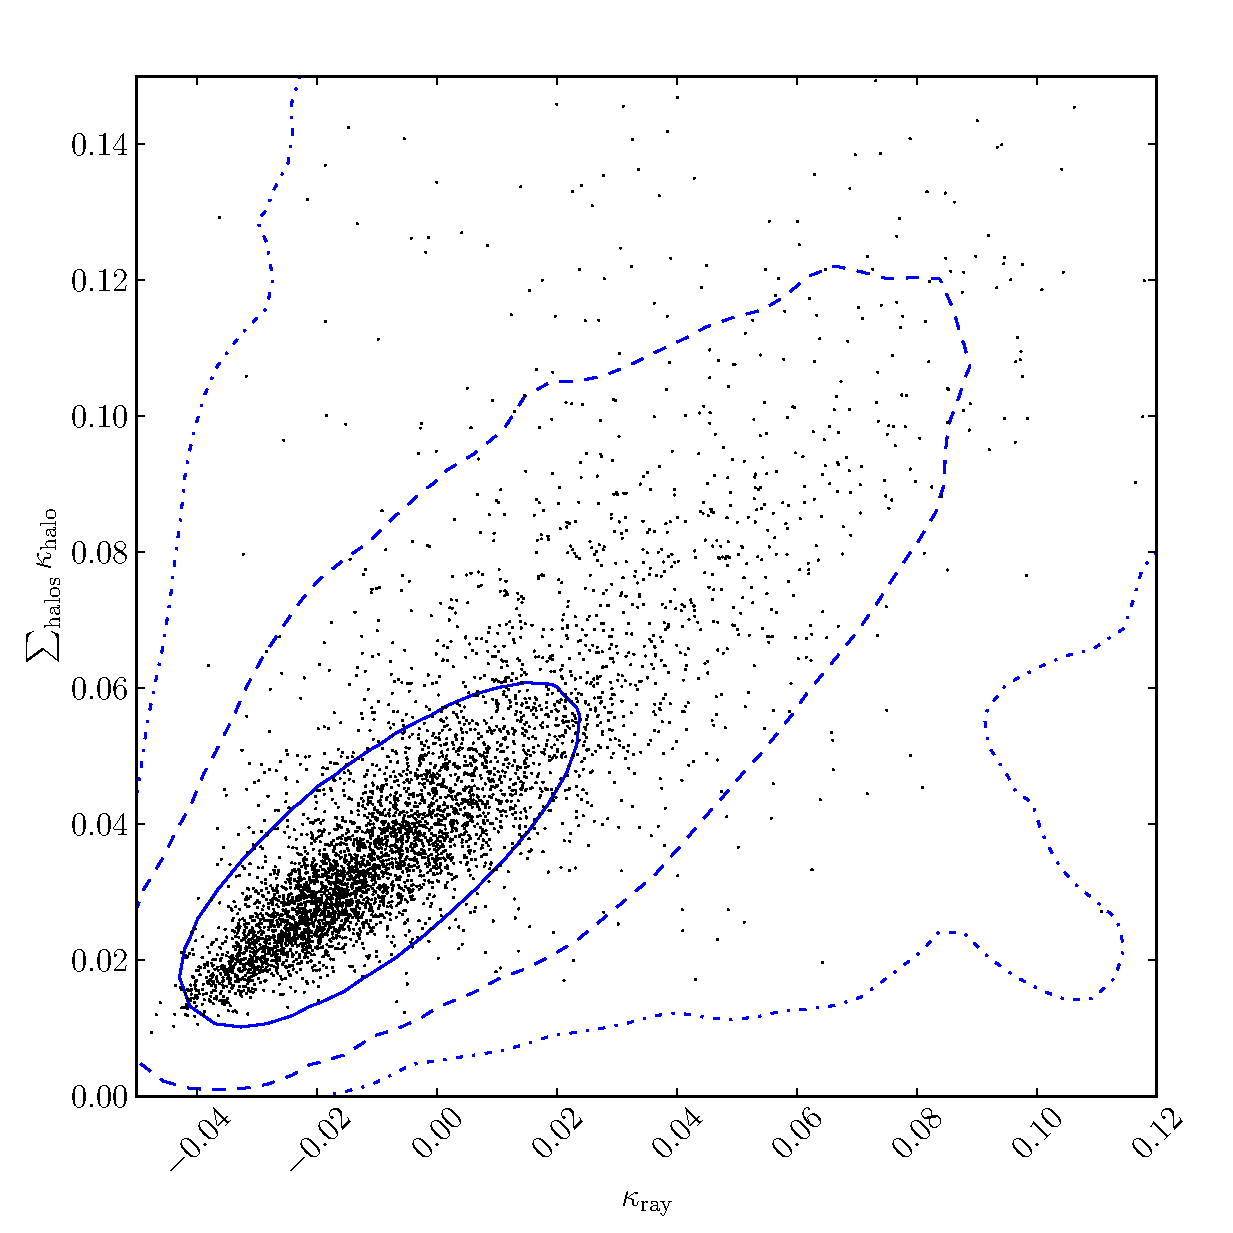
\includegraphics[width=\columnwidth]{figs/perfectc.eps}
\caption[Biased?]{$\sumkappah$ verses $\kapparay$ for 100000 reconstructed lines of sight. $\sumkappah$ traces $\kapparay$, but with a non-zero offset which is due to the negative connvergence from voids. At fixed $\sumkappah$ the scatter in $\kapparay$ grows with $\sumkappah$.}
\label{fig:isitbiased}
\end{figure}

The intrinsic error between the results of the halo based prescription and the raytraced convergence is an unavoidable error, even with perfect knowledge of halo mass and position. Before investigating the errors caused by imperfect knowledge of halo mass and redshift, we investigate the errors induced by a magnitude limited reconstruction and a field of view limited reconstruction. The halos in our catalogue are given magnitudes by the semi-analytic model of \citet{deLucia+Blaizot2007} and by applying magnitude cuts to our catalogue, we can investigate the scatter caused by unobserved halos. The majority of the convergence comes from halos with an $i$ magnitude between 18 and 24. Figure \ref{fig:magcut} shows that the width of $\kapparec-\kapparay$ decreases quickly between $i=18$ and $i=24$. Objects brighter than $i=18$ are either too rare or too close to the observer to make a significant contribution to the convergence. Objects fainter than $i=24$ are too small to be important, unless they are extremely close to the line of sight where it is likely that neglecting stellar mass and using a spherical NFW prescription are too naive to adequately reconstruct $\kappax$. It is likely that ultra-faint halos (or substructures), the uncertain contribution of voids and halos deviating from our spherical truncated NFW profile are the three major sources of the scatter in $\kapparec-\kapparay$; a deeper survey will not be sufficient to decrease the size of this scatter. Since a large number of callibration lines of sight must be reconstructed to sample $\pr(\kappav)$, it may prove unrealistic to reconstruct the calibration lines of sight out to 5 arcminutes. Figure \ref{fig:radcut} shows the width of $\kapparec-\kapparay$ as a function of reconstruction radius; in almost all cases there is no significant contribution to $\kappa$ from halos that are centred more than 1 arcminute away, although large groups or clusters can sometimes still make a contribution as far out as four arcminutes. For the rest of this work we will continue to model all of the halos out to 5 arminutes with an $i$ magnitude greater than 26, although a reconstruction with fields going out to two arcminutes and down to $i=24$ would do almost as well.

\begin{figure}
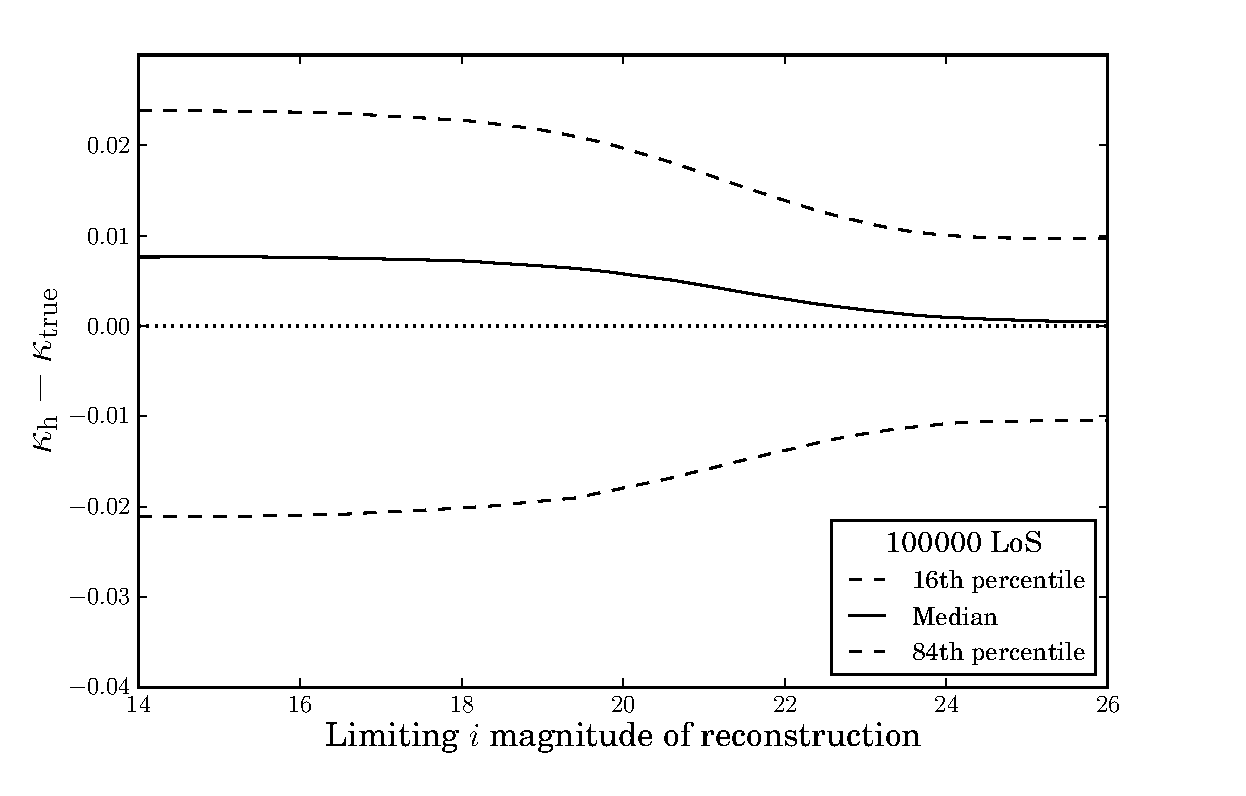
\includegraphics[width=\columnwidth]{figs/mag_scatter.eps}
\caption[magcut]{The 16, 50 and 84\% confidence intervals on $\kapparec$ minus $\kapparay$ as a function of the limiting $i$ band depth of the halo reconstruction. $\kapparec$ is given by $\sumkappah-\kappav$, where $\kappav$ is a constant such that $\left\langle\kapparec\right\rangle=0$. The majority of the constraining power comes from reconstructing halos with magnitudes between $18<i<24$}
\label{fig:magcut}
\end{figure}
\begin{figure}
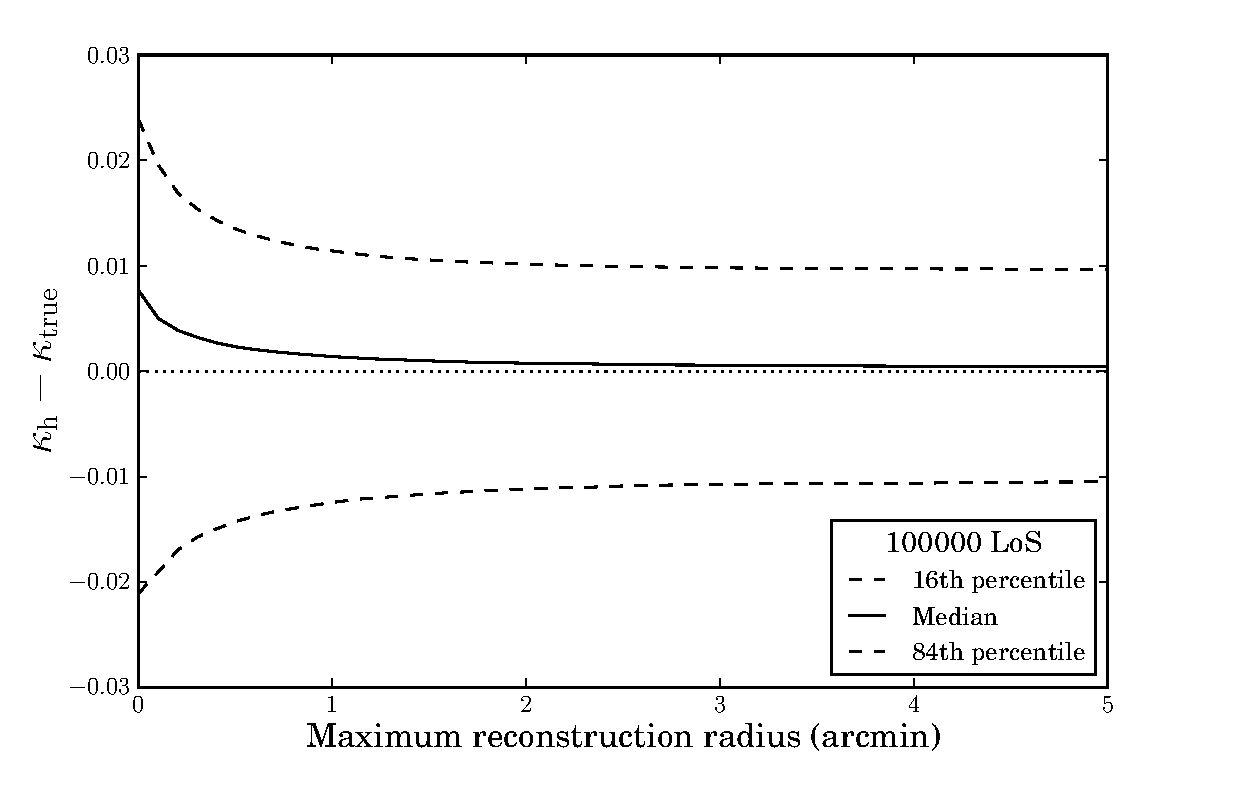
\includegraphics[width=\columnwidth]{figs/radius_scatter.eps}
\caption[radius cut]{The 16, 50 and 84\% confidence intervals on $\kapparec$ minus $\kapparay$ as a function of the limiting radius (in arcminutes) beyond which halos are not reconstructed. The majority of the convergence comes from halos centred within an arcminute of the line of sight}
\label{fig:radcut}
\end{figure}

The final test that we apply to the perfect knowledge reconstruction is to apply the marginalization outlined in Section \ref{subsec:voids}. Taking the reconstructed $\sumkappah$ for $1\times 10^{5}$ lines of sight we form the joint distribution, P$(\kapparay,\sumkappah)$ and marginalize over all sightlines with a similar $\sumkappah$ to give P($\kappax$). We define the bias as the difference between the expectation value of $\kappax$ and the known true value of $\kapparay$ for each Line of sight and we define the reconstruction width as half the width of the interval containing the central $68\%$ of the probability P($\kappax$). From $1\times 10^{4}$ reconstructed lines of sight we find the the bias to have mean of $-9.5\times 10^{-6}$ and a mean reconstruction width of 0.0132. In the case where one assumes P$(\kappax)$ is given by the global P$^{\rm global}(\kappax)$, the same $1\times 10^{5}$ lines of sight show a mean bias of $4.3\times 10^{-5}$ and mean reconstruction width of 0.237. Within the statistical error both methods are unbiased, but for any individual line of sight the bias is typically 1.8 times smaller with the reconstructed P$^{\rm reconstruction}(\kappax)$, rather than global P$^{\rm global}(\kappax)$. 

%%%%%%%%%%%%%%%%%%%%%%%%%%%%%%%%%%%%%%%%%%%%%%%%%%%%%%%%%%%%%%%%%%%%%%%%%%%%%%%%

\section{Applying the Halo Model approximation to mock catalogs}
\label{sec:obsMstar+z}

Real attempts to reconstruct the convergence along a line of sight will not have direct access to the masses of dark matter halos, 
and will likely not have access to their spectroscopic redshift either. Instead these properties must be inferred from astrophysical
observables. In principle the only observables are astrometric positions, photometric colours and possibly spectra. In this section we
quantify the errors induced by inferring the halo mass and redshift from the observables. Much work has already focused on using
photometric colours to infer stellar mass \citep[\eg][]{xxx} and redshifts \citep[\eg][]{BPZ}, in line with these we shall use
stellar mass and photometric redshifts (with appropriate errors), as the observables that must be converted into an estimate
of $\kappax$. We will investigate two main sources of error: inferring halo mass given observed stellar mass and placing halos at the wrong redshift due to photometric redshift error.

We generate a stellar mass for each halo according to the stellar mass--halo mass relation of \citet{BehrooziEtal2010}. From this stellar mass we simulate 
an observed stellar mass by drawing a sample from $\pr(\log(M_{* \mathrm {obs}})|\log(M_{* \mathrm {true}}))$ which is given by \comments{ the product of the galaxy stellar mass function (GSMF) of \citet{Fontana2006} and} a Gaussian of width $\sigma_{M_*}$ centred on $\log(M*_{\mathrm {true}})$. Where a spectroscopic redshift exists stellar masses can be estimated with typical uncertainties of 0.15 dex \citep{xxx}, however with photometric redshifts stellar mass uncertainties are typically three times as large \citep{xxx}; we use $\sigma_{M_*}=0.15$ for halos with a spectroscopic redshift and $\sigma_{M_*}=0.45$ otherwise. \comments{The \citet{Fontana2006} GSMF is given by a Schechter function with redshift evolving parameters
\be
\label{eq:GSMF}
{\dee N \over \dee M_*} \propto \left(10^{(M_*-M_0(z))}\right)^{(1+\alpha(z))} \exp \left(-10^{(M_*-M_0(z))}\right)
\ee 
where $M_0(z)=11.16+0.17z-0.07z^2$ and $\alpha(z)=-1.18-0.082z$.} For photometric redshift errors we draw a redshift from $\pr(z_{\rm true}|z_{\rm obs})$ which we take as a Gaussian of width $0.1(1+z_{\rm spec})$ centred on $z_{\rm spec}$, where $z_{\rm spec}$ is the halo's true redshift in the \MS catalogue

For each  source of error, we reconstruct 40000 calibration lines of sight and 10000 mock lens lines of sight, following the proceedure outlined in Section \ref{sec:model}. Reconstructing the lines of sight with perfect knowledge of the redshift but an uncertain stellar mass, we find that the width of $\Pr\left(\sumkappah \right)$ grows with the expectation value of $\sumkappah$; this is not surprising since the low $\sumkappah$ lines of sight are relatively empty and so there are few opportunities for uncertainties in the halo masses to propogate into $\sumkappah$ uncertainties. After applying the void correction the expected bias from our 10000 mock lenses is $6.7\times 10^{-5}$ and the mean reconstruction width is 0.0145; this is the typical reconstruction error that could be expected from a complete spectroscopic survey of the field, it is ten percent worse than the reconstruction given perfect knowledge of the halo masses and redshifts but still 1.6 times better than using the global P$^{\rm global}(\kappax)$ although a complete spetroscopic survey is still unrealistic. The distribution of the widths of $\Pr\left(\kappax \right)$ is shown in Figure \ref{fig:width1}


\begin{figure}
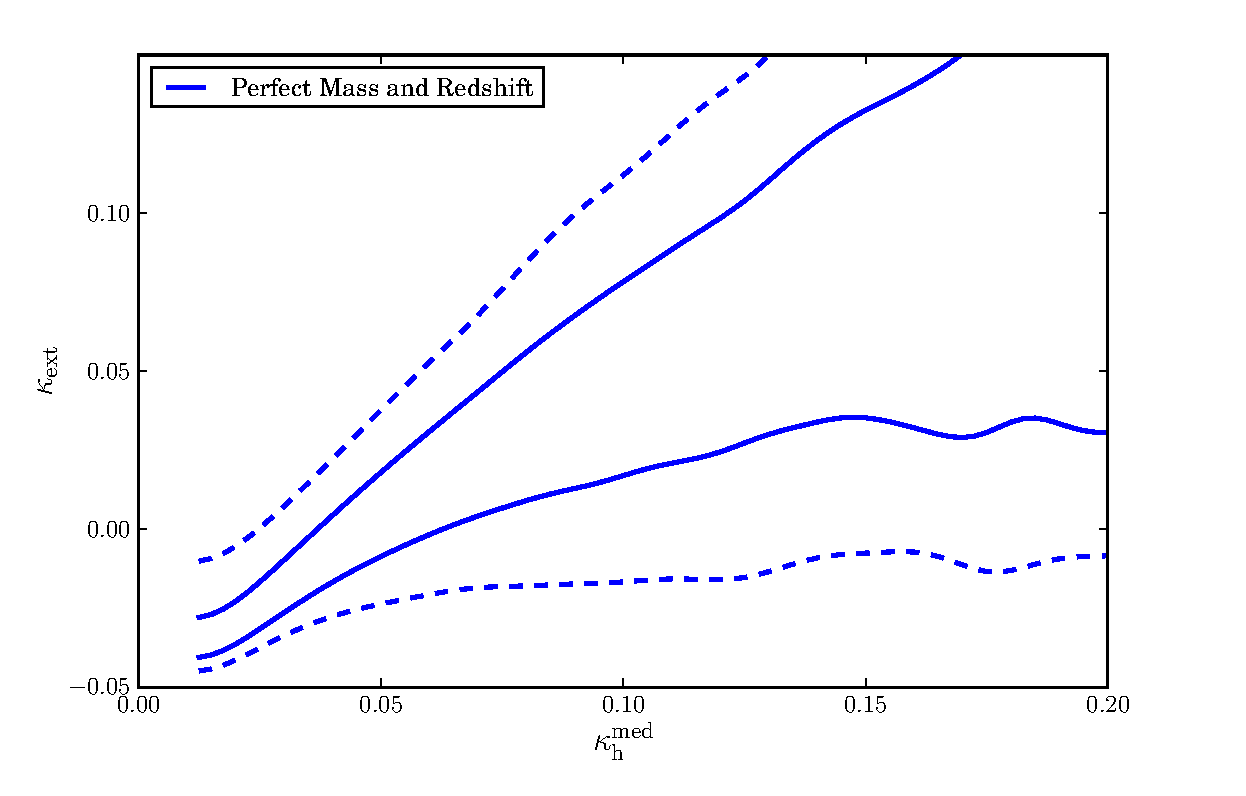
\includegraphics[width=\columnwidth]{figs/cornerplot.eps}
\caption{68 \% and 95 \% contours of the joint distribution $\pr(\kapparay, \tilde\kappa_{\rm halos})$ given a mock reconstruction of our 40000 calibration lines of sight. $\tilde\kappa_{\rm halos}$ is the median of $\pr(\sumkappah)$ given a spectroscopic redshift for each halo. $\kapparay$ and $\tilde\kappa_{\rm halos}$ are strongly correlated, despite the blurring effect of uncertain halo masses.}
\label{fig:corner}
\end{figure}

\begin{figure}
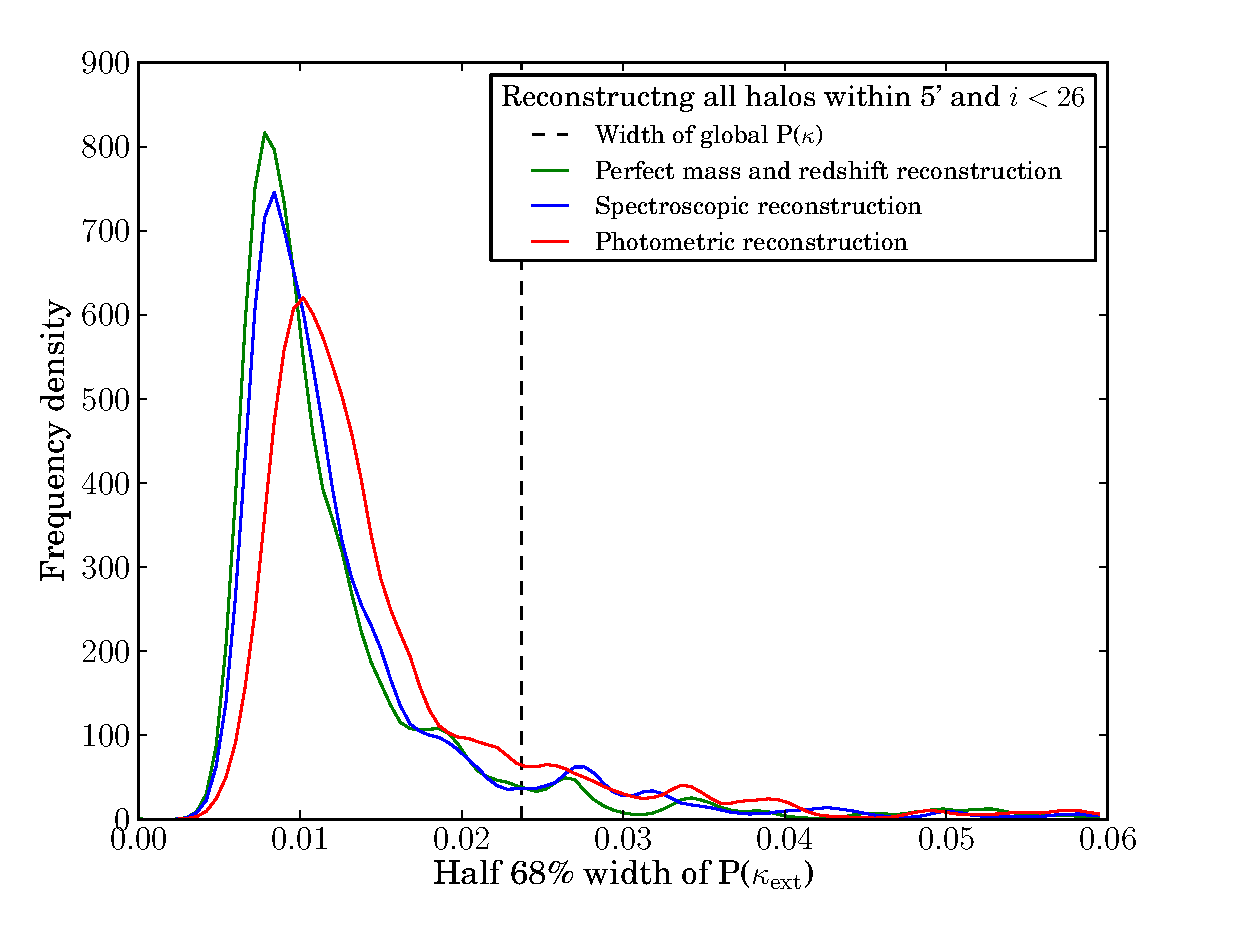
\includegraphics[width=\columnwidth]{figs/widths.eps}
\caption{Widths of $\pr(\kappax)$ after applying our reconstruction of all halos down $to i=26$ and within 5 arcminutes of the line of sight. Results for 10000 lines of sight are shown. Green is for a reconstruction given perfect knowledge of halo mass and redshift, blue is for a reconstruction given a spectroscopic redshift for every halo, and red is for a reconstruction with photometric redshifts only. The dashed black line shows the width of the global $\pr(\kappax)$ distribution; the reconstruction process provides roughly a factor of 2 improvement for the majority of lines of sight. Spectroscopic redshifts improve the reconstruction, but at signifcant observational cost.}
\label{fig:width1}
\end{figure}

Inferring the stellar mass of a galaxy from its magnitude and colours requires an estimate of how far away the galaxy is; without a spectroscopic redshift the the infered stellar mass is less precise. In principle the photometric redshift is correlated with the infered stellar mass, however we do not model this effect since the convergence from the outskirts of an individual halo is only weakly dependant on redshift at fixed mass: the redshift error is small effect on the recovered $\pr(\kappa)$ when compared to the effect of uncertain stellar masses.  With only photometric redshifts the uncertainty on $\sum\kapparec^{\rm halos}$ is much larger than the spectrocopic case, but this does not propogate into a much larger bias after applying the void correction; with a purely photometric reconstruction of the 10000 mock lightcones the results have a mean bias of $1.1\times 10^{-4}$ and a mean width of 0.0158. On average a purely photometric reconstruction of the field gives an unbiased $\pr(\kappax)$ that is 1.5 times tighter than assuming the global $\pr^{\rm global}(\kappax)$. 


%\subsection{Reconstructions of Smaller and Shallower Fields}

\begin{figure}
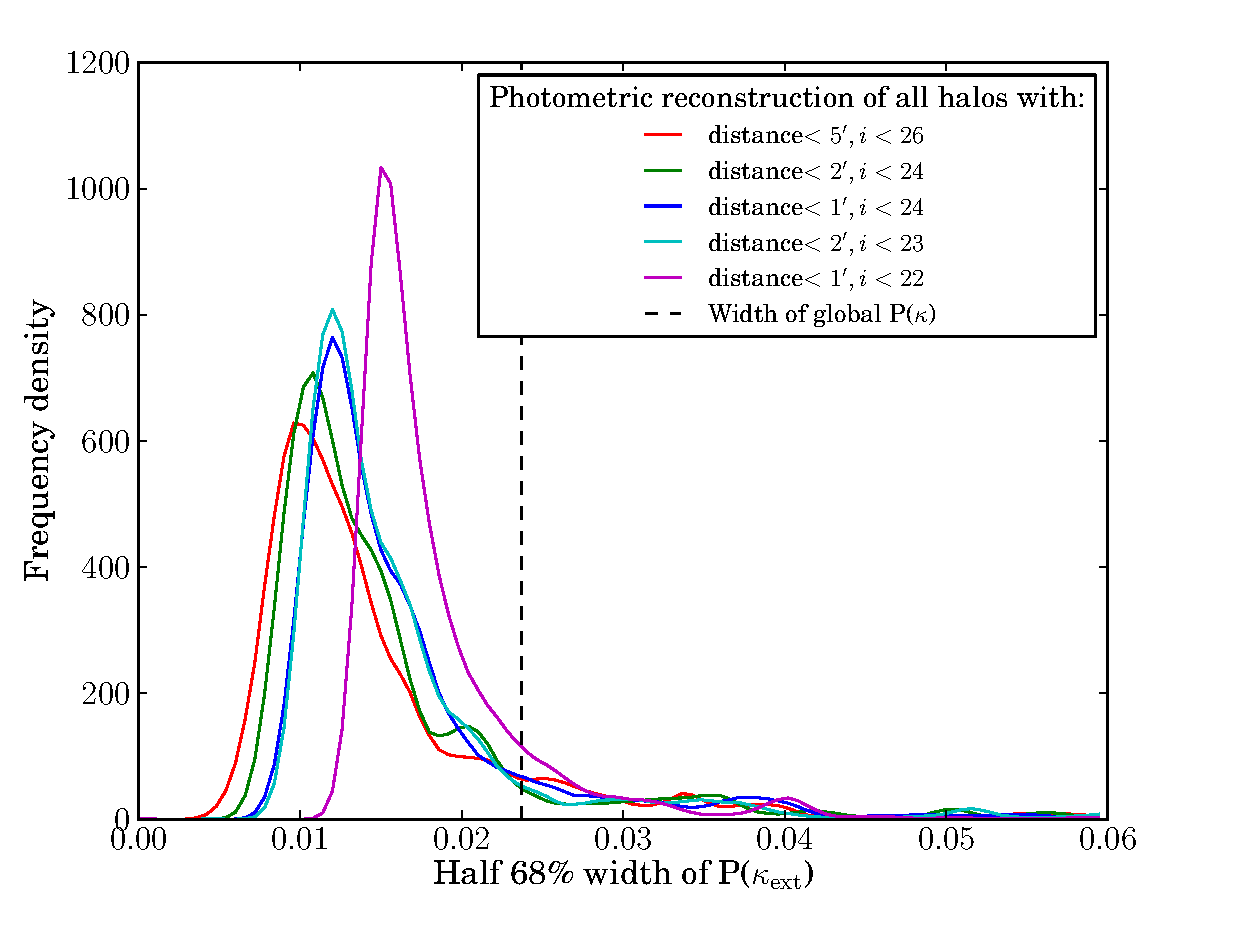
\includegraphics[width=\columnwidth]{figs/widths2.eps}
\caption{Widths of $\pr(\kappax)$ after a photometric reconstruction of all halos within different fields. The different field sizes and depths are given in the legend. As the field becomes smaller or shallower, fewer halos are being reconstructed and so the width of $\pr(\kappax)$ grows.}
\label{fig:width2}
\end{figure}


Reconstructions of real lines of sight may not have access to the deep, large calibration fields that we have used upto this point. We can perform the same reconstruction but for a more modest mock survey. Given the results of Section \ref{sec:knownMh+z} we predicted that a reconstruction of the field out to 2 arcminutes and a magnitude limit of $i$=24 would provide similar constraints to a reconstruction going out to 5 arcminutes and going down to $i$=26. We find the mean reconstruction width to be 0.0163 for a photometric reconstruction of all the halos within 2 arcminutes that have $i<24$, this is only marginally worse than 0.0158 which was the typical width after the deeper and wider reconstruction of the previous section. The reconstruction widths for our 10000 mock lens lines of sight are shown in Figure \ref{fig:widths2}. If only photometry for halos with $i<24$ and within 1 arcminute of the line of sight is availble then the typical width of the reconstructed $\pr(\kappax)$ is 0.173. Whilst a complete spectroscopic survey of a large field would be unlikely, a hybrid strategy of obtaining spectra for a subset of objects may be feasible. Photometric redshifts are sufficient to asertain the halos which are likely to contribute most of the convergence on any given line of sight, and on average there are only $\sim 6 \pm 6$ halos per line of sight that individually contribute more than 0.002 to $\sumkappah$. We investigate a hybrid strategy of obtaining spectroscopic redshifts for all of the $i<24$ halos which contribute an individual $\kappa$ of at least 0.002 combined with a photometric redshift for all other $i<24$ halos within 2 arcminutes. For the hybrid strategy the typical width of the reconstructed $\pr(\kappax)$ is 0.0151. The observational cost of obtaining spectroscopic redshifts for several 24th magnitude galaxies may make the hybrid strategy unlikley, but obtaining photometry of a 4$\times$4 arcminute patch of sky down to $i=24$ is fast with modern telescopes. The mean reconstruction width for a photometric reconstruction of all the halos within 2 arcminutes that have $i<24$ represents an improvement of 1.5 over using the global $\pr(\kappax)$ and should be achievable at minimal observational cost.


%%%%%%%%%%%%%%%%%%%%%%%%%%%%%%%%%%%%%%%%%%%%%%%%%%%%%%%%%%%%%%%%%%%%%%%%%%%%%%


\section{Testing for Systematic errors}
\subsection{Using the wrong M$_{\rm halo}$-M$_{*}$ relation}
\subsection{Selecting bias from a subset of lines of sight?}
\subsubsection{Selecting only the lines of sight with tight $\pr(\kappax)$}
\subsubsection{Selecting only high shear lines of sight}

%%%%%%%%%%%%%%%%%%%%%%%%%%%%%%%%%%%%%%%%%%%%%%%%%%%%%%%%%%%%%%%%%%%%%%%%%%%%%%
\comments{

\subsection{Comparison with Other Treatments of $\kappax$}
\label{sec:Dt:selection} 

\phil{How does distance accuracy compare with simple averaging? eg assuming
$\kappax = 0$ for all lenses. How does it compare with the no data situation?
eg where the intrinsic distribution of kappa is used as $Pr(\kappax)$.}

What is the expected bias and scatter (centroid position and width) of P(D) as a
function of N lenses? How does reconstruction compare with P(D) derived using
P(kappa|N45) for each lightcone? How does reconstruction compare with P(D)
derived assuming kappa=0 for each lightcone?

Also: compare with simple averaging. This will fail if lenses are selected to
live on over-dense lines of sight. Stefan's plot in Suyu et al shows effect of
selection - what is the resulting bias? Few percent? This is the target to beat,
need to find it out.

\subsection{Improving the Accuracy with More Information}
\label{sec:Dt:selection} 

\phil{How does distance accuracy improve with:}
\begin{itemize}
\item Spectroscopic coverage? For galaxies above some mlim? For targets with
high kappa contribution (based on photometry)?
\item IR coverage for all objects? Improves photo-z and Mstar.
\item Including shear information from lens model? Assume accurate but
uncertain extertanl shear.
\end{itemize}
}
%%%%%%%%%%%%%%%%%%%%%%%%%%%%%%%%%%%%%%%%%%%%%%%%%%%%%%%%%%%%%%%%%%%%%%%%%%%%%%

\section{Discussion}
\label{sec:discuss}

We have shown that reconstructing the matter due to halos along any line of sight can give meaningful and unbiased constraints on the external convergence along that line of sight. The total convergence along a line of sight is strongly correlated with the reconstructed $\sumkappah$. However since our model ignores voids and assumes all halos follow a spherical truncated-NFW profile our model does not include all of the relevant physics, hence the width of our resulting $\pr(\kappax)$ is still typically $\sim$0.01, even with a perfect knowledge of every halo's virial mass and redshift. To make further progress a more advanced treatment of both voids and halos will be necessary. Interestingly, we have found that the most empty lines of sight can be reconstructed with the most precision. $\kappax$ for empty lines of sight have little contributions from halos and a large contribution from voids; since they have the tightest PDFs after the reconstruction it seems that our model's biggest uncertainties are driven by naively reconstructing halos rather than neglecting voids. With a photometric reconstruction of the field there is only a small broadening compared to the perfect knowledge reconstruction; it seems that deviations from sphericity and dark matter clumping within the main halo are the dominant uncertainies rather than uncertainties in the halo mass. Inferring halo ellipticity and dark matter clumping will likely always remain a difficulty for line of sight reconstruction; as Figures \ref{fig:magcut} and \ref{fig:width2} show observing deeper than 24th magnitude does not signifcantly help the reconstruction. Because our reconstruction is mostly limited by the model, spectroscopic coverage can only provide a modest improvement to the reconstruction and at significant observational cost.

For a small fraction of lines of sight, $\pr(\kappax)$ remains very broad even after applying our reconstruction; these lines of sight are typically the most overdense lines of sight in the universe. For time-delay cosmography the most observationally expensive task is the lightcurve monitoring, whilst making photometric observations of a 4$\times$4 arcminute patch of sky survey down to 24th magnitude is a relatively cheap. We have shown that with a single epoch observation of the region around a strong lens it is possible to infer $\pr(\kappax)$. If a line of sight has a broad $\pr(\kappax)$ it can be rejected {\it before} the investment of longterm lightcurve monitoring.

The method we have outlined can also be used to estimate the external shear
along a line of sight. Shear is an observable that can be extracted from
strong lens modelling, however there is a degeneracy between internal and
external shear. Progress has been made in disentangelling external and
internal shear \citep[\eg][]{xxx} but there are still significant
uncertainties: \citet{WongEtal2011} attempted to match the shear from strong
lens models with a reconstruction of the local lens group environment, but
found a tension between the strong lens model and the reconstruction of the
environment. Since \citet{WongEtal2011} only reconstructed the local lens
group, rather than the full line of sight contribution, it is unclear whether
the external shear from lens models can be reconciled with a line of sight
reconstruction. {\it If} external shear can be measured, it provides an
additional constraint on which of the Millenium Simulation lines of sight are
similar to the reconstructed line of sight. \citet{SuyuEtal2012} found that
for RXJ1131 combining shear constriants with galaxy number count overdensity,
gave a significantly different $\pr(\kappax|\gamma,N_{45})$ copmpared to the
PDFfrom number count overdensity alone, $\pr(\kappax|N_{45})$. 



%%%%%%%%%%%%%%%%%%%%%%%%%%%%%%%%%%%%%%%%%%%%%%%%%%%%%%%%%%%%%%%%%%%%%%%%%%%%%%

\section{Conclusions}
\label{sec:conclude}

In this work we have investigated a simple halo model prescription for
reconstructing all the mass along a line of sight to an intermediate redshift
source. We have used the ray-traced lensing convergence along lines of sight
through the Millenium Simulation to test this approach, and to calibrate
estimates of the total convergence along a line of sight to an observed
distant galaxy made by summing the convergences due to each object in a
photometric catalogue. Having found that the reconstruction process is effective given perfect
knowledge of halo mass and redshift, we investigated the effects of reasonable
uncertainties in the stellar mass and redshift of each halo, and propogated
these uncertainties into a $\pr\left(\sumkappah\right)$ for each line of
sight. We draw the following conclusions:

\begin{itemize} 

\item Our model uses a truncated spherical NFW profile for
each dark matter halo and neglects voids, but despite the model's simplicity
the reconstructed $\sumkappah$ is a good tracer of $\kappax$.  We found that
with perfect knowledge of the halo mass and redshift (from the Millenium
Simulation catalogs), the reconstruction gives an unbiased estimate of
$\pr(\kappax)$ for a single line of sight that is almost almost a factor of 2
less broad than the global $\pr(\kappax)$. 

\item  For the most overdense lines of sight, the reconstruction produces a
very broad PDF, but since the reconstruction can be performed before follow-up
time is invested it will be possible to discard the most uncertain lines of
sight and prevent the waste of follow-up time. 

\item With complete spectroscopic redshift coverage and just an empirical
stellar mass to halo mass relation, we find that the median of
$\pr\left(\sumkappah\right)$ is a useful indicator for generating an estimate
of $\pr(\kappax)$ from the ensemble of simulated lines of sight. The resulting
PDF tends to be around 10\% broader than it would have been given perfect
knowledge of both halo mass and redshift; given only photometric redshifts
(which in turn give rise to much less certain stellar masss estimates) causes
another $\sim$10\% increase to the width of $\pr(\kappax)$.

\item It is very rare for halos further than 2 arcminutes to make a
significant contribution to $\kappax$. We also found that including halos
whose host galaxy is less luminous than $i=24$ does not significantly improve
our reconstruction proceedure. A photometric survey to this depth of a
4$\times$4 arcminute patch around the lens would approach the limiting
uncertainties of our simple reconstruction recipe, and yield a 
$\pr(\kappax)$ that has, on average, a width of 0.0163 --
50\% less broad than the global $\pr(\kappax)$.

\item We find that the lines of sight with the sharpest $\pr(\kappax)$ are
typically under-dense. With a photometric reconstruction of all lens fields,
and following up only the lenses with the most constraining $\pr(\kappax)$,
the width of the dominant statistical uncertainty in time-delay cosmography
can be halved, whilst at the same time decreasing any potentail for a
systematic error due to lenses being biased in $\kappax$.

\end{itemize}

\todo{Tom}{Add more conclusions about bias in a large sample of lenses...}

\todo{Tom}{Wrap up}


%Our conclusions can be summarised as follows:
%\begin{itemize}
%\item With perfect 
%\item And we found this too.
%\end{itemize}

% \item Faint galaxies and other dark structures will not appear in a photometric
% object catalog, but they will contribute convergence at some level. How much of
% the total external convergence in a time delay lens system comes from visible
% galaxies? How does this change as a function of magnitude cut? 

% \item Can the true (ray-traced) convergence be recovered by halo model
% reconstruction, and with what scatter and residual bias? Which aspects of the 
% model dominate these uncertainties?

% \item When faced with a newly-detected lens, surrounded by galaxies on the sky,
% we have some choices to make when planning follow-up observations.
% Which are the most important galaxies, with regard to the external convergence
% produced? Can nearby groups and clusters be straightforwardly accounted for? If
% lenses with such massive structures nearby are discarded, what impact does that
% have on the distance accuracy?



%%%%%%%%%%%%%%%%%%%%%%%%%%%%%%%%%%%%%%%%%%%%%%%%%%%%%%%%%%%%%%%%%%%%%%%%
%%  ACKNOWLEDGMENTS
%%%%%%%%%%%%%%%%%%%%%%%%%%%%%%%%%%%%%%%%%%%%%%%%%%%%%%%%%%%%%%%%%%%%%%%%

\section*{Acknowledgments}
 
TC thanks Vasily Belokurov for guidance and discussions.
We thank Risa Wechsler and Peter Behroozi for useful discussions and 
suggestions.
TEC acknowledges support from STFC in the form of a research studentship.
%
PJM was given support by the Kavli Foundation and the Royal 
Society, in the form of research fellowships.
%
MWA \ldots
%
SH \ldots
%
SHS \ldots
%
TT acknowledges support from the NSF through CAREER award NSF-0642621,
and from the Packard Foundation through a Packard Research Fellowship.
% 
LVEK acknowledges the support by an NWO-VIDI programme subsidy
(programme number 639.042.505).
%
This research is supported in part by the National Science Foundation under
Grant No. PHY99-07949.



%%%%%%%%%%%%%%%%%%%%%%%%%%%%%%%%%%%%%%%%%%%%%%%%%%%%%%%%%%%%%%%%%%%%%%%%%%%%%%
%  APPENDICES
%%%%%%%%%%%%%%%%%%%%%%%%%%%%%%%%%%%%%%%%%%%%%%%%%%%%%%%%%%%%%%%%%%%%%%%%%%%%%%

\appendix

%%%%%%%%%%%%%%%%%%%%%%%%%%%%%%%%%%%%%%%%%%%%%%%%%%%%%%%%%%%%%%%%%%%%%%%%%%%%%%

\section{Truncated NFW halos}
\label{appendix:halos}

 Defining $x$ as the dimensionless projected radial distance $R/r_{s}$ and $\tau$ as the dimensionless truncation radius $r_{t}/r_{s}$, \citet{BMO} derives the projected mass density, which is given by:
\begin{align}\label{eq:kappaBMO}
\Sigma_{\rm}(x) = {2\tau^2 \over (\tau^2+1)^2}\left(
        {\tau^2+1\over x^2-1}\left(1-\mathcal{F}(x)\right)
        +
        2\mathcal{F}(x)\right.\nonumber\\
        -
        \left. {\pi \over \sqrt{\tau^2+x^2}}
        +
        {(\tau^2-1)\mathcal{L}(x,\tau)
        \over
        \tau\sqrt{\tau^2+x^2}}\right)
\end{align}
where $\mathcal{F}(x)$ and $\mathcal{L}(x,\tau)$ are defined as
\be\label{eq:F} 
\mathcal{F}(x) \equiv \begin{cases}  \frac{{\rm cos}^{-1} (1/x)}{\sqrt{x^2-1}} \hspace{0.2cm} & (x>1) \\
\\
\frac{4-x^2}{3}  & (x=1)\\
\\
\frac{ {\rm cosh}^{-1} (1/x)}{\sqrt{1-x^2}} & (x<1)
\end{cases}
\ee
\be\label{eq:L}
\mathcal{L}(x,\tau) = \ln\left(\frac{x}{\sqrt{\tau^2+x^2}+\tau}\right)
\ee
%the convergence is given by $\Sigma_{\rm BMO}(x) / \Sigma_{\rm cr}(z)$.



%%%%%%%%%%%%%%%%%%%%%%%%%%%%%%%%%%%%%%%%%%%%%%%%%%%%%%%%%%%%%%%%%%%%%%%%%%%%%%

\section{Inferring $\Mhalo$ given a noisy measurement of $\Mstarobs$}
\label{appendix:MSMH}

Given a noisy estimate of the stellar mass $\Mstarobs$ of a galaxy at redshift
$z$, how can we infer the galaxy's halo mass? We then seek the posterior
PDF $\Pr(\Mhalo|\Mstarobs)$, which can be expanded as follows:

\begin{eqnarray}
&& \Pr(\Mhalo|\Mstarobs,z) = \notag\\
&& \int d\Mstar \Pr(\Mhalo|\Mstar,z) \Pr(\Mstar|\Mstarobs,z), \notag\\
&\propto& \int d\Mstar \Pr(\Mstarobs|\Mstar) \Pr(\Mstar|\Mhalo,z) \Pr(\Mhalo|z),
\label{eq:mhalo-mstar}
\end{eqnarray}
where we have used Bayes' Theorem twice to replace
$\Pr(\Mhalo|\Mstar,z) \Pr(\Mstar|z)$ with 
$\Pr(\Mstar|\Mhalo,z) \Pr(\Mhalo|z)$, and 
to invert $\Pr(\Mstar|\Mstarobs)$ into the sampling
distribution $\Pr(\Mstar|\Mstarobs)$, which we recognise as the likelihood
function for the observed stellar mass. Note that the ``true'' $\Mstar$ of the
galaxy is marginalised out: we are only interested in reconstructing the halo
mass. The last two terms in
\eqref{eq:mhalo-mstar} are the $\Mstar-\Mhalo$ relation from
\citet{BehrooziEtal2010}, and the halo mass function $\Pr(\Mhalo|z)$, at the
given redshift. We can
tabulate the product of these two from our Millenium Simulation catalog,
constructing a two-dimensional histogram of halo masses and their associated
true stellar masses (drawn from the Behroozi relation). 

For each galaxy, we compute the likelihood function for its $\Mstarobs$ as a
function of the unknown $\Mstar$, and multiply it by our tabulated joint PDF.
This heavily downweights halos with $\Mstar$ values outside the observed
range. We then do the marginalisation integral by Monte Carlo, drawing
(two-dimensional) sample parameter vectors
from the downweighted histogram, discarding the $\Mstar$ values, and
constructing a one-dimensional histogram that is an estimate of
$\Pr(\Mhalo|\Mstarobs)$.

\todo{Matt}{Edit the above text to add a note on how we do the sampling in
practice, via the CDF.}

If the redshift of the galaxy is uncertain, we need to take this uncertainty
into account; for example, for each sample drawn from the photometric redshift
posterior PDF $\Pr(z|{\rm colors})$, we can draw a sample $\Mhalo$ using the
above procedure.


%%%%%%%%%%%%%%%%%%%%%%%%%%%%%%%%%%%%%%%%%%%%%%%%%%%%%%%%%%%%%%%%%%%%%%%%%%%%%%

\section{Accounting for uncatalogued low mass halos, and voids}
\label{appendix:smooth}

Our halo model allows us to infer a halo mass $\Mhalo$ for each galaxy in a
photometric catalog; under the weak lensing approximation described in
\Sref{sec:theory} we can compute the contribution of each of these halos to
the overall convergence and shear amplitude, assuming a homogeneous
Friedman-Robertson-Walker metric and the concordance $\Lambda$CDM cosmological
parameters for the angular diameter distances to calculate the critical
density for each lens plane. Clearly this approach will tend to over-estimate
the convergence, since we are placing massive halos into a volume that has
already been assumed to be full of homogeneously distributed matter with the 
mean cosmological density. In practice, the space between massive halos will
contain a) low mass halos that are not bright enough to be detected and b)
empty space where the density is below that of the mean. A rigorous treatment
of this complex situation is beyond the scope of this paper, but is being
investigated (Blandford et al, in preparation). In this appendix we describe
our empirical approach to accounting for the missing mass and voids. 

Let the summed convergence due to halos in our galaxy catalog be $\kappah$.
Given some assumptions about halo density profile and shape, this parameter
can be inferred from a set of uncertain halo mass estimates (which have in
turn been inferred from noisy measurements of galaxy redshift and stellar mass
as described in \Aref{appendix:MSMH}). We assume each halo to be a
spherically-symmetric NFW profile, and neglect the contribution of the stellar
mass to the convergence. The halo mass inference for the $k^{\rm th}$ galaxy 
is stored as a list of sample values of $\Mhalok$ drawn from the posterior PDF
$\Pr(\Mhalok|\Mstarobsk,z_k)$; computing the contribution to the convergence
due to this halo at the target line of sight for each sample gives, in turn, 
a set of
samples drawn from the PDF $\Pr(\kappahk|\Mstarobsk,z_k)$. We then generate
samples from $\Pr(\kappah|\{\Mstarobsk,z_k\})$ by drawing a sample $\kappahk$
for each halo, summing over halos to get $\kappah$, discarding those
samples and moving down the lists.

The PDF $\Pr(\kappah|\{\Mstarobsk,z_k\})$ will, in general, be broad (due to
the uncertainties involved in halo mass estimation). It will also be shifted
towards high values of convergence, due to the FRW approximation described
above. What we really want is an inference of $\Pr(\kappa|\{\Mstarobsk,z_k\})$
instead. We can obtain this by considering the expansion:
\begin{equation}
\Pr(\kappa|\{\Mstarobsk,z_k\}) = \int d\kappah 
   \Pr(\kappa|\kappah) \Pr(\kappah|\{\Mstarobsk,z_k\})
\label{eq:kappaconv}   
\end{equation}
The first term in the integrand relates the summed  convergence due to model
halos, $\kappah$, to the true summed convergence, $\kappa$.  In the Millenium
Simulation catalogs, we can compute a single value of $\kappah$ for each
selected line of sight from the true halo mass and redshift (and our same
assumptions of halo profile and shape), and tabulate the two-dimensional PDF
$\Pr(\kappa|\kappah)$ as a sequence of one-dimensional PDFs for $\kappa$ in a
bin at fixed $\kappah$. Note that this PDF captures the ``intrinsic scatter''
of $\kappah$ due to our assumptions about the clumpiness of mass in the
Universe; the integral combines these uncertainties with those
arising from the measurement of $\Mstarobs$ and~$z$.

For any given observed catalog then, we infer
$\Pr(\kappah|\{\Mstarobsk,z_k\})$ as described above, and then
multiply it by $\Pr(\kappa|\kappah)$; we
again do the marginalisation over $\kappah$ by Monte Carlo, drawing samples
from the two-dimensional grid and keeping only the $\kappa$ values, to form
our final result, $\Pr(\kappa|\{\Mstarobsk,z_k\})$. 
This PDF will describe, by construction, an accurate (i.e., unbiased)
measurement of $\kappa$ in the case where the Millenium Simulation halo
catalog and Behroozi et al $\Mstar-\Mhalo$ relation are themselves accurate
descriptions of galaxies and their distribution. In \Sref{sec:tests} we
investigate the amplitude of the systematic errors incurred if these
assumptions are not valid.

\todo{Matt}{Add text describing whatever sampling shortcut you derive! :-)}

% Finally, we note that \Eref{eq:kappaconv} and the method for evaluating the
% integral in it can be generalized to yield 
% $\Pr(\kappa,|\gamma||\{\Mstarobsk,z_k\})$, where $|\gamma|$ is the amplitude
% of the complex shear. The amplitude of the shear due to halos, $|\gammah|$ is
% needed in this calculation, and marginalised over -- $\gammah$ is computed by
% simple summation of its components, as in \Sref{sec:theory}. In
% \Sref{sec:includinggamma} we explore the impact that knowing $\gamma$ (from,
% for example, a strong lens model)  has on the inference of $kappa$, and how
% severe the systematic errors from getting this wrong might be.


%%%%%%%%%%%%%%%%%%%%%%%%%%%%%%%%%%%%%%%%%%%%%%%%%%%%%%%%%%%%%%%%%%%%%%%%%%%%%%
%  REFERENCES
%%%%%%%%%%%%%%%%%%%%%%%%%%%%%%%%%%%%%%%%%%%%%%%%%%%%%%%%%%%%%%%%%%%%%%%%%%%%%%

% MNRAS does not use bibtex, input .bbl file instead. 
% Generate this in the makefile using bubble script in scriptutils:

% bubble -f paper-lcr.tex references.bib 
% %%%%%%%%%%%%%%%%%%%%%%%%%%%%%%%%%%%%%%%%%%%%%%%%%%%%%%%%%%%%%%%%%%%%%%%%
%
% Pangloss: Testing the reconstruction paper
%
%%%%%%%%%%%%%%%%%%%%%%%%%%%%%%%%%%%%%%%%%%%%%%%%%%%%%%%%%%%%%%%%%%%%%%%%

\documentclass[useAMS,usenatbib]{mn2e}
%% letterpaper
%% a4paper

% \voffset=-0.8in

% Packages:
\input psfig.sty
\usepackage{xspace}
\usepackage{graphicx}
\usepackage{amssymb}
\usepackage{amsmath}

% Macros:
\input{macros.tex}
\input{addresses.tex}

%%%%%%%%%%%%%%%%%%%%%%%%%%%%%%%%%%%%%%%%%%%%%%%%%%%%%%%%%%%%%%%%%%%%%%%%%%%%%%

\title[Line of Sight Mass Reconstruction]
{Inferring Lensing Mass in the Universe \\
from Photometric Catalog Data}
    
\author[Collett \etal]{%
  Thomas~E.~Collett$^{1}$\thanks{\collettemail},
  Philip~J.~Marshall$^{2}$,
  Matthew~W.~Auger$^{1}$,
  Stefan~Hilbert$^{3}$,
\newauthor{%
  Sherry~H.~Suyu$^{4}$,
  Zachary~Greene$^{4}$,
  Tommaso~Treu$^{4}$\thanks{\packard},
  Christopher~D.~Fassnacht$^{5}$,}
\newauthor{%
  L\`eon~V.~E.~Koopmans$^{6}$,
  Roger~D.~Blandford$^{3}$} 
  \medskip\\
  $^1$\ioa\\
  $^2$\oxford\\
  $^3$\kipac\\
  $^4$\ucsb\\
  $^5$\davis\\
  $^6$\kapteyn
}

%%%%%%%%%%%%%%%%%%%%%%%%%%%%%%%%%%%%%%%%%%%%%%%%%%%%%%%%%%%%%%%%%%%%%%%%%%%%%%

\begin{document}
             
\date{to be submitted to MNRAS}
\pagerange{\pageref{firstpage}--\pageref{lastpage}}\pubyear{2012}

\maketitle           

\label{firstpage}

%%%%%%%%%%%%%%%%%%%%%%%%%%%%%%%%%%%%%%%%%%%%%%%%%%%%%%%%%%%%%%%%%%%%%%%%%%%%%%

\begin{abstract} 

Strong gravitational lenses can provide high precision cosmological distance
measurements; one of the most important sources of systematic error in these
estimates is the additional mass along the line of sight to the source. Weak
lensing by galaxies and groups in this beam can contribute an ``external
convergence'' $\xkappa$ that dominates the  uncertainty in the inferred
distances; likewise, it may also contaminate estimates of the luminosity of
objects at high redshift (such as reionisation-era proto-galaxies, and type Ia
supernovae standard candles).  We characterise this uncertainty by marginalising
over a probability density function for $\xkappa$: here, we investigate the use
of a simple halo model to estimate $\Pr(\xkappa)$ given noisy estimates of the
photometric redshift and stellar mass of galaxies observed in optical imaging
surveys of the field in question. We use mock catalogs from the Millenium
Simulation and compare our reconstructed $\Pr(\xkappa)$ to ray-traced $\kappa$ values,
we find that our model produces an unbiased estimator of $\kappax$,
For each lightcone the individual $\Pr(\xkappa)$ from this reconstruction process are
typically 1.8 times narrower than the global distribution of $\xkappa$ given perfect knowledge 
of the halo mass and redshift. After incorporating uncertainties on redshift and halo and stellar masses
we typically find that the reconstruction yields an improvement factor of 1.5. For each line of sight the
 $\Pr(\xkappa)$ can be formed before the investment of light-curve monitoring. By following up only the 
most costrained lines of sight a factor of 2 improvement over the global $\pr(\kappax)$ should be 
achievable.
\end{abstract}

% Full list of options at http://www.journals.uchicago.edu/ApJ/instruct.key.html

\begin{keywords}
  gravitational lensing   --
  methods: statistical    --
  galaxies: halos         --
  gaaxies: mass function  --
  cosmology: observations
\end{keywords}

\setcounter{footnote}{1}

%%%%%%%%%%%%%%%%%%%%%%%%%%%%%%%%%%%%%%%%%%%%%%%%%%%%%%%%%%%%%%%%%%%%%%%%%%%%%%

\section{Introduction}

Averaged over large areas of sky, the weak gravitational lensing effect can be
used to constrain the statistical properties of the matter density in the
Universe: every distant object we observe has had its shape distorted, and size
and total brightness magnified (or demagnified) by a compound lens constructed
from all the mass distributed between us and it.

This fact makes weak gravitational lensing a potentially important source of
systematic error for any estimate of luminosity or distance, an issue
raised for \eg 
type Ia supernovae by \citet[][]{Holz+Wald1998,Linder+Holz2004}, for
gamma ray bursts by \citet[][]{Oguri+Takahashi2006,Wang+Dai2011}, 
and for high redshift galaxies by \citet{BradacEtal2009}, among others. 
Along lines of sight containing strong gravitational lenses,
the effect has been found to be
particularly important, with foreground and background structures
having a significant effect on the inferred lensing cross-section
\citep[\eg][]{WongEtal2012} and distance ratios \citep[][]{DalalEtal2005}.
In time delay lens cosmography,
\citet{SuyuEtal2010} found that  the lensing effect of mass structures along the
(unusually over-dense)  line of sight to the quadruply-imaged radio source
B1608$+$656, the so-called ``external convergence,'' was the dominant source
of uncertainty in their 6\% measurement of Hubble's constant. 

How can we correct for this weak lensing error, and make
accurate measurements through the Universe? When inferring global quantities
(such as the cosmological parameters), averaging the results from a large
number of independent objects will tend to reduce the error, as the
ensemble-averaged convergence approaches zero for an unbiased sample
\citep[\eg][]{Linder+Holz2004}. If the sample is biased, however, some
residual systematic error will remain while the statistical uncertainty
decreases -- and this will be the case for any sample selected by the
brightness of the lensed object, or any other quantity that depends on
$\xkappa$. The latter class includes time delay lenses, which could be
either detected or selected 
based on their image separations, magnifications or quadruple image
configurations, all of which either increase or become more likely with
increasing $\kappa$. Large
samples of lenses are expected to be discovered in the next decade in
ground-based optical imaging surveys \citep{Oguri+Marshall2010} -- but these
samples will be image separation-limited, due to the surveys' relatively poor
($\sim 1$~arcsec) image quality. Some of the current sample of known time
delay lenses were detected in surveys like this: we might expect them to be
somewhat biased towards high values of $\xkappa$.

There are two broad approaches one could take at this point. First, one could
seek to characterise the lensed objects' selection function, and use this
understanding to derive a suitable correction to cosmological parameters
inferred assuming no $\xkappa$ at all. As pointed out by  \citet[][among
others]{Oguri+Takahashi2006}, to do this one would need  information about the
unlensed population of objects, and the population of lenses, and how the
objects were detected -- or to infer these hierarchically during the analysis.
Alternatively, one could simply accept all lenses provided, regardless of
their selection, and try to use any additional information that is available
to estimate the external convergence in each system on a case by case basis,
and hence optimize their joint analysis to produce a better-constrained result
\citep[as suggested by][]{Keeton+Zabludoff2004}. In this work we follow this
second approach, and use measurements of the positions, magnitude and colours
of galaxies close to lens lines of sight to try to infer the
external convergence at the lens position. 

Attempts to date at reconstructing the local and  line of sight mass
distribution in strong lens fields (what \citeauthor{WongEtal2011} call ``the
full environment'') have focused on photometric and  spectroscopic surveys to
detect galaxy groups and ascertain galaxies' membership,  and on understanding
the external shear apparently required by the strong lens models. Surveys by
\citet{Fassnacht+Lubin2002,AugerEtal2007,WilliamsEtal2006,MomchevaEtal2006}
all found groups of galaxies both hosting and lying  along the line of sight
to known gravitational lenses. Initial estimates of the effect of these
structures suggested the importance of assigning mass to both galaxy and group
halos, and to allowing for significant uncertainty in the centroids of group
halos. The probability density function (PDF) for the external convergence for
that lens, $\Pr(\xkappa)$, is the target for any reconstruction analysis, and
is the key quantity for any ensemble analysis, since by marginalising over it
we can correctly propagate the uncertainties due to weak lensing. Coming
closest to estimating this quantity from survey data, \citet{WongEtal2011} ran
Monte Carlo reconstructions of the mass in nine lens fields based on
\citeauthor{WilliamsEtal2006} and \citeauthor{MomchevaEtal2006}'s
photometric and spectroscopic measurements of galaxies close to the line of
sight, and compared the resulting predicted shear distributions with the
external shear demanded by the strong lens model. Their simulations show most
of the shear being generated by bright galaxies within 2~arcminutes of the
lens, and that both line of sight structures and the group of galaxies in each
lens plane contribute significant proportions of the shear. They find
significant discrepancies between the lens model shear and the Monte Carlo
predictions, and are unable to distinguish between the environment modelling
and the strong lens modelling as the cause of these discrepancies.

These observational investigations have provided very useful insight into the
problem.  Coming from a more theoretical direction, large numerical
simulations have been used to predict, from first principles, the distribution
of likely external shears and convergences along strong lens lines of sight. 
\citet{Holder+Schechter2003} and \citet{Dalal+Watson2004} carried out
ray-tracing calculations in N-body simulations to estimate the  distribution
of external shear values.  \citet{HilbertEtal2009} performed similar ray-tracing
experiments through the Millenium Simulation \citep{SpringelEtal2005},
generating a predicted $\xkappa$ at every position in a simulated sky. The
first step towards using this excellent calibration resource was taken by
\citet{SuyuEtal2010}, who selected Millenium Simulation lines of sight that a)
were found to contain a strong lens and b) had comparable apparent galaxy
overdensity in a 45 arcsec radius aperture down to $i < 24$. This overdensity
could be compared to the overdensity of the B1608$+$656 line of sight
\citep{FassnachtEtal2011}, and hence an estimate of  $\Pr(\xkappa)$ could be
made. 

In this paper, we bring these observational and theoretical approaches
together and  use numerical simulations to {\it test and calibrate} a
reconstruction of the  external convergence. Ray-tracing through the
simulations gives a ``truth'' that we can attempt to recover.  In this paper
we use the Millenium Simulation mock galaxy catalogs and ray-traced lensing
effects to test the accuracy of line of sight mass reconstructions.
Probabilistically ssigning mass and redshift to every observed galaxy in the
field around a time delay lens, we generate Monte Carlo sample line of sight
mass distributions, and estimate the external convergence due to each one.
This gives us a $\Pr(\xkappa)$ that can be propagated into further joint
inferences. We focus on time delay lens cosmography, and quantify our results
in terms of the uncertainty on the mean time delay distance to a test sample
of $N$ lenses (where for clarity each lens has the same deflector and source
redshift, and the same lens model and time delay uncertainty).

We aim to answer the following questions:
\begin{itemize}
\item Faint galaxies and other dark structures will not appear in a photometric
object catalog, but they will contribute convergence at some level. How much of
the total external convergence in a time delay lens system comes from visible
galaxies? How does this change as a function of magnitude cut? 
\item Can the true (ray-traced) convergence be recovered by halo model
reconstruction? What scatter and residual bias are induced in the ensemble 
distance estimate? Which aspects of the model dominate these uncertainties? 
\item When faced with a newly-detected lens, surrounded by galaxies on the sky,
we have some choices to make when planning follow-up observations.
Which are the most important galaxies, with regard to the external convergence
produced? Can nearby groups and clusters be straightforwardly accounted for? If
lenses with such massive structures nearby are discarded, what impact does that
have on the distance accuracy?
\end{itemize}

This paper is organized as follows. In~\Sref{sec:theory} we review the relevant
gravitational lensing theory, before introducing our simple reconstruction 
model in \Sref{sec:model}.  We then test this model in two phases: first, in
\Sref{sec:knownMh+z}, with known redshift and halo mass for every galaxy in a
lens field, in order to quantify the irreducible uncertainty due to unseen mass,
and second, in \Sref{sec:obsMstar+z}, with realistic observational uncertainties
on the field galaxies' stellar masses and redshifts. \comments{We then propagate all these
uncertainties through to the time delay distance in a toy sample of 100 lenses,
in \Sref{sec:distances}.} We discuss our results in \Sref{sec:discuss} before
concluding in \Sref{sec:conclude}.

Throughout this paper magnitudes are given in the AB system and
we adopt the Millenium Simulation's ``concordance'' parameters for our reference cosmology, \ie
$h=0.73$, $\Omega_m=0.25$ and $\Omega_\Lambda=0.75$, where the symbols indicate
the Hubble Constant in units of 100 km s$^{-1}$ Mpc$^{-1}$ and the matter and
dark energy density of the Universe in units of the critical density
.%\citep[e.g.\ ][]{KomEtal09}.


%%%%%%%%%%%%%%%%%%%%%%%%%%%%%%%%%%%%%%%%%%%%%%%%%%%%%%%%%%%%%%%%%%%%%%%%%%%%%%

\section{Theoretical Background}
\label{sec:theory}

%Time delay distances, and the mass sheet degeneracy - how kappa is degenerate in
%strong lens models (and magnifications).


Convergence, or Ricci focusing, occurs when a gravitational lens focuses the rays in a raybundle.
This focussing can cause distant objects to appear brighter, and larger than they would if the lens
 were removed.
The convergence from an isolated mass sheet is the ratio of the projected surface mass density
($\Sigma(D_{\mathrm{od}}\bmath{\theta})$) devided by the critical surface mass density at the redshift of the mass sheet ($\Sigma_{\rm cr}$),
\be
\kappa(\bmath{\theta})= \frac {\Sigma(D_{\mathrm{od}}\bmath{\theta})}{\Sigma_{\rm cr}(z)}
\ee
where 
\be \label{eq:sigcrit} 
\Sigma_{\rm cr}(z) \equiv \frac{c^2 D_{\rm os}}{4 \pi G D_{\rm od} D_{\rm ds}}.
\ee
and the D's are the angular diameter distances between the objects refered to in the subscripts: o is the observer, d is the deflector and s is the source. If the surface mass density of the sheet exceeds $\Sigma_{\rm cr}$, multiple images of the source can
occur, otherwise only one image will be observed, although that image will still be perturbed
relative to the unlensed case.

Strong lensing occurs when a massive object and background source are almost perfectly
aligned along a line of sight. The light from the background source is deflected by the
lens galaxy; this deflection allows multiple images of the background source to form
at stationary points of the time delay function. For an isolated lens, the time delay
function can be calculated from
\be \label{eq:T} 
\Delta t(\bmath{\theta},\bmath{\beta}) = \frac {1}{c} \frac{D_{\rm od} D_{\rm os}}{D_{\rm ds}} (1+z_{\rm d})\, \phi(\bmath{\theta},\bmath{\beta}),
\ee
where $\bmath{\theta}$ is the observed source position, $\bmath{\beta}$ is the 
unlensed source position, $z_{\rm d}$ is the redshift of the lens, $\phi(\bmath{\theta},\bmath{\beta})$ is
the Fermat potential. The Fermat potential is given by
\be \label{eq:FP}
\phi(\bmath{\theta},\bmath{\beta})\equiv \left[\frac{(\bmath{\theta}-\bmath{\beta})^2}{2}-\psi(\bmath{\theta}) \right], 
\ee
where $\psi(\bmath{\theta})$ is the lens potential, derived from the projected dimensionless
surface mass density, $\kappa(\bmath{\theta})$, by 
\be \label{eq:psikappa}
\kappa(\bmath{\theta})=\frac{1}{2}\nabla^2\psi(\bmath{\theta}).
\ee

Strong lenses sit in our real Universe -- they are not truely isolated;
there is some mass along the line of sight coming from intervening structures.
These structures may be physically associated with the lens e.g. other members
of a group or cluster, or they may be the result of chance alignments at any redshift. 
Whilst it is rare for three galaxies to line up well enough for both of the background sources
to be strongly lensed \citep{GavazziEtal2008,CollettEtal2012a}, the shear scale of dark matter halos
makes a partial alignment -- with the additional structure acting as a weak lens -- 
a near certainty, indeed \citet{Vale+White2003} and \citet{HilbertEtal2007} find that there
are no empty lightcones in a realistic universe. These additional structures induce an external shear
which can be recovered in the mass-modelling of the lens, but they can also introduce a convergence that
is undetectable from the image positions, shapes and relative fluxes; {\it the
mass sheet-degeneracy} \citep{FalcoEtal1985}.

If the intrinsic source brightness changes, the observed brightness in each image does not change
simultaneously - there is a time delay, $\Delta t$, between the brightness change in
each image. Despite the invariance of the image positions and fluxes, under the addition
of an external convergence (and appropriate re-scaling of the lens potential) the relative Fermat potential between the images is {\it not}
invariant, and so the time delay changes. As such it is necessary to include $\kappax$
in the lens modelling, if cosmological parameters are to be estimated accurately and
precisely from observed time delays \citep{SuyuEtal2010}.

\comments{
If the mass sheet is not physically associated with the lens galaxy, it can lie at any redshift. The effects of such a mass-sheet can be projected back onto the lens plane in the form of an effective convergence. We define this effective convergence in two limits.
\begin{itemize}
\item No significant perturbations along the line of sight, and \\
\item A single dominant perturber, relative to which all other perturbations are small.
\end{itemize}
We will refer to these cases as the magnification case (subscript $\mu$ in formulae), and the strong lensing case (subscript SL in formulae), respectively. We will ignore the additional case, of a compound lens, with several significant perturbers. 

The magnification case has no primary lens plane, and is chiefly relevant for the magnifications of distant objects. In the absence of a primary lens plane, we are free to define the effective convergence on any point; the effective convergence is the same, independant of the plane choosen. It can be shown \citep[\eg][]{xxx} that if there are several mass sheets at redshifts $\{z_{p}\}$, with convergences $\{\kappa_p =\Sigma_{p}/\Sigma_{\mathrm{cr}}(z_p)\}$, the effective convergence is given by
\be \label{eq:kappasummu}
\kappa_{\mathrm{effective,\mu}}=\sum_{p}\kappa_p.
\ee

In the stong lensing case, the presence of a significant perturber alters the
geometry of the system, and provides a primary lens plane. It is the primary
lens plane upon which we need to know $\kappa_{\mathrm{effective}}$, since
this is where the mass-sheet degeneracy is defined. Following Equations 20--32
of \citet{keeton2003}\flag{keeton2003}, it can be shown that the relevant
effective convergence is given by 
\be \label{eq:kappasumSL}
\kappa_{\mathrm{effective,SL}}=
{  
(1-\beta_{12})(\kappa-\beta_{12}(\kappa^2-\gamma^2))
\over
(1-\beta_{12}\kappa)^2-(\beta_{12}\gamma)^2
}
\ee
where $\kappa$ and $\gamma$ are, respectively, the convergence and shear
caused by the perturber, in their own plane and $\beta_{12}$ is a geometrical
scaling factor defined by
\be\label{eq:beta}
\beta_{12}={
D_{12} D_{\mathrm{os}}
\over
D_{\mathrm{o}1} D_{1\mathrm{s}}
}
\ee
where the D's are again angular diameter distances: the 1 (2) in the subscript
refers to the lower (higher) redshift object of the lens and perturber. For
the case that the mass sheet is in the lens plane, $\beta_{12} = 0$ and
$\kappa_{\mathrm{eff}}=\kappa$; if the mass-sheet is in the plane of the
observer, or source, $\beta_{12} = 1$ and $\kappa_{\mathrm{eff}}=0$; for a
mass-sheet at any other redshift $0<\beta_{12}<1$. In the case of several mass
sheets the effective convergences sum. In the limit that both $\kappa$ and
$\gamma$ are small, Equation \ref{eq:kappasumSL} reduces to 
\be \label{eq:kappasumSLweak}
\kappa_{\mathrm{effective,SL}}=(1-\beta_{12})\kappa;
\ee
it is this $\kappa_{\mathrm{effective,SL}}$ that we use as $\kappax$ for the
strong lensing time delay analysis in \ref{sec:Dt}.
}



\tom{The all-important calibration of the reconstruction has to be done
against Stefan's ray-traced kappas though -- so it is these that we have to
predict PDFs for, first and foremost. THEN we have to consider the question of
which kappa to use to correct the time delay distances: Stefan's kappa (as in
B1608 or RXJ1131), or kappa-keeton.}

The time-delay distance is defined as
\be \label{eq:dt}
\Dt \equiv (1+\zd) D_{\rm d} D_{\rm s}/D_{\rm ds},
\ee
with which Equation \ref{eq:T} can be rephrased as
\be
\Delta t(\bmath{\theta},\bmath{\beta})  =  \frac{\Dt}{c} \, \phi(\bmath{\theta},\bmath{\beta})    ,
\ee 
Since the time delays are proportional to $1/ (1- \kappax)$, if there is any external convergence, that is not included in the lens
modeling, then the time delay distance -- inferred assuming $\kappax = 0$ -- will be
$(1-\kappax)$ less than the true value of $\Dt$.
\be 
\label{eq:MassSheet:H0bias}
\Dt^{\rm{true}}=(1-\kappax) \Dt^{{\kappax = 0}}.
\ee
We can overcome this degeneracy if we have additional knowledge of $\kappax$.

For mass-sheets that are physically associated with the lens galaxy, the mass sheet
 affects the stellar dynamics of the
lens galaxy, so dynamical observations can break the internal
mass-sheet degeneracy by providing an additional estimate of the lens galaxy's mass
\citep[e.g.,][]{xxx}. 

In this work our aim is to quantify the lensing effect of mass-sheets that are not physically associated with the lens galaxy -- mass-sheets
lying infront or behind the lens -- and the uncertainties induced by reconstructing
those mass-sheets using simple prescriptions applied to potential astronomical observables.
\comments{We also aim to quantify how uncertainties in the
estimations of $\kappax$ propogate into uncertainties on the cosmological parametres
which can be inferred from measurements of $\Dt$.}


%%%%%%%%%%%%%%%%%%%%%%%%%%%%%%%%%%%%%%%%%%%%%%%%%%%%%%%%%%%%%%%%%%%%%%%%%%%%%%

\section{Estimating external convergence: The halo model approximation}
\label{sec:model}

%Weak lensing by NFW halos. Accounting for mass along the line of sight.
%Approximations to full ray tracing:
%
%Halos. N-body sims provide mass framework. MS halo catalog. Truncated spherical
%NFW approx based on virial masses. Stellar mass. Halo map corresponding to
%ray-traced kappa map, for illustration. Small-scale structure 

For real lines of sight, we would like to estimate the external convergence as best we can given all
data available. Typically this data is in the form of a photometric galaxy
catalog, containing positions, brightnesses, colours, and possibly spectra for each galaxy in the
field of the lens, down to some magnitude
limit. Since we can not observe the surface mass density of each halo
directy, we need some way of estimating
the mass of each halo in the catalog, so that we can compute its
contribution to the total $\kappax$ along the line of sight. This mass assignment recipe will be uncertain, but
can be calibrated with cosmological simulations.

% A source with known unlensed brightness e.g. a strongly lensed type Ia
% Supernova \flag{cite some SNe papers} or a source of known unlensed size \flag{ideas?}
% would break the mass-sheet degeneracy and provide a value for $\kappax$, but
% \flag{no?} such systems are currently known.

\subsection{Ray-tracing through simulated Lines of Sight}
\label{subsec:raytracing}
Cosmological dark matter simulations can be used to generate mock lines of
sight and can be raytraced through to give each mock sightline a $\kappax$ value...
\todo{Stefan}{Write section on how the ray tracing was done}

\subsection{Generating mock lightcones from simulations}

\todo{Stefan}{Write section on how halos are extracted from the MS n-body particles}



Transforming the photometometric galaxy catalogue into a  catalogue of
halo masses, positions, and redshifts, will enable us to attempt a
reconstruction of the convergence induced by every halo near a line of sight.
This is the subject of \ref{subsec:halos}. We also need to account for
the mass in the Universe that is not associated with the galaxies we can see
-- this is the subject of \ref{subsec:voids}. 


% % % % % % % % % % % % % % % % % % % % % % % % % % % % % % % % % % % % % % % 

\subsection{Halos}
\label{subsec:halos}

Cosmological dark matter simulations have shown that dark matter
halos are well approximated by NFW profiles \citep{NFW}, with a density
profile given by
\be\label{eq:rhonfw}
\rho(r) = 
\frac{\rho_0}{\left(r/r_{s}\right)
\left(1+r/r_{s}\right)^{2}},
\ee
where $r_{s}$ is a characteristic radius of the cluster, representing where
the density slope transitions from $r^{-1}$ to $r^{-3}$. This radius is related
to the virial radius of the halo by $r_{s}~=~r_{200}/c$, where $r_{200}$ is the radius at 
which 
\be
\rho(r_{200}) = 200\rho_{{\mathrm{crit}}}(z), \text{ where } \rho_{\mathrm{crit}}(z) \equiv \frac{3H^{2}(z)}{8\pi G}
\ee
and $c$ is the concentration parameter, which can be estimated from the halo's mass,
using a mass--concentration relation. Typically more massive halos are less concentrated,
but there is some scatter; we use the relation of \citet{Neto2007} to estimate $c$
from the mass enclosed within $r_{200}$, which we denote as $M_{200}$. The best fit relation of \citet{Neto2007} is given by
\be
c_{200} = 4.67 (M_{200}/10^{14} h^{-1} \Msun)^{-0.11}.
\ee
$\rho_0$ is calculated from the critical density and concentration parameter:
\be
\rho_0 = \rho_{\mathrm{crit}}(z)\frac{200}{3}\frac{c^{3}}{\ln(1+c)-c/(1+c)}.
\ee

Unphysically, if one integrates the density profile of an NFW profile, the total mass is divergent.
Similarly, if the universe is homogeneously populated with NFW halos, the projected surface mass along any
line of sight will also be divergant\footnote{At large radius, $\Sigma_{\rm
nfw} \propto R^{-2}$, but the differential number of halos centred within an
annulus of width $\dee R$ is given by $\dee N_{\rm annulus} \propto R \dee R$,
so  $\Sigma_{\rm total} \propto \int_{0}^{\infty} R^{-1} \dee R$, which
diverges logarithmically}. Since infinite mass is unphysical, the profile must
be truncated at some point. \todo{Tom}{Add notes on previous truncation results}. Several truncation profiles have been suggested \citep[e.g][]{BMO}, but beyond several virial radii, the amount of matter associated with a halo is likely to be low; \citet{NandraEtal2012} showed that the Universe's expansion can place an upper limit on the radius of NFW halos -- for cluster scale halos, this happens at around 25 times the NFW scale radius. In \Sref{sec:knownMh+z} we investigate how different truncations affect the recovered total convergence for a line of sight, using the truncated NFW profile of \citet{BMO}
\be\label{eq:bmoprofile}
\rho(r) = 
\frac{\rho_{\rm NFW} (r)}{1+\left(r/r_{t}\right)^2},
\ee
which is the same as the NFW profile in the limit that the truncation radius, $r_t$ goes to infinity. The convergence and shear for the BMO profile are given in Appendix \ref{appendix:halos}.


% % % % % % % % % % % % % % % % % % % % % % % % % % % % % % % % % % % % % % % 

\subsection{Calibration: Recovering the global $\pr(\kappax)$ using a void correction}
\label{subsec:voids}

Whilst halos contribute a positive convergence to $\kappax$, voids contribute
a negative convergence. When a raybundle passes through a  region of space
that is less dense than $\rho_{\rm cr}(z)$ the rays are de-focused\footnote{In
principle, the convergence caused by halos, is also caused by the overdensity,
but we neglect this effect since halos are typically much more dense than the
intergalactic medium}. Whilst the  full raytraced solution takes into account
the effect of voids, our reconstruction cannot -- the halo catalogue does not
include voids. In principle the absence of a halo could be taken to infer a
void, but the under-density of such a void is hard to infer. Neglecting voids
would lead to a heavily biased estimate of $\kappax$. We account for the voids
statistically; we reconstruct
the $\kappax$ contribution of halos for an ensemble of calibration sightlines
and form the joint distribution P($\kapparay,\sumkappah$). The calibration
can then be accounted for by marginalizing over all lines of sight with a similar
 $\sumkappah$.  We will refer to this calibration proceedure as the "void correction",
although it also accounts for all of the physics that our simple spherical halo prescription
neglects in a statistical manner. For each line of sight we create a $\pr(\kappax)$ from
\be
\pr(\kappax)=\int_{-\infty}^{+\infty}\pr(\kapparay',\tilde\kappa'_{\rm halos})W(\tilde\kappa_{\rm halos}-\tilde\kappa'_{\rm halos})\dee \tilde\kappa'_{\rm halos}
\ee
where $\tilde{\kappa}_{\rm halos}$ is the median of the reconstructed $\sumkappah$ for each line of sight.
Primed qunatities refer to all of the calibration sightlines and unprimed refers to the specific line of sight.
$W(\tilde\kappa_{\rm halos}-\tilde\kappa'_{\rm halos})$ is a weight function given by
\be
\label{eq:weighting}
W(\tilde\kappa_{\rm halos}-\tilde\kappa'_{\rm halos})=\exp\left(-\frac{1}{2}\left(\frac{\left(\tilde\kappa_{\rm halos}-\tilde\kappa'_{\rm halos}\right)^2}{\sigma^2}\right)\right)
\ee
We take $\sigma$ as 0.002- this is an overestimate of the uncertainty on $\tilde\kappa_{\rm halos}$, but ensures that the full distibution of void corrections is sampled, despite the finite number of calibration sightlines.



\comments{
For each reconstruction of a line of sight we can then draw a $\kappav$ from $\pr(\kappav)$ to correct for the
unseen voids. We refer to this corrective shift as $\kappav$. The void correction introduces a source of
error, since the value of $\kappav$ comes from the ensemble of calibration lines of sight rather than the individual
line of sight which is being reconstructed; this is unavoidable without modeling the $\kappax$ 
contribution of voids along a line of sight. To avoid potential biases we calculate $\pr(\kappav)$
from randomly selected calibration sightlines. The total $\kappax$ along the line of sight
is given by 
\be \label{eq:totalkappaxunweighted}
\pr(\kappax) = \left(\sum_{\rm halos} \pr(\kappa_{\rm halo})\right)-\pr(\kappav).
\ee

Once the void correction has been applied,the reconstruction should produce a 
reasonable estimate of $\pr(\kappax)$ for any single line of sight. However, from
the ray tracing results we know the global $\kappax$ distribution ${\rm U}(\kappax)$. We can use the global
 ${\rm U}(\kappax)$ as a prior by noting that the normalized sum of $\pr(\kapparec)$ from multiple lines
of sight should equal ${\rm U}(\kappax)$, \ie
\be \label{eq:prior}
{\rm U}(\kappax) = \lim_{N \to \infty} \sum_{i}^{N} \pr(\kappax)_{i} / N
\ee
In order to make Equation \ref{eq:prior} hold, we use Equation \ref{eq:totalkappaxunweighted} to calculate $\pr(\kappax)^{\rm unweighted}$ for the calibration lines of sight and
re-weight the reconstructions by:
\be \label{eq:weighting}
W(\kappa)=\left(\sum_{i}^{N} \pr(\kappax)_{i}^{\rm unweighted} /N \right) / \left({\rm U}(\kappax)\right)
\ee
such that the final reconstruction is given by 
\be \label{eq:totalkappax}
\pr(\kappax) = \left(\left(\sum_{\rm halos} \pr(\kappa_{\rm halo})\right)-\pr(\kappav)\right)(W(\kappa)).
\ee

}




\comments{
Whilst halos contribute a positive convergence to $\kappax$, voids contribute
a negative convergence. When a raybundle passes through a  region of space
that is less dense than $\rho_{\rm cr}(z)$ the rays are de-focused\footnote{In
principle, the convergence caused by halos, is also caused by the overdensity,
but we neglect this effect since halos are typically much more dense than the
intergalactic medium}. Whilst the  full raytraced solution takes into account
the effect of voids, our reconstruction cannot -- the halo catalogue does not
include voids. In principle the absence of a halo could be taken to infer a
void, but the under-density of such a void is hard to infer.
\tom{ Instead, we reconstruct 10000 lines of sight to give $\pr(\kapparec|kapparay)$
and invert the PDF using Bayes' theorem to give $\pr(\kapparay|\kapparec)$. For each lightcone we
can then get $\pr(\kapparay)$ by marginalizing over the reconstruction PDF, $\pr(\kapparec)$.
This recipe also ensures that we correctly recover the ensemble $\kapparay$ distribution, even in the case
of no input data.



 Instead, we shift
our $\kappax$ values so that $\langle\kappax\rangle=0$. We refer to this
corrective term as $\kappav$. The void correction introduces a source of
error, since the inferred value of $\kappav$ will depend on the properties of
the sightlines reconstructed, but this error shrinks with the number of
sightlines reconstructed. To avoid potential biases we calculate $\kappav$
from randomly selected sightlines. The total $\kappax$ along the line of sight
is given by 
\be \label{eq:totalkappax}
\kappax = \left(\sum_{\rm halos} \kappa_{\rm halo}\right)-\kappav.
\ee
}}

%%%%%%%%%%%%%%%%%%%%%%%%%%%%%%%%%%%%%%%%%%%%%%%%%%%%%%%%%%%%%%%%%%%%%%%%%%%%%%%%

\section{Testing the halo model approximation with known halo mass and redshift}
\label{sec:knownMh+z} 

\subsection{How does $\kappah$ relate to $\kappax$?}


\subsection{Does converting from $\kappah$ to $\kappax$ work?}



\subsection{Where does $\kappah$ come from?}
\subsubsection{Magnitude}
\subsubsection{Distance}
\subsubsection{Redshift}



%Raytracing through n-body particles as 'truth'. Motivation for assuming perfect
%knowledge of halo mass and z = testing model of previous section. Deterministic
%prediction of kappa.
%
%Is truncation choice important? How deep and wide does a reconstruction need to
%go? What is the irreducible uncertainty on kappa from this halo model? (Bias and
%scatter) Can use the ideal reconstruction to ask: Where does the kappa come
%from? Close to the LoS? Bright objects? How many objects are important? What
%error is made by considering subsets of available objects? 


Given the halo mass catalogue from the Millenium Simulation, and convergence maps produced by
ray-tracing through the MS's n-body particles, 
it is possible to test the validity of the prescription outlined in Section \ref{sec:model}. We test the model
 by comparing $\sumkappah$ against $\kapparay$. If the reconstruction process is to be
 succesfull the two quantities should correlate.

The reconstruction prescription is tested given perfect
knowledge of the halos' virial masses and redshifts; this provides us with a measure of the intrinsic
errors induced by treating matter as truncated NFW halos. For our first tests we do not apply the void correction of
Section \label{subsec:voids}, instead we shift $\sumkappah$ for all our sightlines by a fixed negative offset such that the ensemble mean
is zero, i.e.
\be \label{eq:totalkappax}
\kapparec = \left(\sum_{\rm halos} \kappa_{\rm halo}\right)-\kappav,
\ee
where $\kappav$ is a positive constant. This us allows us to test the correlation of $\sumkappah$ with $\kapparay$, without
 the uncertainty of the void correction obscuring any inadequacies of our halo based prescription.

We choose 100000 lines of sight from random positions in the catalogue, and for each line of sight we reconstruct the
convergences from every halo within 5 arcminutes and compare the reconstructed
$\kapparec$ with those from the ray tracing results. The standard deviation on $\kapparay$-$\kapparec$ is
shown in Figure \ref{fig:ScattervsTruncation} as a function of the radius at which the halo is truncated.
 It is clear from Figure \ref{fig:ScattervsTruncation} 
that as long as the truncation is greater than a few virial radii, the choice of truncation
radius does not broadly affect the scatter on $\kapparay-\kapparec$; from now on we choose 
to truncate the halos at $5 \Rhalo$. Since $\sigma\left(\kapparay-\kapparec\right)$ does not go to
zero, it is clear that out halo based prescription does not perfectly replicate the n-body results, we refer to this
 as the intrinsic error of the prescription.
 The intrinsic error has a standard deviation of $\sigi \sim 0.018$, although
this figure is inflated by a few outliers in the tails of $\pr\left(\kapparay-\kapparec\right)$. Such outliers would 
likely be rejected by their reconstructed shear not matching the shear of the lens model 
(see \citet{WongEtal2011} for the practicalities of this);
 this makes our estimate of the intrinsic error pessimistic. We do not include any additional constraints on P($\kappax$), given prior knowledge of the external shear in this work.

\begin{figure}
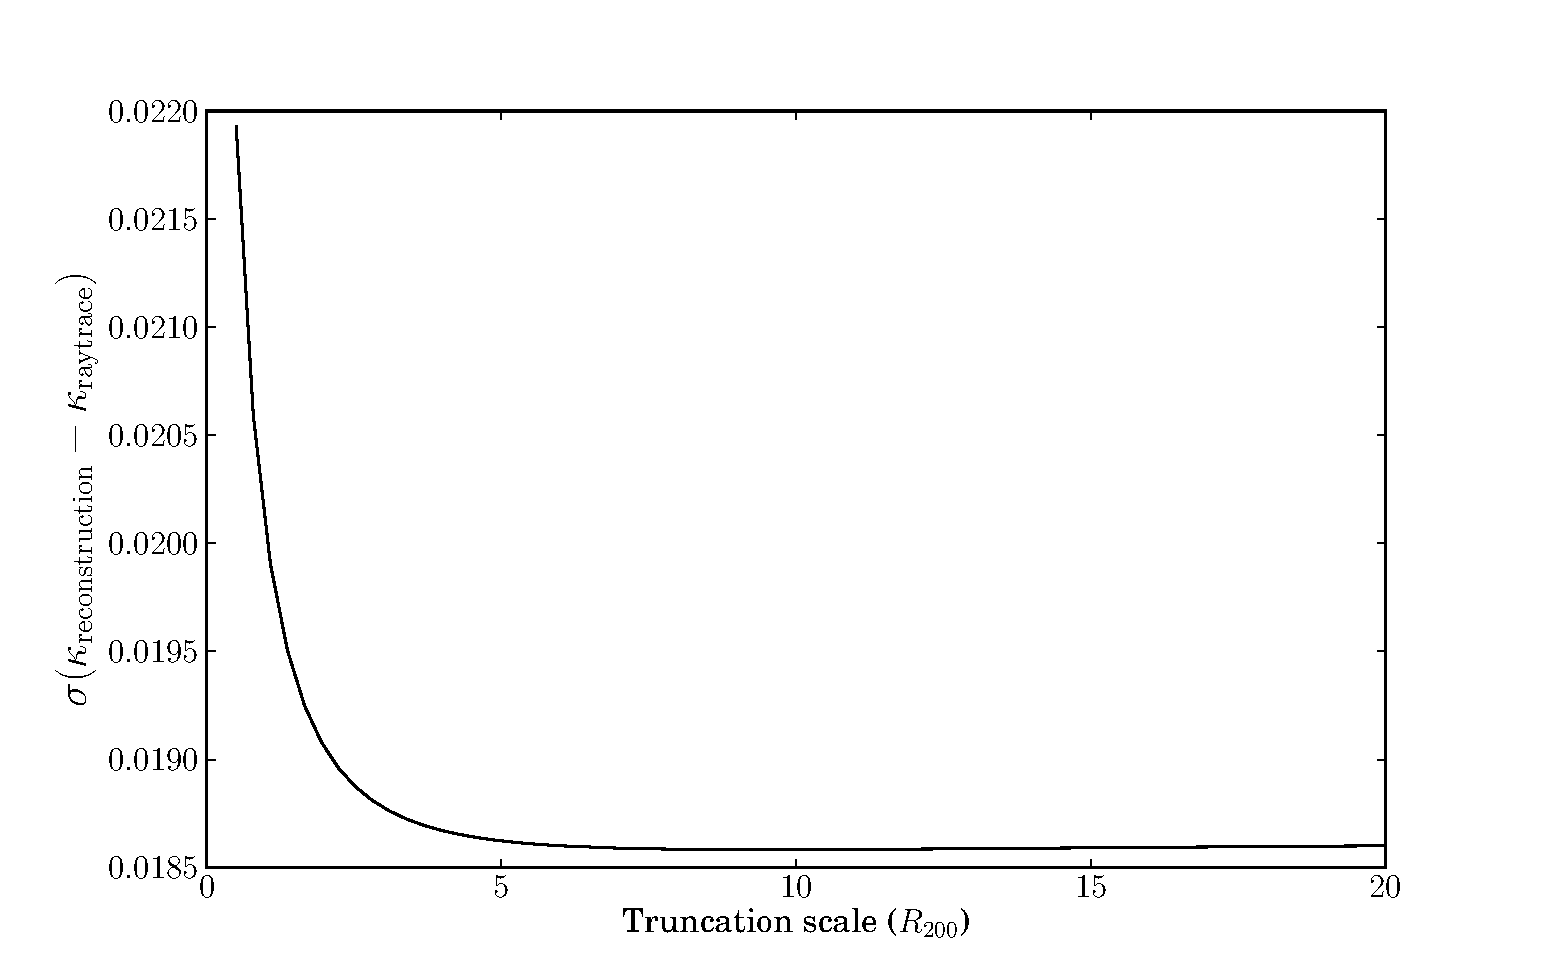
\includegraphics[width=\columnwidth]{figs/truncation_scatter.eps}
\caption[magcut]{The standard deviation in $\kapparec$ minus $\kapparay$ as a function of halo truncation radius in virial radii, using the truncated NFW profile of \citet{BMO}. In our models we truncate our halos at 5$R_{200}$}
\label{fig:ScattervsTruncation}
\end{figure}

For $\sumkappah$ to provide useful constraints on $\kapparay$, it is important that $\kapparay$ and $\sumkappah$ are as similar as possible. Figure \ref{fig:bias} shows that indeed $\sumkappah$ is a good estimator, regardless of the individual value of $\sumkappah$. At fixed $\sumkappah$ we find that the scatter in $\kapparay$ grows with $\sumkappah$; our reconstruction is better at reproducing underdense lines of sight than overdense lines of sight.

\begin{figure}
% 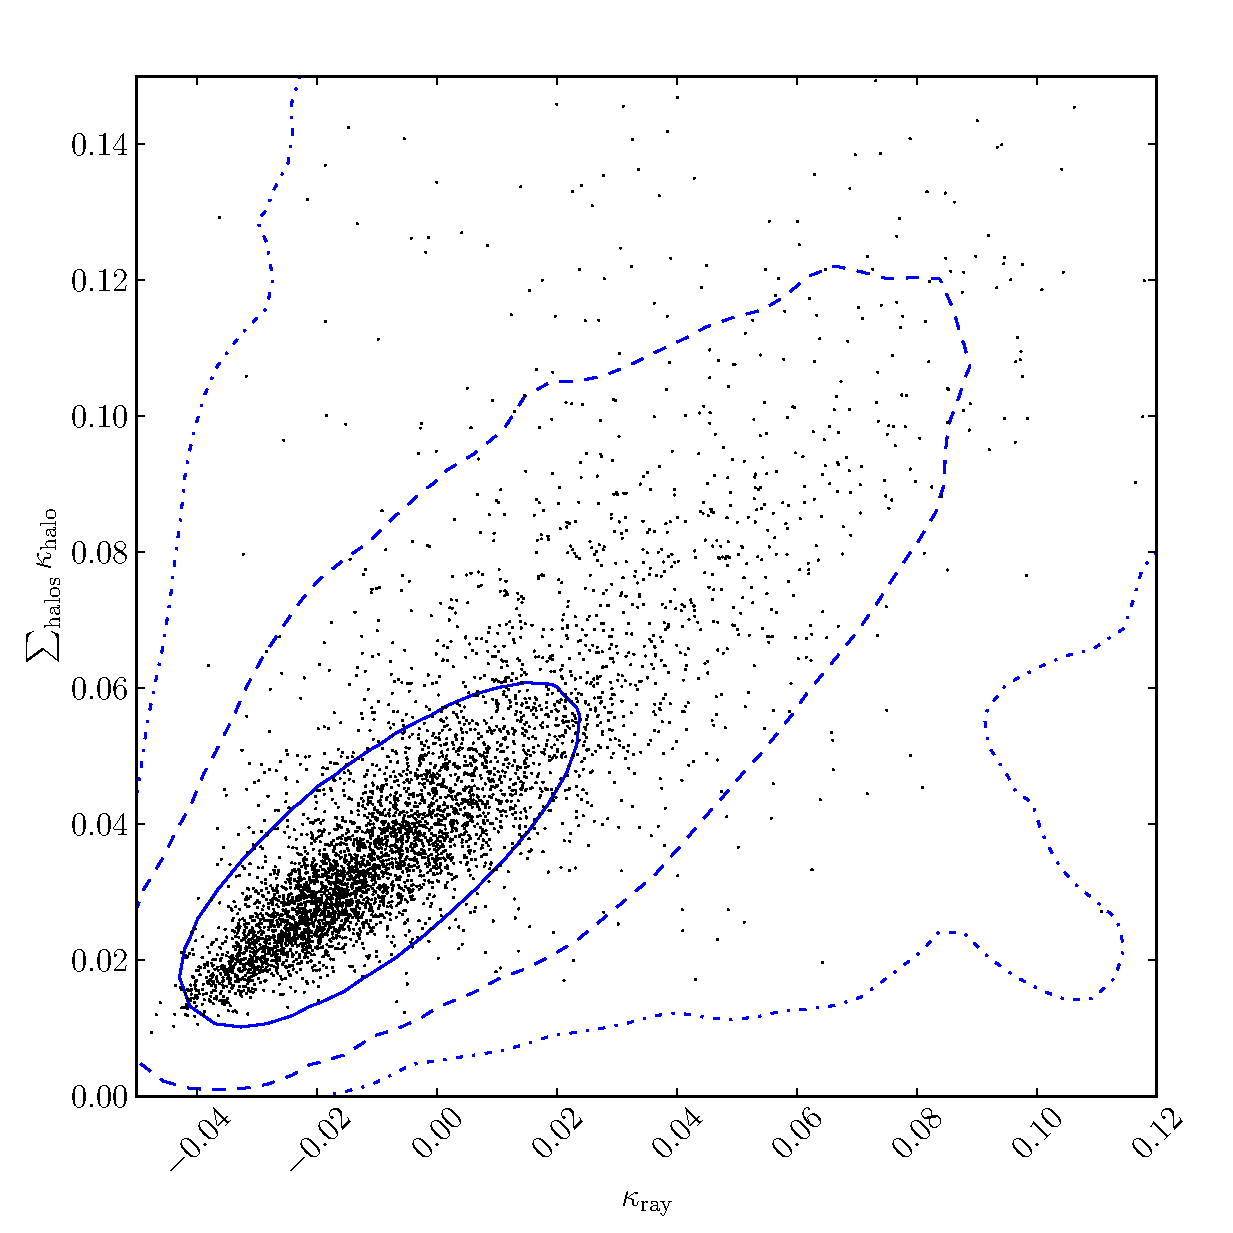
\includegraphics[width=\columnwidth]{figs/perfectc.eps}
\caption[Biased?]{$\sumkappah$ verses $\kapparay$ for 100000 reconstructed lines of sight. $\sumkappah$ traces $\kapparay$, but with a non-zero offset which is due to the negative connvergence from voids. At fixed $\sumkappah$ the scatter in $\kapparay$ grows with $\sumkappah$.}
\label{fig:isitbiased}
\end{figure}

The intrinsic error between the results of the halo based prescription and the raytraced convergence is an unavoidable error, even with perfect knowledge of halo mass and position. Before investigating the errors caused by imperfect knowledge of halo mass and redshift, we investigate the errors induced by a magnitude limited reconstruction and a field of view limited reconstruction. The halos in our catalogue are given magnitudes by the semi-analytic model of \citet{deLucia+Blaizot2007} and by applying magnitude cuts to our catalogue, we can investigate the scatter caused by unobserved halos. The majority of the convergence comes from halos with an $i$ magnitude between 18 and 24. Figure \ref{fig:magcut} shows that the width of $\kapparec-\kapparay$ decreases quickly between $i=18$ and $i=24$. Objects brighter than $i=18$ are either too rare or too close to the observer to make a significant contribution to the convergence. Objects fainter than $i=24$ are too small to be important, unless they are extremely close to the line of sight where it is likely that neglecting stellar mass and using a spherical NFW prescription are too naive to adequately reconstruct $\kappax$. It is likely that ultra-faint halos (or substructures), the uncertain contribution of voids and halos deviating from our spherical truncated NFW profile are the three major sources of the scatter in $\kapparec-\kapparay$; a deeper survey will not be sufficient to decrease the size of this scatter. Since a large number of callibration lines of sight must be reconstructed to sample $\pr(\kappav)$, it may prove unrealistic to reconstruct the calibration lines of sight out to 5 arcminutes. Figure \ref{fig:radcut} shows the width of $\kapparec-\kapparay$ as a function of reconstruction radius; in almost all cases there is no significant contribution to $\kappa$ from halos that are centred more than 1 arcminute away, although large groups or clusters can sometimes still make a contribution as far out as four arcminutes. For the rest of this work we will continue to model all of the halos out to 5 arminutes with an $i$ magnitude greater than 26, although a reconstruction with fields going out to two arcminutes and down to $i=24$ would do almost as well.

\begin{figure}
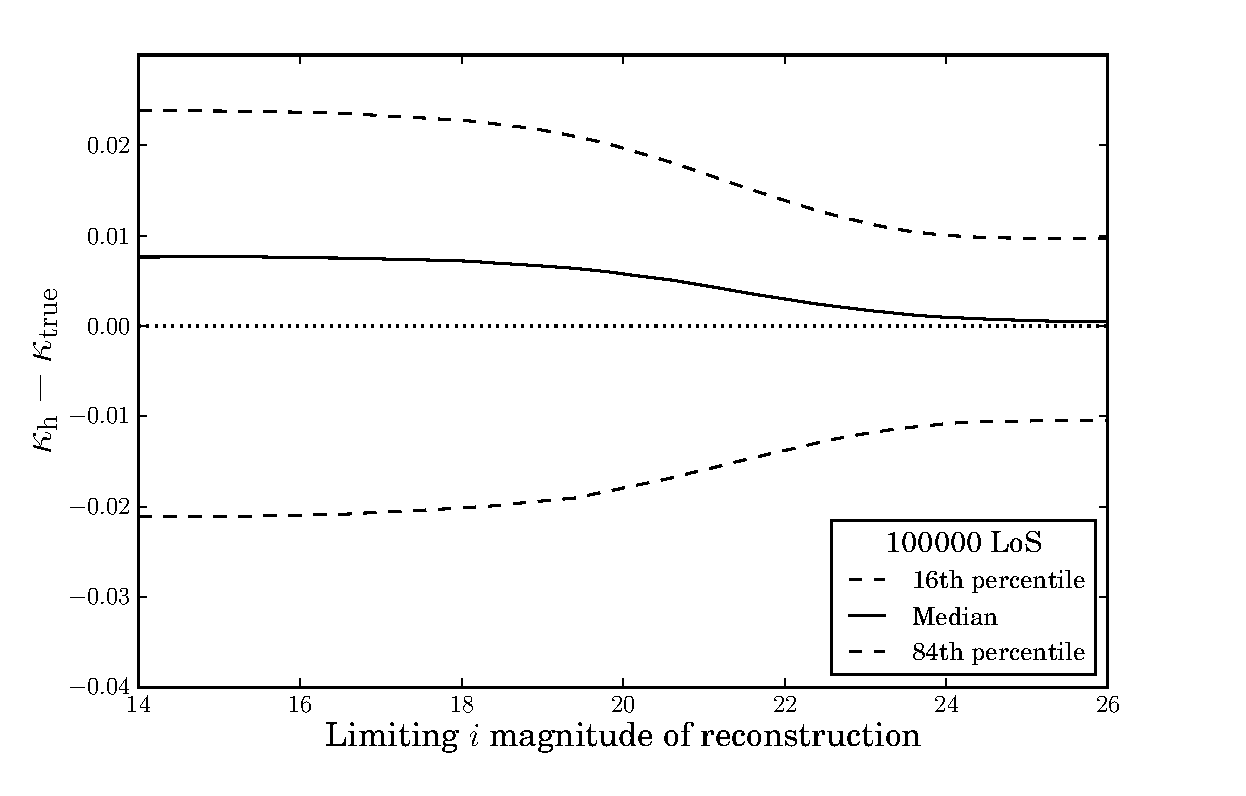
\includegraphics[width=\columnwidth]{figs/mag_scatter.eps}
\caption[magcut]{The 16, 50 and 84\% confidence intervals on $\kapparec$ minus $\kapparay$ as a function of the limiting $i$ band depth of the halo reconstruction. $\kapparec$ is given by $\sumkappah-\kappav$, where $\kappav$ is a constant such that $\left\langle\kapparec\right\rangle=0$. The majority of the constraining power comes from reconstructing halos with magnitudes between $18<i<24$}
\label{fig:magcut}
\end{figure}
\begin{figure}
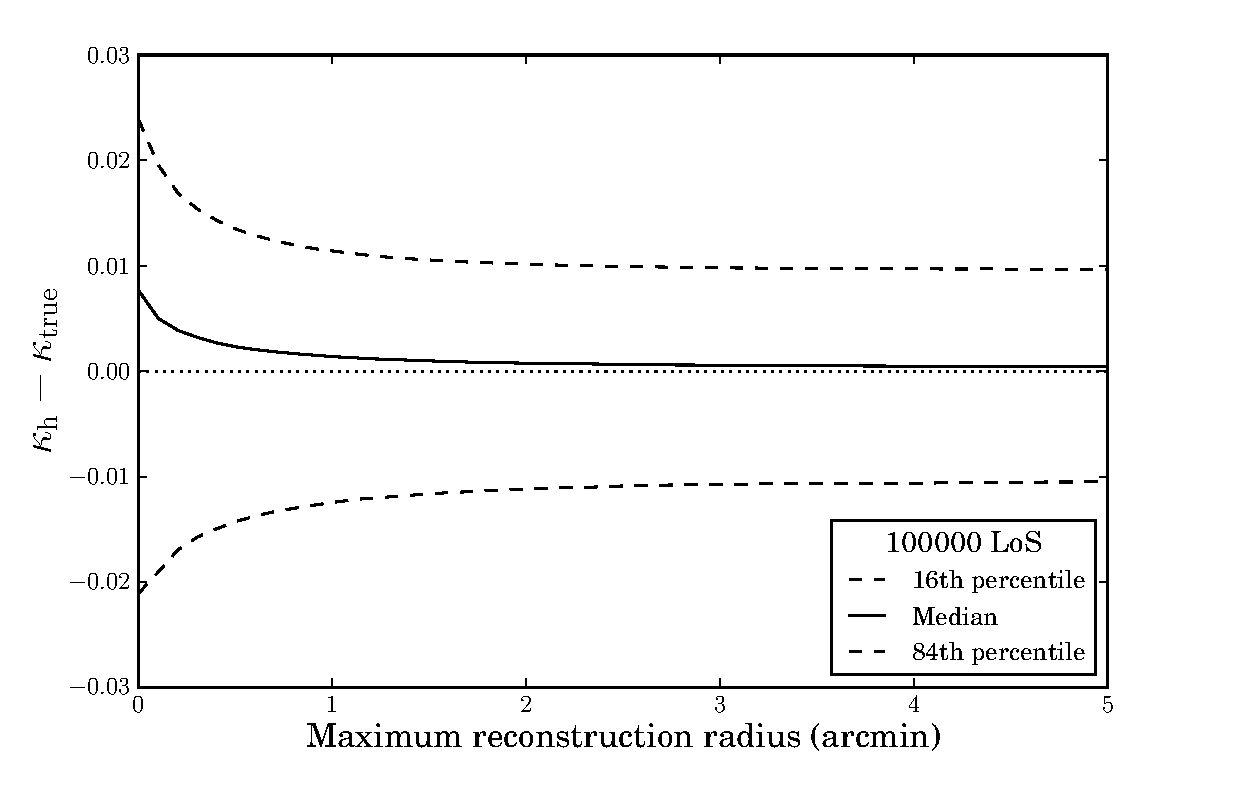
\includegraphics[width=\columnwidth]{figs/radius_scatter.eps}
\caption[radius cut]{The 16, 50 and 84\% confidence intervals on $\kapparec$ minus $\kapparay$ as a function of the limiting radius (in arcminutes) beyond which halos are not reconstructed. The majority of the convergence comes from halos centred within an arcminute of the line of sight}
\label{fig:radcut}
\end{figure}

The final test that we apply to the perfect knowledge reconstruction is to apply the marginalization outlined in Section \ref{subsec:voids}. Taking the reconstructed $\sumkappah$ for $1\times 10^{5}$ lines of sight we form the joint distribution, P$(\kapparay,\sumkappah)$ and marginalize over all sightlines with a similar $\sumkappah$ to give P($\kappax$). We define the bias as the difference between the expectation value of $\kappax$ and the known true value of $\kapparay$ for each Line of sight and we define the reconstruction width as half the width of the interval containing the central $68\%$ of the probability P($\kappax$). From $1\times 10^{4}$ reconstructed lines of sight we find the the bias to have mean of $-9.5\times 10^{-6}$ and a mean reconstruction width of 0.0132. In the case where one assumes P$(\kappax)$ is given by the global P$^{\rm global}(\kappax)$, the same $1\times 10^{5}$ lines of sight show a mean bias of $4.3\times 10^{-5}$ and mean reconstruction width of 0.237. Within the statistical error both methods are unbiased, but for any individual line of sight the bias is typically 1.8 times smaller with the reconstructed P$^{\rm reconstruction}(\kappax)$, rather than global P$^{\rm global}(\kappax)$. 

%%%%%%%%%%%%%%%%%%%%%%%%%%%%%%%%%%%%%%%%%%%%%%%%%%%%%%%%%%%%%%%%%%%%%%%%%%%%%%%%

\section{Applying the Halo Model approximation to mock catalogs}
\label{sec:obsMstar+z}

Real attempts to reconstruct the convergence along a line of sight will not have direct access to the masses of dark matter halos, 
and will likely not have access to their spectroscopic redshift either. Instead these properties must be inferred from astrophysical
observables. In principle the only observables are astrometric positions, photometric colours and possibly spectra. In this section we
quantify the errors induced by inferring the halo mass and redshift from the observables. Much work has already focused on using
photometric colours to infer stellar mass \citep[\eg][]{xxx} and redshifts \citep[\eg][]{BPZ}, in line with these we shall use
stellar mass and photometric redshifts (with appropriate errors), as the observables that must be converted into an estimate
of $\kappax$. We will investigate two main sources of error: inferring halo mass given observed stellar mass and placing halos at the wrong redshift due to photometric redshift error.

We generate a stellar mass for each halo according to the stellar mass--halo mass relation of \citet{BehrooziEtal2010}. From this stellar mass we simulate 
an observed stellar mass by drawing a sample from $\pr(\log(M_{* \mathrm {obs}})|\log(M_{* \mathrm {true}}))$ which is given by \comments{ the product of the galaxy stellar mass function (GSMF) of \citet{Fontana2006} and} a Gaussian of width $\sigma_{M_*}$ centred on $\log(M*_{\mathrm {true}})$. Where a spectroscopic redshift exists stellar masses can be estimated with typical uncertainties of 0.15 dex \citep{xxx}, however with photometric redshifts stellar mass uncertainties are typically three times as large \citep{xxx}; we use $\sigma_{M_*}=0.15$ for halos with a spectroscopic redshift and $\sigma_{M_*}=0.45$ otherwise. \comments{The \citet{Fontana2006} GSMF is given by a Schechter function with redshift evolving parameters
\be
\label{eq:GSMF}
{\dee N \over \dee M_*} \propto \left(10^{(M_*-M_0(z))}\right)^{(1+\alpha(z))} \exp \left(-10^{(M_*-M_0(z))}\right)
\ee 
where $M_0(z)=11.16+0.17z-0.07z^2$ and $\alpha(z)=-1.18-0.082z$.} For photometric redshift errors we draw a redshift from $\pr(z_{\rm true}|z_{\rm obs})$ which we take as a Gaussian of width $0.1(1+z_{\rm spec})$ centred on $z_{\rm spec}$, where $z_{\rm spec}$ is the halo's true redshift in the \MS catalogue

For each  source of error, we reconstruct 40000 calibration lines of sight and 10000 mock lens lines of sight, following the proceedure outlined in Section \ref{sec:model}. Reconstructing the lines of sight with perfect knowledge of the redshift but an uncertain stellar mass, we find that the width of $\Pr\left(\sumkappah \right)$ grows with the expectation value of $\sumkappah$; this is not surprising since the low $\sumkappah$ lines of sight are relatively empty and so there are few opportunities for uncertainties in the halo masses to propogate into $\sumkappah$ uncertainties. After applying the void correction the expected bias from our 10000 mock lenses is $6.7\times 10^{-5}$ and the mean reconstruction width is 0.0145; this is the typical reconstruction error that could be expected from a complete spectroscopic survey of the field, it is ten percent worse than the reconstruction given perfect knowledge of the halo masses and redshifts but still 1.6 times better than using the global P$^{\rm global}(\kappax)$ although a complete spetroscopic survey is still unrealistic. The distribution of the widths of $\Pr\left(\kappax \right)$ is shown in Figure \ref{fig:width1}


\begin{figure}
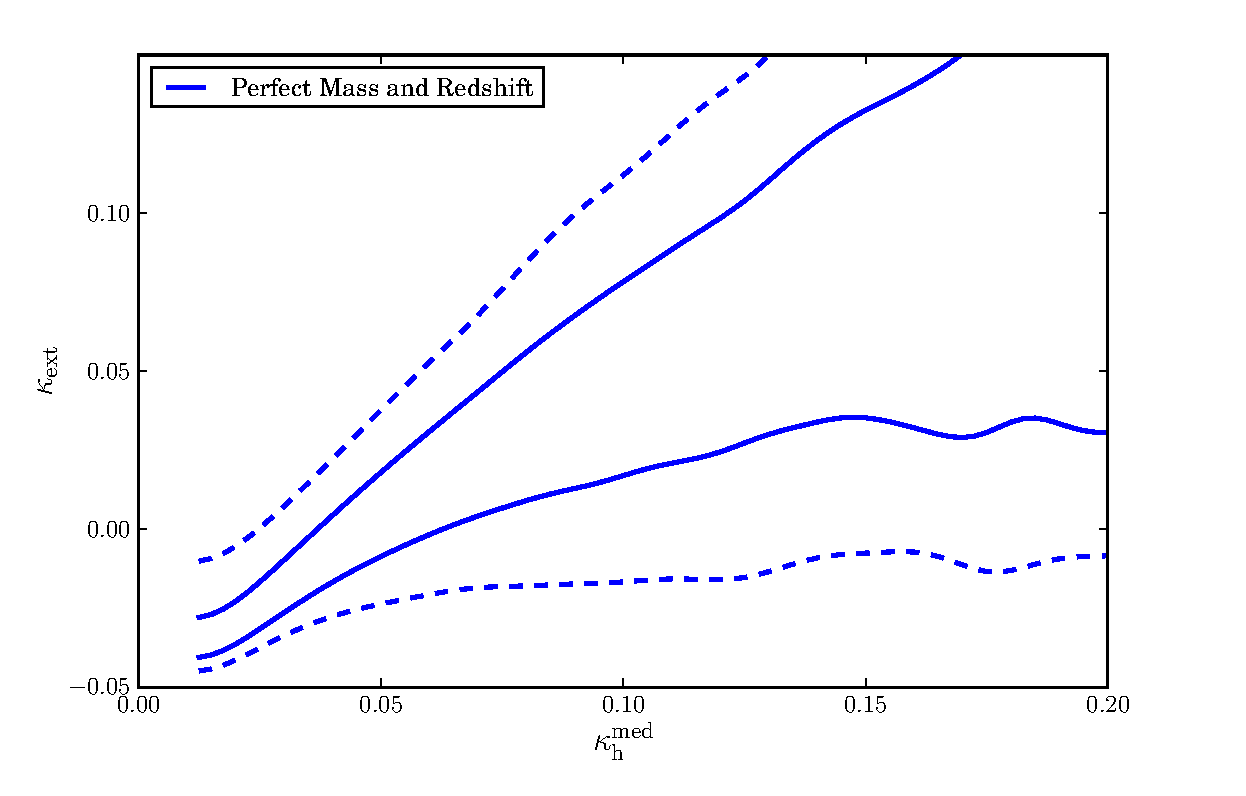
\includegraphics[width=\columnwidth]{figs/cornerplot.eps}
\caption{68 \% and 95 \% contours of the joint distribution $\pr(\kapparay, \tilde\kappa_{\rm halos})$ given a mock reconstruction of our 40000 calibration lines of sight. $\tilde\kappa_{\rm halos}$ is the median of $\pr(\sumkappah)$ given a spectroscopic redshift for each halo. $\kapparay$ and $\tilde\kappa_{\rm halos}$ are strongly correlated, despite the blurring effect of uncertain halo masses.}
\label{fig:corner}
\end{figure}

\begin{figure}
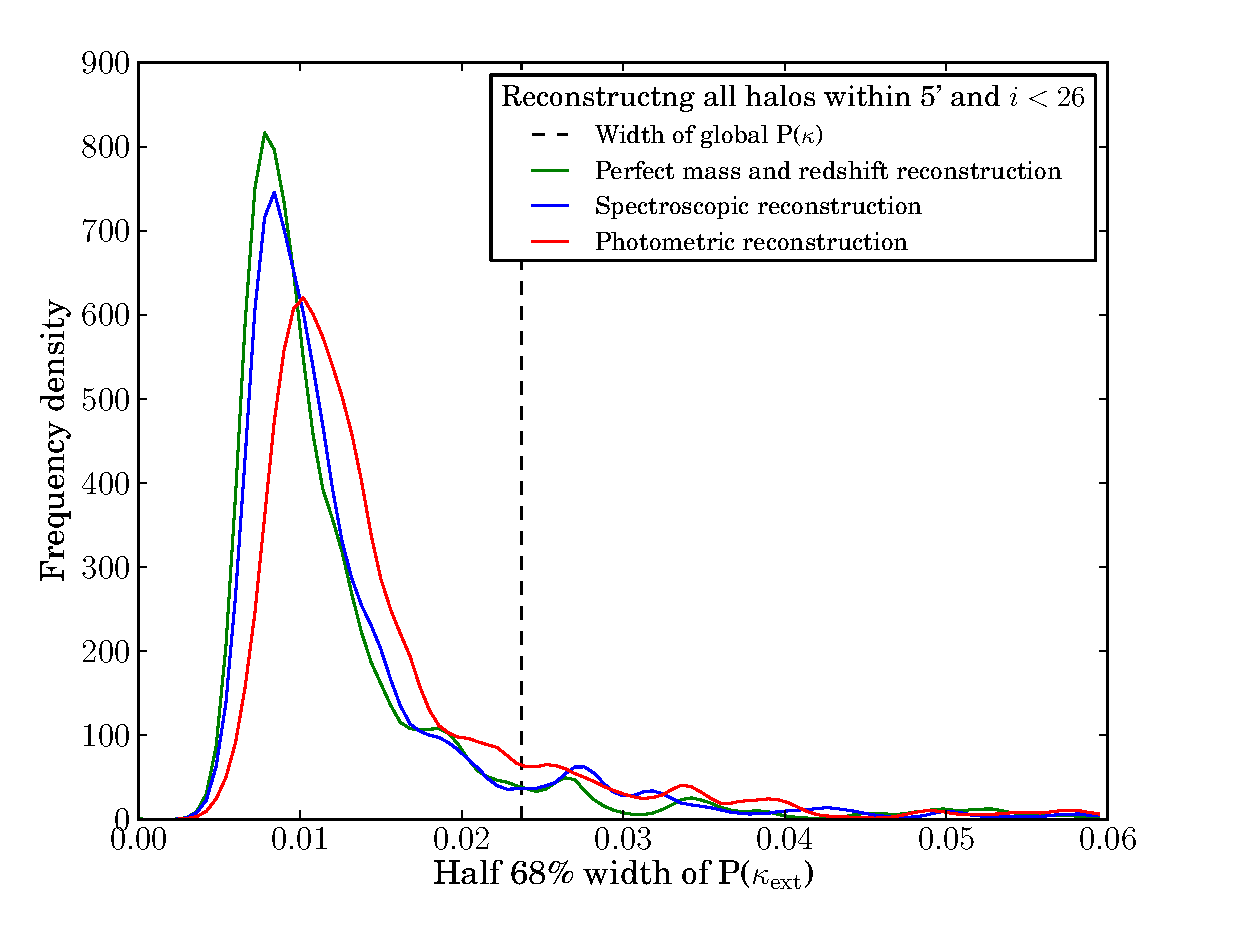
\includegraphics[width=\columnwidth]{figs/widths.eps}
\caption{Widths of $\pr(\kappax)$ after applying our reconstruction of all halos down $to i=26$ and within 5 arcminutes of the line of sight. Results for 10000 lines of sight are shown. Green is for a reconstruction given perfect knowledge of halo mass and redshift, blue is for a reconstruction given a spectroscopic redshift for every halo, and red is for a reconstruction with photometric redshifts only. The dashed black line shows the width of the global $\pr(\kappax)$ distribution; the reconstruction process provides roughly a factor of 2 improvement for the majority of lines of sight. Spectroscopic redshifts improve the reconstruction, but at signifcant observational cost.}
\label{fig:width1}
\end{figure}

Inferring the stellar mass of a galaxy from its magnitude and colours requires an estimate of how far away the galaxy is; without a spectroscopic redshift the the infered stellar mass is less precise. In principle the photometric redshift is correlated with the infered stellar mass, however we do not model this effect since the convergence from the outskirts of an individual halo is only weakly dependant on redshift at fixed mass: the redshift error is small effect on the recovered $\pr(\kappa)$ when compared to the effect of uncertain stellar masses.  With only photometric redshifts the uncertainty on $\sum\kapparec^{\rm halos}$ is much larger than the spectrocopic case, but this does not propogate into a much larger bias after applying the void correction; with a purely photometric reconstruction of the 10000 mock lightcones the results have a mean bias of $1.1\times 10^{-4}$ and a mean width of 0.0158. On average a purely photometric reconstruction of the field gives an unbiased $\pr(\kappax)$ that is 1.5 times tighter than assuming the global $\pr^{\rm global}(\kappax)$. 


%\subsection{Reconstructions of Smaller and Shallower Fields}

\begin{figure}
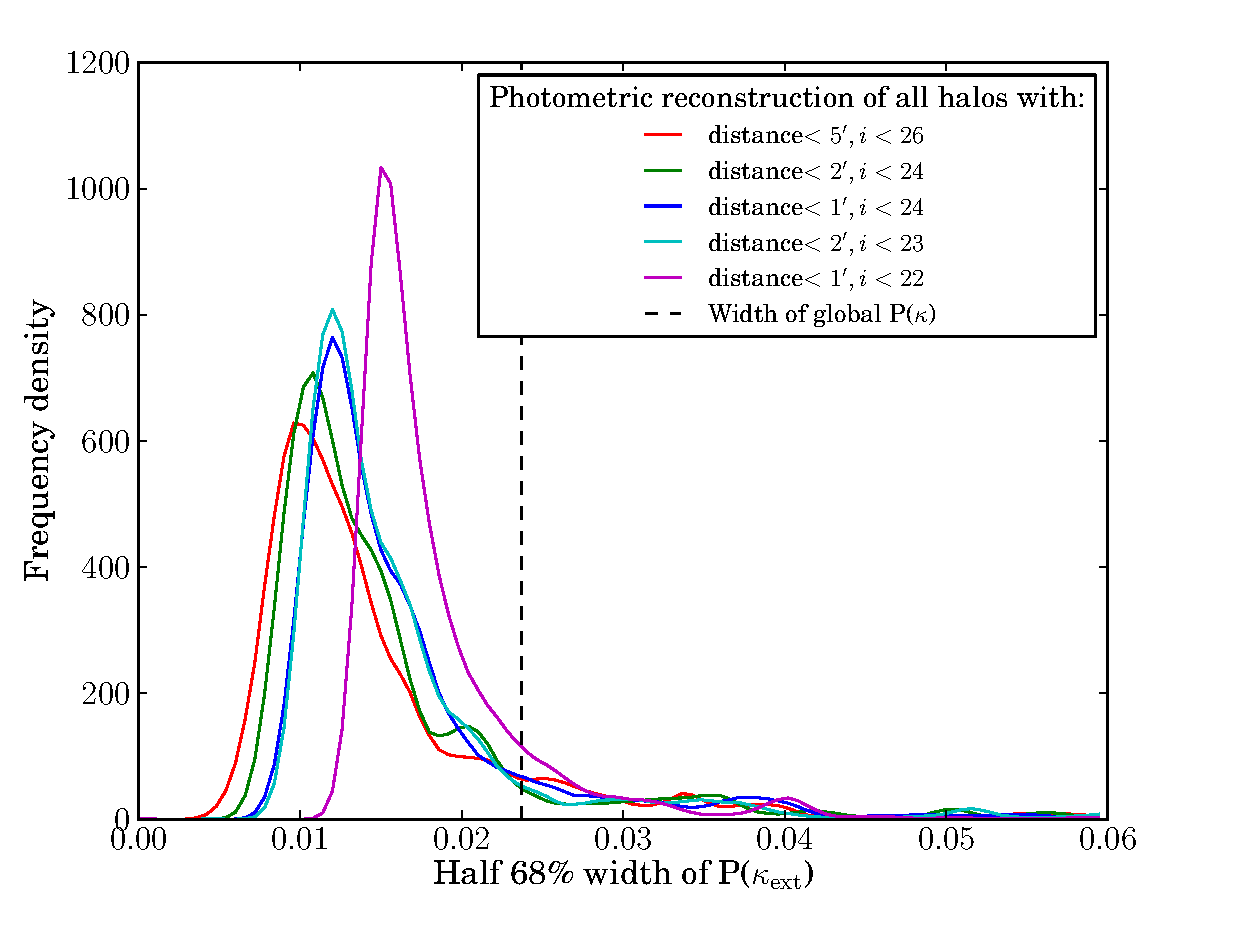
\includegraphics[width=\columnwidth]{figs/widths2.eps}
\caption{Widths of $\pr(\kappax)$ after a photometric reconstruction of all halos within different fields. The different field sizes and depths are given in the legend. As the field becomes smaller or shallower, fewer halos are being reconstructed and so the width of $\pr(\kappax)$ grows.}
\label{fig:width2}
\end{figure}


Reconstructions of real lines of sight may not have access to the deep, large calibration fields that we have used upto this point. We can perform the same reconstruction but for a more modest mock survey. Given the results of Section \ref{sec:knownMh+z} we predicted that a reconstruction of the field out to 2 arcminutes and a magnitude limit of $i$=24 would provide similar constraints to a reconstruction going out to 5 arcminutes and going down to $i$=26. We find the mean reconstruction width to be 0.0163 for a photometric reconstruction of all the halos within 2 arcminutes that have $i<24$, this is only marginally worse than 0.0158 which was the typical width after the deeper and wider reconstruction of the previous section. The reconstruction widths for our 10000 mock lens lines of sight are shown in Figure \ref{fig:widths2}. If only photometry for halos with $i<24$ and within 1 arcminute of the line of sight is availble then the typical width of the reconstructed $\pr(\kappax)$ is 0.173. Whilst a complete spectroscopic survey of a large field would be unlikely, a hybrid strategy of obtaining spectra for a subset of objects may be feasible. Photometric redshifts are sufficient to asertain the halos which are likely to contribute most of the convergence on any given line of sight, and on average there are only $\sim 6 \pm 6$ halos per line of sight that individually contribute more than 0.002 to $\sumkappah$. We investigate a hybrid strategy of obtaining spectroscopic redshifts for all of the $i<24$ halos which contribute an individual $\kappa$ of at least 0.002 combined with a photometric redshift for all other $i<24$ halos within 2 arcminutes. For the hybrid strategy the typical width of the reconstructed $\pr(\kappax)$ is 0.0151. The observational cost of obtaining spectroscopic redshifts for several 24th magnitude galaxies may make the hybrid strategy unlikley, but obtaining photometry of a 4$\times$4 arcminute patch of sky down to $i=24$ is fast with modern telescopes. The mean reconstruction width for a photometric reconstruction of all the halos within 2 arcminutes that have $i<24$ represents an improvement of 1.5 over using the global $\pr(\kappax)$ and should be achievable at minimal observational cost.


%%%%%%%%%%%%%%%%%%%%%%%%%%%%%%%%%%%%%%%%%%%%%%%%%%%%%%%%%%%%%%%%%%%%%%%%%%%%%%


\section{Testing for Systematic errors}
\subsection{Using the wrong M$_{\rm halo}$-M$_{*}$ relation}
\subsection{Selecting bias from a subset of lines of sight?}
\subsubsection{Selecting only the lines of sight with tight $\pr(\kappax)$}
\subsubsection{Selecting only high shear lines of sight}

%%%%%%%%%%%%%%%%%%%%%%%%%%%%%%%%%%%%%%%%%%%%%%%%%%%%%%%%%%%%%%%%%%%%%%%%%%%%%%
\comments{

\subsection{Comparison with Other Treatments of $\kappax$}
\label{sec:Dt:selection} 

\phil{How does distance accuracy compare with simple averaging? eg assuming
$\kappax = 0$ for all lenses. How does it compare with the no data situation?
eg where the intrinsic distribution of kappa is used as $Pr(\kappax)$.}

What is the expected bias and scatter (centroid position and width) of P(D) as a
function of N lenses? How does reconstruction compare with P(D) derived using
P(kappa|N45) for each lightcone? How does reconstruction compare with P(D)
derived assuming kappa=0 for each lightcone?

Also: compare with simple averaging. This will fail if lenses are selected to
live on over-dense lines of sight. Stefan's plot in Suyu et al shows effect of
selection - what is the resulting bias? Few percent? This is the target to beat,
need to find it out.

\subsection{Improving the Accuracy with More Information}
\label{sec:Dt:selection} 

\phil{How does distance accuracy improve with:}
\begin{itemize}
\item Spectroscopic coverage? For galaxies above some mlim? For targets with
high kappa contribution (based on photometry)?
\item IR coverage for all objects? Improves photo-z and Mstar.
\item Including shear information from lens model? Assume accurate but
uncertain extertanl shear.
\end{itemize}
}
%%%%%%%%%%%%%%%%%%%%%%%%%%%%%%%%%%%%%%%%%%%%%%%%%%%%%%%%%%%%%%%%%%%%%%%%%%%%%%

\section{Discussion}
\label{sec:discuss}

We have shown that reconstructing the matter due to halos along any line of sight can give meaningful and unbiased constraints on the external convergence along that line of sight. The total convergence along a line of sight is strongly correlated with the reconstructed $\sumkappah$. However since our model ignores voids and assumes all halos follow a spherical truncated-NFW profile our model does not include all of the relevant physics, hence the width of our resulting $\pr(\kappax)$ is still typically $\sim$0.01, even with a perfect knowledge of every halo's virial mass and redshift. To make further progress a more advanced treatment of both voids and halos will be necessary. Interestingly, we have found that the most empty lines of sight can be reconstructed with the most precision. $\kappax$ for empty lines of sight have little contributions from halos and a large contribution from voids; since they have the tightest PDFs after the reconstruction it seems that our model's biggest uncertainties are driven by naively reconstructing halos rather than neglecting voids. With a photometric reconstruction of the field there is only a small broadening compared to the perfect knowledge reconstruction; it seems that deviations from sphericity and dark matter clumping within the main halo are the dominant uncertainies rather than uncertainties in the halo mass. Inferring halo ellipticity and dark matter clumping will likely always remain a difficulty for line of sight reconstruction; as Figures \ref{fig:magcut} and \ref{fig:width2} show observing deeper than 24th magnitude does not signifcantly help the reconstruction. Because our reconstruction is mostly limited by the model, spectroscopic coverage can only provide a modest improvement to the reconstruction and at significant observational cost.

For a small fraction of lines of sight, $\pr(\kappax)$ remains very broad even after applying our reconstruction; these lines of sight are typically the most overdense lines of sight in the universe. For time-delay cosmography the most observationally expensive task is the lightcurve monitoring, whilst making photometric observations of a 4$\times$4 arcminute patch of sky survey down to 24th magnitude is a relatively cheap. We have shown that with a single epoch observation of the region around a strong lens it is possible to infer $\pr(\kappax)$. If a line of sight has a broad $\pr(\kappax)$ it can be rejected {\it before} the investment of longterm lightcurve monitoring.

The method we have outlined can also be used to estimate the external shear
along a line of sight. Shear is an observable that can be extracted from
strong lens modelling, however there is a degeneracy between internal and
external shear. Progress has been made in disentangelling external and
internal shear \citep[\eg][]{xxx} but there are still significant
uncertainties: \citet{WongEtal2011} attempted to match the shear from strong
lens models with a reconstruction of the local lens group environment, but
found a tension between the strong lens model and the reconstruction of the
environment. Since \citet{WongEtal2011} only reconstructed the local lens
group, rather than the full line of sight contribution, it is unclear whether
the external shear from lens models can be reconciled with a line of sight
reconstruction. {\it If} external shear can be measured, it provides an
additional constraint on which of the Millenium Simulation lines of sight are
similar to the reconstructed line of sight. \citet{SuyuEtal2012} found that
for RXJ1131 combining shear constriants with galaxy number count overdensity,
gave a significantly different $\pr(\kappax|\gamma,N_{45})$ copmpared to the
PDFfrom number count overdensity alone, $\pr(\kappax|N_{45})$. 



%%%%%%%%%%%%%%%%%%%%%%%%%%%%%%%%%%%%%%%%%%%%%%%%%%%%%%%%%%%%%%%%%%%%%%%%%%%%%%

\section{Conclusions}
\label{sec:conclude}

In this work we have investigated a simple halo model prescription for
reconstructing all the mass along a line of sight to an intermediate redshift
source. We have used the ray-traced lensing convergence along lines of sight
through the Millenium Simulation to test this approach, and to calibrate
estimates of the total convergence along a line of sight to an observed
distant galaxy made by summing the convergences due to each object in a
photometric catalogue. Having found that the reconstruction process is effective given perfect
knowledge of halo mass and redshift, we investigated the effects of reasonable
uncertainties in the stellar mass and redshift of each halo, and propogated
these uncertainties into a $\pr\left(\sumkappah\right)$ for each line of
sight. We draw the following conclusions:

\begin{itemize} 

\item Our model uses a truncated spherical NFW profile for
each dark matter halo and neglects voids, but despite the model's simplicity
the reconstructed $\sumkappah$ is a good tracer of $\kappax$.  We found that
with perfect knowledge of the halo mass and redshift (from the Millenium
Simulation catalogs), the reconstruction gives an unbiased estimate of
$\pr(\kappax)$ for a single line of sight that is almost almost a factor of 2
less broad than the global $\pr(\kappax)$. 

\item  For the most overdense lines of sight, the reconstruction produces a
very broad PDF, but since the reconstruction can be performed before follow-up
time is invested it will be possible to discard the most uncertain lines of
sight and prevent the waste of follow-up time. 

\item With complete spectroscopic redshift coverage and just an empirical
stellar mass to halo mass relation, we find that the median of
$\pr\left(\sumkappah\right)$ is a useful indicator for generating an estimate
of $\pr(\kappax)$ from the ensemble of simulated lines of sight. The resulting
PDF tends to be around 10\% broader than it would have been given perfect
knowledge of both halo mass and redshift; given only photometric redshifts
(which in turn give rise to much less certain stellar masss estimates) causes
another $\sim$10\% increase to the width of $\pr(\kappax)$.

\item It is very rare for halos further than 2 arcminutes to make a
significant contribution to $\kappax$. We also found that including halos
whose host galaxy is less luminous than $i=24$ does not significantly improve
our reconstruction proceedure. A photometric survey to this depth of a
4$\times$4 arcminute patch around the lens would approach the limiting
uncertainties of our simple reconstruction recipe, and yield a 
$\pr(\kappax)$ that has, on average, a width of 0.0163 --
50\% less broad than the global $\pr(\kappax)$.

\item We find that the lines of sight with the sharpest $\pr(\kappax)$ are
typically under-dense. With a photometric reconstruction of all lens fields,
and following up only the lenses with the most constraining $\pr(\kappax)$,
the width of the dominant statistical uncertainty in time-delay cosmography
can be halved, whilst at the same time decreasing any potentail for a
systematic error due to lenses being biased in $\kappax$.

\end{itemize}

\todo{Tom}{Add more conclusions about bias in a large sample of lenses...}

\todo{Tom}{Wrap up}


%Our conclusions can be summarised as follows:
%\begin{itemize}
%\item With perfect 
%\item And we found this too.
%\end{itemize}

% \item Faint galaxies and other dark structures will not appear in a photometric
% object catalog, but they will contribute convergence at some level. How much of
% the total external convergence in a time delay lens system comes from visible
% galaxies? How does this change as a function of magnitude cut? 

% \item Can the true (ray-traced) convergence be recovered by halo model
% reconstruction, and with what scatter and residual bias? Which aspects of the 
% model dominate these uncertainties?

% \item When faced with a newly-detected lens, surrounded by galaxies on the sky,
% we have some choices to make when planning follow-up observations.
% Which are the most important galaxies, with regard to the external convergence
% produced? Can nearby groups and clusters be straightforwardly accounted for? If
% lenses with such massive structures nearby are discarded, what impact does that
% have on the distance accuracy?



%%%%%%%%%%%%%%%%%%%%%%%%%%%%%%%%%%%%%%%%%%%%%%%%%%%%%%%%%%%%%%%%%%%%%%%%
%%  ACKNOWLEDGMENTS
%%%%%%%%%%%%%%%%%%%%%%%%%%%%%%%%%%%%%%%%%%%%%%%%%%%%%%%%%%%%%%%%%%%%%%%%

\section*{Acknowledgments}
 
TC thanks Vasily Belokurov for guidance and discussions.
We thank Risa Wechsler and Peter Behroozi for useful discussions and 
suggestions.
\input{acknowledgments.tex}

%%%%%%%%%%%%%%%%%%%%%%%%%%%%%%%%%%%%%%%%%%%%%%%%%%%%%%%%%%%%%%%%%%%%%%%%%%%%%%
%  APPENDICES
%%%%%%%%%%%%%%%%%%%%%%%%%%%%%%%%%%%%%%%%%%%%%%%%%%%%%%%%%%%%%%%%%%%%%%%%%%%%%%

\appendix

%%%%%%%%%%%%%%%%%%%%%%%%%%%%%%%%%%%%%%%%%%%%%%%%%%%%%%%%%%%%%%%%%%%%%%%%%%%%%%

\section{Truncated NFW halos}
\label{appendix:halos}

 Defining $x$ as the dimensionless projected radial distance $R/r_{s}$ and $\tau$ as the dimensionless truncation radius $r_{t}/r_{s}$, \citet{BMO} derives the projected mass density, which is given by:
\begin{align}\label{eq:kappaBMO}
\Sigma_{\rm}(x) = {2\tau^2 \over (\tau^2+1)^2}\left(
        {\tau^2+1\over x^2-1}\left(1-\mathcal{F}(x)\right)
        +
        2\mathcal{F}(x)\right.\nonumber\\
        -
        \left. {\pi \over \sqrt{\tau^2+x^2}}
        +
        {(\tau^2-1)\mathcal{L}(x,\tau)
        \over
        \tau\sqrt{\tau^2+x^2}}\right)
\end{align}
where $\mathcal{F}(x)$ and $\mathcal{L}(x,\tau)$ are defined as
\be\label{eq:F} 
\mathcal{F}(x) \equiv \begin{cases}  \frac{{\rm cos}^{-1} (1/x)}{\sqrt{x^2-1}} \hspace{0.2cm} & (x>1) \\
\\
\frac{4-x^2}{3}  & (x=1)\\
\\
\frac{ {\rm cosh}^{-1} (1/x)}{\sqrt{1-x^2}} & (x<1)
\end{cases}
\ee
\be\label{eq:L}
\mathcal{L}(x,\tau) = \ln\left(\frac{x}{\sqrt{\tau^2+x^2}+\tau}\right)
\ee
%the convergence is given by $\Sigma_{\rm BMO}(x) / \Sigma_{\rm cr}(z)$.



%%%%%%%%%%%%%%%%%%%%%%%%%%%%%%%%%%%%%%%%%%%%%%%%%%%%%%%%%%%%%%%%%%%%%%%%%%%%%%

\section{Inferring $\Mhalo$ given a noisy measurement of $\Mstarobs$}
\label{appendix:MSMH}

Given a noisy estimate of the stellar mass $\Mstarobs$ of a galaxy at redshift
$z$, how can we infer the galaxy's halo mass? We then seek the posterior
PDF $\Pr(\Mhalo|\Mstarobs)$, which can be expanded as follows:

\begin{eqnarray}
&& \Pr(\Mhalo|\Mstarobs,z) = \notag\\
&& \int d\Mstar \Pr(\Mhalo|\Mstar,z) \Pr(\Mstar|\Mstarobs,z), \notag\\
&\propto& \int d\Mstar \Pr(\Mstarobs|\Mstar) \Pr(\Mstar|\Mhalo,z) \Pr(\Mhalo|z),
\label{eq:mhalo-mstar}
\end{eqnarray}
where we have used Bayes' Theorem twice to replace
$\Pr(\Mhalo|\Mstar,z) \Pr(\Mstar|z)$ with 
$\Pr(\Mstar|\Mhalo,z) \Pr(\Mhalo|z)$, and 
to invert $\Pr(\Mstar|\Mstarobs)$ into the sampling
distribution $\Pr(\Mstar|\Mstarobs)$, which we recognise as the likelihood
function for the observed stellar mass. Note that the ``true'' $\Mstar$ of the
galaxy is marginalised out: we are only interested in reconstructing the halo
mass. The last two terms in
\eqref{eq:mhalo-mstar} are the $\Mstar-\Mhalo$ relation from
\citet{BehrooziEtal2010}, and the halo mass function $\Pr(\Mhalo|z)$, at the
given redshift. We can
tabulate the product of these two from our Millenium Simulation catalog,
constructing a two-dimensional histogram of halo masses and their associated
true stellar masses (drawn from the Behroozi relation). 

For each galaxy, we compute the likelihood function for its $\Mstarobs$ as a
function of the unknown $\Mstar$, and multiply it by our tabulated joint PDF.
This heavily downweights halos with $\Mstar$ values outside the observed
range. We then do the marginalisation integral by Monte Carlo, drawing
(two-dimensional) sample parameter vectors
from the downweighted histogram, discarding the $\Mstar$ values, and
constructing a one-dimensional histogram that is an estimate of
$\Pr(\Mhalo|\Mstarobs)$.

\todo{Matt}{Edit the above text to add a note on how we do the sampling in
practice, via the CDF.}

If the redshift of the galaxy is uncertain, we need to take this uncertainty
into account; for example, for each sample drawn from the photometric redshift
posterior PDF $\Pr(z|{\rm colors})$, we can draw a sample $\Mhalo$ using the
above procedure.


%%%%%%%%%%%%%%%%%%%%%%%%%%%%%%%%%%%%%%%%%%%%%%%%%%%%%%%%%%%%%%%%%%%%%%%%%%%%%%

\section{Accounting for uncatalogued low mass halos, and voids}
\label{appendix:smooth}

Our halo model allows us to infer a halo mass $\Mhalo$ for each galaxy in a
photometric catalog; under the weak lensing approximation described in
\Sref{sec:theory} we can compute the contribution of each of these halos to
the overall convergence and shear amplitude, assuming a homogeneous
Friedman-Robertson-Walker metric and the concordance $\Lambda$CDM cosmological
parameters for the angular diameter distances to calculate the critical
density for each lens plane. Clearly this approach will tend to over-estimate
the convergence, since we are placing massive halos into a volume that has
already been assumed to be full of homogeneously distributed matter with the 
mean cosmological density. In practice, the space between massive halos will
contain a) low mass halos that are not bright enough to be detected and b)
empty space where the density is below that of the mean. A rigorous treatment
of this complex situation is beyond the scope of this paper, but is being
investigated (Blandford et al, in preparation). In this appendix we describe
our empirical approach to accounting for the missing mass and voids. 

Let the summed convergence due to halos in our galaxy catalog be $\kappah$.
Given some assumptions about halo density profile and shape, this parameter
can be inferred from a set of uncertain halo mass estimates (which have in
turn been inferred from noisy measurements of galaxy redshift and stellar mass
as described in \Aref{appendix:MSMH}). We assume each halo to be a
spherically-symmetric NFW profile, and neglect the contribution of the stellar
mass to the convergence. The halo mass inference for the $k^{\rm th}$ galaxy 
is stored as a list of sample values of $\Mhalok$ drawn from the posterior PDF
$\Pr(\Mhalok|\Mstarobsk,z_k)$; computing the contribution to the convergence
due to this halo at the target line of sight for each sample gives, in turn, 
a set of
samples drawn from the PDF $\Pr(\kappahk|\Mstarobsk,z_k)$. We then generate
samples from $\Pr(\kappah|\{\Mstarobsk,z_k\})$ by drawing a sample $\kappahk$
for each halo, summing over halos to get $\kappah$, discarding those
samples and moving down the lists.

The PDF $\Pr(\kappah|\{\Mstarobsk,z_k\})$ will, in general, be broad (due to
the uncertainties involved in halo mass estimation). It will also be shifted
towards high values of convergence, due to the FRW approximation described
above. What we really want is an inference of $\Pr(\kappa|\{\Mstarobsk,z_k\})$
instead. We can obtain this by considering the expansion:
\begin{equation}
\Pr(\kappa|\{\Mstarobsk,z_k\}) = \int d\kappah 
   \Pr(\kappa|\kappah) \Pr(\kappah|\{\Mstarobsk,z_k\})
\label{eq:kappaconv}   
\end{equation}
The first term in the integrand relates the summed  convergence due to model
halos, $\kappah$, to the true summed convergence, $\kappa$.  In the Millenium
Simulation catalogs, we can compute a single value of $\kappah$ for each
selected line of sight from the true halo mass and redshift (and our same
assumptions of halo profile and shape), and tabulate the two-dimensional PDF
$\Pr(\kappa|\kappah)$ as a sequence of one-dimensional PDFs for $\kappa$ in a
bin at fixed $\kappah$. Note that this PDF captures the ``intrinsic scatter''
of $\kappah$ due to our assumptions about the clumpiness of mass in the
Universe; the integral combines these uncertainties with those
arising from the measurement of $\Mstarobs$ and~$z$.

For any given observed catalog then, we infer
$\Pr(\kappah|\{\Mstarobsk,z_k\})$ as described above, and then
multiply it by $\Pr(\kappa|\kappah)$; we
again do the marginalisation over $\kappah$ by Monte Carlo, drawing samples
from the two-dimensional grid and keeping only the $\kappa$ values, to form
our final result, $\Pr(\kappa|\{\Mstarobsk,z_k\})$. 
This PDF will describe, by construction, an accurate (i.e., unbiased)
measurement of $\kappa$ in the case where the Millenium Simulation halo
catalog and Behroozi et al $\Mstar-\Mhalo$ relation are themselves accurate
descriptions of galaxies and their distribution. In \Sref{sec:tests} we
investigate the amplitude of the systematic errors incurred if these
assumptions are not valid.

\todo{Matt}{Add text describing whatever sampling shortcut you derive! :-)}

% Finally, we note that \Eref{eq:kappaconv} and the method for evaluating the
% integral in it can be generalized to yield 
% $\Pr(\kappa,|\gamma||\{\Mstarobsk,z_k\})$, where $|\gamma|$ is the amplitude
% of the complex shear. The amplitude of the shear due to halos, $|\gammah|$ is
% needed in this calculation, and marginalised over -- $\gammah$ is computed by
% simple summation of its components, as in \Sref{sec:theory}. In
% \Sref{sec:includinggamma} we explore the impact that knowing $\gamma$ (from,
% for example, a strong lens model)  has on the inference of $kappa$, and how
% severe the systematic errors from getting this wrong might be.


%%%%%%%%%%%%%%%%%%%%%%%%%%%%%%%%%%%%%%%%%%%%%%%%%%%%%%%%%%%%%%%%%%%%%%%%%%%%%%
%  REFERENCES
%%%%%%%%%%%%%%%%%%%%%%%%%%%%%%%%%%%%%%%%%%%%%%%%%%%%%%%%%%%%%%%%%%%%%%%%%%%%%%

% MNRAS does not use bibtex, input .bbl file instead. 
% Generate this in the makefile using bubble script in scriptutils:

% bubble -f paper-lcr.tex references.bib 
% \input{paper-lcr.bbl}

% \bibliographystyle{apj}
% \bibliography{references}

\input{references.tex}

%%%%%%%%%%%%%%%%%%%%%%%%%%%%%%%%%%%%%%%%%%%%%%%%%%%%%%%%%%%%%%%%%%%%%%%%%%%%%%

\label{lastpage}
\bsp

\end{document}

%%%%%%%%%%%%%%%%%%%%%%%%%%%%%%%%%%%%%%%%%%%%%%%%%%%%%%%%%%%%%%%%%%%%%%%%%%%%%%


% \bibliographystyle{apj}
% \bibliography{references}

\begin{thebibliography}{99}



\bibitem[\protect\citeauthoryear{Auger et al.}{2009}]{Auger++2009} 
Auger M.~W., Treu T., Bolton A.~S., Gavazzi R., Koopmans L.~V.~E., Marshall 
P.~J., Bundy K., Moustakas L.~A., 2009, ApJ, 705, 1099 


\bibitem[\protect\citeauthoryear{Auger et al.}{2010}]{Auger++2010} 
Auger M.~W., Treu T., Bolton A.~S., Gavazzi R., Koopmans L.~V.~E., Marshall 
P.~J., Moustakas L.~A., Burles S., 2010, ApJ, 724, 511 


\bibitem[\protect\citeauthoryear{Baltz, Marshall, 
\& Oguri}{2009}]{BMO} Baltz E.~A., Marshall P., Oguri M., 2009, JCAP, 1, 15 


\bibitem[\protect\citeauthoryear{Behroozi, Conroy, 
\& Wechsler}{2010}]{Behroozi++2009} Behroozi P.~S., Conroy C., Wechsler R.~H., 2010, ApJ, 717, 379 


\bibitem[\protect\citeauthoryear{Ben{\'{\i}}tez}{2000}]{BPZ} Ben{\'{\i}}tez N., 2000, ApJ, 536, 571 


\bibitem[\protect\citeauthoryear{Collett et 
al.}{2012}]{Collett++2012a} Collett T.~E., Auger M.~W., Belokurov V., 
Marshall P.~J., Hall A.~C., 2012, MNRAS, 424, 2864 


\bibitem[\protect\citeauthoryear{De Lucia 
\& Blaizot}{2007}]{deLucia+Blaizot2007} De Lucia G., Blaizot J., 2007, MNRAS, 375, 2 


\bibitem[\protect\citeauthoryear{Falco, Gorenstein, 
\& Shapiro}{1985}]{Falco++1985} Falco E.~E., Gorenstein M.~V., Shapiro I.~I., 1985, ApJ, 289, L1 


\bibitem[\protect\citeauthoryear{Fassnacht, Koopmans, 
\& Wong}{2011}]{Fassnacht++2011} Fassnacht C.~D., Koopmans L.~V.~E., Wong K.~C., 2011, MNRAS, 410, 2167 


\bibitem[\protect\citeauthoryear{Gavazzi et 
al.}{2008}]{Gavazzi++2008} Gavazzi R., Treu T., Koopmans L.~V.~E., 
Bolton A.~S., Moustakas L.~A., Burles S., Marshall P.~J., 2008, ApJ, 677, 
1046 


\bibitem[\protect\citeauthoryear{Hilbert et 
al.}{2009}]{2009A&A...499...31H} Hilbert S., Hartlap J., White S.~D.~M., Schneider P., 2009, A\&A, 499, 31 


\bibitem[\protect\citeauthoryear{Holz 
\& Wald}{1998}]{Holz+Wald1998} Holz D.~E., Wald R.~M., 1998, PhRvD, 58, 063501 


\bibitem[\protect\citeauthoryear{Keeton 
\& Moustakas}{2009}]{Keeton+Moustakas2009} Keeton C.~R., Moustakas L.~A., 2009, ApJ, 699, 1720 


\bibitem[\protect\citeauthoryear{Linder 
\& Holz}{2004}]{Linder+Holz2004} Linder E.~V., Holz D.~E., 2004, AAS, 36, \#131.02 


\bibitem[\protect\citeauthoryear{Nandra, Lasenby, 
\& Hobson}{2012}]{Nandra++2012} Nandra R., Lasenby A.~N., Hobson M.~P., 2012, MNRAS, 422, 2945 


\bibitem[\protect\citeauthoryear{Navarro, Frenk, 
\& White}{1997}]{NFW} Navarro J.~F., Frenk C.~S., White S.~D.~M., 1997, ApJ, 490, 493 


\bibitem[\protect\citeauthoryear{Neto et al.}{2007}]{Neto2007} 
Neto A.~F., et al., 2007, MNRAS, 381, 1450 


\bibitem[\protect\citeauthoryear{Oguri 
\& Marshall}{2010}]{Oguri+Marshall2010} Oguri M., Marshall P.~J., 2010, MNRAS, 405, 2579 


\bibitem[\protect\citeauthoryear{Oke}{1974}]{Oke1974} Oke 
J.~B., 1974, ApJS, 27, 21 


\bibitem[\protect\citeauthoryear{Springel et 
al.}{2005}]{Springel++2005} Springel V., et al., 2005, Natur, 435, 629 


\bibitem[\protect\citeauthoryear{Suyu}{2012}]{Suyu2012b} Suyu 
S.~H., 2012, arXiv, arXiv:1202.0287 


\bibitem[\protect\citeauthoryear{Suyu et al.}{2012}]{Suyu++2012a} 
Suyu S.~H., et al., 2012, arXiv, arXiv:1208.6010 


\bibitem[\protect\citeauthoryear{Suyu et al.}{2010}]{Suyu++2010} 
Suyu S.~H., Marshall P.~J., Auger M.~W., Hilbert S., Blandford R.~D., 
Koopmans L.~V.~E., Fassnacht C.~D., Treu T., 2010, ApJ, 711, 201 


\bibitem[\protect\citeauthoryear{Vale 
\& White}{2003}]{Vale+White2003} Vale C., White M., 2003, ApJ, 592, 699 


\bibitem[\protect\citeauthoryear{Wong et al.}{2011}]{Wong++2011} 
Wong K.~C., Keeton C.~R., Williams K.~A., Momcheva I.~G., Zabludoff A.~I., 
2011, ApJ, 726, 84 

\bibitem[\protect\citeauthoryear{\tom{which paper}}{{9999}}]{xxx} 
None












\end{thebibliography}

%%%%%%%%%%%%%%%%%%%%%%%%%%%%%%%%%%%%%%%%%%%%%%%%%%%%%%%%%%%%%%%%%%%%%%%%%%%%%%

\label{lastpage}
\bsp

\end{document}

%%%%%%%%%%%%%%%%%%%%%%%%%%%%%%%%%%%%%%%%%%%%%%%%%%%%%%%%%%%%%%%%%%%%%%%%%%%%%%


% \bibliographystyle{apj}
% \bibliography{references}

\begin{thebibliography}{99}



\bibitem[\protect\citeauthoryear{Auger et al.}{2009}]{Auger++2009} 
Auger M.~W., Treu T., Bolton A.~S., Gavazzi R., Koopmans L.~V.~E., Marshall 
P.~J., Bundy K., Moustakas L.~A., 2009, ApJ, 705, 1099 


\bibitem[\protect\citeauthoryear{Auger et al.}{2010}]{Auger++2010} 
Auger M.~W., Treu T., Bolton A.~S., Gavazzi R., Koopmans L.~V.~E., Marshall 
P.~J., Moustakas L.~A., Burles S., 2010, ApJ, 724, 511 


\bibitem[\protect\citeauthoryear{Baltz, Marshall, 
\& Oguri}{2009}]{BMO} Baltz E.~A., Marshall P., Oguri M., 2009, JCAP, 1, 15 


\bibitem[\protect\citeauthoryear{Behroozi, Conroy, 
\& Wechsler}{2010}]{Behroozi++2009} Behroozi P.~S., Conroy C., Wechsler R.~H., 2010, ApJ, 717, 379 


\bibitem[\protect\citeauthoryear{Ben{\'{\i}}tez}{2000}]{BPZ} Ben{\'{\i}}tez N., 2000, ApJ, 536, 571 


\bibitem[\protect\citeauthoryear{Collett et 
al.}{2012}]{Collett++2012a} Collett T.~E., Auger M.~W., Belokurov V., 
Marshall P.~J., Hall A.~C., 2012, MNRAS, 424, 2864 


\bibitem[\protect\citeauthoryear{De Lucia 
\& Blaizot}{2007}]{deLucia+Blaizot2007} De Lucia G., Blaizot J., 2007, MNRAS, 375, 2 


\bibitem[\protect\citeauthoryear{Falco, Gorenstein, 
\& Shapiro}{1985}]{Falco++1985} Falco E.~E., Gorenstein M.~V., Shapiro I.~I., 1985, ApJ, 289, L1 


\bibitem[\protect\citeauthoryear{Fassnacht, Koopmans, 
\& Wong}{2011}]{Fassnacht++2011} Fassnacht C.~D., Koopmans L.~V.~E., Wong K.~C., 2011, MNRAS, 410, 2167 


\bibitem[\protect\citeauthoryear{Gavazzi et 
al.}{2008}]{Gavazzi++2008} Gavazzi R., Treu T., Koopmans L.~V.~E., 
Bolton A.~S., Moustakas L.~A., Burles S., Marshall P.~J., 2008, ApJ, 677, 
1046 


\bibitem[\protect\citeauthoryear{Hilbert et 
al.}{2009}]{2009A&A...499...31H} Hilbert S., Hartlap J., White S.~D.~M., Schneider P., 2009, A\&A, 499, 31 


\bibitem[\protect\citeauthoryear{Holz 
\& Wald}{1998}]{Holz+Wald1998} Holz D.~E., Wald R.~M., 1998, PhRvD, 58, 063501 


\bibitem[\protect\citeauthoryear{Keeton 
\& Moustakas}{2009}]{Keeton+Moustakas2009} Keeton C.~R., Moustakas L.~A., 2009, ApJ, 699, 1720 


\bibitem[\protect\citeauthoryear{Linder 
\& Holz}{2004}]{Linder+Holz2004} Linder E.~V., Holz D.~E., 2004, AAS, 36, \#131.02 


\bibitem[\protect\citeauthoryear{Nandra, Lasenby, 
\& Hobson}{2012}]{Nandra++2012} Nandra R., Lasenby A.~N., Hobson M.~P., 2012, MNRAS, 422, 2945 


\bibitem[\protect\citeauthoryear{Navarro, Frenk, 
\& White}{1997}]{NFW} Navarro J.~F., Frenk C.~S., White S.~D.~M., 1997, ApJ, 490, 493 


\bibitem[\protect\citeauthoryear{Neto et al.}{2007}]{Neto2007} 
Neto A.~F., et al., 2007, MNRAS, 381, 1450 


\bibitem[\protect\citeauthoryear{Oguri 
\& Marshall}{2010}]{Oguri+Marshall2010} Oguri M., Marshall P.~J., 2010, MNRAS, 405, 2579 


\bibitem[\protect\citeauthoryear{Oke}{1974}]{Oke1974} Oke 
J.~B., 1974, ApJS, 27, 21 


\bibitem[\protect\citeauthoryear{Springel et 
al.}{2005}]{Springel++2005} Springel V., et al., 2005, Natur, 435, 629 


\bibitem[\protect\citeauthoryear{Suyu}{2012}]{Suyu2012b} Suyu 
S.~H., 2012, arXiv, arXiv:1202.0287 


\bibitem[\protect\citeauthoryear{Suyu et al.}{2012}]{Suyu++2012a} 
Suyu S.~H., et al., 2012, arXiv, arXiv:1208.6010 


\bibitem[\protect\citeauthoryear{Suyu et al.}{2010}]{Suyu++2010} 
Suyu S.~H., Marshall P.~J., Auger M.~W., Hilbert S., Blandford R.~D., 
Koopmans L.~V.~E., Fassnacht C.~D., Treu T., 2010, ApJ, 711, 201 


\bibitem[\protect\citeauthoryear{Vale 
\& White}{2003}]{Vale+White2003} Vale C., White M., 2003, ApJ, 592, 699 


\bibitem[\protect\citeauthoryear{Wong et al.}{2011}]{Wong++2011} 
Wong K.~C., Keeton C.~R., Williams K.~A., Momcheva I.~G., Zabludoff A.~I., 
2011, ApJ, 726, 84 

\bibitem[\protect\citeauthoryear{\tom{which paper}}{{9999}}]{xxx} 
None












\end{thebibliography}

%%%%%%%%%%%%%%%%%%%%%%%%%%%%%%%%%%%%%%%%%%%%%%%%%%%%%%%%%%%%%%%%%%%%%%%%%%%%%%

\label{lastpage}
\bsp

\end{document}

%%%%%%%%%%%%%%%%%%%%%%%%%%%%%%%%%%%%%%%%%%%%%%%%%%%%%%%%%%%%%%%%%%%%%%%%%%%%%%


% \bibliographystyle{apj}
% \bibliography{references}

\begin{thebibliography}{99}



\bibitem[\protect\citeauthoryear{Auger et al.}{2009}]{Auger++2009} 
Auger M.~W., Treu T., Bolton A.~S., Gavazzi R., Koopmans L.~V.~E., Marshall 
P.~J., Bundy K., Moustakas L.~A., 2009, ApJ, 705, 1099 


\bibitem[\protect\citeauthoryear{Auger et al.}{2010}]{Auger++2010} 
Auger M.~W., Treu T., Bolton A.~S., Gavazzi R., Koopmans L.~V.~E., Marshall 
P.~J., Moustakas L.~A., Burles S., 2010, ApJ, 724, 511 


\bibitem[\protect\citeauthoryear{Baltz, Marshall, 
\& Oguri}{2009}]{BMO} Baltz E.~A., Marshall P., Oguri M., 2009, JCAP, 1, 15 


\bibitem[\protect\citeauthoryear{Behroozi, Conroy, 
\& Wechsler}{2010}]{Behroozi++2009} Behroozi P.~S., Conroy C., Wechsler R.~H., 2010, ApJ, 717, 379 


\bibitem[\protect\citeauthoryear{Ben{\'{\i}}tez}{2000}]{BPZ} Ben{\'{\i}}tez N., 2000, ApJ, 536, 571 


\bibitem[\protect\citeauthoryear{Collett et 
al.}{2012}]{Collett++2012a} Collett T.~E., Auger M.~W., Belokurov V., 
Marshall P.~J., Hall A.~C., 2012, MNRAS, 424, 2864 


\bibitem[\protect\citeauthoryear{De Lucia 
\& Blaizot}{2007}]{deLucia+Blaizot2007} De Lucia G., Blaizot J., 2007, MNRAS, 375, 2 


\bibitem[\protect\citeauthoryear{Falco, Gorenstein, 
\& Shapiro}{1985}]{Falco++1985} Falco E.~E., Gorenstein M.~V., Shapiro I.~I., 1985, ApJ, 289, L1 


\bibitem[\protect\citeauthoryear{Fassnacht, Koopmans, 
\& Wong}{2011}]{Fassnacht++2011} Fassnacht C.~D., Koopmans L.~V.~E., Wong K.~C., 2011, MNRAS, 410, 2167 


\bibitem[\protect\citeauthoryear{Gavazzi et 
al.}{2008}]{Gavazzi++2008} Gavazzi R., Treu T., Koopmans L.~V.~E., 
Bolton A.~S., Moustakas L.~A., Burles S., Marshall P.~J., 2008, ApJ, 677, 
1046 


\bibitem[\protect\citeauthoryear{Hilbert et 
al.}{2009}]{2009A&A...499...31H} Hilbert S., Hartlap J., White S.~D.~M., Schneider P., 2009, A\&A, 499, 31 


\bibitem[\protect\citeauthoryear{Holz 
\& Wald}{1998}]{Holz+Wald1998} Holz D.~E., Wald R.~M., 1998, PhRvD, 58, 063501 


\bibitem[\protect\citeauthoryear{Keeton 
\& Moustakas}{2009}]{Keeton+Moustakas2009} Keeton C.~R., Moustakas L.~A., 2009, ApJ, 699, 1720 


\bibitem[\protect\citeauthoryear{Linder 
\& Holz}{2004}]{Linder+Holz2004} Linder E.~V., Holz D.~E., 2004, AAS, 36, \#131.02 


\bibitem[\protect\citeauthoryear{Nandra, Lasenby, 
\& Hobson}{2012}]{Nandra++2012} Nandra R., Lasenby A.~N., Hobson M.~P., 2012, MNRAS, 422, 2945 


\bibitem[\protect\citeauthoryear{Navarro, Frenk, 
\& White}{1997}]{NFW} Navarro J.~F., Frenk C.~S., White S.~D.~M., 1997, ApJ, 490, 493 


\bibitem[\protect\citeauthoryear{Neto et al.}{2007}]{Neto2007} 
Neto A.~F., et al., 2007, MNRAS, 381, 1450 


\bibitem[\protect\citeauthoryear{Oguri 
\& Marshall}{2010}]{Oguri+Marshall2010} Oguri M., Marshall P.~J., 2010, MNRAS, 405, 2579 


\bibitem[\protect\citeauthoryear{Oke}{1974}]{Oke1974} Oke 
J.~B., 1974, ApJS, 27, 21 


\bibitem[\protect\citeauthoryear{Springel et 
al.}{2005}]{Springel++2005} Springel V., et al., 2005, Natur, 435, 629 


\bibitem[\protect\citeauthoryear{Suyu}{2012}]{Suyu2012b} Suyu 
S.~H., 2012, arXiv, arXiv:1202.0287 


\bibitem[\protect\citeauthoryear{Suyu et al.}{2012}]{Suyu++2012a} 
Suyu S.~H., et al., 2012, arXiv, arXiv:1208.6010 


\bibitem[\protect\citeauthoryear{Suyu et al.}{2010}]{Suyu++2010} 
Suyu S.~H., Marshall P.~J., Auger M.~W., Hilbert S., Blandford R.~D., 
Koopmans L.~V.~E., Fassnacht C.~D., Treu T., 2010, ApJ, 711, 201 


\bibitem[\protect\citeauthoryear{Vale 
\& White}{2003}]{Vale+White2003} Vale C., White M., 2003, ApJ, 592, 699 


\bibitem[\protect\citeauthoryear{Wong et al.}{2011}]{Wong++2011} 
Wong K.~C., Keeton C.~R., Williams K.~A., Momcheva I.~G., Zabludoff A.~I., 
2011, ApJ, 726, 84 

\bibitem[\protect\citeauthoryear{\tom{which paper}}{{9999}}]{xxx} 
None












\end{thebibliography}

%%%%%%%%%%%%%%%%%%%%%%%%%%%%%%%%%%%%%%%%%%%%%%%%%%%%%%%%%%%%%%%%%%%%%%%%%%%%%%

\label{lastpage}
\bsp

\end{document}

%%%%%%%%%%%%%%%%%%%%%%%%%%%%%%%%%%%%%%%%%%%%%%%%%%%%%%%%%%%%%%%%%%%%%%%%%%%%%%
